\documentclass{article}
\usepackage[utf8]{inputenc}
\usepackage{amsmath, amssymb, amsfonts, amsthm}
\usepackage{mathtools}
\usepackage{mdframed}
\usepackage{cancel}
\usepackage{import, xifthen, pdfpages, transparent}
\usepackage{enumitem}
\usepackage{geometry}
\usepackage{multicol}
\usepackage{hyperref}
\usepackage{mathrsfs}
\usepackage{float}
\usepackage{tikz, pgfplots}
\usepackage{graphicx}
\graphicspath{ {./images/} }
\usetikzlibrary{positioning}
\pgfplotsset{compat=1.18}
\geometry{a4paper, margin=1.5cm}

\newmdenv[
  linecolor=black,
  linewidth=1pt,
  roundcorner=5pt,
  innertopmargin=4pt,
  innerbottommargin=10pt,
  innerleftmargin=10pt,
  innerrightmargin=10pt
]{bxthm}

\theoremstyle{plain}
\newtheorem{thm}{Teorema}[section]
\newtheorem{lem}[thm]{Lemma}
\newtheorem{prop}[thm]{Proposizione}
\newtheorem{cor}{Corollario}

\theoremstyle{definition}
\newtheorem{defn}{Definizione}[section]
\newtheorem{exmp}{Esempio}[section]
\newtheorem{xca}[exmp]{Esercizio}

\theoremstyle{remark}
\newtheorem{rem}{Osservazione}
\newtheorem{note}{Nota}
\newtheorem{case}{Caso}

\newcommand{\incfig}[2][\columnwidth]{%
    \def\svgwidth{#1}
    \import{./figures/}{#2.pdf_tex}
}

\begin{document}
\begin{titlepage}
    \centering
	{\textsc{Università degli Studi della Basilicata} \par}
	\vspace{2cm}
    {\huge\bfseries Geometria I\par}
    \vfill
	{\Large\itshape Donato Martinelli\par}
	{\large \today\par}
\end{titlepage}

\tableofcontents

\newpage
\part{Geometria Affine}
\vspace{50pt}

%\section{Vettori Geometrici}
%\vspace{20pt}
%
%\paragraph{Vettore applicato}
%\begin{bxthm}
%\begin{defn}
%    Un \textbf{vettore applicato} (o \textbf{segmento orientato}) dello spazio ordinario è individuato da un \textbf{punto iniziale} $A$ e da un \textbf{punto finale} $B$ e viene denotato con il simbolo $(A,B)$.
%    Due vettori applicati $(A,B)$ e $(C,D)$ si dicono \textbf{equipollenti} se hanno la stessa \textbf{direzione}, la stessa \textbf{lunghezza}, e lo stesso \textbf{verso}, cioè se giacciono su rette parallele (eventualmente coincidenti) e se, movendo una delle due rette parallelamente a sè stessa, è possibile portare i due segmenti a sovrapporsi in modo che i loro punti iniziali e i loro punti finali coincidano.
%\end{defn}
%\end{bxthm}
%
%\vspace{10pt}
%
%\begin{note}
%    Nell'insieme dei vettori applicati l'equipollenza è una relazione di equivalenza, perchè riflessiva, simmetrica e transitiva. 
%\end{note}
%
%\vspace{10pt}
%
%\paragraph{Vettore geometrico}
%\begin{bxthm}
%\begin{defn}
%    Un \textbf{vettore geometrico} (o \textbf{vettore}) è una classe di equipollenza di vettori applicati, cioè è l'insieme di tutti i segmenti orientati equipollenti a un segmento orientato assegnato.
%    Ogni vettore applicato che individua il vettore $\mathbf{a}$ si dirà \textbf{rappresentante di }$\mathbf{a}$.
%    Il vettore avente rappresentante $(A,B)$ verrà anche denotato con $\overrightarrow{AB}$.
%    Dato un punto $A$, ogni vettore $\mathbf{a}$ ha un rappresentate, e uno solo, applicato in $A$.    
%\end{defn}
%\end{bxthm}
%
%\vspace{10pt}
%
%\paragraph{Vettore nullo}
%\begin{bxthm}
%\begin{defn}
%    Se $A=B$, il vettore individuato da uno qualunque dei segmenti orientati $(A,A)$ si chiama \textbf{vettore nullo}: esso ha lunghezza nulla, direzione e verso indeterminati e si denota con $\mathbf{0}$.    
%\end{defn}
%\end{bxthm}
%
%\vspace{10pt}
%
%\paragraph{Somma di due vettori}
%Si può definire la \textbf{somma di due vettori} mediante loro rappresentanti nel modo seguente.
%Siano \[\mathbf{a}=\overrightarrow{AB}\;\land\;\mathbf{b}=\overrightarrow{BC};\] allora \[\mathbf{a}+\mathbf{b}=\overrightarrow{AC}.\]
%\begin{center}
%    \begin{figure}[H]
%        \centering
%        \begin{tikzpicture}[scale=0.5]    
%            \draw[->] (0,0) node[left] {$A$} -- (1,3) node[above] {$B$};
%            \draw[->] (1,3) -- (5,4) node[right] {$C$};
%            \draw[->] (0,0) -- (5,4);
%        \end{tikzpicture}
%    \end{figure}
%\end{center}
%Se invece i vettori $\mathbf{a}$ e $\mathbf{b}$ sono dati mediante loro rappresentati applicati nello stesso punto, cioè \[\mathbf{a}=\overrightarrow{AB} \;\land\; \mathbf{b}=\overrightarrow{AD}\] rispettivamente, allora \[\mathbf{a}+\mathbf{b}=\overrightarrow{AC},\] dove il punto $C$ è il quarto vertice del parallelogramma i cui altri vertici sono $A,B,D$.
%Questo modo di costruire $\mathbf{a}+\mathbf{b}$ è chiamato \textbf{regola del parallelogramma}.
%\begin{center}
%    \begin{figure}[H]
%        \centering
%        \begin{tikzpicture}[scale=0.5]    
%            \draw[->] (0,0) node[left] {$A$} -- (1,3) node[above] {$B$};
%            \draw[dashed] (1,3) -- (6,5) ;
%            \draw[dashed] (5,2) -- (6,5) node[above] {$C$};
%            \draw[->] (0,0) -- (6,5) ;
%            \draw[->] (0,0) -- (5,2) node[below] {$D$};
%        \end{tikzpicture}
%    \end{figure}
%\end{center}
%
%\vspace{10pt}
%
%\paragraph{Associatività}
%L'operazione di somma di due vettori è \textbf{associativa}, cioè 
%\[\forall\,\mathbf{a},\mathbf{b},\mathbf{c},\quad\mathbf{a}+(\mathbf{b}+\mathbf{c})=(\mathbf{a}+\mathbf{b})+\mathbf{c}.\]
%Ciò implica che sommando tre vettori si possono omettere le parentesi perchè la scrittura $\mathbf{a}+\mathbf{b}+\mathbf{c}$ ha un solo significato, e questo ragionamento si estende a un numero finito qualunque di vettori.
%
%\vspace{10pt}
%
%\paragraph{Commutatività}
%L'operazione di somma è \textbf{commutativa}, cioè
%\[\forall\,\mathbf{a},\mathbf{b},\quad\mathbf{a}+\mathbf{b}=\mathbf{b}+\mathbf{a}.\]
%Il vettore $\mathbf{0}$ soddisfa 
%\[\forall\,\mathbf{a},\quad\mathbf{a}+\mathbf{0}=\mathbf{0}+\mathbf{a}.\]
%Se $\mathbf{a}=\overrightarrow{AB}$ denoteremo con $-\mathbf{a}$ il vettore $\overrightarrow{BA}$.
%Esso verifica l'identità
%\[\mathbf{a}+(-\mathbf{a})=\mathbf{0}.\]
%
%\vspace{10pt}
%
%\paragraph{Prodotto di un vettore $\mathbf{a}$ per un numero reale $k$}
%Esso è, per definizione, il vettore $k\mathbf{a}$ che ha la stessa direzione di $\mathbf{a}$, lunghezza uguale a quella di $\mathbf{a}$ moltiplicata per $|k|$, e verso discorde o concorde con $\mathbf{a}$ a seconda che $k$ abbia segno positivo o negativo; se $k=0$ oppure $\mathbf{a}=0$.
%L'operazione di moltiplicazione di un vettore per uno scalare è compatibile con quella di somma di vettori e con le operazioni di somma e di prodotto tra scalari.
%Ad esempio la seguente identità è di immediata verifica:
%\[\forall\,\mathbf{a},\;\forall\,n\in\mathbb{N},\quad n\mathbf{a}=\underbrace{\mathbf{a}+...+\mathbf{a}}_{n\textup{ volte}}.\]
%In particolare 
%\[1\mathbf{a}=\mathbf{a}\quad\textup{e}\quad(-1)\mathbf{a}=-\mathbf{a}.\]
%
%\vspace{10pt}
%
%\paragraph{Distributività}
%Si può verificare facilmente che 
%\[\forall\,\mathbf{a},\;\forall\,k,h,\quad(k+h)\mathbf{a}=k\mathbf{a}+h\mathbf{a}\quad\land\quad (kh)\mathbf{a}=k(h\mathbf{a})\]
%Inoltre, abbiamo anche
%\[\forall\,\mathbf{a},\mathbf{b},\quad\forall\, k,\quad k(\mathbf{a}+\mathbf{b})=k\mathbf{a}+k\mathbf{b}.\]
%
%\vspace{10pt}

\section{Algebra Lineare}
\vspace{20pt}

\vspace{20pt}
\subsection{Spazi Vettoriali}
\vspace{20pt}

\paragraph{Spazio vettoriale}
\begin{bxthm}
\begin{defn}
    Un insieme non vuoto $\mathbf{V}$ si dice \textbf{spazio vettoriale} sopra un corpo commutativo $\mathbb{K}$ (oppure spazio vettoriale su $\mathbb{K}$, o $\mathbb{K}$-spazio vettoriale) se sono soddisfatte le seguenti condizioni:
    \begin{itemize}
        \item[-] L'insieme $\mathbf{V}$ è dotato di una \textbf{legge di composizione interna}, indicata additivamente, definita al seguente modo:
        \[ +:\mathbf{V}\times \mathbf{V}\to \mathbf{V}\quad(\mathbf{v},\mathbf{w})\mapsto \mathbf{v}+\mathbf{w} \]
        l'elemento $\mathbf{v}+\mathbf{w}$ viene chiamato \textbf{somma} di $\mathbf{v}$ e $\mathbf{w}$.
        \item[-] L'insieme $\mathbf{V}$ è dotato di una \textbf{legge di composizione esterna} indicata moltiplicativamente, definita al seguente modo:
        \[ \cdot:\mathbb{K}\times \mathbf{V}\to\mathbf{V}\quad (\lambda,\mathbf{v})\mapsto \lambda\cdot\mathbf{v}=\lambda\mathbf{v} \]
        l'elemento $\lambda\mathbf{v}$ viene chiamato \textbf{prodotto} di $\lambda$ per $\mathbf{v}$.
        \item[-] Le operazioni di addizione e di moltiplicazione per un elemento di $\mathbb{K}$ soddisfano i seguenti assiomi:
        \begin{itemize}
            \item[SV1] \textbf{Proprietà associativa}:
            \[\forall\,\mathbf{u},\mathbf{v},\mathbf{w}\in \mathbf{V},\quad (\mathbf{u} + \mathbf{v}) + \mathbf{w} = \mathbf{u} + (\mathbf{v} + \mathbf{w}) \]
            
            \item[SV2] \textbf{Esistenza dello zero}:
            \[\exists\,\mathbf{0} \in \mathbf{V}\,:\;\forall\,\mathbf{v}\in \mathbf{V},\quad \mathbf{0} + \mathbf{v} = \mathbf{v} + \mathbf{0} = \mathbf{v}. \]
            
            \item[SV3] \textbf{Esistenza dell'opposto}:\\
            Per ogni \( \mathbf{v} \in \mathbf{V} \) l'elemento \( (-1) \mathbf{v} \) soddisfa l'identità
            \[ \mathbf{v} + (-1) \mathbf{v} = \mathbf{0}. \]
            
            \item[SV4] \textbf{Proprietà commutativa}
            \[\forall\,\mathbf{u},\mathbf{v}\in \mathbf{V},\quad \mathbf{u} + \mathbf{v} = \mathbf{v} + \mathbf{u}. \]
            
            \item[SV5] \textbf{Proprietà distributiva rispetto alla somma di vettori}
            \[\forall\,\mathbf{u},\mathbf{v}\in \mathbf{V}\,,\;\forall\,\lambda\in\mathbb{K},\quad \lambda(\mathbf{u} + \mathbf{v}) = \lambda\mathbf{u} + \lambda\mathbf{v}. \]
            
            \item[SV6] \textbf{Proprietà distributiva rispetto alla somma di scalari}
            \[\forall\,\mathbf{v}\in \mathbf{V}\,,\;\forall\,\mu,\lambda\in\mathbb{K},\quad (\mu + \lambda)\mathbf{v} = \mu\mathbf{v} + \lambda\mathbf{v}. \]
            
            \item[SV7]
            \[\forall\,\mathbf{v}\in \mathbf{V}\,,\;\forall\,\mu,\lambda\in\mathbb{K},\quad (\mu\lambda)\mathbf{v} = \mu(\lambda\mathbf{v}).\]
            
            \item[SV8]
            \[ \forall\,\mathbf{v}\in \mathbf{V},\quad 1v = v. \]
        \end{itemize}
    \end{itemize}
\end{defn}
\end{bxthm}

\vspace{10pt}

\begin{note}\hfill
    \begin{itemize}
        \item In base ai campi e alle operazioni di somma e prodotto, si possono configurare diverse strutture di spazio vettoriale.
        \item Gli elementi dello spazio vettoriale \( \mathbf{V} \) si dicono \textbf{vettori}, e gli elementi di \( \mathbb{K} \) si dicono \textbf{scalari}.
        \item I vettori della forma \( \lambda\mathbf{v} \), \( \lambda \in \mathbb{K} \), si dicono \textbf{proporzionali} a (o \textbf{multipli} di) \( \mathbf{v} \).
        \item Per ogni \( \mathbf{v} \in \mathbf{V} \) il vettore \( (-1)\mathbf{v} \), chiamato \textbf{l'opposto} di \( \mathbf{v} \), si indica con \( -\mathbf{v} \), e si scrive \( \mathbf{u} - \mathbf{v} \) invece di \( \mathbf{u} + (-1)\mathbf{v} \).
        \item Quando \( \mathbb{K} = \mathbb{R} \) (\( \mathbb{K} = \mathbb{C} \)), si dice anche \textbf{spazio vettoriale reale} (\textbf{spazio vettoriale complesso}).
        \item Un insieme costituito da un solo elemento è in modo banale un $\mathbb{K}$-spazio vettoriale il cui unico elemento è il vettore nullo.
    \end{itemize}    
\end{note}

\vspace{10pt}

\paragraph{$n$-spazio numerico su $\mathbb{K}$}
\begin{bxthm}
\begin{prop}
Siano \( n \geq 1 \) un intero e \( \mathbf{V} = \mathbb{K}^n \), l'insieme delle \( n \)-uple ordinate di elementi di \( \mathbb{K} \).
Definiamo le seguenti operazioni:
\[ +:\mathbb{K}^n\times \mathbb{K}^n\to \mathbb{K}^n\quad ((x_1, ...\, , x_n), (y_1, ...\, , y_n))\mapsto (x_1, ...\, , x_n)+(y_1, ...\, , y_n)=(x_1 + y_1, ...\,, x_n + y_n) \]
\[ \cdot:\mathbb{K}\times\mathbb{K}^n\to \mathbb{K}^n\quad (\lambda,(x_1, ...\, , x_n))\mapsto \lambda(x_1, ...\, , x_n)=(\lambda x_1, ...\, , \lambda x_n) \]
Con queste operazioni, \( \mathbb{K}^n \) soddisfa gli assiomi SV1, ..., SV8 e quindi è un $\mathbb{K}$-spazio vettoriale. 
Esso viene solitamente chiamato l'\( n \)-\textbf{spazio numerico} su \( \mathbb{K} \).
L'$1$-spazio numerico è \( \mathbb{K} \) stesso, il quale, con le sue proprie operazioni di somma e di prodotto, è uno spazio vettoriale su sé stesso.
Se \( (x_1, \ldots, x_n) \in \mathbb{K}^n \), gli scalari \( x_i \), \( i = 1, \ldots, n \), si dicono \textbf{componenti}, e \( x_i \) l'\textbf{i-esima componente}, di \( (x_1, \ldots, x_n) \).
\end{prop}
\end{bxthm}
\begin{proof}
    Già fatta.
%\begin{itemize}
%    \item[SV1] \textbf{Proprietà associativa}:
%    \begin{align*}
%        &((x_1,\ldots,x_n)+(y_1,\ldots,y_n))+(z_1,\ldots,z_n)\\
%        &=((x_1+y_1,\ldots,x_n+y_n))+(z_1,\ldots,z_n)\\
%        &=(x_1+y_1+z_1,\ldots,x_n+y_n+z_n)\\
%        &=(x_1,\ldots,x_n)+((y_1,\ldots,y_n)+(z_1,\ldots,z_n))
%    \end{align*}
%
%    \item[SV2] \textbf{Esistenza dello zero}: Il vettore \((0,\ldots,0)\) è tale che
%    \[(x_1,\ldots,x_n)+(0,\ldots,0)=(0,\ldots,0)+(x_1,\ldots,x_n)=(x_1,\ldots,x_n)\]
%
%    \item[SV3] \textbf{Esistenza dell'opposto}: Per ogni \((x_1,\ldots,x_n)\), il vettore \((-x_1,\ldots,-x_n)\) è tale che
%    \[(x_1,\ldots,x_n)+(-x_1,\ldots,-x_n)=(0,\ldots,0)\]
%
%    \item[SV4] \textbf{Proprietà commutativa}:
%    \[(x_1,\ldots,x_n)+(y_1,\ldots,y_n)=(y_1,\ldots,y_n)+(x_1,\ldots,x_n)=(x_1+y_1,\ldots,x_n+y_n)\]
%
%    \item[SV5] \textbf{Proprietà distributiva rispetto alla somma di vettori}:
%    \begin{align*}
%        \lambda((x_1,\ldots,x_n)&+(y_1,\ldots,y_n))=\lambda(x_1+y_1,\ldots,x_n+y_n)\\
%        &=(\lambda x_1+\lambda y_1,\ldots,\lambda x_n+\lambda y_n)\\
%        &=(\lambda x_1,\ldots,\lambda x_n)+(\lambda y_1,\ldots,\lambda y_n)\\
%        &=\lambda(x_1,\ldots,x_n)+\lambda(y_1,\ldots,y_n)
%    \end{align*}
%
%    \item[SV6] \textbf{Proprietà distributiva rispetto alla somma di scalari}:
%    \begin{align*}
%        (\lambda+\mu)(x_1,\ldots,x_n)&=((\lambda+\mu)x_1,\ldots,(\lambda+\mu)x_n)\\
%        &=(\lambda x_1+\mu x_1,\ldots,\lambda x_n+\mu x_n)\\
%        &=(\lambda x_1,\ldots,\lambda x_n)+(\mu x_1,\ldots,\mu x_n)\\
%        &=\lambda(x_1,\ldots,x_n)+\mu(x_1,\ldots,x_n)
%    \end{align*}
%
%    \item[SV7] \textbf{Associatività del prodotto per scalari}:
%    \begin{align*}
%        (\lambda\mu)(x_1,\ldots,x_n)&=((\lambda\mu)x_1,\ldots,(\lambda\mu)x_n)\\
%        &=(\lambda(\mu x_1),\ldots,\lambda(\mu x_n))\\
%        &=\lambda(\mu x_1,\ldots,\mu x_n)\\
%        &=\lambda(\mu(x_1,\ldots,x_n))
%    \end{align*}
%
%    \item[SV8] \textbf{Prodotto per l'unità}: 
%    \[1(x_1,\ldots,x_n)=(1x_1,\ldots,1x_n)=(x_1,\ldots,x_n)\]
%\end{itemize}    
\end{proof}

\vspace{10pt}

\paragraph{Spazio vettoriale di applicazioni}
\begin{bxthm}
\begin{prop}\label{exmp:uno}
    Sia \( I \) un insieme non vuoto qualunque e sia \( \mathbf{V} \) l'insieme i cui elementi sono le applicazioni da $I$ a $\mathbb{K}$.
    Definiamo le seguenti operazioni:
    \[ +:\mathbf{V}\times \mathbf{V}\to\mathbf{V}\quad (f,g)\mapsto f+g \quad\quad\quad \cdot:\mathbb{K}\times\mathbf{V}\to \mathbf{V}\quad (\lambda,f)\mapsto\lambda f\]
    Con le operazioni che abbiamo introdotto, l'insieme \( \mathbf{V} \) è un \( \mathbb{K} \)-spazio vettoriale.
\end{prop}
\end{bxthm}
\begin{proof}
    Da fare.
\end{proof}

\vspace{10pt}

\paragraph{Spazio vettoriale su un sottocampo}
\begin{bxthm}
\begin{prop}
    Sia \( \mathbf{F} \) un sottocampo di \( \mathbb{K} \). Se \( \mathbf{V} \) è uno spazio vettoriale su \( \mathbb{K} \), allora su \( \mathbf{V} \) resta indotta una struttura di \( \mathbf{F} \)-spazio vettoriale dalle stesse operazioni che definiscono la struttura di \( \mathbb{K} \)-spazio vettoriale. 
    In altre parole, la somma di due vettori rimane la stessa, e la moltiplicazione di un vettore per uno scalare \( \alpha \in \mathbf{F} \) si definisce considerando \( \alpha \) come un elemento di \( \mathbb{K} \) e quindi utilizzando la definizione di moltiplicazione per elementi di \( \mathbb{K} \).
\end{prop}
\end{bxthm}

\vspace{10pt}

\begin{exmp}
    Il campo \( \mathbb{C} \) dei numeri complessi può essere considerato, oltre che uno spazio vettoriale complesso (l'1-spazio numerico su \( \mathbb{C} \)), anche come uno spazio vettoriale reale, perché \( \mathbb{R} \) è un sottocampo di \( \mathbb{C} \).
\end{exmp}

\vspace{10pt}

\paragraph{Unicità del vettore nullo}
\begin{bxthm}
\begin{prop}
    Sia \( \mathbf{V} \) un $\mathbb{K}$-spazio vettoriale, allora 
    \[\exists!\,\mathbf{0}\in\mathbf{V}\,:\;\forall\,\mathbf{v}\in\mathbf{V},\quad \mathbf{v}+\mathbf{0}=\mathbf{0}+\mathbf{v}=\mathbf{v}. \]
    Alternativamente, siano $\mathbf{0}_1,\,\mathbf{0}_2\in\mathbf{V}$
    tali che
    \[ \forall\,\mathbf{v}\in\mathbf{V},\quad \mathbf{0}_1 + \mathbf{v} = \mathbf{v} + \mathbf{0}_1 = \mathbf{v}\quad\land\quad\mathbf{0}_2 + \mathbf{v} = \mathbf{v} + \mathbf{0}_2 = \mathbf{v},\]
    allora $\mathbf{0}_1=\mathbf{0}_2$.
\end{prop}
\end{bxthm}
\begin{proof}
    Infatti essendo entrambi appartenenti a $\mathbf{V}$, avremo che 
    \[ \mathbf{0}_1 + \mathbf{0}_2 = \mathbf{0}_2 + \mathbf{0}_1 = \mathbf{0}_2\quad\land\quad\mathbf{0}_2 + \mathbf{0}_1 = \mathbf{0}_1 + \mathbf{0}_2 = \mathbf{0}_1, \]
    e dunque 
    \[\mathbf{0}_1 = \mathbf{0}_1 + \mathbf{0}_2 = \mathbf{0}_2 + \mathbf{0}_1 = \mathbf{0}_2.\]
\end{proof}

\vspace{10pt}

\paragraph{Unicità del vettore opposto}
\begin{bxthm}
\begin{prop}
    Sia \( \mathbf{V} \) un $\mathbb{K}$-spazio vettoriale. Allora \[\forall\,\mathbf{v} \in \mathbf{V},\;\exists!\,(-1)\mathbf{v}\in\mathbf{V}\,:\,\mathbf{v}+(-1)\mathbf{v}=\mathbf{0}.\]
    Alternativamente, siano $\mathbf{v}_1, \mathbf{v}_2\in\mathbf{V}$ tali che 
    \[ \forall\,\mathbf{v}\in\mathbf{V},\quad \mathbf{v}+\mathbf{v}_1=\mathbf{0}\quad\land\quad\mathbf{v}+\mathbf{v}_2=\mathbf{0} \]    
    allora \(\mathbf{v}_1 = \mathbf{v}_2\).
\end{prop}
\end{bxthm}
\begin{proof}
    Infatti 
    \[\mathbf{v}_1=\mathbf{v}_1+\mathbf{0}=\mathbf{v}_1+(\mathbf{v}+\mathbf{v}_2)=(\mathbf{v}_1+\mathbf{v})+\mathbf{v}_2=\mathbf{0}+\mathbf{v}_2=\mathbf{v}_2.\]
\end{proof}

\vspace{10pt}

\begin{bxthm}
\begin{prop}
    Sia $\mathbf{V}$ un $\mathbb{K}$-spazio vettoriale. Allora per ogni \( \mathbf{a}, \mathbf{b} \in \mathbf{V} \), \( \mathbf{x} \) è l'unica soluzione dell'equazione \( \mathbf{x} + \mathbf{a} = \mathbf{b} \) 
    se e solo se \( \mathbf{x} = \mathbf{b} - \mathbf{a} \).
\end{prop}
\end{bxthm}
\begin{proof}
    Dimostriamo le due implicazioni:
    \begin{itemize}
        \item[$\implies$] Se \( \mathbf{x} + \mathbf{a} = \mathbf{b} \), allora
        \[ \mathbf{x} = (\mathbf{x} + \mathbf{a}) - \mathbf{a} = \mathbf{b} - \mathbf{a}. \]
        \item[$\impliedby$] Se \( \mathbf{x} = \mathbf{b} - \mathbf{a} \), allora
        \[ \mathbf{x} + \mathbf{a} = (\mathbf{b} - \mathbf{a}) + \mathbf{a} = \mathbf{b}. \]
    \end{itemize}
\end{proof}
% \begin{proof}    
%     Infatti \( (\mathbf{b} - \mathbf{a}) + \mathbf{a} = \mathbf{b} \), e, se \( \mathbf{x} + \mathbf{a} = \mathbf{b} \), allora
%     \[ \mathbf{x} = (\mathbf{x} + \mathbf{a}) - \mathbf{a} = \mathbf{b} - \mathbf{a}. \]\\
% \end{proof}

\vspace{10pt}

\begin{bxthm}
\begin{prop}
    Siano $\mathbf{V}$ un $\mathbb{K}$-spazio vettoriale, $0\in\mathbb{K}$ e $\mathbf{0} \in \mathbf{V}$. 
    Allora 
    \[ \forall\,\mathbf{v} \in \mathbf{V},\quad 0\mathbf{v} = \mathbf{0}.\]
\end{prop}
\end{bxthm}
\begin{proof}
    Infatti \( 0\mathbf{v} = (0 + 0)\mathbf{v} = 0\mathbf{v} + 0\mathbf{v} \), e quindi \( 0\mathbf{v} = 0\mathbf{v} - 0\mathbf{v} = \mathbf{0} \).
    Analogamente si ha 
    \[\forall\, k \in \mathbb{K},\quad k\mathbf{0} = \mathbf{0}.\]
    Infatti \( k\mathbf{0} = k(\mathbf{0} + \mathbf{0}) = k\mathbf{0} + k\mathbf{0} \), e quindi \( k\mathbf{0} = k\mathbf{0} - k\mathbf{0} = \mathbf{0} \).    
\end{proof}

\vspace{10pt}

\paragraph{Associatività della somma di $n$ vettori}
Sia \( \mathbf{V} \) un \( \mathbb{K} \)-spazio vettoriale. Dati tre vettori \( \mathbf{u}, \mathbf{v}, \mathbf{w} \in \mathbf{V} \), scriveremo \( \mathbf{u} + \mathbf{v} + \mathbf{w} \) per denotarne la somma effettuata in uno dei due modi possibili, i quali, per l'assioma SV1, danno lo stesso risultato.
Supponiamo ora dati \( n \geq 3 \) vettori \( \mathbf{v_1}, \ldots, \mathbf{v_n} \in \mathbf{V} \). 
Vogliamo dimostrare che la loro somma eseguita disponendo in un modo qualunque le parentesi:
\[ (\mathbf{v_1} + (\mathbf{v_2} + ( \ldots + \mathbf{v_n}) \ldots ))\]
dà un risultato che dipende solo da \( \mathbf{v_1}, \ldots, \mathbf{v_n} \) e che quindi può essere denotato con \( \mathbf{v_1} + \ldots + \mathbf{v_n} \), omettendo le parentesi.
Procediamo per induzione su \( n \): se \( n = 3 \) l'affermazione è vera per l'assioma SV1.
Sia \( n \geq 4 \) e supponiamo dimostrato l'asserto per ogni intero \( k \) compreso tra $3$ ed \( n - 1 \).
Possiamo scrivere due diverse somme come \( \alpha + \beta \) e \( \gamma + \delta \) rispettivamente, dove \( \alpha, \beta \) sono somme in cui compaiono \( \mathbf{v}_1, \ldots, \mathbf{v}_k \), e \( \mathbf{v}_{k+1}, \ldots, \mathbf{v}_n \), rispettivamente, mentre in \( \gamma, \delta \) compaiono \( \mathbf{v}_1, \ldots, \mathbf{v}_{j-1} \), \( \mathbf{v}_j, \ldots, \mathbf{v}_n \), rispettivamente, per opportuni interi positivi \( j, k \) minori di \( n \).
Se \( k = j \), allora, per l'ipotesi induttiva, si ha \( \alpha = \gamma \) e \( \beta = \delta \), e quindi \( \alpha + \beta = \gamma + \delta \).
Supponiamo ora \( k < j \). Per l'ipotesi induttiva si ha
\[ \alpha + (\mathbf{v_{k+1}} + \ldots + \mathbf{v_j}) = \gamma\quad\land\quad (\mathbf{v_{k+1}} + \ldots + \mathbf{v_j}) +\gamma = \beta \]
e quindi 
\( \alpha + \beta = \alpha + (\mathbf{v_{k+1}} + \ldots + \mathbf{v_j}) + \delta = \gamma + \delta \).

\vspace{50pt}
\subsection{Matrici}
\vspace{20pt}

\paragraph{Matrice}
\begin{bxthm}
\begin{defn}
    Siano \( m, n \in\mathbb{N}\). Una \textbf{matrice} \( m \times n \) a elementi in \( \mathbb{K} \) è una tabella rettangolare
\[
A = \begin{pmatrix}
a_{11} & a_{12} & \cdots & a_{1n} \\
a_{21} & a_{22} & \cdots & a_{2n} \\
\vdots & \vdots & \ddots & \vdots \\
a_{m1} & a_{m2} & \cdots & a_{mn}
\end{pmatrix}
\]
di \( mn \) elementi di \( \mathbb{K} \). Scriveremo $A = (a_{ij})$ con $1 \leq i \leq m,1 \leq j \leq n$.
L'\textbf{i-esima riga} della matrice \( A \) è la matrice \( 1 \times n \)
\[
A^{(i)} = (a_{i1} \ a_{i2} \ \cdots \ a_{in}),
\]
e la \textbf{j-esima colonna} è la matrice \( m \times 1 \)
\[
A_{(j)} = \begin{pmatrix}
a_{1j} \\
a_{2j} \\
\vdots \\
a_{mj}
\end{pmatrix}.
\]
\end{defn}
\( A \) possiede \( m \) righe ed \( n \) colonne. Ognuno degli elementi \( a_{ij} \), della matrice è contrassegnato da due indici, di cui il primo denota la riga (\textbf{indice di riga}) e il secondo la colonna (\textbf{indice di colonna}) cui l'elemento appartiene. 
\( a_{ij} \) viene chiamato \textbf{l'elemento di posto \( i, j \)}. Se \( m = n \) la matrice \( A \) si dice \textbf{quadrata di ordine \( n \)}. Una matrice \( 1 \times n \), cioè a una sola riga ed \( n \) colonne, viene anche chiamata \textbf{vettore riga} oppure \( n \)-\textbf{vettore riga}, mentre una matrice \( n \times 1 \), a \( n \) righe e una colonna, si dice \textbf{vettore colonna}, oppure \( n \)-\textbf{vettore colonna}.
\end{bxthm}

\vspace{10pt}

\paragraph{Matrice trasposta}
\begin{bxthm}
\begin{defn}
    La trasposta della matrice \( m \times n \) \( A = (a_{ij}) \) è la matrice \( n \times m \)
\[
    \ ^{t}A = (a_{ji}) = \begin{pmatrix}
a_{11} & a_{21} & \cdots & a_{m1} \\
a_{12} & a_{22} & \cdots & a_{m2} \\
\vdots & \vdots & \ddots & \vdots \\
a_{1n} & a_{2n} & \cdots & a_{mn}
\end{pmatrix},
\]
ottenuta scambiando tra loro le righe e le colonne di \( A \).
\end{defn}
\end{bxthm}

\vspace{10pt}

\paragraph{Insiemi di matrici a elementi in $\mathbb{K}$}
\begin{bxthm}
\begin{defn}
    L'insieme di tutte le matrici \( m \times n \) a elementi in \( \mathbb{K} \) si denota con \( M_{m,n}(\mathbb{K}) \) e l'insieme di tutte le matrici 
    quadrate di ordine \( n \) con \( M_n(\mathbb{K}) \). Ovviamente \( M_{n,n}(\mathbb{K}) = M_n(\mathbb{K}) \), ed \( M_{1}(\mathbb{K}) = \mathbb{K} \), 
    perché una matrice \( 1 \times 1 \) non è altro che un elemento di \( \mathbb{K} \).
\end{defn}
\end{bxthm}

\vspace{10pt}

\begin{note}
    In seguito, identificheremo \( \mathbb{K}^n \) con \( M_{n,1}(\mathbb{K}) \), l'insieme degli \( n \)-vettori colonna. Pertanto un \( n \)-vettore colonna
    \[\mathbf{x}=
    \begin{pmatrix}
    x_1 \\
    x_2 \\
    \vdots \\
    x_n
    \end{pmatrix},
    \]
    verrà identificato con l'elemento \( (x_1, \ x_2, \ \ldots, \ x_n)\in \mathbb{K}^n \). 
    Scriveremo anche \[ \mathbf{x} =\ ^{t}(x_1\, x_2\, \ldots\, x_n).\]    
\end{note}


\vspace{10pt}

\paragraph{Insieme di matrici come spazio vettoriale}
\begin{bxthm}
\begin{prop}
    Ponendo
    \[ +:M_{m,n}^2(\mathbb{K})\to M_{m,n}(\mathbb{K})\quad((a_{ij}), (b_{ij}))\mapsto (a_{ij}) + (b_{ij}) = (a_{ij} + b_{ij}) \]
    \[ \cdot:\mathbb{K}\times M_{m,n}(\mathbb{K})\to M_{m,n}(\mathbb{K})\quad (\lambda ,(a_{ij}))\mapsto \lambda (a_{ij}) = (\lambda a_{ij}), \]
    si definisce su \( M_{m,n}(\mathbb{K}) \) una struttura di \( \mathbb{K} \)-spazio vettoriale.
    Lo zero è la matrice nulla \( m \times n \), cioè la matrice \( m \times n \) avente tutti i suoi elementi uguali a $0$.
\end{prop}
\end{bxthm}
\begin{proof}
    Da fare.
\end{proof}

\vspace{10pt}

\paragraph{Prodotto righe per colonne}
Se \( A = (a_{ij}) \), \( B = (b_{ij}) \), \( k \in \mathbb{K} \), le matrici \( (a_{ij} + b_{ij}) \) e \( (ka_{ij}) \) si denoteranno con \( A + B \) e \( kA \) rispettivamente.
È possibile definire un'operazione di prodotto tra matrici.
Dati un \( n \)-vettore riga
\[A = (a_1 \ a_2 \ \ldots \ a_n)\]
e un \( n \)-vettore colonna
\[
B = \begin{pmatrix}
b_1 \\
b_2 \\
\vdots \\
b_n
\end{pmatrix},
\]
il loro \textbf{prodotto} è l'elemento di \( \mathbb{K} \) definito dalla seguente identità:
\[
(a_1 \ a_2 \ \ldots \ a_n)
\begin{pmatrix}
b_1 \\
b_2 \\
\vdots \\
b_n
\end{pmatrix}
= a_1b_1 + a_2b_2 + \ldots + a_nb_n.
\]
Più in generale, date le seguenti matrici \[ A = (a_{ij}) \in M_{m,n}(\mathbb{K}) \quad B = (b_{jk}) \in M_{n,p}(\mathbb{K}) ,\] il loro \textbf{prodotto righe per colonne} è la matrice \( AB \in M_{m,p}(\mathbb{K}) \) il cui elemento di posto \( i, k \) è il prodotto della \( i \)-esima riga di \( A \) per la \( k \)-esima colonna di \( B \). 
In formule si ha
\[
AB = (A^{(i)}B_{(k)}) = a_{i1}b_{1k} + a_{i2}b_{2k} + \ldots + a_{in}b_{nk}.\\
\]
Il prodotto di un vettore riga per un vettore colonna, è un caso particolare di prodotto righe per colonne di due matrici.
Si noti che il prodotto \( AB \) è stato definito nell'ipotesi che il numero delle colonne di \( A \) sia uguale al numero delle righe di \( B \): esprimeremo questo fatto dicendo che le matrici \( A \) e \( B \) possono essere moltiplicate.
In particolare due qualsiasi matrici quadrate \( A, B \in M_{n}(\mathbb{K}) \) possono essere moltiplicate. Si noti però che in generale \( AB \neq BA \). 

\vspace{10pt}

\paragraph{Matrici diagonali, matrici identità}
\begin{bxthm}
\begin{defn}
    Se \( A = (a_{ij}) \in M_n(\mathbb{K}) \), gli elementi \( a_{11}, a_{22}, \ldots, a_{nn} \) costituiscono la \textbf{diagonale principale} di \( A \). 
    Se tutti gli elementi \( a_{ij} \) con \( i \neq j \) sono nulli, \( A \) si dice \textbf{matrice diagonale}. 
    Una particolare matrice diagonale \( n \times n \) è la \textbf{matrice unità} \( \mathbf{I}_n = (\delta_{ij}) \), dove
    \[
    \delta_{ij} =
    \begin{cases}
    1 & \text{se } i = j, \\
    0 & \text{se } i \neq j.
    \end{cases}
    \]
    Il \( \delta_{ij} \) è detto \textbf{simbolo di Kronecker}.
\end{defn}
\end{bxthm}

\vspace{10pt}

\begin{exmp}
    Ad esempio
    \[
    \mathbf{I}_1 = (1), \quad \mathbf{I}_2 =
    \begin{pmatrix}
    1 & 0 \\
    0 & 1
    \end{pmatrix}, \quad \mathbf{I}_3 =
    \begin{pmatrix}
    1 & 0 & 0 \\
    0 & 1 & 0 \\
    0 & 0 & 1
    \end{pmatrix}.
    \]
\end{exmp}

\vspace{10pt}

\paragraph{Matrici triangolari}
\begin{bxthm}
\begin{defn}
    Una matrice quadrata \( A \in M_n(\mathbb{K}) \) si dice \textbf{triangolare superiore} (\textbf{triangolare inferiore}) se \( a_{ij} = 0 \) per ogni \( i > j \) (per ogni \( i < j \)). 
    Si dice \textbf{strettamente triangolare superiore} (\textbf{strettamente triangolare inferiore}) se \( a_{ij} = 0 \) per ogni \( i \geq j \) (per ogni \( i \leq j \)). 
\end{defn}
\end{bxthm}

\vspace{10pt}

\begin{exmp}
    Ad esempio, delle tre matrici quadrate a elementi reali:
\[
\begin{pmatrix}
7 & 0 \\
0 & 2
\end{pmatrix} \quad
\begin{pmatrix}
    -1 & 2 & 4 \\
    0 & 0 & 1 \\
    0 & 0 & -3
\end{pmatrix} \quad
\begin{pmatrix}
0 & 0 & 0 & 0 \\
4 & 0 & 0 & 0 \\
2 & \pi & 0 & 0 \\
0 & 1 & -1 & 0 
\end{pmatrix}
\]
la prima è diagonale, la seconda è triangolare superiore, la terza è strettamente triangolare inferiore.
\end{exmp}

\vspace{10pt}

\paragraph{Matrici simmetriche e antisimmetriche}
\begin{bxthm}
\begin{defn}
    Una matrice quadrata \( A \in M_n(\mathbb{K}) \) tale che \( \ ^{t}A = A \) si dice \textbf{simmetrica}; se invece \( \ ^{t}A = -A \), allora \( A \) si dice \textbf{antisimmetrica}.
    Si noti che ogni matrice antisimmetrica ha necessariamente nulli gli elementi della diagonale principale.
\end{defn}
\end{bxthm}

\vspace{10pt}

\paragraph{Proposizioni fondamentali su somme e prodotti tra matrici}
\begin{bxthm}
\begin{prop}\label{propimp}\hfill
    \begin{enumerate}
        \item Siano \( A, B \in M_{m,n}(\mathbb{K}) \), \(\; C, D \in M_{n,p}(\mathbb{K}) \), e \( \lambda \in \mathbb{K} \). Allora:
        \begin{itemize}
            \item $(A + B)C = AC + BC, $
            \item $A(C + D) = AC + AD,$
            \item $A(\lambda C) = \lambda (AC) = (\lambda A) C,$
            \item $A \mathbf{I}_n = A, \quad \mathbf{I}_n C = C.$
        \end{itemize}
        \item Siano \( A \in M_{m,n}(\mathbb{K}) \), \( B \in M_{n,p}(\mathbb{K}) \), \( C \in M_{p,s}(\mathbb{K}) \). Allora: \[(AB) C = A(BC).\]
        \item Siano \( A \) e \( B \) moltiplicabili. Allora \( \ ^{t}B \) e \( \ ^{t}A \) sono moltiplicabili e si ha \[\ ^{t}(AB) = \ ^{t}B\ ^{t}A.\]
        \item Siano \( A, B \in M_{m,n}(\mathbb{K}) \). Allora \[\ ^{t}A + \, ^{t}B = \ ^{t}(A + B).\]
    \end{enumerate}
\end{prop}
\end{bxthm}
\begin{proof}\hfill
    \begin{enumerate}
        \item Da fare.
        \item Si osservi che \( AB \in M_{m,p}(\mathbb{K}) \) e \( BC \in M_{n,s}(\mathbb{K}) \), e pertanto sia \( AB \) e \( C \) che \( A \) e \( BC \) possono essere moltiplicate. 
        L'\( i \)-esima riga di \( AB \), \( i = 1, \ldots, m \), è
        \[
        (AB)^{(i)} = (A^{(i)}B_{(1)} \ A^{(i)}B_{(2)} \ \ldots \ A^{(i)}B_{(p)})
        \]
        mentre la \( h \)-esima colonna di \( BC \), \( h = 1, \ldots, s \), è
        \[ (BC)_{(h)}=
        \begin{pmatrix}
        B^{(1)} C_{(h)} \\
        B^{(2)} C_{(h)} \\
        \vdots \\
        B^{(n)} C_{(h)}
        \end{pmatrix},
        \]
        Pertanto l'elemento di posto \( i, h \) di \( (AB)C \) è
        \begin{align*}
            (AB)^{(i)}C_{(h)}=\,&(A^{(i)}B_{(1)})c_{1h}+(A^{(i)}B_{(2)})c_{h}+\ldots+(A^{(i)}B_{(p)})c_{ph}\\
            =\,& (a_{i1}b_{1i}+a_{i2}b_{2i}+\ldots+a_{in}b_{ni})c_{1h} + \\
            & (a_{i1}b_{12}+a_{i2}b_{22} +\ldots+a_{in}b_{n2})c_{2h} + \ldots + \\
            & (a_{i1}b_{1p}+a_{i2}b_{2p}+\ldots+a_{in}b_{np})c_{ph}.
        \end{align*}
        L'elemento di posto \( i, h \) di \( A(BC) \) invece
        \begin{align*}
            A^{(i)}(BC)_{(h)} &= a_{i1}(B^{(1)} C_{(h)}) + a_{i2}(B^{(2)} C_{(h)}) + \ldots + a_{in}(B^{(n)} C_{(h)})\\
            &\,= a_{i1}(b_{11} c_{1h} + b_{12} c_{2h} + \ldots + b_{1p} c_{ph}) +\\
            &\;\quad a_{i2}(b_{21} c_{1h} + b_{22} c_{2h} + \ldots + b_{2p} c_{ph}) + \ldots +\\
            &\;\quad a_{in}(b_{n1} c_{1h} + b_{n2} c_{2h} + \ldots + b_{np} c_{ph}).
        \end{align*}
        Confrontando vediamo che coincidono, perché entrambi sono la somma di tutti i prodotti della forma 
        \( a_{ij} b_{jk} c_{kh} \) al variare di \( j = 1, \ldots, n \) e di \( k = 1, \ldots, p \). 
        Quindi le due matrici \( (AB) C \) e \( A(BC) \) coincidono elemento per elemento e l'asserzione è provata.
        \item Supponiamo \( A \in M_{m,n}(\mathbb{K}) \), \( B \in M_{n,p}(\mathbb{K}) \). 
        Allora \( \ ^{t}B\in M_{p,n}(\mathbb{K}) \) e \( \ ^{t}A\in M_{n,m}(\mathbb{K}) \), e quindi \( \ ^{t}B \) e \( \ ^{t}A \) possono essere moltiplicate. 
        Si ha
        \[
            \ ^{t}(AB)_{ji} = (AB)_{ij} = A^{(i)} B_{(j)} = (\ ^{t}B)^{(j)}(\ ^{t}A)_{(i)} = (\ ^{t}B \ ^{t}A)_{ji}.
        \]
        \item La dimostrazione è lasciata al lettore.
    \end{enumerate}
\end{proof}

\vspace{10pt}

\begin{note}
    Dalla (\ref{propimp}.2) segue che possiamo scrivere \( ABC \) per denotare indifferentemente \( (AB)C \) oppure \( A(BC) \), perché queste due matrici coincidono. 
\end{note}

\vspace{10pt}

\paragraph{Associatività del prodotto tra matrici}
\begin{bxthm}
\begin{prop}\label{prop:cinque}
    Siano \( A_1, A_2, \ldots, A_m \) matrici ad elementi in \( \mathbb{K} \) tali che \( A_k \) ed \( A_{k+1} \) possono essere moltiplicate per \( k = 1, \ldots, m - 1 \), il loro prodotto eseguito disponendo in un modo qualunque le parentesi:
    \[A_1(A_2(\ldots A_m) \ldots )\]
    dà un risultato che dipende solo da \( A_1, A_2, \ldots, A_m \). 
\end{prop}
\end{bxthm}

\vspace{10pt}

\paragraph{Matrice invertibile}
\begin{bxthm}
\begin{defn}
    Sia \( A\in M_n(\mathbb{K}) \). Diciamo che $A$ è \textbf{invertibile} se
    \[\exists\,M \in M_n(\mathbb{K})\,:\; AM = MA = \mathbf{I}_n . \]
    \( M \) si dice \textbf{inversa} di \( A \), e si denota con \( A^{-1} \).
\end{defn}
\end{bxthm}

\vspace{10pt}

\paragraph{Unicità dell'inversa di una matrice}
\begin{bxthm}
\begin{prop}
    Sia $A\in M_n(\mathbb{K})$ invertibile. Allora sua inversa è unica.
\end{prop}
\end{bxthm}
\begin{proof}
    Sia \( N\in M_n(\mathbb{K}) \) tale che \( AN = NA = \mathbf{I}_n \), allora
    \[
        M = M \mathbf{I}_n = M(AN) = (MA)N = \mathbf{I}_n N = N.
    \]
\end{proof}

\vspace{10pt}

Se \( A \in M_n(\mathbb{K}) \) è invertibile, allora affinché una matrice \( M \in M_n(\mathbb{K}) \) sia l'inversa di \( A \) è sufficiente che sia verificata una sola delle due condizioni \( AM = \mathbf{I}_n \) o \( MA = \mathbf{I}_n \). 
Infatti, se per esempio \( AM = \mathbf{I}_n \), si ha anche
\[MA = (A^{-1} A)MA = A^{-1}(AM)A = A^{-1} \mathbf{I}_n A = A^{-1} A = \mathbf{I}_n.\]
Similmente si dimostra che \( MA = \mathbf{I}_n \) implica \( AM = \mathbf{I}_n \).
\[AM = AM(AA^{-1}) = A(MA)A^{-1} = A\mathbf{I}_nA^{-1} = AA^{-1} = \mathbf{I}_n .\]
La matrice unità \( \mathbf{I}_n \) è invertibile e coincide con la sua inversa. 

\vspace{10pt}

\begin{bxthm}
\begin{prop}
    Per ogni $A\in M_n(\mathbb{K})$ invertibile, si ha che \( (A^{-1})^{-1} = A \).
\end{prop}
\end{bxthm}

\vspace{10pt}

Se \( A, B \in M_n(\mathbb{K}) \) sono invertibili, allora anche \( AB \) lo è, e si ha
\[(AB)^{-1} = B^{-1} A^{-1}.\]
Infatti
\[(B^{-1} A^{-1}) (AB) = B^{-1}(A^{-1} A)B = B^{-1} \mathbf{I}_n B = B^{-1} B = \mathbf{I}_n.\]

\vspace{10pt}

\begin{bxthm}
\begin{prop}
    Siano \( A_1,A_2, \ldots,A_{k-1}, A_k \in M_n(\mathbb{K}) \) invertibili. Allora il loro prodotto \( A_1A_2 \ldots A_{k-1} A_k \) è invertibile, e si ha
    \[(A_1A_2 \ldots A_{k-1} A_k)^{-1} = A_k^{-1}A_{k-1}^{-1} \ldots A_2^{-1} A_1^{-1}.\]
\end{prop}
\end{bxthm}
\begin{proof}
    Procediamo per induzione su $k$.
    Per $k=1$ l'affermazione è vera per definizione.
    Supponiamo l'affermazione vera per $k-1$ e dimostriamola per $k$.
    Sia $B = A_1A_2...A_{k-1}$. Per ipotesi induttiva:
    \[ B^{-1} = A_{k-1}^{-1}...A_2^{-1}A_1^{-1} \]
    
    Allora:
    \begin{align*}
        (A_k^{-1}A_{k-1}^{-1}...A_2^{-1}A_1^{-1})(A_1A_2...A_{k-1}A_k) &= \\
        (A_k^{-1})(A_{k-1}^{-1}...A_2^{-1}A_1^{-1})(A_1A_2...A_{k-1})A_k &= \\
        (A_k^{-1})(B^{-1}B)A_k &= \\
        A_k^{-1}\mathbf{I}_nA_k &= \\
        A_k^{-1}A_k &= \\
        \mathbf{I}_n
    \end{align*}

    Analogamente si dimostra che:
    \[ (A_1A_2...A_{k-1}A_k)(A_k^{-1}A_{k-1}^{-1}...A_2^{-1}A_1^{-1}) = \mathbf{I}_n \]

    Quindi per definizione:
    \[ (A_1A_2...A_{k-1}A_k)^{-1} = A_k^{-1}A_{k-1}^{-1}...A_2^{-1}A_1^{-1} \]
\end{proof}
% \begin{proof}
%     Infatti, avremo
%     \begin{align*}
%         A_k^{-1}A_{k-1}^{-1} \ldots A_2^{-1} A_1^{-1}&(A_1A_2 \ldots A_{k-1} A_k)=\\
%         A_k^{-1}A_{k-1}^{-1} \ldots A_2^{-1} (A_1^{-1}&A_1)A_2 \ldots A_{k-1} A_k=\\
%         A_k^{-1}A_{k-1}^{-1} \ldots A_2^{-1} \mathbf{I}&_nA_2 \ldots A_{k-1} A_k=\\
%         A_k^{-1}A_{k-1}^{-1} \ldots (A_2^{-1}&A_2) \ldots A_{k-1} A_k=\\
%         A_k^{-1}A_{k-1}^{-1} \ldots \mathbf{I}&_n \ldots A_{k-1} A_k=\\
%         \vdots&\\
%         \mathbf{I}&_n
%     \end{align*}    
% \end{proof}

\vspace{10pt}

Il sottoinsieme di \( M_n(\mathbb{K}) \) costituito dalle matrici invertibili viene denotato con \( GL_n(\mathbb{K}) \).

\vspace{10pt}

Se \( k\geq 1 \) è un intero, denoteremo con \( A^k \) il prodotto \( AA \ldots A \) di una matrice \( A \in M_n(\mathbb{K}) \) per sé stessa \( k \) volte; 
porremo \( A^0 = \mathbf{I} \). Se \( A \in GL_n(\mathbb{K}) \) definiamo \[ A^{-k} = (A^{-1})^k. \]

\vspace{10pt}

\paragraph{Matrice ortogonale}
\begin{bxthm}
\begin{defn}
    Una matrice quadrata reale \( A \in M_n(\mathbb{R}) \) si dice \textbf{ortogonale} se \( \ ^{t}AA = \mathbf{I}_n \), cioè se \( \ ^{t}A = A^{-1} \). 
    L'insieme delle matrici ortogonali di ordine $n$ si indica con \( \mathrm{O}(n) \). Per definizione \( \mathrm{O}(n) \subset GL_n(\mathbb{R}) \).
\end{defn}
\end{bxthm}

\vspace{10pt}

\begin{exmp}
    Le uniche matrici ortogonali \( 1 \times 1 \) sono \( (1) \) e \( (-1) \). Una matrice \( A \in M_2(\mathbb{R}) \) è ortogonale se e solo se è della forma
\begin{equation}\label{duesei}
A = \begin{pmatrix}
a & -b \\
b & a
\end{pmatrix}    
\end{equation}
oppure
\begin{equation}\label{duesette}
A = \begin{pmatrix}
a & b \\
b & -a
\end{pmatrix}    
\end{equation}
con \( a^2 + b^2 = 1 \). 
Infatti, se \( A = (a_{ij}) \) si ha
\[
    \ ^{t}AA = \begin{pmatrix}
a_{11}^2 + a_{21}^2 & a_{11}a_{12} + a_{21}a_{22} \\
a_{12}a_{11} + a_{22}a_{21} & a_{12}^2 + a_{22}^2
\end{pmatrix},
\]
e quindi \( A \in O(2) \) se e solo se
\[
a_{11}^2 + a_{21}^2 = 1 = a_{12}^2 + a_{22}^2\quad\land\quad a_{11}a_{12} + a_{21}a_{22} = 0.
\]
Dall'ultima condizione si deduce che esiste \( \rho \neq 0 \) tale che
\[
(a_{11}, a_{21}) = (-\rho a_{22}, \rho a_{12}).
\]
Dalle condizioni precedenti discende che \( \rho^2 = 1 \), cioè \( \rho = \pm 1 \). Quindi \( a_{12} = \pm a_{21} \), \( a_{22} = \mp a_{11} \), e \( A \) è di una delle due forme dette.
\end{exmp}

\vspace{10pt}

\paragraph{Notazione a blocchi}
Per descrivere le matrici è spesso utile la cosiddetta \textbf{notazione a blocchi}. 
Tale notazione consiste nello scrivere una matrice \( A \in M_{m,n}(\mathbb{K}) \) nella forma seguente:
\[
A = \begin{pmatrix}
A_{11} & A_{12} & \ldots & A_{1k} \\
A_{21} & A_{22} & \ldots & A_{2k} \\
\vdots & \vdots & \ddots & \vdots \\
A_{h1} & A_{h2} & \ldots & A_{hk}
\end{pmatrix},
\]
dove le \( A_{ij} \) sono la loro volta matrici di ordini opportuni: precisamente \( A_{ij} \in M_{m_i,n_j}(K) \), dove \( m_1 + m_2 + \ldots + m_h = m \), e  \(\  n_1 + n_2 + \ldots + n_k = n \).\\

\vspace{50pt}
\subsection{Sistemi di Equazioni Lineari}
\vspace{20pt}


\paragraph{Equazione lineare}
\begin{bxthm}
\begin{defn}
    Siano \( X_1, \ldots, X_n \), indeterminate. 
Un'\textbf{equazione lineare} (o di \textbf{primo grado}) nelle incognite \( X_1, \ldots, X_n \), a coefficienti in \( \mathbb{K} \) è un'equazione della forma
\begin{equation}
    a_1X_1 + \ldots + a_nX_n = b \quad\quad\sum_{i=1}^{n}a_iX_i=b\label{eqlin}
\end{equation}
oppure della forma equivalente
\[
    a_1X_1 + \ldots + a_nX_n - b = 0\quad\quad\sum_{i=1}^{n}a_iX_i-b=0
\]
in cui \( a_1, \ldots, a_n, b \in \mathbb{K} \). 
Una \textbf{soluzione dell'equazione} (\ref{eqlin}) è un elemento \[(x_1, \ldots, x_n) \in \mathbb{K}^n,\]  sostituito nella (\ref{eqlin}) al posto della \( n \)-upla \( (X_1, \ldots, X_n) \), dà luogo a una identità.
La (\ref{eqlin}) si dice \textbf{omogenea} (\textbf{non omogenea}) se \( b = 0 \) (se \( b \neq 0 \)).
\end{defn}
\end{bxthm}

\vspace{10pt}

\paragraph{Sistema di equazioni lineari}
\begin{bxthm}
\begin{defn}
    Se si considerano simultaneamente \( m \geq 1 \) equazioni lineari nelle incognite \( X_1, \ldots, X_n \):
    \begin{equation}
        \begin{matrix}
            a_{11}X_1 + a_{12}X_2 + \ldots + a_{1n}X_n = b_1 \\
            a_{21}X_1 + a_{22}X_2 + \ldots + a_{2n}X_n = b_2 \\
            \vdots \\
            a_{m1}X_1 + a_{m2}X_2 + \ldots + a_{mn}X_n = b_m
        \end{matrix}\quad\quad \sum_{j=1}^{n}a_{ij}X_J=b_j\quad i=1,\ldots,m \label{sistemalineare}
    \end{equation}
    si ottiene un \textbf{sistema di} \( m \) \textbf{equazioni lineari nelle} $n$ \textbf{incognite} \( X_1, \ldots, X_n \). 
    Il sistema (\ref{sistemalineare}) si dice \textbf{omogeneo} (\textbf{non omogeneo}) se \( b_1 = b_2 = \ldots = b_m = 0 \) (se \( b_i \neq 0 \) per qualche \( i \)).
    Una \textbf{soluzione del sistema} (\ref{sistemalineare}) è un elemento \( (x_1, \ldots, x_n) \) di \( \mathbb{K}^n \) che è soluzione simultanea delle \( m \) equazioni (\ref{sistemalineare}). 
    Il sistema si dice \textbf{compatibile} (\textbf{incompatibile}) se possiede almeno una soluzione (se non possiede soluzioni). 
    Ogni sistema omogeneo ammette almeno la soluzione \( (0, \ldots, 0) \), che viene detta \textbf{soluzione banale}, e quindi è compatibile; 
    ogni sua altra soluzione si dice \textbf{non banale}.
    Si noti che, viceversa, se il sistema (\ref{sistemalineare}) ammette la soluzione \( (0, \ldots, 0) \), allora è omogeneo.
\end{defn}
\end{bxthm}

\vspace{10pt}

\begin{exmp}
    Il sistema di equazioni a coefficienti reali
    \[
        \begin{aligned}
            X_1 + 2X_2 &= 1 \\
            X_1 + 2X_2 &= 0
        \end{aligned}
    \]
    è incompatibile, perché i primi membri delle due equazioni sono uguali, ma non lo sono i secondi membri e quindi non esiste alcun \( (x_1, x_2) \) in \( \mathbb{R}^2 \) che soddisfi entrambe le equazioni.
\end{exmp}

\vspace{10pt}

\begin{exmp}
    Il sistema
    \[
        \begin{aligned}
            X_1 + X_2 &= 1 \\
            X_1 - X_2 &= 3
        \end{aligned}
    \]
    è compatibile e ammette l'unica soluzione \( (2, -1) \), che si ottiene nel modo seguente.
    Sommando membro a membro le due equazioni, si ottiene la nuova equazione \( 2X_1 = 4 \), che è soddisfatta dall'unico valore \( X_1 = 2 \); sostituendo questo valore nella prima equazione si ottiene l'unico valore \( X_2 = -1 \) che la soddisfa. Inoltre la coppia \( (2, -1) \) è soluzione anche della seconda equazione, e quindi è l'unica soluzione del sistema.
\end{exmp}

\vspace{10pt}

\begin{exmp}
    Il sistema
    \[
        \begin{aligned}
            X_1 + 3X_2 &= -1 \\
            2X_1 + 6X_2 &= -2
        \end{aligned}
    \]
    è compatibile ed ammette le infinite soluzioni \( (-1 - 3t, t) \) al variare del parametro \( t \) in \( \mathbb{R} \). Infatti le due equazioni sono proporzionali e quindi hanno le stesse soluzioni: risolvendo per esempio la prima si trovano le soluzioni dette.
\end{exmp}

\vspace{10pt}

\paragraph{Sistema omogeneo associato}
\begin{bxthm}
\begin{defn}
    Il sistema
    \begin{equation}
        \begin{matrix}
            a_{11}X_1 + a_{12}X_2 + \ldots + a_{1n}X_n = 0 \\
            a_{21}X_1 + a_{22}X_2 + \ldots + a_{2n}X_n = 0 \\
            \vdots \\
            a_{m1}X_1 + a_{m2}X_2 + \ldots + a_{mn}X_n = 0
        \end{matrix}\label{sistemalineareomogeneoassociato}
    \end{equation}
    si dice il \textbf{sistema omogeneo associato} al sistema (\ref{sistemalineare}).
\end{defn}
\end{bxthm}

\vspace{10pt}

\begin{bxthm}
\begin{prop}
    Se il sistema (\ref{sistemalineare}) è compatibile, le sue soluzioni sono tutte e sole le \( n \)-uple ottenute sommando a una qualsiasi di esse una soluzione del sistema omogeneo associato (\ref{sistemalineareomogeneoassociato}).
\end{prop}
\end{bxthm}
\begin{proof}
    Denotiamo con \( \Sigma \) e \( \Sigma_0 \) i due sottoinsiemi di \( \mathbb{K}^n \) i cui elementi sono rispettivamente le soluzioni del sistema (\ref{sistemalineare}) e del sistema (\ref{sistemalineareomogeneoassociato}).
    Siano \[ (y_1, \ldots, y_n) \in \Sigma\quad\textup{e}\quad(z_1, \ldots, z_n) \in \Sigma_0, \] allora
    \[(y_1, \ldots, y_n) + (z_1, \ldots, z_n) = (y_1 + z_1, \ldots, y_n + z_n) \in \Sigma.\]
    Infatti
    \[ \forall\,j = 1, \ldots, m,\quad\sum_{i=1}^{n}a_{ji}(y_i + z_i) =\sum_{i=1}^{n}(a_{ji}y_i + a_{ji}z_i) =\sum_{i=1}^{n}a_{ji}y_i + \sum_{i=1}^{n}a_{ji}z_i = b_j + 0 = b_j.\]
    Viceversa, fissata \( (y_1, \ldots, y_n) \in \Sigma \), per ogni altra \( (z_1, \ldots, z_n) \in \Sigma \) si ha \[ (z_1 - y_1, \ldots, z_n - y_n) \in \Sigma_0. \]    
    Infatti 
    \[\forall\,j = 1, \ldots, m,\quad 
    \sum_{i=1}^{n}a_{ji}(z_i - y_i) = \sum_{i=1}^{n}(a_{ji}z_i - a_{ji}y_i) = \sum_{i=1}^{n}a_{ji}z_i - \sum_{i=1}^{n}a_{ji}y_i = b_j - b_j = 0.\]
    Poiché
    \[(z_1, \ldots, z_n) = (y_1, \ldots, y_n) + (z_1 - y_1, \ldots, z_n - y_n)\]
    abbiamo l'asserzione.
\end{proof}

\vspace{10pt}

\paragraph{Matrice dei coefficienti, matrice orlata associata}
\begin{bxthm}
\begin{defn}
    Al sistema (\ref{sistemalineare}) possiamo associare la matrice \( A = (a_{ij}) \in M_{m,n}(\mathbb{K}) \) formata dai coefficienti delle incognite 
    delle \( m \) equazioni del sistema, che si dice la \textbf{matrice dei coefficienti} del sistema (\ref{sistemalineare}). Aggiungendo ad \( A \) come \( (n+1) \)-esima colonna la
\[
    \mathbf{b} =
    \begin{pmatrix}
        b_1 \\
        b_2 \\
        \vdots \\
        b_m
    \end{pmatrix}
\]
formata dai termini costanti delle equazioni (\ref{sistemalineare}), si ottiene la matrice ad \( m \) righe e \( n+1 \) colonne:
\[
(A\mathbf{b}) = \begin{pmatrix}
a_{11} & a_{12} & \ldots & a_{1n} & b_{1} \\
a_{21} & a_{22} & \ldots & a_{2n} & b_{2} \\
\vdots & \vdots & \ddots & \vdots & \vdots \\
a_{m1} & a_{m2} & \ldots & a_{mn} & b_{m}
\end{pmatrix},
\]
che diremo la \textbf{matrice orlata} del sistema (\ref{sistemalineare}).
\end{defn}
\end{bxthm}

\vspace{10pt}

Possiamo interpretare gli \( m \) primi membri di (\ref{sistemalineare}) come le componenti di un vettore colonna e riscrivere la (\ref{sistemalineare}) come un'uguaglianza di vettori colonna:
\begin{equation}
    \begin{pmatrix}
        a_{11}X_{1} + a_{12}X_{2} + \ldots + a_{1n}X_{n} \\
        a_{21}X_{1} + a_{22}X_{2} + \ldots + a_{2n}X_{n} \\
        \vdots \\
        a_{m1}X_{1} + a_{m2}X_{2} + \ldots + a_{mn}X_{n}
    \end{pmatrix} = 
    \begin{pmatrix}
        \sum\limits_{i=1}^{n}a_{1i}X_i \\[3mm]
        \sum\limits_{i=1}^{n}a_{2i}X_i \\[3mm]
        \vdots \\
        \sum\limits_{i=1}^{n}a_{mi}X_i
    \end{pmatrix} = 
    \begin{pmatrix}
        b_{1} \\
        b_{2} \\
        \vdots \\
        b_{m}
    \end{pmatrix}\label{matrice_del_sistema}
\end{equation}
Ponendo
\[
    \mathbf{X} = \begin{pmatrix}
        X_{1} \\
        X_{2} \\
        \vdots \\
        X_{n}
    \end{pmatrix},
\]
e considerando \( \mathbf{X} \) come un vettore colonna, il primo membro della (\ref{matrice_del_sistema}) è il prodotto righe per colonne \( A\mathbf{X} \).
Il sistema (\ref{sistemalineare}) si scrive quindi anche nella seguente forma più concisa:
\begin{equation}
    A\mathbf{X} = \mathbf{b}.\label{axugualeb}
\end{equation}
Viceversa è evidente che per ogni matrice a \( m \) righe ed \( n+1 \) colonne esiste un sistema di \( m \) equazioni lineari nelle incognite \( X_1, \ldots, X_n \) di cui essa è la matrice orlata.

\vspace{10pt}

\paragraph{Sistema a gradini}
\begin{bxthm}
\begin{defn}
    Un sistema di equazioni lineari nelle incognite \( X_1, \ldots, X_n \) si dice a \textbf{gradini} se ha la forma seguente:
    \begin{equation}
        \begin{aligned}
            a_{11}X_1 + a_{12}X_2 + \ldots\;\quad\,\quad\quad\quad\quad + &a_{1n}X_n = b_1 \\
            a_{22}X_2 + \ldots\quad\;\quad\quad\quad\,\quad + &a_{2n}X_n = b_2 \\
            &\quad\quad\vdots \\
            a_{mm}X_m + \ldots + &a_{mn}X_n = b_m
        \end{aligned}\label{sistemagradini}
    \end{equation}
    con \( a_{11}a_{22} \ldots a_{mm} \neq 0 \). 
    La matrice dei coefficienti di (\ref{sistemagradini}) è
    \[
        \begin{pmatrix}
            a_{11}&a_{12}&\dots&&&a_{1n}\\
            0&a_{22}&\dots&&&a_{2n}\\
            \vdots&\vdots&&&&\vdots\\
            0&0&\dots&a_{mm}&\dots&a_{mn}\\
        \end{pmatrix}.
    \]
\end{defn}
\end{bxthm}

\vspace{10pt}

Ovviamente abbiamo che \( m \leq n \).
Analizziamo però i casi specifici separatamente.
\begin{itemize}
    \item[\( m = n \)] 
    Riscriviamo il sistema al seguente modo:
    \[
    \begin{aligned}
        a_{11}X_1 + a_{12}X_2 + \quad\quad\quad\quad\ldots + a_{1n}X_n &= b_1 \\
        a_{22}X_2 + \quad\quad\quad\quad\ldots + a_{2n}X_n &= b_2 \\
        &\vdots \\
        a_{nn}X_n &= b_n
    \end{aligned}
    \]
    L'ultima equazione di è soddisfatta dal solo valore \( x_n = b_na_{nn}^{-1} \), il quale, sostituito nella penultima equazione, fornisce un unico valore \( x_{n-1} \), che la soddisfa. 
    I valori \( x_1, \ldots, x_{n-1} \), così ottenuti, sostituiti nella terz'ultima equazione, danno luogo a un unico valore \( x_{n-2} \) che la soddisfa. 
    Procedendo in questo modo si arriva a ottenere un'unica soluzione.
    Quindi un sistema a gradini di \( n \) equazioni in \( n \) incognite possiede un'unica soluzione.
    \item[\( m < n \)] 
    Riscriviamo il sistema al seguente modo:
    \[
    \begin{aligned}
        a_{11}X_1+a_{12}X_2+\dots+&\,a_{1m}X_m=b_1-(a_{1m+1}X_{m+1}+\dots+a_{1n}X_n)\\
                  a_{22}X_2+\dots+&\,a_{2m}X_m=b_2-(a_{2m+1}X_{m+1}+\dots+a_{2n}X_n)\\
                  &\quad\quad\quad\vdots\\
                  &\,a_{mm}X_m=b_m-(a_{mm+1}X_{m+1}+\dots+a_{mn}X_n)
    \end{aligned}
    \]
    Dando valori arbitrari \( t_{m+1}, \ldots, t_n\in\mathbb{K} \) alle incognite \( X_{m+1}, \ldots, X_n \) si ottiene un sistema a gradini di \( m \) equazioni nelle \( m \) incognite \( X_1, \ldots, X_m \):
    \begin{equation}
        \begin{aligned}
            a_{11}X_1+a_{12}X_2+\dots+&\,a_{1m}X_m=b_1-(a_{1m+1}t_{m+1}+\dots+a_{1n}t_n)\\
                      a_{22}X_2+\dots+&\,a_{2m}X_m=b_2-(a_{2m+1}t_{m+1}+\dots+a_{2n}t_n)\\
                      &\quad\quad\quad\vdots\\
                      &\,a_{mm}X_m=b_m-(a_{mm+1}t_{m+1}+\dots+a_{mn}t_n)
        \end{aligned}\label{sistemaridottoagradini}
    \end{equation}
    il quale ha un'unica soluzione. 
    Ne deduciamo che il sistema (\ref{sistemagradini}) ammette le infinite soluzioni ottenute dalle (\ref{sistemaridottoagradini}) al variare dei parametri \( t_{m+1}, \ldots, t_n \in \mathbb{K} \).
    Dal modo in cui si calcolano le soluzioni si deduce che ogni soluzione di (\ref{sistemaridottoagradini}) si esprime come una \( n \)-upla
    \begin{equation}
        (S_{1}(t_{m+1}, \ldots, t_n), S_{2}(t_{m+1}, \ldots, t_n), \ldots, S_{n}(t_{m+1}, \ldots, t_n))\label{nuplasoluzioni}
    \end{equation}
    in cui gli \( S_i(t_{m+1}, \ldots, t_n) \) sono polinomi di primo grado nei parametri \( t_{m+1}, \ldots, t_n \).
    La (\ref{nuplasoluzioni}) è la soluzione generale del sistema (\ref{sistemagradini}).
    La \( n \)-upla dei termini costanti \( (c_1, \ldots, c_n) \) degli \( S_i \) è una delle soluzioni, precisamente quella corrispondente ai valori \( t_{m+1} = \ldots = t_n = 0 \). Da ciò e dalla proposizione 3.1 segue che la \( n \)-upla di polinomi omogenei in \( t_{m+1}, \ldots, t_n \),
    \[ (S_{1}(t_{m+1}, \ldots, t_n) - c_1, S_{2}(t_{m+1}, \ldots, t_n) - c_2, \ldots, S_{n}(t_{m+1}, \ldots, t_n) - c_n) \]
    è la soluzione generale del sistema omogeneo associato a (\ref{sistemagradini}).
\end{itemize}

\vspace{10pt}

In particolare vediamo che un sistema a gradini è sempre compatibile. 
Esprimiamo il fatto che le soluzioni di (\ref{sistemagradini}) si ottengono come funzioni di \( n - m \) parametri liberi di variare arbitrariamente, dicendo che il sistema (\ref{sistemagradini}) possiede \( \infty^{n-m} \) \textbf{soluzioni}. 
Nel caso \( n = m \) intenderemo con ciò dire che il sistema possiede una sola soluzione.

\vspace{10pt}

\begin{case}
    Un'equazione lineare (\ref{eqlin}) in cui \( (a_1, \ldots, a_n) \neq (0, \ldots, 0) \) si può considerare come un particolare sistema a gradini, salvo cambiare l'ordine delle variabili se \( a_1 = 0 \); pertanto essa possiede \( \infty^{n-1} \) soluzioni.
\end{case}

\vspace{10pt}

\paragraph{Sistemi equivalenti}
\begin{bxthm}
\begin{defn}
    Due sistemi di equazioni lineari nelle stesse incognite \( X_1, \ldots, X_n \) si dicono \textbf{equivalenti} se possiedono le stesse soluzioni. 
    Per essere equivalenti due sistemi non devono necessariamente avere lo stesso numero di equazioni.
\end{defn}
\end{bxthm}

\vspace{10pt}

\paragraph{Metodo di eliminazione di Gauss-Jordan}
Il metodo di eliminazione di Gauss-Jordan è un processo che permette di stabilire se un sistema è compatibile oppure no, e nel caso affermativo di trovare 
sistematicamente tutte le soluzioni. Tale procedimento consiste nel sostituire il sistema assegnato con un sistema a gradini, ad esso equivalente, mediante 
passaggi successivi detti \textbf{operazioni elementari sulle equazioni del sistema}. Esse corrispondono ad altrettante operazioni sulle righe della matrice orlata.
Esistono tre tipi di operazioni elementari sulle righe di una matrice:
\begin{enumerate}
    \item scambiare tra loro due righe della matrice;
    \item moltiplicare una riga della matrice per uno scalare non nullo;
    \item sostituire una riga della matrice con quella ottenuta sommando ad essa un multiplo di un'altra riga.
\end{enumerate}
Le corrispondenti operazioni elementari sulle equazioni di un sistema sono le seguenti:
\begin{enumerate}
    \item scambiare tra loro due equazioni del sistema;
    \item moltiplicare (primo e secondo membro di) un'equazione per uno stesso scalare non nullo;
    \item sostituire un'equazione con quella ottenuta sommando ad essa un multiplo di un'altra equazione.
\end{enumerate}
Se si effettua su di un sistema un'operazione elementare del tipo (1), il nuovo sistema che si ottiene è equivalente al precedente, 
perché le soluzioni di un sistema non dipendono dall'ordine in cui si considerano le sue equazioni. 
Similmente un'operazione del tipo (2) non cambia l'insieme delle soluzioni del sistema perché due equazioni proporzionali hanno le stesse soluzioni. 
Anche un'operazione del tipo (3) non modifica l'insieme delle soluzioni del sistema: 
infatti se una \( n \)-upla \( (x_1, \ldots, x_n) \) di \( \mathbb{K}^n \) soddisfa due equazioni del sistema,
\begin{equation}
    \begin{matrix}
        a_{i1}X_1 + a_{i2}X_2 + \ldots + a_{in}X_n = b_i\\
        a_{j1}X_1 + a_{j2}X_2 + \ldots + a_{jn}X_n = b_j\\
    \end{matrix}\label{sistadueuno}
\end{equation}
allora per un qualsiasi \( c \in \mathbb{K} \) essa è soluzione delle due equazioni
\begin{equation}
    \begin{matrix}
        a_{i1}X_1 + a_{i2}X_2 + \ldots + a_{in}X_n = b_i\\
        a_{j1}X_1 + a_{j2}X_2 + \ldots + a_{jn}X_n +c(a_{i1}X_1 + a_{i2}X_2 + \ldots + a_{in}X_n)= b_j+cb_i\\
    \end{matrix}\label{sistaduedue}
\end{equation}
Si verifica in modo simile che viceversa ogni soluzione delle (\ref{sistaduedue}) soddisfa le (\ref{sistadueuno}).
Quindi, se si effettua una qualsiasi operazione elementare sulle equazioni di un sistema si ottiene un sistema ad esso equivalente.

\vspace{10pt}

Supponiamo dunque di avere assegnato un sistema (\ref{sistemalineare}). 
Osserviamo preliminarmente che se una delle sue equazioni, diciamo la \( i \)-esima, ha identicamente nullo il primo membro, cioè è della forma
\[
    0 = b_i,
\]
allora essa è identicamente soddisfatta se \( b_i = 0 \), mentre è incompatibile se \( b_i \neq 0 \).
Nel primo caso potremo cancellare l'equazione e ottenere un sistema equivalente al precedente, nel secondo caso il sistema (\ref{sistemalineare}) è incompatibile. 
Possiamo pertanto supporre che nessuno dei primi membri di (\ref{sistemalineare}) sia identicamente nullo.
Possiamo inoltre supporre che sia $a_{i1}\neq0$ per qualche $i=1,...,m$: ciò può essere ottenuto scambiando eventualmente tra loro due delle incognite. 
Con un'operazione elementare (1) possiamo ottenere $a_{11}\neq0$, e moltiplicando per $a_{11}^{-1}$ la prima equazione (operazione elementare (2)) 
possiamo ridurci al caso $a_{11}=1$.
Sommando alle successive equazioni la prima moltiplicata rispettivamente per \[-a_{21}-a_{31},...,-a_{m1}\quad\textup{operazione elementare }(3)\] 
si ottiene un nuovo sistema della forma seguente:
\begin{equation}
    \begin{aligned}
        X_1 + a'_{12}X_2  + \ldots + \,&a'_{1n}X_n = b'_1 \\
        a'_{22}X_2 + \ldots + \,&a'_{2n}X_n = b'_2 \\
        \vdots\quad\;\,& \\
        a'_{m2}X_2 + \ldots + &a'_{mn}X_n = b'_m \\\\
    \end{aligned}\label{quasinuovosistemajordan}
\end{equation}
Se qualcuna delle equazioni del sistema (\ref{quasinuovosistemajordan}) è della forma $0=0$, possiamo ometterla senza modificare l'insieme delle soluzioni.
Se invece compare un'equazione della forma $0=b'_i$, con $b'_i\neq0$, allora il sistema è incompatibile, e pertanto anche (\ref{sistemalineare}) è incompatibile e il procedimento si arresta. 
Possiamo pertanto supporre che nessuno dei primi membri del sistema (\ref{quasinuovosistemajordan}) sia identicamente nullo.\\
Ora procediamo sul sistema (\ref{quasinuovosistemajordan}) senza più occuparci della prima equazione e ragionando, sulle 
rimanenti equazioni, come nel caso precedente. Effettuando eventualmente un cambiamento dell'ordine delle 
variabili ed operazioni elementari (I) (II) possiamo supporre $a'_{22}=1$. 
Sommando alle successive equazioni la prima moltiplicata rispettivamente per 
\[-a'_{32}-a'_{42},...,-a'_{m2}\quad\textup{operazione elementare III}, \]
si ottiene un nuovo sistema della forma seguente:
\begin{equation}
    \begin{aligned}
        X_1 + a'_{12}X_2 + a'_{13}X_3 + \ldots + \,&a'_{1n}X_n = b'_1 \\
        X_2 + a''_{23}X_3 + \ldots + \,&a''_{2n}X_n = b''_2 \\
        a''_{33}X_3 + \ldots + \,&a''_{3n}X_n = b''_3 \\
        \vdots\quad\;\,& \\
        a''_{s3}X_3 + \ldots + &a''_{sn}X_n = b''_s \\\\
    \end{aligned}\label{nuovosistemajordan}
\end{equation}
Dopo aver eliminato dal sistema (\ref{nuovosistemajordan}) tutte le equazioni della forma \( 0 = 0 \), 
verifichiamo se vi compare un'equazione della forma \( 0 = b''_i \), \( b''_i \neq 0 \); in caso affermativo il sistema è incompatibile e pertanto anche (\ref{sistemalineare}) lo è, ed il procedimento ha termine. 
In caso contrario applichiamo di nuovo lo stesso procedimento al sistema (\ref{nuovosistemajordan}) escludendo le prime due equazioni.
Questo procedimento potrà essere iterato fin tanto che non si arriva un sistema incompatibile oppure a un sistema a gradini equivalente al sistema (\ref{sistemalineare}) da cui eravamo partiti. 
Nel primo caso possiamo concludere che il sistema (\ref{sistemalineare}) è incompatibile. Nel secondo caso possiamo calcolare le soluzioni del sistema (\ref{sistemalineare}) e incominciamo. 
La soluzione generale del sistema a gradini che si è ottenuto è detta \textbf{soluzione generale del sistema} (\ref{sistemalineare}).

\vspace{10pt}

\begin{note}
    Ogni sistema omogeneo di \( m \) equazioni in \( n \) incognite, con \( n \geq m \), possiede \( \infty^N \) soluzioni per qualche \( N \geq n - m \). 
    Infatti il sistema è compatibile perché omogeneo, e il procedimento di Gauss-Jordan lo trasforma in un sistema a gradini di \( p \) equazioni con \( p \leq m \). 
    Quindi il sistema originario possiede \( \infty^{n-p} \) soluzioni ed \( n - p \geq n - m \).
\end{note}

\vspace{10pt}

\begin{rem}
    Per i sistemi lineari a gradini, possiamo distinguere i seguenti casi:
    \begin{itemize}
        \item[$n = m$]
        \begin{enumerate}
            \item Sistema omogeneo:
            \begin{itemize}
                \item È sempre compatibile
                \item Ha un'unica soluzione: il vettore nullo
                \item Non presenta parametri liberi ($\infty^0 = 1$ soluzione)
            \end{itemize}
            \item Sistema non omogeneo:
            \begin{itemize}
                \item È compatibile
                \item Ha un'unica soluzione
                \item Non presenta parametri liberi ($\infty^0 = 1$ soluzione)
            \end{itemize}
        \end{enumerate}
        \item[$n > m$]
        \begin{enumerate}
            \item Sistema omogeneo:
            \begin{itemize}
                \item È sempre compatibile
                \item Ha infinite soluzioni ($\infty^{n-m}$ soluzioni)
                \item Dipende da $(n-m)$ parametri liberi
                \item Include la soluzione nulla quando tutti i parametri sono zero
            \end{itemize}
            \item Sistema non omogeneo:
            \begin{itemize}
                \item È compatibile
                \item Ha infinite soluzioni ($\infty^{n-m}$ soluzioni)
                \item Dipende da $(n-m)$ parametri liberi
                \item Include una soluzione particolare quando tutti i parametri sono zero
            \end{itemize}
        \end{enumerate}
    \end{itemize}
\end{rem}

\vspace{10pt}

\paragraph{Metodo dell'inversa}
\begin{bxthm}
\begin{prop}
Siano $A\in M_n(\mathbb{K})$ e $\mathbf{b}\in\mathbb{K}^n$. Se il sistema
\[
A\mathbf{X}=\mathbf{b}
\]
di $n$ equazioni in $n$ incognite ha matrice dei coefficienti invertibile, allora esso è compatibile e ammette un'unica soluzione, data da
\[
\mathbf{x}=A^{-1}\mathbf{b}.
\]
\end{prop}
\end{bxthm}
\begin{proof}
Sostituendo $\mathbf{x}=A^{-1}\mathbf{b}$ in $A\mathbf{X}=\mathbf{b}$ si ottiene
\[
A\bigl(A^{-1}\mathbf{b}\bigr)= (AA^{-1})\mathbf{b}=\mathbf{I}_n\,\mathbf{b}=\mathbf{b},
\]
che dimostra che $\mathbf{x}$ è soluzione. Viceversa, se $\mathbf{y}\in\mathbb{K}^n$ è una soluzione del sistema, allora $A\mathbf{y}=\mathbf{b}$ e, moltiplicando entrambi i membri per $A^{-1}$, si ha
\[
\mathbf{y}=A^{-1}\bigl(A\mathbf{y}\bigr)=A^{-1}\mathbf{b},
\]
da cui segue che la soluzione è unica.
\end{proof}

\vspace{10pt}

\paragraph{Matrice elementare}
\begin{bxthm}
\begin{defn}
    Una \textbf{matrice elementare} di ordine \(n\) è una matrice \(R \in M_n(\mathbb{K})\) che può essere ottenuta dalla matrice identità per mezzo di un'operazione elementare sulle righe. 
\end{defn}
\end{bxthm}

\vspace{10pt}

Ad esempio, ognuna delle seguenti matrici è elementare di ordine $4$ a elementi reali:
\[
\begin{pmatrix}
1 & 0 & 0 & 0 \\
0 & 0 & 1 & 0 \\
0 & 1 & 0 & 0 \\
0 & 0 & 0 & 1
\end{pmatrix} \quad
\begin{pmatrix}
1 & 0 & 0 & 0 \\
0 & 1 & 0 & 0 \\
0 & 0 & 2 & 0 \\
0 & 0 & 0 & 1
\end{pmatrix} \quad
\begin{pmatrix}
1 & 0 & 0 & 0 \\
0 & 1 & 5 & 0 \\
0 & 0 & 1 & 0 \\
0 & 0 & 0 & 1
\end{pmatrix}
\]
Introduciamo le seguenti notazioni per le matrici elementari di ordine \(n\):
\begin{itemize}
    \item \(R_{ij}^n\): matrice ottenuta scambiando tra loro l' \(i\)-esima e la \(j\)-esima riga di \(\mathbf{I}_n\);
    \item \(R_i^n(c)\): matrice ottenuta moltiplicando per \(c \in \mathbb{K}^*\) la \(i\)-esima riga di \(\mathbf{I}_n\);
    \item \(R_{ij}^n(c)\): matrice ottenuta sommando alla \(i\)-esima riga di \(\mathbf{I}_n\), la \(j\)-esima moltiplicata per \(c \in \mathbb{K}\).
\end{itemize}
L'utilità di queste matrici sta nel fatto che, se \(A \in M_{n,m}(\mathbb{K})\), allora ogni operazione elementare sulle righe di \(A\) si 
ottiene moltiplicando a sinistra \(A\) per la corrispondente matrice elementare.
Le seguenti identità sono di verifica immediata:
\begin{enumerate}
    \item \(R_{ij}^{-1} = R_{ji}\),
    \item \(R_{i}(c)^{-1} = R_{i}(c^{-1})\),
    \item \(R_{ij}(c)^{-1} = R_{ij}(-c)\).
\end{enumerate}
In particolare vediamo che le matrici elementari sono invertibili e hanno per inverse matrici elementari dello stesso tipo.

\vspace{10pt}

\paragraph{Collegamento tra invertibilità e prodotto di matrici elementari}
\begin{bxthm}
\begin{prop}
    Sia \( A \in M_n(\mathbb{K}) \). Le seguenti condizioni sono equivalenti:
    \begin{enumerate}
        \item \( A \) è invertibile;
        \item \( A \) si può esprimere come prodotto di matrici elementari.
    \end{enumerate}
\end{prop}
\end{bxthm}
\begin{proof}\hfill
    \begin{itemize}
        \item[$1\Rightarrow 2$]
        Il sistema omogeneo di \( n \) equazioni in \( n \) incognite \( A\mathbf{X} = \mathbf{0} \) ha l'unica soluzione \( \mathbf{x} = \mathbf{0} \). 
        Quindi, utilizzando il procedimento di Gauss-Jordan, con operazioni elementari esso può essere trasformato in un sistema a gradini di \( n \) equazioni omogenee in \( n \) incognite, cioè della forma
        \[
            \begin{aligned}
                X_1 + a_{12}'X_2 + \ldots + a_{1n}'X_n &= 0 \\
                X_2 + \ldots + a_{2n}'X_n &= 0 \\
                &\vdots \\
                X_{n-1} + a_{n-1n}'X_n &= 0 \\
                X_n &= 0.
            \end{aligned}
        \]
        Con ulteriori operazioni elementari del tipo (III) è possibile ridurre questo sistema nella forma \( \mathbf{X} = \mathbf{0} \), cioè
        \[
            \begin{aligned}
                X_1 &= 0 \\
                X_2 &= 0 \\
                &\vdots \\
                X_n &= 0.
            \end{aligned}
        \]
        Tale trasformazione corrisponde alla moltiplicazione a sinistra del primo membro del sistema \( A\mathbf{X} = \mathbf{0} \) per il prodotto di un numero finito di matrici elementari, cioè si ha
        \[
            R^{(1)} \ldots R^{(s)}A\mathbf{X} = \mathbf{X} = \mathbf{I}_n\mathbf{X}
        \]
        per opportune matrici elementari \( R^{(1)}, \ldots, R^{(s)} \).        
        Pertanto \( R^{(1)}, R^{(2)}, \ldots R^{(s)}A = \mathbf{I}_n \), per l'unicità di \( A^{-1} \) si ha 
        \[ R^{(1)} \ldots R^{(s)} = A^{-1} \] e quindi
        \[
            A = (R^{(1)} \cdots\, R^{(s)})^{-1} = R^{(s)-1} \cdots\, R^{(2)-1}\, R^{(1)-1}
        \]
        è un prodotto di matrici elementari.
        \item[$2\Rightarrow 1$]
        Se \( A \) è un prodotto di matrici elementari, allora è invertibile perché ognuno dei fattori lo è.
    \end{itemize}
\end{proof}

\vspace{10pt}

\paragraph{Calcolo dell'inversa}
Siano \( A, B \in M_n(\mathbb{K}) \). Se \( M \in M_n(\mathbb{K}) \), allora \( M \) e la matrice \( (A \; B) \in M_{n\,2n}, \) possono essere moltiplicate, e dalla definizione di prodotto righe per colonne segue che
\[
    M(A \; B) = (MA \; MB).
\]
Supponiamo che la matrice \( A \in M_n(\mathbb{K}) \) sia invertibile e consideriamo la matrice \[ (A \ | \ \mathbf{I}_n) \in M_{n, 2n}. \]
Moltiplicandola a sinistra per \( A^{-1} \) otteniamo
\[
A^{-1}(A \ | \ \mathbf{I}_n) = (\mathbf{I}_n \ | \ A^{-1}).
\]
Siccome \( A^{-1} \) è esprimibile come prodotto di matrici elementari, vediamo che la matrice \( (\mathbf{I}_n \ | \ A^{-1}) \) può essere ottenuta a partire da \( (A \ | \ \mathbf{I}_n) \) mediante operazioni elementari sulle righe.\\
Si ottiene così il seguente metodo pratico per stabilire se una matrice data \( A \in M_n(\mathbb{K}) \) è invertibile e, se lo è, per trovare \( A^{-1} \). 
Si considera la matrice \( (A \ | \ \mathbf{I}_n) \): effettuando operazioni elementari sulle sue righe, è possibile ottenere una matrice della forma \( (\mathbf{I}_n \ |\  B) \), allora \( A \) è invertibile e la matrice \( B \) così ottenuta necessariamente coincide con \( A^{-1} \). 
Se invece ciò non è possibile, allora \( A \) non è invertibile.

\vspace{50pt}
\subsection{Sottospazi Vettoriali}
\vspace{20pt}

\paragraph{Sottospazio vettoriale}
\begin{bxthm}
\begin{defn}
    Sia \( \mathbf{V} \) un $\mathbb{K}$-spazio vettoriale.
    Un sottoinsieme non vuoto \( \mathbf{W} \) di \( \mathbf{V} \) si dice \textbf{sottospazio vettoriale} di \( \mathbf{V} \) se:
    \begin{enumerate}
    \item \( \forall\,\mathbf{w_1}, \mathbf{w_2} \in \mathbf{W},\quad  \mathbf{w_1} + \mathbf{w_2} \in \mathbf{W} \);
    \item \( \forall\, \mathbf{w} \in \mathbf{W},\; \forall\, c \in \mathbb{K},\quad c\mathbf{w} \in \mathbf{W} \).
    \end{enumerate}
\end{defn}
\end{bxthm}

\vspace{10pt}

Le condizioni (1) e (2) implicano che le operazioni di somma e di prodotto per uno scalare definite in \( \mathbf{V} \) inducono altrettante operazioni in \( \mathbf{W} \). \\
Per la proprietà (2) applicata agli scalari \( 0 \), \( -1 \), si ha rispettivamente 
\[ \mathbf{0} = 0\mathbf{w} \in \mathbf{W} \quad\textup{e}\quad -\mathbf{w} = -1\mathbf{w}\in \mathbf{W} .\]
Quindi \( \mathbf{W} \) soddisfa gli assiomi SV2 ed SV3.
Poiché gli altri assiomi SV1, SV4, ..., SV8 sono soddisfatti da \( \mathbf{V} \), essi sono a maggior ragione soddisfatti da \( \mathbf{W} \). 
Quindi \( \mathbf{W} \) è esso stesso uno spazio vettoriale.
È inoltre evidente che se \( \mathbf{W} \) è un sottospazio di \( \mathbf{V} \) e \( \mathbf{U} \) è un sottospazio di \( \mathbf{W} \), allora \( \mathbf{U} \) è un sottospazio di \( \mathbf{V} \). 
Analogamente, se \( \mathbf{U} \) e \( \mathbf{W} \) sono sottospazi di \( \mathbf{V} \) ed \( \mathbf{U} \subset \mathbf{W} \), allora \( \mathbf{U} \) è un sottospazio di \( \mathbf{W} \).\\

\vspace{10pt}

\paragraph{Esempi di sottospazi vettoriali}
\begin{exmp}
    Per ogni spazio vettoriale \( \mathbf{V} \), \( \mathbf{V} \) stesso e il sottoinsieme costituito dal solo \( \mathbf{0} \) sono 
    sottospazi vettoriali detti \textbf{sottospazi impropri} o \textbf{banali} di \( \mathbf{V} \).
\end{exmp}

\vspace{10pt}

\paragraph{Copertura lineare di un vettore}
\begin{exmp}
    Sia \( \mathbf{v} \in \mathbf{V} \) un vettore qualsiasi. L'insieme
    \[
        \langle \mathbf{v} \rangle = \{ c\mathbf{v}\ :\ c \in \mathbb{K} \}
    \]
    costituito da tutti i multipli di \( \mathbf{v} \) costituisce un sottospazio di \( \mathbf{V} \).
\end{exmp}

\vspace{10pt}

\begin{exmp}\label{exmp:dariprendere}
    Sia \( \mathbf{V} = \mathbb{K}^n \), \( n \geq 2 \).
    Il sottoinsieme \( \mathbf{H}_1 \) di \( \mathbf{V} \) costituito dalle $n$-uple della forma \( (0, x_2, ..., x_n) \), al variare di \( x_2, ..., x_n \in \mathbb{K} \), è un sottospazio vettoriale di \( \mathbb{K}^n \).
    Infatti \( \mathbf{H}_1 \) non è vuoto; inoltre, presi qualsiasi \( x_2,\ldots,x_n,\;y_2,\ldots,y_n,\;c\in \mathbb{K} \), si ha
    \[
        (0, x_2, \ldots, x_n) + (0, y_2, \ldots, y_n) = (0, x_2 + y_2, \ldots, x_n + y_n) \in \mathbf{H}_1,
    \]
    e
    \[
        c(0, x_2, ..., x_n) = (0, c x_2, ..., c x_n) \in \mathbf{H}_1.
    \]
    In modo analogo si verifica che per ogni indice \( i \) compreso tra \( 1 \) ed \( n \) il sottoinsieme \( \mathbf{H}_i \) di \( \mathbb{K}^n \) costituito dalle n-uple il cui \( i \)-esimo elemento è uguale a \( 0 \) è un sottospazio vettoriale.
    Dati \( a_1, ..., a_n \in \mathbb{K} \) non tutti uguali a \( 0 \), sia
    \[
        \mathbf{H} = \left\{ (x_1, ...\, , x_n) \in \mathbb{K}^n\; :\; \sum_{i=1}^{n}a_ix_i = 0 \right\}.
    \]
    Se \((x_1, \ldots, x_n), (y_1, \ldots, y_n) \in \mathbf{H},\,c\in \mathbb{K}\), allora
    \[
        \sum_{i=1}^{n}a_i(x_i+y_i)=\sum_{i=1}^{n}(a_ix_i+a_iy_i)=\sum_{i=1}^{n}a_ix_i+\sum_{i=1}^{n}a_iy_i=0+0=0.
    \]
    \[
        \sum_{i=1}^{n}a_i(c x_i)=c\sum_{i=1}^{n}a_ix_i=c\,0=0.
    \]
    cioè \((x_1,\ldots,x_n)+(y_1,\ldots,y_n)\in \mathbf{H}\) e \(c(x_1,\ldots,x_n)\in \mathbf{H}\); pertanto \(\mathbf{H}\) è un sottospazio vettoriale di \(\mathbb{K}^n\).
    I sottospazi \(\mathbf{H}_i\), sono casi particolari di \(\mathbf{H}\) che si ottengono prendendo \(a_i = 1\) e \(a_j = 0\), se \(j \neq i\).\\
\end{exmp}

\vspace{10pt}

\begin{exmp}
    L'insieme \(\Sigma \subset \mathbb{K}^n\) costituito dalle soluzioni di un assegnato sistema di equazioni lineari omogenee in \(n\) incognite è un sottospazio vettoriale di \(\mathbb{K}^n\).
\end{exmp}

\vspace{10pt}

\paragraph{Intersezione di sottospazi}
\begin{bxthm}
\begin{prop}\label{prop:sei}
    Siano \(\mathbf{U}\) e \(\mathbf{W}\) due sottospazi vettoriali di \(\mathbf{V}\), l'intersezione \(\mathbf{U} \cap \mathbf{W}\) è ancora un sottospazio vettoriale di \(\mathbf{V}\).
    In generale, l'intersezione \(\bigcap\limits_{i\in I}\mathbf{W}_i\) di una famiglia qualsiasi \(\{\mathbf{W}_i\}_{i\in I}\) di sottospazi vettoriali di \(\mathbf{V}\) è un sottospazio vettoriale di \(\mathbf{V}\).
\end{prop}
\end{bxthm}

\vspace{10pt}

\paragraph{Unione di due sottospazi}
L'unione \(\mathbf{U} \cup \mathbf{W}\) di due sottospazi non è in generale un sottospazio di \(\mathbf{V}\). 
Ad esempio, se \(\mathbf{u}\) e \(\mathbf{w}\) sono due vettori non proporzionali di \(\mathbf{V}\), allora \(\langle \mathbf{u}\rangle \cup \langle \mathbf{w} \rangle\) contiene i vettori $\mathbf{u}$ e $\mathbf{w}$ ma non contiene \(\mathbf{u} + \mathbf{w}\), 
perché questo non è multiplo né di \(\mathbf{u}\) né di \(\mathbf{w}\).\\

\vspace{10pt}

\paragraph{Sottospazio somma}
\begin{bxthm}
\begin{defn}
    Il sottoinsieme di \(\mathbf{V}\) costituito da tutti i vettori della forma \(\mathbf{u} + \mathbf{w}\), al variare di \(\mathbf{u}\) in \(\mathbf{U}\) e di \(\mathbf{w}\) in \(\mathbf{W}\), verrà denotato con \(\mathbf{U} + \mathbf{W}\).
    Se \(\mathbf{u}_1, \mathbf{u}_2 \in \mathbf{U}\), \(\mathbf{w}_1, \mathbf{w}_2 \in \mathbf{W}\), e \(c \in \mathbb{K}\) allora
    \[
        (\mathbf{u}_1 + \mathbf{w}_1) + (\mathbf{u}_2 + \mathbf{w}_2) = (\mathbf{u}_1 + \mathbf{u}_2) + (\mathbf{w}_1 + \mathbf{w}_2) \in \mathbf{U} + \mathbf{W}
    \]
    e
    \[
        c(\mathbf{u}_1 + \mathbf{w}_1) = c \mathbf{u}_1 + c \mathbf{w}_1 \in \mathbf{U} + \mathbf{W}
    \]
    e quindi \( \mathbf{U} + \mathbf{W} \) è un sottospazio vettoriale di \( \mathbf{V} \). 
    Esso si chiama il \textbf{sottospazio somma dei sottospazi} \( \mathbf{U} \) e \( \mathbf{W} \).
\end{defn}
\end{bxthm}

\vspace{10pt}

\begin{note}
    Si osservi che \( \mathbf{U} + \mathbf{W} \) contiene \( \mathbf{U} \cup \mathbf{W} \) perché contiene tutti i vettori \( \mathbf{u} = \mathbf{u} + \mathbf{0} \) e \( \mathbf{w} = \mathbf{0} + \mathbf{w} \) al variare di \( \mathbf{u} \in \mathbf{U} \) e di \( \mathbf{w} \in \mathbf{W} \).\\
\end{note}

\vspace{10pt}

\paragraph{Somma diretta di due sottospazi}
\begin{bxthm}
\begin{defn}
    Se \( \mathbf{U} \cap \mathbf{W} = \langle \mathbf{0}\rangle \), allora \( \mathbf{U} + \mathbf{W} \) è detto \textbf{somma diretta} di \( \mathbf{U} \) e \( \mathbf{W} \), e si denota con \( \mathbf{U} \oplus \mathbf{W} \).
    Ogni vettore di \( \mathbf{U} \oplus \mathbf{W} \) si esprime in modo unico nella forma \( \mathbf{u} + \mathbf{w} \).
    Infatti, se
    \[
        \mathbf{u} + \mathbf{w} = \mathbf{u}' + \mathbf{w}'
    \]
    per qualche \( \mathbf{u}, \mathbf{u}' \in \mathbf{U} ,\; \mathbf{w}, \mathbf{w}' \in \mathbf{W} \), allora \( \mathbf{u} - \mathbf{u}' = \mathbf{w}' - \mathbf{w} \in \mathbf{U} \cap \mathbf{W} \), e quindi
    \[ 
        \mathbf{u} - \mathbf{u}' = \mathbf{w}' - \mathbf{w} = \mathbf{0},
    \]
    cioè
    \[ 
        \mathbf{u} = \mathbf{u}' \quad\text{e}\quad \mathbf{w} = \mathbf{w}'.
    \]
\end{defn}
\end{bxthm}

\vspace{10pt}

\paragraph{Sottospazio supplementare}
\begin{bxthm}
\begin{defn}
    Se \( \mathbf{V} = \mathbf{U} \oplus \mathbf{W} \) i sottospazi \( \mathbf{U} \) e \( \mathbf{W} \) si dicono \textbf{supplementari} in \( \mathbf{V} \).
    Nel caso in cui \( \mathbf{U} = \langle \mathbf{u}\rangle \), \( \mathbf{W} = \langle \mathbf{w}\rangle \), con \( \mathbf{u}, \mathbf{w} \in \mathbf{V} \) non proporzionali, si ha
    \( \langle \mathbf{u}\rangle \cap \langle \mathbf{w}\rangle = \langle \mathbf{0}\rangle \). 
    \( \langle \mathbf{u}\rangle \oplus \langle \mathbf{w}\rangle \) consiste di tutti i vettori della forma \( a\mathbf{u} + b\mathbf{w} \), al
    variare di \( a, b \in \mathbb{K} \).
\end{defn}
\end{bxthm}

\vspace{10pt}

\paragraph{Prodotto cartesiano di due $\mathbb{K}$-spazi vettoriali}
Se \( \mathbf{U} \) e \( \mathbf{W} \) sono due \( \mathbb{K} \)-spazi vettoriali, il loro prodotto cartesiano \( \mathbf{U} \times \mathbf{W} \) è un
\( \mathbb{K} \)-spazio vettoriale se si definiscono in esso le operazioni di somma di due vettori e di prodotto di un vettore per uno scalare nel modo seguente:
\[ 
    (\mathbf{u}, \mathbf{w}) + (\mathbf{u}', \mathbf{w}') = (\mathbf{u} + \mathbf{u}', \mathbf{w} + \mathbf{w}') \quad\land\quad \lambda(\mathbf{u}, \mathbf{w}) = (\lambda\mathbf{u}, \lambda\mathbf{w}) \quad \forall\,(\mathbf{u}, \mathbf{w}), (\mathbf{u}', \mathbf{w}') \in \mathbf{U} \times \mathbf{W},\, \lambda \in \mathbb{K}.
\]
Il vettore nullo di \( \mathbf{U} \times \mathbf{W} \) è \( (\mathbf{0}, \mathbf{0}) \).
I sottoinsiemi
\[ 
    \mathbf{U}' = \{(\mathbf{u}, \mathbf{0}): \mathbf{u} \in \mathbf{U}\}\,, \quad\quad \mathbf{W}' = \{(\mathbf{0}, \mathbf{w}): \mathbf{w} \in W\} 
\]
sono due sottospazi di \( \mathbf{U} \times \mathbf{W} \). 
Si ha evidentemente
\[ 
    \mathbf{U}' \cap \mathbf{W}' = \{(\mathbf{0}, \mathbf{0})\}; 
\]
inoltre
\[ 
    \forall\, (\mathbf{u}, \mathbf{w}) \in \mathbf{U} \times \mathbf{W},\quad (\mathbf{u}, \mathbf{w}) = (\mathbf{u}, \mathbf{0}) + (\mathbf{0}, \mathbf{w}).
\]
Pertanto si ha
\[ 
    \mathbf{U} \times \mathbf{W} = \mathbf{U}' \oplus \mathbf{W}' .
\]
Ad esempio lo spazio vettoriale \( \mathbb{K}^{m+n} \) si identifica con \( \mathbb{K}^n \times \mathbb{K}^m \), ed è somma diretta dei due sottospazi
\[ 
    \mathbb{K}^{n\prime} = \{(x_1, x_2, \ldots, x_n, 0, \ldots, 0): x_1, \ldots, x_n \in \mathbb{K}\} 
\]
\[ 
    \mathbb{K}^{m\prime} = \{(0, \ldots, 0, y_1, y_2, \ldots, y_m): y_1, \ldots, y_m \in \mathbb{K}\} 
\]

\vspace{10pt}

Un procedimento per costruire sottospazi vettoriali è fornito dalla nozione di \textbf{combinazione lineare}.

\vspace{10pt}

\paragraph{Combinazione lineare}
\begin{bxthm}
\begin{defn}
    Siano \( \mathbf{v}_1, \ldots, \mathbf{v}_n \in \mathbf{V} \) e \( a_1, \ldots, a_n \in \mathbb{K} \). 
    Il vettore
    \[ 
        \sum_{i=1}^{n}a_i\mathbf{v}_i=a_1\mathbf{v}_1 + \ldots + a_n\mathbf{v}_n
    \]
    si dice \textbf{combinazione lineare dei vettori} \( \mathbf{v}_1, \ldots, \mathbf{v}_n \) e \(a_1,\ldots,a_n\) si dicono \textbf{coefficienti della combinazione lineare}.
    Se i coefficienti sono tutti uguali a $0$, allora abbiamo una \textbf{combinazione lineare banale} di \( \mathbf{v}_1, \ldots, \mathbf{v}_n \) che sarà uguale al vettore $\mathbf{0}$.
    Ogni combinazione lineare di \( \mathbf{v}_1, \ldots, \mathbf{v}_n \) in cui i coefficienti non siano tutti nulli si dice \textbf{non banale}.
\end{defn}
\end{bxthm}

\vspace{10pt}

\begin{note}\hfill
    \begin{itemize}
        \item Una combinazione lineare può essere non banale e tuttavia essere uguale al vettore nullo. 
        Questo è il caso ad esempio di \( 0\mathbf{v} + a\mathbf{0} \), per ogni \( \mathbf{v} \in \mathbf{V} \), \( a \in \mathbb{K}^* \).
        \item Le combinazioni lineari di un vettore \( \mathbf{v} \in \mathbf{V} \) sono i suoi multipli.
        \item Si noti che
        \[ 
            \mathbf{v}_i = 0\mathbf{v}_1 + \ldots + 0\mathbf{v_{i-1}} + 1\mathbf{v}_i + 0\mathbf{v}_{i+1} + \ldots + 0\mathbf{v}_n 
        \]
        è combinazione lineare di \( \mathbf{v}_1, \ldots, \mathbf{v}_n \), \( i = 1, \ldots, n \).
        \item Se \( \mathbf{W} \) è un sottospazio vettoriale di \( \mathbf{V} \) e \( \mathbf{v_1}, \ldots, \mathbf{v_n} \) sono elementi di \( \mathbf{W} \), 
        allora ogni combinazione lineare di \( \mathbf{v_1}, \ldots, \mathbf{v}_n \) appartiene a \( \mathbf{W} \).
    \end{itemize}
    
\end{note}

\vspace{10pt}

\paragraph{Sottospazio generato e sistema di generatori}
\begin{bxthm}
\begin{prop}
    Sia \( \{\mathbf{v}_1, \ldots, \mathbf{v}_n\} \) un sottoinsieme finito di vettori di \( \mathbf{V} \). 
    L'insieme \( \langle\mathbf{v}_1, \ldots, \mathbf{v}_n\rangle \) costituito da tutte le combinazioni lineari di \( \mathbf{v}_1, \ldots, \mathbf{v}_n \) è un sottospazio vettoriale di \( \mathbf{V} \). 
    Esso è uguale all'intersezione di tutti i sottospazi di \( \mathbf{V} \) che contengono \( \{\mathbf{v}_1, \ldots, \mathbf{v}_n\} \).
\end{prop}
\end{bxthm}
\begin{proof}
        Siano \( \sum\limits_{i=1}^{n}a_i\mathbf{v}_i,\, \sum\limits_{i=1}^{n}b_i\mathbf{v}_i \in \langle\mathbf{v}_1, \ldots, \mathbf{v}_n\rangle \) e \( \lambda \in \mathbb{K} \), allora
        \[
            \sum_{i=1}^{n}a_i\mathbf{v}_i + \sum_{i=1}^{n}b_i\mathbf{v}_i = \sum_{i=1}^{n}(a_i\mathbf{v}_i+b_i\mathbf{v}_i) = \sum_{i=1}^{n}(a_i+b_i)\mathbf{v}_i
        \]
        e
        \[
            \lambda\sum_{i=1}^{n}a_i\mathbf{v}_i = \sum_{i=1}^{n}\lambda a_i\mathbf{v}_i
        \]
        sono elementi di \( \langle\mathbf{v}_1, \ldots, \mathbf{v}_n\rangle \), e quindi \( \langle\mathbf{v}_1, \ldots, \mathbf{v}_n\rangle \) è un sottospazio vettoriale di \( \mathbf{V} \).
\end{proof}

\vspace{10pt}

Denotiamo con \( \mathbf{W} \) l'intersezione di tutti i sottospazi di \( \mathbf{V} \) che contengono \( \{\mathbf{v}_1, \ldots, \mathbf{v}_n\} \). 
Poiché \( \langle\mathbf{v}_1, \ldots, \mathbf{v}_n\rangle \) è un sottospazio vettoriale contenente \( \{\mathbf{v}_1, \ldots, \mathbf{v}_n\} \), si ha \( \mathbf{W} \subset \langle\mathbf{v}_1, \ldots, \mathbf{v}_n\rangle \). 
D'altra parte \( \mathbf{W} \), essendo un sottospazio, contiene tutte le combinazioni lineari di suoi elementi, e quindi contiene quelle di \( \mathbf{v}_1, \ldots, \mathbf{v}_n \), cioè \( \mathbf{W} \supset \langle\mathbf{v}_1, \ldots, \mathbf{v}_n\rangle \). 
In conclusione \( \mathbf{W} = \{\mathbf{v}_1, \ldots, \mathbf{v}_n\} \).
Chiameremo \( \langle\mathbf{v}_1, \ldots, \mathbf{v}_n\rangle \) il \textbf{sottospazio generato} da \( \mathbf{v}_1, \ldots, \mathbf{v}_n \).
Osserviamo che, se \( 1 \leq m \leq n \), il sottospazio \( \langle\mathbf{v}_1, \ldots, \mathbf{v}_m\rangle \) è contenuto in 
\( \langle\mathbf{v}_1, \ldots, \mathbf{v}_n\rangle \), perché ogni combinazione lineare di \( \mathbf{v}_1, \ldots, \mathbf{v}_m \) 
è anche una combinazione lineare di \( \mathbf{v}_1, \ldots, \mathbf{v}_n \):
\[
    a_1\mathbf{v}_1 + \ldots + a_m\mathbf{v}_m = a_1\mathbf{v}_1 + \ldots + a_m\mathbf{v}_m + 0\mathbf{v}_{m+1} + \ldots + 0\mathbf{v}_n.
\]

\vspace{10pt}

\paragraph{Sistema di generatori}
\begin{bxthm}
\begin{defn}
    Diremo che \( \mathbf{v}_1, \ldots, \mathbf{v}_n \) \textbf{generano} \( \mathbf{V} \), oppure che \( \{\mathbf{v}_1, \ldots, \mathbf{v}_n\} \) è un \textbf{sistema di generatori} di \( \mathbf{V} \), se \( \langle\mathbf{v}_1, \ldots, \mathbf{v}_n\rangle = \mathbf{V} \). 
Quindi \( \mathbf{v}_1, \ldots, \mathbf{v}_n \) generano \( \mathbf{V} \) se e solo se
\[
    \forall\,\mathbf{v} \in \mathbf{V},\,\exists\, a_1, \ldots, a_n \in \mathbb{K}\,:\; \mathbf{v} = \sum_{i=1}^{n}a_i\mathbf{v}_i.
\]
\end{defn}
\end{bxthm}

\vspace{10pt}

\paragraph{Vettori linearmente dipendenti e linearmente indipendenti}
\begin{bxthm}
\begin{defn}
    I vettori \( \mathbf{v}_1, \ldots, \mathbf{v}_n \in \mathbf{V} \) si dicono \textbf{linearmente dipendenti} se esistono scalari \( a_1, \ldots, a_n \in \mathbb{K} \) non tutti nulli tali che
    \[
        \sum_{i=1}^{n}a_i\mathbf{v}_i = \mathbf{0},
    \]
    o, equivalentemente, se il vettore $\mathbf{0}$ si può esprimere come loro combinazione lineare non banale.
    Altrimenti \( \mathbf{v}_1, \ldots, \mathbf{v}_n \) si dicono \textbf{linearmente indipendenti}.
\end{defn}
\end{bxthm}

\vspace{10pt}

\paragraph{Proprietà sui vettori linearmente dipendenti e indipendenti}
\begin{bxthm}
\begin{prop}
    Un vettore \( \mathbf{v} \) è linearmente dipendente se e solo se \( \mathbf{v} = \mathbf{0} \).
\end{prop}
\end{bxthm}

\vspace{10pt}

\begin{bxthm}
\begin{prop}\label{prop:quattrosei}
    Se \( \mathbf{v}_1 \) e \( \mathbf{v}_2 \) sono due vettori tali che \( \mathbf{v}_2 \) sia proporzionale a \( \mathbf{v}_1 \), cioè tali che \( \mathbf{v}_2 = a\mathbf{v}_1 \) per qualche \( a \in \mathbb{K} \), allora \( \mathbf{v}_1 \) e \( \mathbf{v}_2 \) sono linearmente dipendenti.
\end{prop}
\end{bxthm}
\begin{proof}
    Infatti \( a \mathbf{v}_1 - \mathbf{v}_2 = \mathbf{0} \) è una loro combinazione lineare con coefficienti \( a \neq -1 \), e quindi non entrambi nulli.
    Viceversa, se \( \mathbf{v}_1 \) e \( \mathbf{v}_2 \) sono due vettori linearmente dipendenti, allora uno di essi è multiplo dell'altro. 
    Infatti \[ a_1\mathbf{v}_1 + a_2\mathbf{v}_2 = \mathbf{0}, \] cioè \( a_2\mathbf{v}_2 = -a_1\mathbf{v}_1 \), con \( a_1, a_2 \) non entrambi uguali a $0$, implica, supponendo ad esempio \( a_2 \neq 0 \), che \( \mathbf{v}_2 = a\mathbf{v}_1 \) dove \( a = -\frac{a_1}{a_2} \).
\end{proof}

\vspace{10pt}

\begin{bxthm}
\begin{prop}\label{prop:quattrosette}
    \( \mathbf{v}_1, \ldots, \mathbf{v}_n \in \mathbf{V},\; n \geq 2 \), sono linearmente dipendenti se e solo se uno almeno di essi si può esprimere come combinazione lineare dei rimanenti.
\end{prop}
\end{bxthm}
\begin{proof}
    Infatti, se \( \mathbf{v}_1, \ldots, \mathbf{v}_n \) sono linearmente dipendenti, allora
    \[ \mathbf{0} = a_1\mathbf{v}_1 + \ldots + a_n\mathbf{v}_n \]
    con \( a_i \neq 0 \) per qualche \( i \); quindi
    \[ a_i \mathbf{v}_i = - (a_1\mathbf{v}_1 + \ldots + a_{i-1}\mathbf{v}_{i-1} + a_{i+1}\mathbf{v}_{i+1} + \ldots + a_n\mathbf{v}_n) \]
    cioè
    \begin{align*}
        \mathbf{v}_i &\,= -a_i^{-1} (a_1\mathbf{v}_1 + \ldots + a_{i-1}\mathbf{v}_{i-1} + a_{i+1}\mathbf{v}_{i+1} + \ldots + a_n\mathbf{v}_n) \\
        &\,= -a_i^{-1}a_1\mathbf{v}_1 - \ldots - a_i^{-1}a_{i-1}\mathbf{v}_{i-1} - a_i^{-1}a_{i+1}\mathbf{v}_{i+1} - \ldots - a_i^{-1}a_n\mathbf{v}_n. 
    \end{align*}
    Viceversa, se per qualche \( i \)
    \[ \mathbf{v}_i = b_1\mathbf{v}_1 + \ldots + b_{i-1}\mathbf{v}_{i-1} + b_{i+1}\mathbf{v}_{i+1} + \ldots + b_n\mathbf{v}_n \]
    allora
    \[ \mathbf{0} = b_1\mathbf{v}_1 + \ldots + b_{i-1}\mathbf{v}_{i-1} - \mathbf{v}_i + b_{i+1}\mathbf{v}_{i+1} + \ldots + b_n\mathbf{v}_n \]
    e quindi \( \mathbf{v}_1, \ldots, \mathbf{v}_n \) sono linearmente dipendenti.
\end{proof}

\vspace{10pt}

\begin{bxthm}
\begin{prop}
    Se l'insieme \( \{\mathbf{v}_1, \ldots, \mathbf{v}_n\} \) contiene il vettore $\mathbf{0}$, allora \( \mathbf{v}_1, \ldots, \mathbf{v}_n \) sono linearmente dipendenti.
\end{prop}
\end{bxthm}
\begin{proof}
    Supponiamo infatti che si abbia \( \mathbf{v}_i = \mathbf{0} \) per qualche \( i \) compreso tra $1$ ed \( n \). 
    Allora si ha
    \[ 0\mathbf{v}_1 + \ldots + 0\mathbf{v}_{i-1} + 1\mathbf{v}_i + 0\mathbf{v}_{i+1} + \ldots + 0\mathbf{v}_n = \mathbf{v}_i = \mathbf{0}, \]
    e \( \mathbf{0} \) è una combinazione lineare non banale di \( \mathbf{v}_1, \ldots, \mathbf{v}_n \).
    Si può anche osservare che \( \mathbf{v}_i = \mathbf{0} \) può essere espresso come combinazione lineare di
     \( \mathbf{v}_1, \ldots, \mathbf{v}_{i-1}, \mathbf{v}_{i+1}, \ldots, \mathbf{v}_n \) la loro combinazione lineare banale, 
     e quindi \( \mathbf{v}_1, \ldots, \mathbf{v}_n \) sono linearmente dipendenti per la proposizione (\ref{prop:quattrosette}).
\end{proof}

\vspace{10pt}

\begin{bxthm}
\begin{prop}\label{prop:quattronove}
    Se \( \{\mathbf{v}_1, \ldots, \mathbf{v}_n\} \) sono linearmente indipendenti e \( 1 \leq m < n \), allora \( \{\mathbf{v}_1, \ldots, \mathbf{v}_m\} \) sono linearmente indipendenti. 
    Equivalentemente, se \( \{\mathbf{v}_1, \ldots, \mathbf{v}_m\} \) sono linearmente dipendenti, allora anche \( \{\mathbf{v}_1, \ldots, \mathbf{v}_n\} \) sono linearmente dipendenti.
\end{prop}
\end{bxthm}
\begin{proof}
    Dimostriamo la seconda affermazione. 
    Se \( \mathbf{v}_1, \ldots, \mathbf{v}_m \) sono linearmente dipendenti, allora
    \[ \mathbf{0} = a_1\mathbf{v}_1 + \ldots + a_m\mathbf{v}_m = a_1\mathbf{v}_1 + \ldots + a_m\mathbf{v}_m + 0\mathbf{v}_{m+1} + \ldots + 0\mathbf{v}_n \]
    per qualche scelta di \( a_1, \ldots, a_m \in \mathbb{K} \) non tutti nulli, e quindi il terzo membro è una combinazione lineare non banale di \( \mathbf{v}_1, \ldots, \mathbf{v}_n \), 
    che è uguale a $\mathbf{0}$, cioè \( \mathbf{v}_1, \ldots, \mathbf{v}_n \) sono linearmente dipendenti.
\end{proof}

\vspace{10pt}

\begin{bxthm}
\begin{prop}\label{prop:quattrodieci}
    Se \( \mathbf{v}_1, \ldots, \mathbf{v}_n \) sono linearmente indipendenti, e 
    \( a_1, \ldots, a_n,\; b_1, \ldots, b_n \in\mathbb{K}\) sono tali che
    \[ \sum_{i=1}^{n}a_i\mathbf{v}_i = \sum_{i=1}^{n}b_i\mathbf{v}_i \]
    allora \( a_1 = b_1, a_2 = b_2, \ldots, a_n = b_n \).
\end{prop}
\end{bxthm}
\begin{proof}
    Infatti, essendo
    \[ \mathbf{0} = \sum_{i=1}^{n}a_i\mathbf{v}_i - \sum_{i=1}^{n}b_i\mathbf{v}_i = \sum_{i=1}^{n}(a_i\mathbf{v}_i - b_i\mathbf{v}_i) = \sum_{i=1}^{n}(a_i-b_i)\mathbf{v}_i\]
    si deve avere \( a_1 - b_1 = a_2 - b_2 = \ldots = a_n - b_n = 0 \).
\end{proof}

\vspace{10pt}

\paragraph{Base}
\begin{bxthm}
\begin{defn}
    Un sottoinsieme finito \( \{\mathbf{v}_1, \ldots, \mathbf{v}_n\} \) di \( \mathbf{V} \) si dice \textbf{base finita} (o \textbf{base}) di \( \mathbf{V} \) se \( \mathbf{v}_1, \ldots, \mathbf{v}_n \) sono linearmente indipendenti e generano \( \mathbf{V} \).
\end{defn}
\end{bxthm}

\vspace{10pt}

Se \( \{\mathbf{v}_1, \ldots, \mathbf{v}_n\} \) è una base, allora poiché \( \mathbf{v}_1, \ldots, \mathbf{v}_n \) generano \( \mathbf{V} \), avremo che 
\begin{equation}
    \forall\,\mathbf{v} \in \mathbf{V},\exists\; a_1, \ldots, a_n \in \mathbb{K}\,:\;\mathbf{v} = \sum_{i=1}^{n}a_i\mathbf{v}_i  \label{eq:base}
\end{equation}
Per la proposizione (\ref{prop:quattrodieci}), \( a_1, \ldots, a_n \), sono univocamente determinati da \( \mathbf{v} \). 
I coefficienti \( a_1, \ldots, a_n \), della combinazione lineare (\ref{eq:base}) si dicono le \textbf{coordinate di} \( \mathbf{v} \) \textbf{rispetto alla base} \( \{\mathbf{v}_1, \ldots, \mathbf{v}_n\} \), e \( a_1, \ldots, a_n \) si dice la \( n \)\textbf{-upla delle coordinate di} \( \mathbf{v} \). 
Quindi, una volta assegnata una base \( \{\mathbf{v}_1, \ldots, \mathbf{v}_n\} \), ad ogni vettore \( \mathbf{v} \) viene univocamente associata una \( n \)-upla di coordinate; 
viceversa ogni \( n \)-upla \( (a_1, \ldots, a_n) \in\mathbb{K}^n\) individua univocamente il vettore (\ref{eq:base}) di cui essa è la \( n \)-upla delle coordinate.
Un vettore \( \mathbf{v} \) di coordinate \( a_1, \ldots, a_n \) verrà spesso denotato con \( \mathbf{v}(a_1, \ldots, a_n) \). 
Lo spazio vettoriale \( \{\mathbf{0}\} \) costituito dal solo vettore $\mathbf{0}$ non possiede una base finita, perché il suo unico elemento è linearmente dipendente. 
Non tutti gli spazi vettoriali diversi da \( \{\mathbf{0}\} \) possiedono una base finita.

\vspace{10pt}

\begin{bxthm}
\begin{thm}\label{thm:difficilissimo}
    Sia \( \{\mathbf{v}_1, \ldots, \mathbf{v}_n\} \) un sistema di generatori di \( \mathbf{V} \) e siano \( \mathbf{w}_1, \ldots, \mathbf{w}_m \) elementi di \( \mathbf{V} \). 
    Se \( m > n \), allora \( \mathbf{w}_1, \ldots, \mathbf{w}_m \) sono linearmente dipendenti.
\end{thm}
\end{bxthm}
%\begin{proof}
%    Per la proposizione (\ref{prop:quattronove}), se \( w_1, \ldots, w_m \) sono linearmente dipendenti lo sono anche \( w_1, \ldots, w_m \). Pertanto non sarà restrittivo dimostrare l'asserto supponendo che \( w_1, \ldots, w_n \) siano linearmente indipendenti. Sarà sufficiente dimostrare che \( w_1, \ldots, w_n \) generano \( V \), perché da ciò seguirà che \( w_m \) può esprimersi come loro combinazione lineare, e quindi dalla proposizione 4.7 seguirà la dipendenza lineare di \( w_1, \ldots, w_m \).
%
%    Dall'ipotesi che \( \mathbf{v}_1, \ldots, \mathbf{v}_n \) generano \( \mathbf{V} \) si deduce che esistono scalari \( a_1, \ldots, a_n \) tali che
%    \[ w_1 = a_1\mathbf{v}_1 + \ldots + a_n\mathbf{v}_n. \]
%    Poiché abbiamo supposto che \( w_1, \ldots, w_n \) siano linearmente indipendenti, \( w_1 \) è diverso da \( 0 \) e quindi i coefficienti \( a_1, \ldots, a_n \) non sono tutti nulli. 
%    Salvo rinumerare \( \mathbf{v}_1, \ldots, \mathbf{v}_n \) possiamo supporre \( a_1 \neq 0 \). Pertanto:
%    \[ \mathbf{v}_1 = a_1^{-1}w_1 - a_1^{-1}a_2\mathbf{v}_2 - \ldots - a_1^{-1}a_nv_n \]
%    cioè \( v_1 \) è \( \in \{w_1, v_2, \ldots, v_n\} \). Poiché ovviamente anche \( v_2, \ldots, v_n \) \( \in \{w_1, v_2, \ldots, v_n\} \), si ha
%    \[ \{w_1, v_2, \ldots, v_n\} \supseteq \{v_1, v_2, \ldots, v_n\} = V, \]
%    cioè \( w_1, v_2, \ldots, v_n \) generano \( V \).
%
%    Supponiamo ora che per qualche \( 1 \leq s \leq n-1 \) si abbia
%    \[ \{w_1, \ldots, w_s, v_{s+1}, \ldots, v_n\} = V. \quad \text{[4.3]} \]
%    Segue da ciò che esistono scalari \( b_1, \ldots, b_s, c_{s+1}, \ldots, c_n \) tali che
%    \[ w_{s+1} = b_1w_1 + \ldots + b_sw_s + c_{s+1}v_{s+1} + \ldots + c_nv_n. \]
%    Poiché \( w_1, \ldots, w_s, w_{s+1} \) sono linearmente indipendenti, uno almeno dei coefficienti \( c_{s+1}, \ldots, c_n \) deve essere diverso da 0: salvo rinumerare \( v_{s+1}, \ldots, v_n \) se necessario, possiamo supporre \( c_{s+1} \neq 0 \). Dedichiamo che
%    \[ v_{s+1} = -c_{s+1}^{-1}b_1w_1 - \ldots - c_{s+1}^{-1}b_sw_s + c_{s+1}^{-1}w_{s+1} - \ldots - c_{s+1}^{-1}c_nv_n \]
%    e quindi \( v_{s+1} \) \( \in \{w_1, \ldots, w_s, w_{s+1}, v_{s+2}, \ldots, v_n\} \) (rispettivamente, \( v_n \) \( \in \{w_1, \ldots, w_n\} \) se \( s = n-1 \)). Pertanto si ha
%    \[ \{w_1, \ldots, w_{s+1}, v_{s+2}, \ldots, v_n\} \supseteq \{w_1, \ldots, w_s, v_{s+1}, \ldots, v_n\} = V \]
%    cioè \( w_1, \ldots, w_{s+1}, v_{s+2}, \ldots, v_n \) (rispettivamente \( w_1, \ldots, w_n \)) generano \( V \).
%
%    Abbiamo già dimostrato che l'ipotesi [4.3] è vera se \( s = 1 \); la conclusione segue allora per induzione su \( s \).
%\end{proof}

\vspace{10pt}

\begin{bxthm}
\begin{cor}\label{cor:quattrotredici}
    Siano \( \{\mathbf{v}_1, \ldots, \mathbf{v}_n\} \) e \( \{\mathbf{w}_1, \ldots, \mathbf{w}_m\} \) due basi dello spazio vettoriale \( \mathbf{V} \). 
    Allora \( m = n \).
\end{cor}
\end{bxthm}
\begin{proof}
    Poiché \( \mathbf{v}_1, \ldots, \mathbf{v}_n \) generano \( \mathbf{V} \) e \( \mathbf{w}_1, \ldots, \mathbf{w}_m \) sono linearmente indipendenti,
     dal teorema (\ref{thm:difficilissimo}) segue che \( m \leq n \). 
     D'altra parte, poiché \( \mathbf{w}_1, \ldots, \mathbf{w}_m \) generano \( \mathbf{V} \) e \( \mathbf{v}_1, \ldots, \mathbf{v}_n \) 
     sono linearmente indipendenti, dallo stesso teorema segue che anche \( n \leq m \). Quindi \( m = n \).
\end{proof}

\vspace{10pt}

\paragraph{Dimensione}
\begin{bxthm}
\begin{defn}
    Se un \( \mathbb{K} \)-spazio vettoriale \( \mathbf{V} \) possiede una base finita \( \{\mathbf{v}_1, \ldots, \mathbf{v}_n\} \), 
    il numero \( n \) si dice la \textbf{dimensione} di \( \mathbf{V} \), e si denota con \( \dim_{\mathbb{K}}(\mathbf{V}) \), o semplicemente \( \dim(\mathbf{V}) \). 
    Se \( \mathbf{V} = \{\mathbf{0}\} \) consiste del solo vettore nullo, si pone \( \dim(\mathbf{V}) = 0 \).
    Se \( \mathbf{V} = \{\mathbf{0}\} \), oppure \( \mathbf{V} \) possiede una base finita, diremo che \( \mathbf{V} \) ha \textbf{dimensione finita}.
\end{defn}
\end{bxthm}

\vspace{10pt}

\begin{exmp}\hfill
    \begin{enumerate}
        \item Sia \( \mathbf{v} = OP \) un vettore geometrico non nullo della retta ordinaria. 
        Poiché ogni altro vettore geometrico è multiplo di \( \mathbf{v} \), \( \{\mathbf{v}\} \) è una base dello spazio dei 
        vettori geometrici della retta ordinaria, il quale quindi ha dimensione $1$.
        \begin{figure}[H]
            \centering
            \incfig[0.5\linewidth]{rettaord}
        \end{figure}
        \item Sia \( \mathbf{V} \) lo spazio vettoriale reale dei vettori geometrici della retta ordinaria, e siano \( \mathbf{v}_1 \) e 
        \( \mathbf{v}_2 \) due vettori non proporzionali di \( \mathbf{V} \), che penseremo applicati in uno stesso punto \( O \), 
        rappresentati nella forma
        \[ \mathbf{v}_1 = \overrightarrow{OP}_1 \quad \mathbf{v}_2 = \overrightarrow{OP}_2 \]
        per opportuni punti \( P_1 \) e \( P_2 \). 
        Dalla proposizione (\ref{prop:quattrosei}) segue che \( \mathbf{v}_1 \) e \( \mathbf{v}_2 \) sono linearmente indipendenti. 
        \begin{figure}[H]
            \centering
            \incfig[0.5\linewidth]{piano}
        \end{figure}
        Denotiamo con \( \mathfrak{r}_1 \) (con \( \mathfrak{r}_2 \)) la retta contenente i punti \( O \) e \( P_1 \) 
        (i punti \( O \) e \( P_2 \)).    
        Sia \( \mathbf{v} = \overrightarrow{OP}\in\mathbf{V} \) un vettore qualsiasi. 
        Detto \( Q_1 \) (rispettivamente \( Q_2 \)) il punto di intersezione con \( \mathfrak{r}_1 \) 
        (con \( \mathfrak{r}_2 \)) della retta parallela a \( \mathfrak{r}_2 \) (a \( \mathfrak{r}_1 \)) e passante per \( P \), sia
        \[ \overrightarrow{OQ}_1 = a_1 \overrightarrow{OP}_1\quad\textup{e}\quad \overrightarrow{OQ}_2 = a_2 \overrightarrow{OP}_2 \]
        per opportuni \( a_1, a_2 \in \mathbb{R} \). 
        Poiché \[ \mathbf{v} = \overrightarrow{OQ}_1 + \overrightarrow{OQ}_2 = a_1 \overrightarrow{OP}_1 + a_2 \overrightarrow{OP}_2 = a_1\mathbf{v}_1 + a_2\mathbf{v}_2 \]
        vediamo che \( \mathbf{v} \) è combinazione lineare di \( \mathbf{v}_1 \) e \( \mathbf{v}_2 \), e che quindi \( \mathbf{v}_1, \mathbf{v}_2 \) generano \( \mathbf{V} \). 
        Dunque \( \{\mathbf{v}_1, \mathbf{v}_2\} \) è una base di \( \mathbf{V} \). 
        Pertanto \( \mathbf{V} \) ha dimensione $2$.
        \item Nello spazio ordinario tre vettori geometrici \( \mathbf{v}_1 = \overrightarrow{OP}_1 \), \( \mathbf{v}_2 = \overrightarrow{OP}_2 \), \( \mathbf{v}_3 = \overrightarrow{OP}_3 \) sono linearmente 
        indipendenti se e solo se i punti \( O, P_1, P_2, P_3 \) non giacciono in un stesso piano: ciò segue subito dal fatto che la dipendenza lineare di \( \mathbf{v}_1, \mathbf{v}_2, \mathbf{v}_3 \) 
        equivale all'essere uno di essi combinazione lineare dei rimanenti. 
        Se \( \mathbf{v}_1, \mathbf{v}_2, \mathbf{v}_3 \) sono linearmente indipendenti, allora si verifica che ogni vettore geometrico si può esprimere come loro combinazione lineare. 
        Quindi \( \{\mathbf{v}_1, \mathbf{v}_2, \mathbf{v}_3\} \) è una base, e i vettori geometrici dello spazio ordinario costituiscono uno spazio vettoriale reale di dimensione $3$.
        \begin{figure}[H]
            \centering
            \incfig[0.6\linewidth]{spazio}
        \end{figure}
    \end{enumerate}
\end{exmp}

\vspace{10pt}

\paragraph{Base canonica}
Consideriamo lo spazio vettoriale numerico \( \mathbb{K}^n \) con $n\geq 1$, e siano
\[ \mathbf{E}_1 = (1, 0, \ldots, 0), \quad \mathbf{E}_2 = (0, 1, \ldots, 0),\quad \ldots, \quad \mathbf{E}_n = (0, \ldots, 0, 1). \]
I vettori \( \mathbf{E}_1, \ldots, \mathbf{E}_n \) generano \( \mathbb{K}^n \). Infatti per ogni \( (x_1, \ldots, x_n) \in \mathbb{K}^n \) si ha
\begin{equation}
    (x_1, \ldots, x_n) = \sum_{i=1}^{n}x_i\mathbf{E}_i.\label{eq:basecanonica}
\end{equation}
Inoltre, essendo \( (x_1, \ldots, x_n) = \mathbf{0} \) se e solo se \( x_1 = x_2 = \ldots = x_n = 0 \), segue dalla (\ref{eq:basecanonica}) che \( \mathbf{E}_1, \ldots, \mathbf{E}_n \) sono linearmente indipendenti. 
Quindi \( \{\mathbf{E}_1, \ldots, \mathbf{E}_n\} \) è una base di \( \mathbb{K}^n \) e \( \mathbb{K}^n \) ha dimensione \( n \).
\[ \{\mathbf{E}_1, \ldots, \mathbf{E}_n\} \] si chiama la \textbf{base canonica} di \( \mathbb{K}^n \).
Per \( n = 1 \) otteniamo il campo \( \mathbb{K} \), considerato come uno spazio vettoriale su sé stesso, ha dimensione $1$, la sua base canonica essendo costituita dal solo \( 1 \in \mathbb{K} \).
Dalla (\ref{eq:basecanonica}) segue che le coordinate di un vettore \( (x, \ldots, x_n) \), rispetto alla base canonica coincidono con le sue componenti \( x_1, \ldots, x_n \).


\vspace{10pt}

\paragraph{Equazioni cartesiane di un sottospazio}
Siano \( A \in M_{m,n}(\mathbb{K}) \), \( \mathbf{X} = \ ^{t}(X_1, X_2, \ldots, X_n) \) indeterminate, e
\begin{equation}
    A\mathbf{X} = \mathbf{0}\label{eq:sisomog} 
\end{equation}
il sistema omogeneo, di \( m \) equazioni nelle incognite \( \mathbf{X} \), la cui matrice dei coefficienti è \( A \).
Denotiamo con \( \Sigma_0 \) l'insieme delle soluzioni del sistema. 
Come abbiamo già osservato nell'esempio (\ref{exmp:dariprendere}) , \( \Sigma_0 \) è un sottospazio vettoriale di \( \mathbb{K}^n \). 
Le \( m \) equazioni (\ref{eq:sisomog}) si dicono \textbf{equazioni cartesiane del sottospazio $\Sigma_0$ di $\mathbb{K}^n$}.
Quindi, per definizione, due diversi sistemi di equazioni lineari omogenee nelle incognite \( \mathbf{X} \) sono equivalenti se e solo se sono equazioni cartesiane dello stesso sottospazio di \( \mathbb{K}^n \). 
Gli elementi di \( \Sigma_0 \) possono interpretarsi come relazioni di dipendenza lineare tra le colonne \( A_{(1)}, A_{(2)}, \ldots, A_{(n)} \) di \( A \), considerate come vettori di \( \mathbb{K}^m \). 
Infatti \( \mathbf{x} = \ ^{t}(x_1, x_2, \ldots, x_n) \in \mathbb{K}^n \) è soluzione di (\ref{eq:sisomog}) se e solo se \( A\mathbf{x} = \mathbf{0} \), equivalentemente, se e solo se
\[  A_{(1)}x_1 + A_{(2)}x_2 + \ldots + A_{(n)}x_n = \sum_{i=1}^{n}A_{(i)}x_i = \mathbf{0}.\]


\vspace{10pt}


Consideriamo un sistema di \( m \) equazioni lineari omogenee a gradini:
\begin{equation}
    \begin{aligned}\label{eq:quattroseii}
    a_{11}X_1 + a_{12}X_2 + \ldots\quad\,\quad + a_{1n}X_n &= 0 \\
    a_{22}X_2 + \ldots \quad\,\quad+ a_{2n}X_n &= 0 \\
    &\vdots \\
    a_{mm}X_m + \ldots + a_{mn}X_n &= 0,
    \end{aligned}
\end{equation}
dove \( a_{ii} \neq 0 \) per \( i = 1, \ldots, m \). 
Se \( n = m \), il sistema (\ref{eq:quattroseii}) ammette solo la soluzione banale. 
Se \( n > m \), le \( \infty^{n-m} \) soluzioni sono ottenute dando valori arbitrari alle incognite \( X_{m+1}, \ldots, X_n \) 
e risolvendo il corrispondente sistema di \( m \) equazioni nelle \( X_1, \ldots, X_m \). 
Consideriamo in particolare le \( n - m \) soluzioni
\[
S_{m+1}=
\begin{pmatrix}
    S_{m+1\,1}\\
    S_{m+1\,2}\\
    \vdots\\
    S_{m+1\,m}\\
    1\\
    0\\
    \vdots\\
    0
\end{pmatrix}
\quad
S_{m+2}=
\begin{pmatrix}
    S_{m+2\,1}\\
    S_{m+2\,2}\\
    \vdots\\
    S_{m+2\,m}\\
    0\\
    1\\
    \vdots\\
    0
\end{pmatrix}
\quad
\cdots
\quad 
S_n=
\begin{pmatrix}
    S_{n\,1}\\
    S_{n\,2}\\
    \vdots\\
    S_{n\,m}\\
    0\\
    0\\
    \vdots\\
    1
\end{pmatrix}
\]
ottenute in corrispondenza alle \( (n - m) \)-uple
\[
    (t_{m+1}, t_{m+2}, \ldots, t_n) =
        \begin{pmatrix}
            1\\
            0\\
            \vdots\\
            0
        \end{pmatrix},
        \begin{pmatrix}
            0\\
            1\\
            \vdots\\
            0
        \end{pmatrix},\ldots,
        \begin{pmatrix}
            0\\
            0\\
            \vdots\\
            1
        \end{pmatrix}
\]
rispettivamente.
Per ogni \( t_{m+1}, t_{m+2}, \ldots, t_n \in \mathbb{K}, \) si ha
\begin{equation}\label{eq:sistsol}
    \begin{aligned}
    &t_{m+1}S_{m+1} + t_{m+2}S_{m+2} + \ldots + t_nS_n =
    t_{m+1}
    \begin{pmatrix}
        S_{m+1\,1}\\
        S_{m+1\,2}\\
        \vdots\\
        S_{m+1\,m}\\
        1\\
        0\\
        \vdots\\
        0
    \end{pmatrix}
    +
    t_{m+2}
    \begin{pmatrix}
        S_{m+2\,1}\\
        S_{m+2\,2}\\
        \vdots\\
        S_{m+2\,m}\\
        0\\
        1\\
        \vdots\\
        0
    \end{pmatrix}
    +
    \cdots
    +
    t_n
    \begin{pmatrix}
        S_{n\,1}\\
        S_{n\,2}\\
        \vdots\\
        S_{n\,m}\\
        0\\
        0\\
        \vdots\\
        1
    \end{pmatrix}=\\
    & 
    \begin{pmatrix}
        t_{m+1}S_{m+1\,1}\\
        t_{m+1}S_{m+1\,2}\\
        \vdots\\
        t_{m+1}S_{m+1\,m}\\
        t_{m+1}\\
        0\\
        \vdots\\
        0
    \end{pmatrix}
    +
    \begin{pmatrix}
        t_{m+2}S_{m+2\,1}\\
        t_{m+2}S_{m+2\,2}\\
        \vdots\\
        t_{m+2}S_{m+2\,m}\\
        0\\
        t_{m+2}\\
        \vdots\\
        0
    \end{pmatrix}
    +
    \cdots
    +
    \begin{pmatrix}
        t_nS_{n\,1}\\
        t_nS_{n\,2}\\
        \vdots\\
        t_nS_{n\,m}\\
        0\\
        0\\
        \vdots\\
        t_n
    \end{pmatrix}=\begin{pmatrix}
        t_{m+1}S_{m+11} + \cdots + t_{n}S_{n1}\\
        t_{m+1}S_{m+12} + \cdots + t_{n}S_{n2}\\
        \vdots\\
        t_{m+1}S_{m+1m} + \cdots + t_{n}S_{nm}\\
        t_{m+1}\\
        t_{m+2}\\
        \vdots\\
        t_{n}  
        \end{pmatrix}
\end{aligned}
\end{equation}
Il secondo membro è $(0,\ldots,0)$ se e solo se \[t_{m+1}=t_{m+2}=\dots=t_n=0.\]
Quindi $S_{m+1}, S_{m+2}, ..., S_n$ sono linearmente indipendenti.
Il secondo membro della (\ref{eq:sistsol}) è la soluzione del sistema (\ref{eq:quattroseii}) che corrisponde alla scelta dei valori $t_{m+1}, t_{m+2}, \ldots, t_n$ per le incognite $X_{m+1}, \ldots, X_n$; 
la (\ref{eq:sistsol}) mostra che tale soluzione è combinazione lineare di $S_{m+1}, S_{m+2}, \ldots, S_n$. 
Quindi \( s_{m+1}, \ldots, s_n \) generano lo spazio \( \Sigma_0 \) delle soluzioni del sistema (\ref{eq:quattroseii}). 
Segue che \[ \{s_{m+1}, s_{m+2}, \ldots, s_n\} \] è una base di \( \Sigma_0 \). 
In particolare, \( \dim(\Sigma_0) = n - m \).
Pertanto l'infinità delle soluzioni del sistema omogeneo a gradini (\ref{eq:quattroseii}), coincide con la dimensione dello spazio delle soluzioni.
Più in generale, poiché ogni sistema di equazioni lineari omogenee (\ref{eq:sisomog}) è equivalente a un sistema a gradini, abbiamo che l'infinità delle soluzioni di un sistema di equazioni lineari omogenee è uguale alla dimensione dello spazio delle sue soluzioni.

%
%\vspace{10pt}
%
%\begin{exmp}
%    Sia \( X \) un'indeterminata. Il \( \mathbb{K} \)-spazio vettoriale \( \mathbb{K}[X] \) dei polinomi in \( X \) a coefficienti in \( \mathbb{K} \) non ha dimensione finita.
%    Supponiamo infatti per assurdo che esista una base finita \( \{f_1(X), \ldots, f_n(X)\} \) di \( \mathbb{K}[X] \). 
%    Detti \( d_1, \ldots, d_n \) i gradi di \( f_1(X), \ldots, f_n(X) \) rispettivamente, poniamo \( D = \max\,\{d_1, \ldots, d_n\} \), e sia \( f(X) \) un polinomio di grado \( d > D \). 
%    Poiché \( \{f_1(X), \ldots, f_n(X)\} \) è una base, esistono \( a_1, \ldots, a_n \in \mathbb{K} \) tali che
%    
%    \[ f(X) = a_1f_1(X) + \ldots + a_nf_n(X). \]
%    
%    Ma il polinomio a secondo membro ha grado non superiore a \( D \) e quindi non può essere uguale a \( f(X) \). 
%    Questa contraddizione implica che la base finita \( \{f_1(X), \ldots, f_n(X)\} \) non esiste.
%    
%    In modo simile si dimostra che il \( \mathbb{K} \)-spazio vettoriale \( \mathbb{K}[X_1, \ldots, X_n] \) dei polinomi
%     nelle indeterminate \( X_1, \ldots, X_n \) a coefficienti in \( \mathbb{K} \) non ha dimensione finita.
%\end{exmp}
%
%\vspace{10pt}
%
%\begin{exmp}
%    Per un qualsiasi intero positivo \( d \), lo spazio vettoriale \( \mathbb{K}[X_1, \ldots, X_n]_d \) costituito dai polinomi omogenei di grado \( d \) in \( X_1, \ldots, X_n \) a 
%    coefficienti in \( \mathbb{K} \) e dal polinomio \( 0 \) possiede una base finita: ad esempio quella costituita da tutti i monomi monomici di grado \( d \). 
%    Quindi \( \mathbb{K}[X_1, \ldots, X_n]_d \) ha dimensione finita uguale a
%    \[ \binom{n+d-1}{d} \]
%    per il lemma (((A.1.1))); in particolare lo spazio vettoriale \( \mathbb{K}[X_1, \ldots, X_n]_1 \) dei polinomi omogenei di primo grado in \( X_1, \ldots, X_n \) ha dimensione \( n \).
%\end{exmp}

\vspace{10pt}

\begin{bxthm}
\begin{prop}\label{quattroquindicisette}
    Lo spazio vettoriale \( M_{m,n}(\mathbb{K}) \) delle matrici \( m \times n \) a elementi in \( \mathbb{K} \) ha dimensione \( mn \). 
\end{prop}
\end{bxthm}
\begin{proof}
    Consideriamo infatti, per ogni \( 1 \leq i \leq m \), \( 1 \leq j \leq n \), la matrice \( 1_{ij} \) che ha \( 1 \) nel posto \( i, j \) e \( 0 \) altrove; 
    Otteniamo così un insieme di \( nm \) matrici \( \{1_{11}, 1_{12}, \ldots, 1_{mn}\} \), che costituisce una base di \( M_{m,n}(\mathbb{K}) \). 
    Infatti, se \( A = (a_{ij}) \in M_{m,n}(\mathbb{K}) \), allora si ha
    \[ A = a_{11}1_{11} + a_{12}1_{12} + \ldots + a_{mn}1_{mn}. \]
\end{proof}

\vspace{10pt}

\begin{exmp}
Consideriamo una matrice \(2 \times 3\) \( A \):

\[
A = \begin{pmatrix}
a_{11} & a_{12} & a_{13} \\
a_{21} & a_{22} & a_{23}
\end{pmatrix}
\]

Le matrici \(1_{ij}\) per una matrice \(2 \times 3\) sono:

\[
1_{11} = \begin{pmatrix}
1 & 0 & 0 \\
0 & 0 & 0
\end{pmatrix}, \quad
1_{12} = \begin{pmatrix}
0 & 1 & 0 \\
0 & 0 & 0
\end{pmatrix}, \quad
1_{13} = \begin{pmatrix}
0 & 0 & 1 \\
0 & 0 & 0
\end{pmatrix}
\]

\[
1_{21} = \begin{pmatrix}
0 & 0 & 0 \\
1 & 0 & 0
\end{pmatrix}, \quad
1_{22} = \begin{pmatrix}
0 & 0 & 0 \\
0 & 1 & 0
\end{pmatrix}, \quad
1_{23} = \begin{pmatrix}
0 & 0 & 0 \\
0 & 0 & 1
\end{pmatrix}
\]

La matrice \( A \) può essere espressa come combinazione lineare delle matrici \(1_{ij}\):

\[
A = a_{11}1_{11} + a_{12}1_{12} + a_{13}1_{13} + a_{21}1_{21} + a_{22}1_{22} + a_{23}1_{23} = \sum_{i=1}^{m}\sum_{j=1}^{n}a_{ij}1_{ij}.
\]

Esplicitamente:

\[
A = a_{11} \begin{pmatrix}
1 & 0 & 0 \\
0 & 0 & 0
\end{pmatrix}
+ a_{12} \begin{pmatrix}
0 & 1 & 0 \\
0 & 0 & 0
\end{pmatrix}
+ a_{13} \begin{pmatrix}
0 & 0 & 1 \\
0 & 0 & 0
\end{pmatrix}
+ a_{21} \begin{pmatrix}
0 & 0 & 0 \\
1 & 0 & 0
\end{pmatrix}
+ a_{22} \begin{pmatrix}
0 & 0 & 0 \\
0 & 1 & 0
\end{pmatrix}
+ a_{23} \begin{pmatrix}
0 & 0 & 0 \\
0 & 0 & 1
\end{pmatrix}
\]

Questa combinazione lineare produce esattamente la matrice \( A \):

\[
A = \begin{pmatrix}
a_{11} & a_{12} & a_{13} \\
a_{21} & a_{22} & a_{23}
\end{pmatrix}
\]
\end{exmp}

\vspace{10pt}

\begin{bxthm}
\begin{prop}\label{prop:quattrosedici}
    Supponiamo che \(\dim(\mathbf{V}) = n\).
    \begin{enumerate}
        \item Se \( \mathbf{v}_1, \ldots, \mathbf{v}_n \in \mathbf{V} \) sono linearmente indipendenti, \( \mathbf{v}_1, \ldots, \mathbf{v}_n \) è una base di \( \mathbf{V} \).
        \item Se \( \mathbf{v}_1, \ldots, \mathbf{v}_k \in \mathbf{V}\) sono linearmente indipendenti, esistono \( \mathbf{v}_{n+1}, \ldots, \mathbf{v}_n \) tali che \( \{\mathbf{v}_1, \ldots, \mathbf{v}_n\} \) sia una base di \( \mathbf{V} \).
    \end{enumerate}
\end{prop}
\end{bxthm}
\begin{proof}\hfill
    \begin{enumerate}
    \item È sufficiente mostrare che \( \langle\mathbf{v}_1, \ldots, \mathbf{v}_n\rangle = \mathbf{V} \). 
    Per ipotesi esiste una base \(\{\mathbf{b}_1, \ldots, \mathbf{b}_n\} \) di \( \mathbf{V} \), e ciò implica, per il teorema (\ref{thm:difficilissimo}), che per ogni \( \mathbf{v}\in\mathbf{V} \) i vettori \( \mathbf{v}_1, \ldots, \mathbf{v}_n, \mathbf{v} \) sono linearmente dipendenti. 
    Pertanto esistono \( a_1, \ldots, a_n \in \mathbb{K} \) non tutti nulli tali che
    \[ a_1\mathbf{v}_1 + \ldots + a_n\mathbf{v}_n + a\mathbf{v} = \mathbf{0}. \]
    Poiché \( \mathbf{v}_1, \ldots, \mathbf{v}_n \) sono linearmente indipendenti, deve essere \( a \neq 0 \). 
    Quindi si ha
    \[ \mathbf{v} = -a^{-1}a_1\mathbf{v}_1 - \ldots - a^{-1}a_n\mathbf{v}_n, \]
    cioè \( \mathbf{v} \in \langle v_1, \ldots, v_n\rangle \). 
    Essendo \( \mathbf{v} \in \mathbf{V} \) arbitrario, si ha l'asserto.
    
    \item Per il teorema (\ref{thm:difficilissimo}) deve essere \( k \leq n \). 
    Se \( k = n \) la conclusione segue dalla parte (1); supponiamo dunque \( k < n \).
    \( \mathbf{v}_1, \ldots, \mathbf{v}_k \) non possono generare \( \mathbf{V} \), 
    altrimenti si avrebbe una base costituita da \( k \neq n \) elementi, il che contraddirebbe il corollario (\ref{cor:quattrotredici}). 
    Pertanto possiamo trovare \( \mathbf{v}_{k+1} \in \mathbf{V}\setminus\langle\mathbf{v}_1,...,\mathbf{v}_k\rangle \). 
    Supponiamo che \( a_1, \ldots, a_k, a_{k+1} \in \mathbb{K} \) siano tali che
    \[ a_1\mathbf{v}_1 + \ldots + a_k\mathbf{v}_k + a_{k+1}\mathbf{v}_{k+1} = \mathbf{0}. \]
    Deve essere \( a_{k+1} = 0 \), perché se fosse \( a_{k+1} \neq 0 \) si avrebbe
    \[ \mathbf{v}_{k+1} = -a_{k+1}^{-1}a_1\mathbf{v}_1 - \ldots - a_{k+1}^{-1}a_k\mathbf{v}_k, \]
    cioè \( \mathbf{v}_{k+1} \in \langle \mathbf{v}_1, \ldots, \mathbf{v}_k\rangle \), il che è contro l'ipotesi; pertanto si deve anche avere \( a_1 = \ldots = a_k = 0 \), perché \( \mathbf{v}_1, \ldots, \mathbf{v}_k \) sono linearmente indipendenti. 
    Dunque i vettori \( \mathbf{v}_1, \ldots, \mathbf{v}_k, \mathbf{v}_{k+1} \) sono linearmente indipendenti.

    Se \( k + 1 = n \) si conclude, per la parte (1), che \( \{\mathbf{v}_1, \ldots, \mathbf{v}_n\} \) è una base, e l'asserito è provato; se invece \( k + 1 < n \) possiamo ripetere il ragionamento precedente e trovare \( \mathbf{v}_{k+2} \in \mathbf{V} \) tale che \( \{\mathbf{v}_1, \ldots, \mathbf{v}_k, \mathbf{v}_{k+1}, \mathbf{v}_{k+2}\} \) siano linearmente indipendenti. 
    Iterando questo procedimento \( n - k \) volte è possibile trovare \( \mathbf{v}_{k+1}, \mathbf{v}_{k+1},  \ldots, \mathbf{v}_n \in \mathbf{V}\) tali che \( \{\mathbf{v}_1, \ldots, \mathbf{v}_n\} \) siano linearmente indipendenti. 
    Per la (1), \( \{\mathbf{v}_1, \ldots, \mathbf{v}_n\} \) è una base, e l'asserto è provato.
    \end{enumerate}
\end{proof}

\vspace{10pt}

\begin{bxthm}
\begin{cor}
    Se \(\dim(\mathbf{V}) = n\), ogni sottospazio vettoriale \( \mathbf{W} \) di \( \mathbf{V} \) ha dimensione finita non superiore a \( n \).
\end{cor}
\end{bxthm}
\begin{proof}
    Per il teorema (\ref{thm:difficilissimo}), per ogni sottoinsieme finito \( \{\mathbf{w}_1, \ldots, \mathbf{w}_m\} \) di \( \mathbf{W} \) costituito da vettori linearmente indipendenti deve essere \( m \leq n \). 
    Quindi, se \( \mathbf{W} \) ha dimensione finita, ogni sua base deve essere costituita da non più di \( n \) elementi, cioè \(\dim(\mathbf{W}) \leq n\). 
    D'altra parte, se \( \mathbf{W} \) non avesse dimensione finita, per ogni sottoinsieme finito \( \{\mathbf{w}_1, \ldots, \mathbf{w}_m\} \) di vettori linearmente indipendenti di \( \mathbf{W} \) si avrebbe \( \langle\mathbf{w}_1, \ldots, \mathbf{w}_m\rangle\neq\mathbf{W} \) e quindi esisterebbe \( \mathbf{w}_{m+1} \in \mathbf{W} \) tale che \( \{\mathbf{w}_1, \ldots, \mathbf{w}_m, \mathbf{w}_{m+1}\} \) siano linearmente indipendenti.
    Ciò implica l'esistenza di insiemi finiti di vettori linearmente indipendenti di \( \mathbf{V} \) con un numero arbitrariamente alto di elementi, il che è impossibile per il teorema (\ref{thm:difficilissimo}).
\end{proof}

\vspace{10pt}

\begin{note}
    Se in particolare \(\dim(\mathbf{W}) = 0 \) oppure \(n\), allora \( \mathbf{W} = \langle\mathbf{0}\rangle\) oppure \(\mathbf{W} = \mathbf{V}\) rispettivamente.
\end{note}

\vspace{10pt}

\paragraph{Codimensione}
\begin{bxthm}
\begin{defn}
    Per ogni sottospazio vettoriale \(\mathbf{W}\) di \(\mathbf{V}\), il numero
    \[
        \dim(\mathbf{V}) - \dim(\mathbf{W})
    \]
    si dice \textbf{codimensione} di \(\mathbf{W}\) in \(\mathbf{V}\).    
\end{defn}
\end{bxthm}

\vspace{10pt}

\begin{bxthm}
\begin{thm}
    Siano \(\mathbf{U}\) e \(\mathbf{W}\) due sottospazi di dimensione finita dello spazio vettoriale \(\mathbf{V}\). 
    Allora \(\mathbf{U} \cap \mathbf{W}\) e \(\mathbf{U} + \mathbf{W}\) hanno dimensione finita e
    \begin{equation}\label{formula:grassmann_vett}
        \dim(\mathbf{U} + \mathbf{W}) = \dim(\mathbf{U}) + \dim(\mathbf{W}) - \dim(\mathbf{U} \cap \mathbf{W}).
    \end{equation}
    In particolare, \(\mathbf{U} + \mathbf{W}\) è somma diretta di \(\mathbf{U}\) e \(\mathbf{W}\) se e solo se
    \[
        \dim(\mathbf{U} + \mathbf{W}) = \dim(\mathbf{U}) + \dim(\mathbf{W}).
    \]
\end{thm}
\end{bxthm}
\begin{proof}
    \(\mathbf{U} \cap \mathbf{W}\) è un sottospazio di \(\mathbf{U}\), che ha dimensione finita, e quindi anche 
    \(\mathbf{U} \cap \mathbf{W}\) ha dimensione finita. 
    Sia dunque \(\{\mathbf{z}_1, \ldots, \mathbf{z}_q\}\) una base di \(\mathbf{U} \cap \mathbf{W}\). 
    Per la proposizione (\ref{prop:quattrosedici}.2) esistono \(\mathbf{u}_1, \ldots, \mathbf{u}_t \in \mathbf{U}\) e \(\mathbf{w}_1, \ldots, \mathbf{w}_s \in \mathbf{W}\) tali 
    che \(\{\mathbf{z}_1, \ldots, \mathbf{z}_q, \mathbf{u}_1, \ldots, \mathbf{u}_t\}\) sia una base di \(\mathbf{U}\) e \(\{\mathbf{z}_1, \ldots, \mathbf{z}_q, \mathbf{w}_1, \ldots, \mathbf{w}_s\}\) sia una base di \(\mathbf{W}\). 
    Poiché
    \[
        \dim(\mathbf{U}) + \dim(\mathbf{W}) - \dim(\mathbf{U} \cap \mathbf{W}) = q + t + s,
    \]
    per dimostrare la prima parte del teorema sarà sufficiente dimostrare che \[\{\mathbf{z}_1, \ldots, \mathbf{z}_q, \mathbf{u}_1, \ldots, \mathbf{u}_t, \mathbf{w}_1, \ldots, \mathbf{w}_s\}\] è una base di \(\mathbf{U} + \mathbf{W}\).
    Sia \(\mathbf{u} + \mathbf{w} \in \mathbf{U} + \mathbf{W}\). 
    Esistono scalari \(a_1, \ldots, a_q, a'_1, \ldots, a'_q, b_1, \ldots, b_t, c_1, \ldots, c_s\), tali che
    \begin{align*}
        \mathbf{u} &= a_1\mathbf{z}_1 + \ldots + a_q{z}_q + b_1\mathbf{u}_1 + \ldots + b_t\mathbf{u}_t\\
        \mathbf{w} &= a'_1\mathbf{z}_1 + \ldots + a'_q\mathbf{z}_q + c_1\mathbf{w}_1 + \ldots + c_s\mathbf{w}_s\\
    \end{align*}
    Si ha quindi
    \[
        \mathbf{u} + \mathbf{w} = (a_1 + a'_1)\mathbf{z}_1 + \ldots + (a_q + a'_q)\mathbf{z}_q + b_1\mathbf{u}_1 + \ldots + b_t\mathbf{u}_t + c_1\mathbf{w}_1 + \ldots + c_s\mathbf{w}_s,
    \]
    Dunque \(\mathbf{z}_1, \ldots, \mathbf{z}_q, \mathbf{u}_1, \ldots, \mathbf{u}_t, \mathbf{w}_1, \ldots, \mathbf{w}_s\), generano \(\mathbf{U} + \mathbf{W}\).
    Supponiamo ora che \(a_1, \ldots, a_q, b_1, \ldots, b_t, c_1, \ldots, c_s \in \mathbb{K}\) siano tali che
    \begin{equation}
        a_1\mathbf{z}_1 + \ldots + a_q\mathbf{z}_q + b_1\mathbf{u}_1 + \ldots + b_t\mathbf{u}_t + c_1\mathbf{w}_1 + \ldots + c_s\mathbf{w}_s = \mathbf{0}. \label{eq:basegrass}
    \end{equation}
    Dalla (\ref{eq:basegrass}) segue che
    \begin{equation}
        c_1\mathbf{w}_1 + \ldots + c_s\mathbf{w}_s = -(a_1\mathbf{z}_1 + \ldots + a_q\mathbf{z}_q + b_1\mathbf{u}_1 + \ldots + b_t\mathbf{u}_t).  \label{eq:quattrodieci}
    \end{equation}
    Poiché il primo membro della (\ref{eq:quattrodieci}) appartiene a \( \mathbf{W} \), 
    il secondo membro sta in \( \mathbf{U} \cap \mathbf{W} \). 
    Essendo \( \{\mathbf{z}_1, \ldots, \mathbf{z}_q\} \) una base di \( \mathbf{U} \cap \mathbf{W} \), si ha
    \[ a_1\mathbf{z}_1 + \ldots + a_q\mathbf{z}_q + b_1\mathbf{u}_1 + \ldots + b_t\mathbf{u}_t = e_1\mathbf{z}_1 + \ldots + e_q\mathbf{z}_q, \]
    per opportuni \( e_1, ...,  e_q \in \mathbb{K} \), o equivalentemente,
    \[ (a_1 - e_1)\mathbf{z}_1 + \ldots + (a_q - e_q)\mathbf{z}_q + b_1\mathbf{u}_1 + \ldots + b_t\mathbf{u}_t = \mathbf{0}. \]
    Per l'indipendenza lineare di \( \mathbf{z}_1, \ldots, \mathbf{z}_q, \mathbf{u}_1, \ldots, \mathbf{u}_t \), tutti i coefficienti sono $0$, e in particolare \( b_1 = \ldots = b_t = 0 \). 
    Per la (\ref{eq:basegrass}) si ha dunque
    \[ a_1\mathbf{z}_1 + \ldots + a_q\mathbf{z}_q + c_1\mathbf{w}_1 + \ldots + c_s\mathbf{w}_s = \mathbf{0}. \]
    Dall'indipendenza lineare di \( \mathbf{z}_1, \ldots, \mathbf{z}_q, \mathbf{w}_1, \ldots, \mathbf{w}_s \), segue che anche
    \[ a_1 = \ldots = a_q = c_1 = \ldots = c_s = 0. \]
    Quindi \( \mathbf{z}_1, \ldots, \mathbf{z}_q, \mathbf{u}_1, \ldots, \mathbf{u}_t, \mathbf{w}_1, \ldots, \mathbf{w}_s \) sono linearmente indipendenti. 
    L'ultima asserzione del teorema segue immediatamente dalla (\ref{formula:grassmann_vett}) e dalla definizione di somma diretta.
\end{proof}

\vspace{10pt}

La (\ref{formula:grassmann_vett}) è detta \textbf{formula di Grassmann vettoriale}.


\vspace{50pt}
\subsection{Rango}
\vspace{20pt}

\paragraph{Rango}
\begin{bxthm}
\begin{defn}
    Siano $\mathbf{V}$ un $\mathbb{K}$-spazio vettoriale e $\{\mathbf{v}_{1},...,\mathbf{v}_{m}\}$ un sottoinsieme finito di $\mathbf{V}$, 
    il \textbf{rango} di $\{\mathbf{v}_{1},...,\mathbf{v}_{m}\}$ è il massimo numero di vettori linearmente indipendenti 
    appartenenti a $\{\mathbf{v}_{1},...,\mathbf{v}_{m}\}$. 
    Equivalentemente, il rango di $\{\mathbf{v}_{1},...,\mathbf{v}_{m}\}$ è la dimensione del sottospazio vettoriale 
    $\langle \mathbf{v}_{1},...,\mathbf{v}_{m}\rangle $.
\end{defn}
\end{bxthm}

\vspace{10pt}

\paragraph{Rango per le matrici}
\begin{bxthm}
\begin{defn}
    Sia $A\in M_{m,n}(\mathbb{K})$. Il \textbf{rango per righe} di $A$ è il rango dell'insieme delle sue righe, 
    cioè il massimo numero di righe linearmente indipendenti di $A$, considerate come vettori di $\mathbb{K}^{n}$. 
    Analogamente si definisce il \textbf{rango per colonne} di $A$.
\end{defn}
\end{bxthm}

\vspace{10pt}

\begin{bxthm}
\begin{thm}
    Il rango per righe e il rango per colonne di una matrice  $A\in M_{m,n}(\mathbb{K})$ coincidono.
\end{thm}
\end{bxthm}
\begin{proof}
    Siano $r$ il rango per righe e $c$ il rango per colonne di $A$. 
    Se $r=0$ allora tutti gli elementi di $A$ sono nulli e quindi anche $c=0$. 
    Pertanto possiamo supporre $r>0$.
    Una relazione di dipendenza lineare tra le colonne di $A$ è una soluzione non banale del sistema omogeneo
    \begin{equation}\label{eq:dimrango}
        A\mathbf{X}=\mathbf{0}
    \end{equation}
    dove $\mathbf{X}=\ ^{t}(X_{1},\,...,\,X_{n})$. Pertanto il rango per colonne di $A$ è individuato dall'insieme 
    delle soluzioni del sistema (\ref{eq:dimrango}). 
    Se le righe di $A$ si dispongono in ordine diverso, $c$ non cambia perché un cambiamento nell'ordine 
    delle equazioni del sistema, cioè una successione di operazioni elementari (I), non influisce 
    sull'insieme delle sue soluzioni. Neanche $r$ cambia se si riordinano le righe di $A$, perché il rango di 
    un insieme di vettori non dipende dal loro ordine.
    Pertanto non è restrittivo supporre che le prime $r$ righe di $A$ siano linearmente indipendenti. 
    La matrice
    \[
        A^{*}=
        \begin{pmatrix}
            a_{11}&a_{12}&\cdot\cdot\cdot&a_{1n}\\ 
            a_{21}&a_{22}&\cdot\cdot\cdot&a_{2n}\\ 
            \vdots&\vdots&&\vdots\\ 
            a_{r1}&a_{r2}&\cdot\cdot\cdot&a_{rn}
        \end{pmatrix}
    \]
    ha rango per righe uguale a $r$.
    Consideriamo il sistema 
    \begin{equation}\label{eq:dimrangodue}
        A^{*}\mathbf{X}=\mathbf{0}    
    \end{equation}
    e sia $(x,...,x_n)$ una sua soluzione. Se $r<m$, allora per ogni $i=r+1,...,m$
    l'$i$-esima riga di $A$ è combinazione lineare delle righe di $A*$, e quindi si ha
    \[a_{i1}x_1+...+a_{in}x_n = \alpha_1(a_{11}x_1 + ... + a_{1n}x_n)+ ... +\alpha_r(a_{r1}x_1 + ... + a_{rn}x_n)=0+...+0=0\]
    per opportuni $\alpha_1,..., \alpha_r \in \mathbb{K}$. 
    Pertanto $(x_1,...,x_n)$ è anche soluzione di (\ref{eq:dimrango}). 
    Viceversa è ovvio che ogni soluzione di (\ref{eq:dimrango}) è soluzione di (\ref{eq:dimrangodue}), 
    che è un suo sotto-sistema. In conclusione (\ref{eq:dimrango}) e (\ref{eq:dimrangodue}) sono equivalenti, 
    e quindi il rango per colonne di $A^*$ è uguale a $c$. 
    Poiché le colonne di $A^*$ sono vettori di $\mathbb{K}^r$, si ha $c\leq r$.
    Ragionando allo stesso modo su $\ ^{t}A$ si deduce che anche $r\leq c$, e l'asserto è provato.
\end{proof}

\vspace{10pt}

Il valore comune del rango per righe e del rango per colonne di $A$ si dice rango di $A$ e si denota con $r(A)$. 
È evidente che \[\forall\, A\in M_{m,n}(\mathbb{K}),\;r(A) \leq \min\{m, n\}.\]

\vspace{10pt}

\begin{bxthm}
\begin{prop}
    Sia $A\in M_{m,n}(\mathbb{K})$. 
    Se $B\in M_{m,n}(\mathbb{K})$ è ottenuta da $A$ mediante una successione di operazioni elementari sulle righe, allora \[r(A) = r(B).\]
\end{prop}
\end{bxthm}
\begin{proof}
    È sufficiente dimostrare l'asserto nel caso in cui $B$ è ottenuta da $A$ mediante una sola operazione elementare sulle righe.
    \begin{enumerate}
        \item Se $B$ è ottenuta da $A$ per mezzo di un'operazione elementare (I), le sue righe sono 
        \[A^{(1)},...,A^{(t)},...,A^{(s)},...,A^{(m)}\]
        per qualche $1\leq s<t\leq m$, e quindi si ha
        \[\langle A^{(1)},...,A^{(t)},...,A^{(s)},...,A^{(m)}\rangle = \langle A^{(1)},...,A^{(m)}\rangle,\]
        cioè $r(A) = r(B)$, perché il rango di un insieme di vettori non dipende dall'ordine in cui si considerano.

        \item Se si è effettuata un'operazione elementare (II), le righe di $B$ sono 
        \[A^{(1)},...,cA^{(t)},...,A^{(m)}\] 
        per qualche $c\in \mathbb{K}^*$ e $1\leq t\leq m$, e si ha evidentemente
        \[\langle A^{(1)},...,cA^{(t)},...,A^{(m)}\rangle = \langle A^{(1)},...,A^{(m)}\rangle ,\]
        cioè ancora $r(A) = r(B)$.

        \item Se l'operazione elementare è del tipo (III), le righe di $B$ sono 
        \[A^{(1)},...,A^{(s-1)},A^{(s)}+cA^{(t)}, A^{(s+1)},...,A^{(m)},\] 
        per qualche $c\in \mathbb{K}$ e $1\leq s$, $t\leq m$, $s\neq t$; poiché tali righe sono combinazioni lineari di 
        $A^{(1)},...,A^{(m)}$, si ha
        \[\langle A^{(1)},...,A^{(s-1)},A^{(s)}+cA^{(t)},A^{(s+1)},...,A^{(m)}\rangle\subset\langle A^{(1)},...,A^{(m)}\rangle.\]
        D'altra parte
        \[A^{(s)}=\left(A^{(s)}+cA^{(t)}\right)-cA^{(t)}\]
        e quindi è vera anche l'inclusione opposta:
        \[\langle A^{(1)},...,A^{(s-1)},A^{(s)}+cA^{(t)},A^{(s+1)},...,A^{(m)}\rangle\supset\langle A^{(1)},...,A^{(m)}\rangle,\]
        e di nuovo $r(A)=r(B)$.
    \end{enumerate}
\end{proof}

\vspace{10pt}

\begin{bxthm}
\begin{prop}\label{prop:cinquetre}\hfill
    \begin{enumerate}
        \item Se $A$ e $B$ sono due matrici che possono essere moltiplicate, allora
        \[r(AB)\leq \min\{r(A),r(B)\}.\]
        \item Se \(A\in \mathrm{GL}_{m}(\mathbb{K}), \ B\in M_{m,n}(\mathbb{K}), \ C\in \mathrm{GL}_{n}(\mathbb{K})\) allora
        \[r(AB)=r(B)=r(BC).\]
    \end{enumerate}
\end{prop}
\end{bxthm}
\begin{proof}\hfill
    \begin{enumerate}
        \item Siano $A=(a_{ij})\in M_{m,n}(\mathbb{K})$ e $B=(b_{jh})\in M_{n,s}(\mathbb{K})$.
        Per ogni \(i=1,...,m\) la $i$-esima riga di $AB$ è
        \begin{align*}
            A^{(i)}B&=(A^{(i)}B_{(1)}\;A^{(i)}B_{(2)}\;\ldots\;A^{(i)}B_{(s)})=\left(\sum_{j=1}^{n}a_{ij}b_{j1}\;\sum_{j=1}^{n}a_{ij}b_{j2}\;\ldots\;\sum_{j=1}^{n}a_{ij}b_{js}\right)=\sum_{j=1}^{n}(a_{ij}b_{j1}\;a_{ij}b_{j2}\;\ldots\;a_{ij}b_{js})\\
            &=\sum_{j=1}^{n}a_{ij}(b_{j1}\;b_{j2}\;\ldots\;b_{js})=\sum_{j=1}^{n}a_{ij}B^{(j)}.
        \end{align*}
        Quindi, essendo ogni \(A^{(i)}B\) combinazione lineare delle righe di $B$, si ha
        \[\langle A^{(1)}B,\;A^{(2)}B,\;\ldots,\;A^{(m)}B\rangle\subset\langle B^{(1)},\;B^{(2)},\;\ldots,\;B^{(n)}\rangle\]
        e pertanto \(r(AB)\le r(B)\).\\

        D'altra parte si ha anche
        \[r(AB)=r(\ ^{t}(AB))=r(\ ^{t}B\ ^{t}A)\leq r(\ ^{t}A)=r(A)\]
        e la (1) è dimostrata.
        \item Per la (1) si ha
        \[r(AB)\leq r(B)=r(A^{-1}(AB))\leq r(AB)\]
        e quindi \(r(AB)=r(B)\). La seconda uguaglianza si dimostra in modo simile.
        \[r(BC)\leq r(B)=r((BC)C^{-1})\leq r(BC).\]
    \end{enumerate}
\end{proof}

\vspace{10pt}

\begin{bxthm}
\begin{thm}\label{prop:cinquequatt}
    Una matrice quadrata di ordine $n$ è invertibile se e solo se ha rango $n$.
\end{thm}
\end{bxthm}
\begin{proof}
    Per la proposizione (\ref{prop:cinquetre}.2) una matrice invertibile $A$ ha lo stesso rango di 
    \(\mathbf{I}_{n}=A^{-1}A\). Il rango di \(\mathbf{I}_{n}\) è $n$, perché le sue righe costituiscono la base canonica
    $\{\mathbf{E}_1, ..., \mathbf{E}_n\}$ di \(\mathbb{K}^{n}\). 
    Viceversa, se $A$ ha rango $n$, le sue righe \(A^{(1)},...,A^{(n)}\) costituiscono una base di $\mathbb{K}^n$. 
    Quindi, per ogni \(i=1,...,n\) esistono \(b_{i1},...,b_{in}\in\mathbb{K}\) tali che
    \begin{equation}\label{eq:basee}
        \mathbf{E}_{i}=b_{i1}A^{(1)}+b_{i2}A^{(2)}+...+b_{in}A^{(n)}.
    \end{equation}
    Consideriamo la matrice \(B=(b_{ij})\in M_{n}(\mathbb{K})\). 
    La (\ref{eq:basee}) equivale all'identità
    \[\mathbf{I}_{n}=BA\]
    e quindi $A$ è invertibile.
\end{proof}

\vspace{10pt}

\paragraph{Sottomatrice}
\begin{bxthm}
\begin{defn}
    Una \textup{sottomatrice} \(p\times q\) di una matrice \(A\in M_{m,n}(\mathbb{K})\) è una matrice costituita dagli elementi 
    di $A$ comuni a $p$ righe e $q$ colonne fissate in $A$. Scelti indici
    \[1\leq i_{1}<i_{2}<...<i_{p}\leq m\quad\textup{e}\quad 1\leq j_{1}<j_{2}<...<j_{q}\leq n,\] 
    la sottomatrice di $A$ corrispondente alle righe $i_{1}$-esima, $i_2$-esima,..., $i_p$-esima, e alle colonne \(j_{1}\)-esima,
    \(j_{2}\)-esima, ..., $j_q$-esima, si denota con \(A(i_{1}\ i_{2}\ ...\ i_{p}\ |\ j_{1}\ j_{2}\ ...\ j_{q})\).
\end{defn}
\end{bxthm}

\vspace{10pt}

\begin{bxthm}
\begin{prop}\label{prop:cinquecinq}
    Se $B$ è una sottomatrice della matrice $A$, allora $r(B)\leq r(A)$.
\end{prop}
\end{bxthm}
\begin{proof}
    Sia $A\in M_{m,n}(\mathbb{K})$ e $B = A(i_1 \ i_2 \ ... \ i_p \ |\  j_1\  j_2 \ ... \ j_q)$. 
    Consideriamo la sottomatrice di $A$
    \[C=A(i_{1}\ i_{2}\ ...\ i_{p}\ |\ 1\ 2\ ...\ n)\in M_{p,n}(\mathbb{K})\]
    Costituita dalla $i_1$-esima, $i_2$-esima, ..., $i_p$-esima riga. 
    La disuguaglianza
    \begin{equation}\label{deq:cingcing}
    r(C)\leq r(A)
    \end{equation}
    è ovvia se interpretata come una relazione tra i ranghi per righe delle due matrici.
    D'altra parte $B$ è una sottomatrice di $C$, e precisamente    
    \[
        B=C(1 \ 2 \ \ldots \ p \ | \ j_1 \ j_2 \ \ldots \ j_q),
    \]
    la sottomatrice costituita dalla $j_1$-esima, $j_2$-esima, ..., $j_q$-esima colonna di $C$.
    Anche in questo caso la disuguaglianza
    \begin{equation}\label{deq:cingsei}
        r(B) \leq r(C)
    \end{equation}
    
    è ovvia se interpretata come relazione tra i ranghi per colonne delle due matrici.
    La (\ref{deq:cingcing}) e la (\ref{deq:cingsei}) insieme implicano $r(B) \leq r(A)$.
\end{proof}

\vspace{10pt}

\begin{bxthm}
\begin{thm}\label{thm:cinquesei}
    Il rango di una matrice $A$ è uguale al massimo degli ordini delle sue sottomatrici quadrate invertibili.
\end{thm}
\end{bxthm}
\begin{proof}
    Sia $p$ il massimo degli ordini delle sottomatrici quadrate invertibili di $A$. 
    Dalle proposizioni (\ref{prop:cinquequatt}) e (\ref{prop:cinquecinq}) segue che $p\leq r(A)$. 
    D'altra parte, posto $r = r(A)$, se le righe $A^{(i_1)}, A^{(i_2)}, ..., A^{(i_r)}$ di $A$ sono linearmente indipendenti, 
    la sottomatrice \[B = A(i_1 \ \ldots \ i_r \ | \ 1 \ \ldots \ n)\] ha rango $r$, e quindi possiede $r$ colonne linearmente 
    indipendenti $B_{(j_1)}, B_{(j_2)}, \ldots, B_{(j_r)}$. 
    La sottomatrice quadrata \[B(1 \ \ldots \ r \ | \ j_1 \ldots \ j_r)\] di $B$
    ha rango $r$, cioè è invertibile. Poiché
    \[
        B(1 \ \ldots \ r \ | \ j_1 \ \ldots \ j_r) = A(i_1 \ \ldots\  i_r \ | \ j_1 \ \ldots \ j_r)
    \]
    è una sottomatrice di $A$, si ha anche $p\geq r(A)$.
\end{proof}

\vspace{10pt}

Dalla dimostrazione del teorema (\ref{thm:cinquesei}) segue che se $B = A(i_1, \ldots, i_n, j_1, \ldots, j_m)$ è
una sottomatrice quadrata invertibile di $A$, allora le righe $A^{(i_1)}, A^{(i_2)}, ..., A^{(i_n)}$ di
$A$ sono linearmente indipendenti. Similmente, le colonne $A_{(j_1)}, A_{(j_2)}, \ldots, A_{(j_m)}$ sono linearmente indipendenti.\\

\vspace{10pt}

\paragraph{Kronecker-Rouchè-Capelli}
\begin{bxthm}
\begin{thm}\label{cinqsett}
    Un sistema di $m$ equazioni in $n$ incognite
    \begin{equation}\label{ilsistema}
        A\mathbf{X}=\mathbf{b},\quad\quad\textup{ con } A\in M_{m,n}(\mathbb{K}), \mathbf{b}\in M_{m,1}(\mathbb{K}), \mathbf{X}=\ ^{t}(X_1 \ \dots \ X_n),
    \end{equation}
    è compatibile se e solo se $r(A)=r(A\mathbf{b})$.
    In tal caso il sistema (\ref{ilsistema}) possiede $\infty^{n-r}$ soluzioni, dove $r=r(A)$.
\end{thm}
\end{bxthm}
\begin{proof}
    Sia 
    \[A=\begin{pmatrix}
        a_{11}&a_{12}&\dots&a_{1n}\\
        a_{21}&a_{22}&\dots&a_{2n}\\
        \vdots&\vdots&&\vdots\\
        a_{m1}&a_{m2}&\dots&a_{mn}\\
    \end{pmatrix}.\]
    Una $n$-upla $(x_1,...,x_n)\in\mathbb{K}^n$ è soluzione di (\ref{ilsistema}) se e solo se si ha 
    \begin{equation}\label{comblin}
        x_1\begin{pmatrix}
            a_{11}\\
            a_{21}\\
            \vdots\\
            a_{m1}\\
        \end{pmatrix}+
        x_2\begin{pmatrix}
            a_{12}\\
            a_{22}\\
            \vdots\\
            a_{m2}\\
        \end{pmatrix}+\dots+
        x_n\begin{pmatrix}
            a_{1n}\\
            a_{2n}\\
            \vdots\\
            a_{mn}\\
        \end{pmatrix}=
        \begin{pmatrix}
            b_{1}\\
            b_{2}\\
            \vdots\\
            b_{m}\\
        \end{pmatrix}.
    \end{equation}

    La (\ref{comblin}) esprime la condizione che il vettore $\mathbf{b}$ sia combinazione lineare delle colonne di $A$.
    Questa condizione è verificata se e solo se la matrice ($A\mathbf{b}$) ha lo stesso rango per colonne di $A$, cioè se e solo se $r(A)=r(A\mathbf{b})$.
    La prima parte del teorema è dimostrata.\\
     
    Se il sistema (\ref{ilsistema}) è compatibile, e $r=r(A)$, possiamo supporre che le sue prime $r$ equazioni siano linearmente indipendenti e sostituire (\ref{ilsistema}) con il sistema equivalente
    \begin{equation}\label{alternativa}
        \begin{aligned}
            a_{11}X_1+a_{12}X_2+\dots+a_{1n}X_n&=b_1\\
            a_{21}X_1+a_{22}X_2+\dots+a_{2n}X_n&=b_1\\
            \vdots\quad\quad\quad\quad&\\
            a_{m1}X_1+a_{m2}X_2+\dots+a_{mn}X_n&=b_1\\
        \end{aligned}
    \end{equation}
    Applicando il procedimento di Gauss-Jordan al sistema (\ref{alternativa}), nessuna delle equazioni si riduce $0=0$, perchè ciò implicherebbe che essa è linearmente dipendente da quelle che la precedono.
    Quindi il sistema (\ref{alternativa}) si può trasformare in un sistema a gradini di $r$ equazioni; ciò significa che (\ref{alternativa}), e quindi (\ref{ilsistema}), possiede $\infty^{n-r}$ soluzioni.
\end{proof}

\vspace{50pt}
\subsection{Determinanti}
\vspace{20pt}

\paragraph{Determinante}
\begin{bxthm}
\begin{defn}
    Sia $n\geq1$ e 
    \[A=\begin{pmatrix}
        a_{11}&a_{12}&\dots&a_{1n}\\
        a_{21}&a_{22}&\dots&a_{2n}\\
        \vdots&\vdots&&\vdots\\
        a_{n1}&a_{n2}&\dots&a_{nn}\\
    \end{pmatrix}\in M_n(\mathbb{K}).\]
    Il \textbf{determinante} di $A$ è l'elemento di $\mathbb{K}$
    \begin{equation}\label{det}
        \det(A)=\sum_{p\in\sigma_n}\varepsilon(p)\prod_{i=1}^{n}a_{i\,p(i)},
    \end{equation}
    dove $\sigma(n)$ denota l'insieme di tutte le permutazioni di $\{1,2,\dots,n\}$ e dove $\varepsilon(p)$ è il segno della permutazione $p\in \sigma_n$;
    $\det(A)$ verrà anche indicato con $|\ A\ |$.
\end{defn}
\end{bxthm}

\vspace{10pt}

La (\ref{det}) è una somma di $n!$ termini, che, a meno del segno, sono tutti i possibili prodotti di $n$ elementi di $A$ appartenenti a righe ed a colonne diverse.
\begin{itemize}
    \item[$n=1$] $A=(a)$ e si ha $\det(A)=a$;
    \item[$n=2$] \[A=\begin{pmatrix}
        a_{11}&a_{12}\\
        a_{21}&a_{22}\\
    \end{pmatrix}\]
    allora \[\det(A)=a_{11}a_{22}-a_{12}a_{21};\]
    \item[$n=3$] \[A=\begin{pmatrix}
        a_{11}&a_{12}&a_{13}\\
        a_{21}&a_{22}&a_{23}\\
        a_{31}&a_{32}&a_{33}
    \end{pmatrix}\]
    allora 
    \[
        \det(A)=
         a_{11}a_{22}a_{33}
        -a_{11}a_{23}a_{32}
        +a_{12}a_{23}a_{31}
        -a_{12}a_{21}a_{33}
        +a_{13}a_{21}a_{32}
        -a_{13}a_{22}a_{31}.
    \]

\end{itemize}

\vspace{10pt}

Se $A\in M_n(\mathbb{K})$, denoteremo con $A^{(1)},\dots,A^{(n)}$ le sue righe e con $A_{(1)},\dots,A_{(n)}$ le sue colonne; scriveremo, usando la notazione a blocchi,
\[A=(A_{(1)} \ \dots \ A_{(n)})\] oppure
\[A=\begin{pmatrix}
    A^{(1)}\\
    \vdots\\
    A^{(n)}\\
\end{pmatrix}.\]
Scriveremo quindi 
\[\det(A)=\det(A_{(1)} \ \dots \ A_{(n)})=\det\begin{pmatrix}
    A^{(1)}\\
    \vdots\\
    A^{(n)}\\
\end{pmatrix}.\]

\vspace{10pt}

\begin{bxthm}
\begin{thm}\label{quellolungo}
    Sia $n\geq1$ un intero e sia 
    \[A=(a_{ij})=(A_{(1)} \ \dots \ A_{(n)})=\begin{pmatrix}
        A^{(1)}\\
        \vdots\\
        A^{(n)}\\
    \end{pmatrix}\in M_n(\mathbb{K}).\]
    Allora:
    \begin{enumerate}
        \item $\det( ^{t}A)=\det(A)$
        \item Se $A^{(i)}=cV+c'V'$, per qualche $1\leq i\leq n,\, c,\, c'\;\in\mathbb{K}$
        cioè se la $i$-esima riga di $A$ è combinazione lineare di due vettori $n$-riga, allora 
        \[\det(A)=c\det\begin{pmatrix}
            A^{(1)}\\
            \vdots\\
            V\\
            \vdots\\
            A^{(n)}\\
        \end{pmatrix}+c'\det
        \begin{pmatrix}
            A^{(1)}\\
            \vdots\\
            V'\\
            \vdots\\
            A^{(n)}\\
        \end{pmatrix}\]
        Analogamente, se $A_{(i)}=cW+c'W'$ per qualche $1\leq i\leq n,\, c,\, c'\;\in\mathbb{K}$, dove $W$ e $W'$ sono due $n$-vettori colonna, si ha 
        \[\det(A)=c\det(A_{(1)} \ \dots \ W \ \dots \ A_{(n)})+c'(A_{(1)} \ \dots \ W' \ \dots \ A_{(n)}).\]
        \item Se la matrice $B\in M_n(\mathbb{K})$ è ottenuta da $A$ scambiando tra loro due righe oppure due colonne, si ha $\det(B)=-\det(A)$.
        \item Se $A$ ha due righe oppure due colonne uguali, allora $\det(A)=0$.
        \item $\det(\mathbf{I}_n)=1$.
    \end{enumerate}
\end{thm}
\end{bxthm}
\begin{proof}\hfill
    \begin{enumerate}
        \item Si ha 
        \begin{equation}\label{dettraspost}
            \det( ^{t}A)=\sum_{p\in\sigma_n}\varepsilon(p)\prod_{i=1}^{n}a_{p(i)\,i}.
        \end{equation}
        A meno del segno, gli addendi di (\ref{dettraspost}) sono gli stessi di (\ref{det}); infatti
        \[\prod_{i=1}^{n}a_{p(i)\,i}=\prod_{i=1}^{n}a_{i\,q(i)}\]
        con $q=p^{-1}\in\sigma_n$. 
        Osservando poi che $\varepsilon(\sigma^{-1})=\varepsilon(p)$, si conclude che gli addendi di $\det(A)$ e di $\det( ^{t}A)$ sono gli stessi, cioè $\det(A)=\det( ^{t}A)$.
        \item Le due affermazioni sono equivalenti per la (1), e quindi è sufficiente dimostrare la prima. 
        Siano 
        \[V=(v_1 \ \dots \ v_n), \quad V'=(v_1' \ \dots \ v_n').\]
        Si ha \[(a_{i1} \;  \dots \; a_{in})=(cv_1+c'v_1' \quad \dots \quad cv_n+c'v_n'),\]
        e
        \begin{align*}
            \det(A)&=\sum_{p\in\sigma_n}\varepsilon(p)\;a_{1p(1)}\dots a_{np(n)}=\sum_{p\in\sigma_n}\varepsilon(p)\;a_{1p(1)}\dots(cv_{p(i)}+c'v'_{p(i)})\dots a_{np(n)}\\
            &=c\sum_{p\in\sigma_n}\varepsilon(p)\;a_{1p(1)}\dots v_{p(i)}\dots a_{np(n)}+c'\sum_{p\in\sigma_n}\varepsilon(p)\;a_{1p(1)}\dots v'_{p(i)}\dots a_{np(n)}\\
            &=c\det\begin{pmatrix}
                A^{(1)}\\
                \vdots\\
                V\\
                \vdots\\
                A^{(n)}\\
            \end{pmatrix}+c'\det\begin{pmatrix}
                A^{(1)}\\
                \vdots\\
                V'\\
                \vdots\\
                A^{(n)}\\
            \end{pmatrix}.
        \end{align*}
        \item Per la (1) è sufficiente dimostrare la (3) nel caso in cui $B$ sia ottenuta da $A$ scambiando due righe, siano esse la $i$-esima e la $j$-esima, dove $1\leq i<j\leq n$.
        Posto $B=(b_{hk})$, si ha 
        \begin{align*}
            \det(B)&=\sum_{p\in\sigma_n}\varepsilon(p)\;b_{1p(1)}\dots b_{ip(i)}\dots b_{jp(j)}\dots b_{np(n)},\\
            &=\sum_{p\in\sigma_n}\varepsilon(p)\;a_{1p(1)}\dots a_{jp(i)}\dots a_{ip(j)}\dots a_{np(n)},\\
            &=\sum_{p\in\sigma_n}\varepsilon(p)\;a_{1(tp)(1)}\dots a_{i(tp)(i)}\dots a_{j(tp)(j)}\dots a_{n(tp)(n)},
        \end{align*}
        dove abbiamo denotato con $t$ la trasposizione che scambia $i$ con $j$. 
        Poichè $\varepsilon(p)=-\varepsilon(t\circ p)$ e poichè al variare di $p\in\sigma_n$, $t\circ p$ descrive tutto $\sigma_n$, si deduce:
        \[\det(B)=\sum_{q\in\sigma_n}-\varepsilon(q)\;a_{1q(1)}\dots a_{iq(i)}\dots a_{jq(j)} \dots a_{nq(n)}=-\det(A).\]
        \item Supponiamo che $A$ abbia due righe uguali. Scambiando tra loro tali righe si ottiene ancora la matrice $A$.
        Per la (3) si ha quindi $\det(A)=-\det(A)$, sicchè $\det(A)=0$.
        \item L'unico addendo di $\det(\mathbf{I}_n)$ diverso da $0$ è \(a_{11}\,a_{22}\,...\,a_{nn}=1\cdot1\cdot\ldots\cdot1=1\).
    \end{enumerate}
\end{proof}

\vspace{10pt}

\begin{bxthm}
\begin{cor}\label{seitre}
    Se $A,B\in M_n(\mathbb{K})$, allora $\det(AB)=\det(A)\det(B)$. 
    In particolare, se $A$ è invertibile, allora $\det(A^{-1})=\det(A)^{-1}$.
\end{cor}
\end{bxthm}
\begin{proof}
    Siano $A=(a_{ij})$ e $B=\begin{pmatrix}
        B^{(1)}\\
        \vdots\\
        B^{(n)}
    \end{pmatrix}.$
    Si ha, utilizzando la (2) e la (3) del teorema (\ref{quellolungo}): 
    \begin{align*}
        \det(AB)&=\det\begin{pmatrix}
            \sum\limits_{i=1}^{n}a_{1i}B^{(i)}\\
            \vdots\\
            \sum\limits_{i=1}^{n}a_{ni}B^{(i)}\\
        \end{pmatrix}=\sum_{p\in\sigma_n}\det\begin{pmatrix}
            a_{1p(1)}B^{(p(1))}\\
            \vdots\\
            a_{np(n)}B^{(p(n))}\\
        \end{pmatrix}=\sum_{p\in\sigma_n}\;a_{1p(1)}\dots a_{np(n)}\det\begin{pmatrix}
            B^{(p(1))}\\
            \vdots\\
            B^{(p(n))}\\
        \end{pmatrix}=\\
        &=\sum_{p\in\sigma_n}\varepsilon(p)\;a_{1p(1)}\dots a_{np(n)}\det\begin{pmatrix}
            B^{(1)}\\
            \vdots\\
            B^{(n)}\\
        \end{pmatrix}=\det(A)\det(B)\\
    \end{align*}
    L'ultima affermazione segue immediatamente dalla prima applicata al prodotto $\mathbf{I}_n=AA^{-1}$, tenuto conto del teorema (\ref{quellolungo}.5).
\end{proof}

\vspace{10pt}

\begin{bxthm}
    \begin{thm}\label{thm:seiquatt}
        Sia $A\in M_n(\mathbb{K})$. Allora $\det(A)\neq0\iff r(A)=n$.
    \end{thm}    
\end{bxthm}
\begin{proof}
    Se $r(A)=n$ , allora $A$ è invertibile per il teorema (\ref{prop:cinquequatt}). 
    Dal corollario (\ref{seitre}) segue che dev'essere $\det(A^{-1}) = \det(A)^{-1}$, e pertanto $\det(A)\neq 0$.
    Supponiamo \(r(A)<n,\) cioè che le righe di $A$ siano linearmente dipendenti. 
    Salvo scambiare tra loro due righe di $A$, il che, per il teorema (\ref{quellolungo}.3), non influisce sulla
    conclusione, possiamo supporre che
    \[A^{(1)}=c_{2}A^{(2)}+...+c_{n}A^{(n)},\quad c_{2},...,c_{n}\in \mathbb{K}\]
    cioè che la prima riga sia combinazione lineare delle rimanenti righe di $A$. 
    Per il teorema (\ref{quellolungo}.2) si ha
    \[\det(A)=c_{2}\det\begin{pmatrix}A^{(1)}\\  A^{(2)}\\ \vdots\\ A^{(n)}\end{pmatrix}+c_{3}\det\begin{pmatrix}A^{(1)}\\ A^{(2)}\\ \vdots\\ A^{(n)}\end{pmatrix}+...+c_{n}\det\begin{pmatrix}A^{(1)}\\  A^{(2)}\\ \vdots\\ A^{(n)}\end{pmatrix}.\]
    Poiché ognuna delle matrici che compaiono a secondo membro ha due righe uguali, per il teorema (\ref{quellolungo}.4) il suo determinante è $0$. 
    Pertanto \[\det(A) = c_20+ c_30+\dots+ c_n0 = 0.\]
\end{proof}

\vspace{10pt}

\paragraph{Minore}
\begin{bxthm}
\begin{defn}
    Sia $M\in M_{m,n}(\mathbb{K})$. 
    Un \textbf{minore} di $M$ è il determinante di una sua sottomatrice quadrata. 
    L'\textbf{ordine} del minore è l'ordine della sottomatrice quadrata corrispondente. 
\end{defn}
\end{bxthm}

\vspace{10pt}

\begin{bxthm}
\begin{cor}\label{corseisei}
    Sia $M\in M_{m,n}(\mathbb{K})$. Il rango di $M$ è uguale al massimo ordine dei minori non nulli di $M$.
\end{cor}
\end{bxthm}
\begin{proof}
    Il corollario è immediata conseguenza dei teoremi (\ref{thm:cinquesei}) e (\ref{thm:seiquatt}).
\end{proof}

\vspace{10pt}

\begin{bxthm}
\begin{prop}
    Sia $A=(a_{ij})\in M_n(\mathbb{K})$:
    \begin{enumerate}
        \item Se $A$ ha una riga oppure una colonna nulla, $\det(A)=0$
        \item Se $B\in M_n(\mathbb{K})$ è ottenuta da $A$ sommando a una sua riga(colonna) un multiplo scalare di un'altra riga (colonna), allora $\det(B)=\det(A)$.
    \end{enumerate}
\end{prop}
\end{bxthm}
\begin{proof}\hfill
    \begin{enumerate}
        \item Se $A$ ha una riga, o una colonna, nulla, $r(A)<n$, e quindi $\det(A)=0$ per il teorema (\ref{thm:seiquatt}).
        \item Supponiamo che si abbia $B=(B_{(1)} \ \dots \ B_{(n)})$ con \[B_{(i)}=A_{(i)}+cA_{(j)},\] per qualche $i\neq j$, e \[\forall\,k\neq i,\;B_{(k)}=A_{(k)}.\]
        Allora \[\det(B)=\det(A)+c\det(A_{(1)}\;\dots\;A_{(j)}\;\dots\;A_{(n)})=\det(A)+c0=\det(A)\]
        perchè $(A_{(1)}\;\dots\;A_{(j)}\;\dots\;A_{(n)})$ ha uguali la $i$-esima e la $j$-esima colonna, e quindi ha determinate uguale a $0$.
        In modo simile si procede nel caso in cui \[B^{(i)}=A^{(i)}+cA^{(j)}.\]
    \end{enumerate}
\end{proof}

\vspace{10pt}

\begin{bxthm}
\begin{defn}
    Data $A=(a_{ij})\in M_n(\mathbb{K})$, per ogni $1\leq i,\, j\leq n$ sia 
    \[A(1\ldots\hat{i}\ldots n\,|\,1\ldots\hat{j}\ldots n)\] 
    la sottomatrice quadrata di ordine $n-1$ di $A$ ottenuta cancellando la $i$-esima riga e la $j$-esima colonna.
    Il \textbf{complemento algebrico} (o \textbf{cofattore}) dell'elemento $a_{ij}$ di $A$ è 
    \[A_{ij}=(-1)^{i+j}\det(A(1\ldots\hat{i}\ldots n\,|\,1\ldots\hat{j}\ldots n)).\]
    La \textbf{matrice cofattore} di $A$ è 
    \[\textup{cof}\,(A)=(A_{ij})\in M_n(\mathbb{K}).\]
\end{defn}
\end{bxthm}

\vspace{10pt}

\begin{bxthm}
\begin{prop}\label{propseinov}
    Sia $A\in M_n(\mathbb{K})$. Allora
    \begin{equation}
        \forall\,i=1,\ldots,n\quad \det(A)=a_{i1}A_{i1}+a_{i2}A_{i2}+\ldots+a_{in}A_{in} = \sum_{j=1}^{n}a_{ij}A_{ij} \label{seicin}
    \end{equation}
    e 
    \begin{equation}
        \forall\,j=1,\ldots,n\quad \det(A)=a_{1j}A_{1j}+a_{2j}A_{2j}+\ldots+a_{nj}A_{nj} = \sum_{i=1}^{n}a_{ij}A_{ij}.\label{seisei}
    \end{equation}
    La \ref{seicin} e la \ref{seisei} sono rispettivamente lo sviluppo di $\det(A)$ secondo la $i$-esima riga e secondo la $j$-esima colonna.
\end{prop}
\end{bxthm}
\begin{proof}
    Sostituendo $A$ con la sua trasposta ci si riduce a dimostrare solo la \ref{seicin}. Mediante $i-1$ scambi fra righe contingue di $A$ si ottiene una matrice
    \[A'=\begin{pmatrix}
        A'^{(1)}\\
        A'^{(2)}\\
        \vdots\\
        A'^{(n)}\\
    \end{pmatrix}\]
    la cui prima riga è $A'^{(1)}=A^{(i)}\\$ e le rimanenti righe sono nella stessa posizione relativa delle righe di $A$, cioè 
    \[\begin{pmatrix}
        A'^{(1)}\\
        A'^{(2)}\\
        \vdots\\
        A'^{(n)}\\
    \end{pmatrix}=\begin{pmatrix}
        A^{(1)}\\
        \vdots\\
        A^{(i-1)}\\
        A^{(i+1)}\\
        \vdots\\
        A^{(n)}\\
    \end{pmatrix}.\]
    Si ha pertanto \[\det(A')=(-1)^{i-1}\det(A).\]
    Inoltre, per ogni $1\leq j\leq n$: 
    \begin{align*}
        A'_{1j}&=(-1)^{j+1}\det[A'(2\ldots n\,|\,1\ldots \hat{j}\ldots n)]=\\
        &=(-1)^{j+1}\det[A(1\ldots \hat{i}\ldots n\,|\,1\ldots \hat{j}\ldots n)]=(-1)^{i+1}A_{ij}.
    \end{align*}
    Quindi, se la \ref{seicin} è vera per $A'$, lo è anche per $A$. Quest'osservazione ci consente di limitarci a considerare il caso $i=1$, cioè a dimostrare lo sviluppo \ref{seicinq} di $A$ secondo la prima riga.

    A questo scopo consideriamo i termini della somma \ref{det} in cui compare $a_{1j}$ che sono della forma 
    \begin{equation}
        \varepsilon(p)\;a_{1j}a_{2p(2)}\dots a_{np(n)}\label{seisett}
    \end{equation}
    dove $p\in \sigma_n$ è una permutazione tale che $p(1)=j$. Ad ogni tale $p$ possiamo far corrispondere la permutazione $q\in \sigma_{n-1}$ definita, per $k=1,\ldots, n-1$, da 
    \begin{equation}
        q(k)=\begin{cases}
            p(k+1)\quad\quad\;\,\, \ p(k+1)<j\\
            p(k+1)-1\quad p(k+1)>j
        \end{cases}\label{seiott}
    \end{equation}
    Si ha \[(-1)^{j-1}\varepsilon(q)=\varepsilon(p).\]
    Infatti la permutazione $r\in\sigma_n$ definita da 
    \begin{align*}
        &r(1)=1,\\
        &r(k)=q(k-1),\quad k=2,\ldots,n
    \end{align*}
    è ottenuta componendo $p$ con $j-1$ trasposizioni di elementi contingui, e quindi soddisfa $\varepsilon(r)=(-1)^{j-1}\varepsilon(p)$. 
    D'altra parte, per definizione, si ha evidentemente $\varepsilon(q)=\varepsilon(r)$.
    Poniamo 
    \[B=(b_{hk})=A(2\ldots n\,|\,1\ldots\hat{j}\ldots n). \]
    Poichè al variare di $p\in\sigma_n$ tale che $p(1)=j$ la permutazione $q$ definita dalla (\ref{seiott}) descrive tutto $\sigma_{n-1}$, la somma dei termini (\ref{seisett}) è uguale a
    \[a_{1j}(-1)^{j-1}\sum_{q\in a_{n-1}}\varepsilon(q)\;b_{1q(1)}\ldots b_{n-1\,q(n-1)}=a_{1j}(-1)^{j-1}\det(B)=a_{1j}A_{1j}.\]
    In conclusione, la somma di tutti i termini della (\ref{det}) è uguale a $\sum_{j}a_{1j}A_{1j}$, che è la (\ref{seicin}) per $i=1$.
\end{proof}

\vspace{10pt}

\begin{note}
    Nell'applicare la proposizione (\ref{propseinov}) è conveniente, quando possibile, scegliere una riga o una colonna nella quale compaiano degli zeri, allo scopo di abbreviare i calcoli.
\end{note}

\vspace{10pt}

\paragraph{Formula di Laplace per l'inversa}
\begin{bxthm}
\begin{cor}
    Per ogni $A=(a_{ij})\in M_n(\mathbb{K})$ sussiste l'identità 
    \begin{equation}
        A\ ^{t}[\textup{cof}\,(A)]=\det(A)\mathbf{I}_n.\label{seinov}
    \end{equation}
    In particolare, se $A$ è invertibile, si ha 
    \begin{equation}
        A^{-1}=\dfrac{\ ^{t}[\textup{cof}\,(A)]}{\det(A)}\label{seidiec}
    \end{equation}
\end{cor}
\end{bxthm}
\begin{proof}
    La (\ref{seinov}) è equivalente alle $n^2$ identità seguenti:
    \begin{equation}
        \sum_{k=1}^{n}a_{ik}A_{jk}=\det(A)\delta_{ij}\label{seiundi}
    \end{equation}
    dove $\delta_{ij}$ è il simbolo di Kronecker. Infatti il primo membro è l'elemento di posto $i$, $j$ della matrice $A\ ^{t}[\textup{cof}\,(A)]$. 
    Nel caso $i=j$ la (\ref{seiundi}) coincide con la (\ref{seicinq}), che è già stata dimostrata.
    Se $i\neq j$ la (\ref{seiundi}) è 
    \begin{equation}
        \sum_{k=1}^{n}a_{ik}A_{jk}=0 \label{seidodi}
    \end{equation}
    Per la proposizione (\ref{propseinov}), il primo membro della (\ref{seidodi}) è lo sviluppo secondo la $i$-esima riga del 
    determinante della matrice $B$ ottenuta da $A$ sostituendo la sua riga $i$-esima alla $j$-esima. Poichè $B$ ha due righe uguali il suo determinante è $0$, e pertanto la (\ref{seidodi}) è vera.
    La (\ref{seidiec}) segue dalla (\ref{seinov}) moltiplicando ambo i membri a sinistra per $\det(A)^{-1}A^{-1}$.
\end{proof}

\vspace{10pt}

\paragraph{Regola di Cramer}
\begin{bxthm}
\begin{cor}
    Siano $A=(a_{ij})\in\mathrm{GL}_n(\mathbb{K}), \mathbf{b}=\ ^t(b_1\ldots b_n)$ un $n$-vettore colonna e 
    \begin{equation}
        A\mathbf{X}=\mathbf{b}\label{seitredi}
    \end{equation}
    il corrispondente sistema di $n$ equazioni in $n$ incognite. 
    L'unica soluzione di (\ref{seitredi}), $\mathbf{x}=\ ^t(x_1,\ldots\,,x_n)$ è data dalla formula: 
    \begin{equation}
        x_i=\dfrac{\sum\limits_{k=1}^{n}b_k A_{ki}}{\det(A)},\quad i=1,\ldots,n. \label{seiquattordi}
    \end{equation}
\end{cor}
\end{bxthm}
\begin{proof}
    Basta ricordare la regola dell'inversa che da $\mathbf{x}=A^{-1}\mathbf{b}$, e sostituire la (\ref{seidiec}) al posto di $A^{-1}$.
\end{proof}

\vspace{10pt}

\paragraph{Complemento algebrico o cofattore}
\begin{bxthm}
\begin{defn}
    Sia $A\in M_n(\mathbb{K})$, e sia $M=A(i_1\,\ldots\, i_k\,|\,j_1\,\ldots\,j_k)$ una sottomatrice quadrata di ordine $k$ di $A$. Il \textbf{complemento algebrico} (o \textbf{cofattore}) di $M$ è 
    \[(-1)^{i_1+\ldots+i_k+j_1+\ldots+j_k}\det(A(\{1,\ldots,n\}\setminus\{i_1.\ldots,i_k\}\,|\,\{1,\ldots,n\}\setminus\{j_1,\ldots,j_k\})),\]
    cioè è il determinante della sottomatrice quadrata di ordine $n-k$ di $A$ ottenuta cancellando le righe e le colonne di $M$, preso con il segno $+$ o $-$ a seconda che $i_1+\ldots+i_k+j_1+\ldots+j_k$ sia pari o dispari.
\end{defn}
\end{bxthm}

\vspace{10pt}

\begin{note}
    Nel caso particolare di $k=1$ si riottiene la definizione (\ref{seiott}) di complemento algebrico di un elemento di $A$.
\end{note}

\vspace{10pt}

\paragraph{Metodo di Laplace o Sviluppo di Laplace}
\begin{bxthm}
\begin{thm}
    Sia \( A \in M_n(\mathbb{K}) \), e siano assegnate \( k\leq n \) righe (colonne) di \( A \). 
    Allora \( \det(A) \) è uguale alla somma dei prodotti dei minori di ordine \( k \) di \( A \) estratti dalle righe (colonne) assegnate per i corrispondenti cofattori.
\end{thm}
\end{bxthm}
\begin{proof}
    La daremo nel caso delle righe, lasciando al lettore l'immediata estensione al caso delle colonne.
    Denotiamo con \( \mathcal{D}(A) \) la somma indicata nell'enunciato, che vogliamo dimostrare essere uguale a $\det(A)$. 
    Il prodotto di un minore di ordine \( k \) estratto dalle \( k \) righe assegnate per il corrispondente complemento algebrico è una 
    somma di \( k! (n-k)! \) termini, perché il minore è un determinante di ordine \( k \), e quindi ottenuto sommando \( k! \) termini, mentre il 
    cofattore è un determinante di ordine \( n-k \), quindi somma di \( (n-k)! \) termini. Inoltre il numero dei minori di ordine \( k \) distinti che si possono estrarre dalle \( k \) righe assegnate è
    \[ \binom{n}{k} = \dfrac{n!}{k!(n-k)!}\]
    Pertanto \( \mathcal{D}(A) \) è somma di \[\binom{n}{k} k! (n-k)! = n! \] termini. Poiché anche $\det(A)$ è somma di \( n! \) termini, sarà sufficiente 
    dimostrare che ogni termine di \( \mathcal{D}(A) \) appare almeno una volta in $\det(A)$.
    Supponiamo dapprima che le righe assegnate siano \( A^{(1)}, A^{(2)}, \ldots, A^{(k)} \). I termini di \( \mathcal{D}(A) \) sono prodotti di un termine di 
    \[\det(A(k+1\,\ldots\,n\,|\,\{1,\ldots,n\}\setminus\{j_1,\ldots,j_k\})),\] per qualche scelta di \( j_1, \ldots, j_k \) e \( l \), moltiplicati 
    per \((-1)^{1+ \ldots +k+j_1+\ldots+j_k} \). 
    Consideriamo il caso particolare in cui \(\{j_1, \ldots, j_k\} = \{1, \ldots, k\} \). Un termine di \( \mathcal{D}(A) \) corrispondente è della forma
    \begin{equation}
        \begin{aligned}
            &(-1)^{1+ \ldots +k++ \ldots +k}[\varepsilon(s)\;a_{1s(1)}\ldots a_{ks(k)}][\varepsilon(t)\;a_{k+1\,k+ t(1)\ldots a_{n\, k+t(n-k)}}\ldots a_{ks(k)}]\\
            &= e(s)e(t) [a_{s_1 t_1} \ldots a_{s_k t_k} a_{k+1 i_1} \ldots a_{n k-t}]   
        \end{aligned} \label{seiquindi}
    \end{equation}
    dove \( s \in \sigma_k,\; t \in \sigma_{n-k} \).
    Per riconoscere che (\ref{seiquindi}) è un termine di $\det(A)$ osserviamo che la permutazione
    \[
    u = \begin{pmatrix}
        1 & \ldots & k & k+1 & \ldots & n \\
        s(1) & \ldots & s(k) & k+t(1) & \ldots & k+t(n-k) 
    \end{pmatrix}
    \]
    ha segno uguale a \( \varepsilon(s)\varepsilon(t) \), perché ogni indice \( s(h) \) è minore di ogni indice \( t(l) \), e quindi il numero di trasposizioni di cui \( u \) è 
    prodotto è la somma del numero di trasposizioni di \( s \) e di quelle di \( t \). Da ciò segue che (\ref{seiquindi}) è un termine di $\det(A)$.
    Per dimostrare che il prodotto di un termine di $\det(A(1\,\ldots\, k,|\,j_1\,\ldots\,j_k))$ per uno di $\det(A(k+1\,\ldots\,n\,|\,\{1,\ldots,n\}\setminus\{j_1,\ldots,j_k\}))$ 
    moltiplicati per $(-1)^{i+\ldots+k+j_1+\ldots+j_k}$, per scelta arbitraria di $1\leq j_1<j_2<\ldots<j_k\leq n$, è un termine di $\det(A)$, scambiamo tra loro opportunamente le colonne di $A$ 
    in modo da ottenere una matrice $B$ in cui la $j_1$-esima colonna, la $j_2$-esima colonna ecc. 

    di \( A \) si trovino rispettivamente come prima, seconda, $\ldots$, \( k \)-esima colonna. 
    Così facendo si operano \((j_1 - 1) + (j_2 - 1) + (j_k - 1) = j_1 + \ldots + j_k - (1 + \ldots + k)\) scambi di colonne, e quindi
    \[\det(B) = (-1)^{j_1 + \ldots + j_k - (1 + \ldots + k)} \det(A) = (-1)^{1 + \ldots + k + j_1 + \ldots + j_k} \det(A).\]
    
    Il termine di \( \mathcal{D}(A) \) che stiamo considerando è uguale a \((-1)^{1 + \ldots + k + j_1 + \ldots + j_k} \), per un termine di \( \mathcal{D}(B) \) del tipo che abbiamo considerato nella prima parte della dimostrazione, 
    e quindi è uguale a \((-1)^{1 + \ldots + k + j_1 + \ldots + j_k} \) per un termine di \( \det(B) \), cioè è uguale a un termine di \( \det(A) \).
    
    Se le righe assegnate sono \( A^{(i_1)}, A^{(i_2)}, \ldots, A^{(i_k)} \), consideriamo la matrice \( C \) ottenuta da \( A \) con opportune trasposizioni delle righe in modo che la \( i_1 \)-esima riga, 
    la \( i_2 \)-esima riga ecc. di \( A \) siano rispettivamente prima, seconda, $\ldots$, \( k \)-esima riga di \( C \). Il numero di inversioni effettuate è
    \[(i_1 - 1) + (i_2 - 1) + \ldots + (i_k - 1) = i_1 + \ldots + i_k - (1 + \ldots + k),\]
    e quindi \(\det(C) = (-1)^{i_1 + \ldots + i_k - (1 + \ldots + k)} \det(A)\). D'altra parte ogni termine di \( \mathcal{D}(C) \) è uguale a \((-1)^{i_1 + \ldots + i_k - (1 + \ldots + k)}\) per un termine 
    di \( \mathcal{D}(A) \), e quindi
    \[
        \mathcal{D}(C) = (-1)^{i_1 + \ldots + i_k - (1 + \ldots + k)} \mathcal{D}(A).
    \]
    Confrontando otteniamo \( \mathcal{D}(A) = \det(A) \), come si voleva.
\end{proof}

\vspace{10pt}

\begin{note}
    Esso è particolarmente utile quando la matrice \( A \) di cui si vuole calcolare il determinante ha molti elementi uguali a $0$. 
\end{note}

\vspace{10pt}

\begin{exmp}
    Sia $A$ una matrice triangolare superiore (inferiore). 
    Sviluppandone il determinante secondo la prima colonna (l aprima riga), si trova subito, procedendo per induzione su $n$, che $\det(A)$ è uguale al prodotto degli elementi della diagonale principale.
\end{exmp}

\vspace{10pt}

\paragraph{Principio dei minori orlati}
Sia data una matrice $M\in M_{m,n}(\mathbb{K})$
non nulla (cioè tale che \( r(M) \ge 1 \)). Per determinare il rango di \( M \) si procede nel seguente modo:
\begin{enumerate}
    \item Si cercano, per \( k\geq 2 \), sottomatrici quadrate di ordine \( k \) e si calcola il rispettivo determinante. Definiamo \( r \) come il massimo intero tale che esista almeno una sottomatrice di ordine \( r \) con determinante non nullo, e, contestualmente, ogni sottomatrice quadrata di ordine \( r+1 \) abbia determinante nullo (oppure \( r=\min\{m,n\} \)). In tal modo si conclude formalmente che
    \[
    r(M)=r.
    \]
    Infatti, se per ogni \( s>r \) ogni sottomatrice quadrata di ordine \( s \) ha determinante zero, è immediato (per induzione su \( s \)) che non si possiede nessuna famiglia di \( s \) colonne linearmente indipendenti, dunque il rango è al massimo \( r \).
    \item Il procedimento può essere reso più efficiente mediante il seguente \textbf{principio dei minori orlati}. Sia
    \[
    B=M(i_1, i_2,\dots, i_r \mid j_1, j_2,\dots, j_r)
    \]
    una sottomatrice quadrata di ordine \( r \) tale che
    \[
    \det(B)\neq 0.
    \]
    Supponiamo inoltre che ogni sottomatrice quadrata di ordine \( r+1 \) ottenuta “estendendo” \( B \) (cioè, aggiungendo una riga e la corrispondente colonna di \( M \)) abbia determinante nullo. In altre parole, i cosiddetti \textbf{minori orlati} relativi a \( B \) sono tutti nulli.
    Da ciò ne consegue che le colonne di \( M \) aventi indice \( j_1,\dots,j_r \) sono linearmente indipendenti e, essendo ogni altra colonna (cioè, ogni colonna non compresa in \( \{j_1,\dots,j_r\} \)) genera un minore di ordine \( r+1 \) nullo, deve essere espressa come combinazione lineare di quelle in \( B \). Quindi l'intero insieme delle colonne di \( M \) è generato dalle colonne con indici \( j_1,\dots,j_r \) e, per definizione, il rango della matrice è esattamente \( r \).
\end{enumerate}

\vspace{10pt}

\begin{exmp}
    Supponiamo assegnato un sistema di $m$ equazioni in $n$ incognite, in cui i coefficienti delle incognite e i termini noti siano funzioni di uno o più parametri variabili in $\mathbb{K}$. 
    Per ogni valore assunto dai parametri si ottiene un diverso sistema a coefficienti in $\mathbb{K}$ di cui si vuole accertare la compatibilità e ricercare le eventuali soluzioni: lo studio dei casi 
    che si presentano e la ricerca delle rispettive soluzione si dice la \textbf{discussione del sistema assegnato}. Il modo più efficace e naturale di procedere in questo caso è quello di utilizzare 
    il teorema (\ref{cinqsett}) analizzando i valori possibili del rango della matrice dei coefficienti e della matrice orlata in funzione dei parametri. Una volta stabiliti i valori dei parametri per cui il sistema è compatibile, 
    e in ogni caso l'infinità delle soluzioni, si procederà a risolverlo in ciascun caso.
\end{exmp}

\vspace{10pt}

\begin{exmp}
    Siano $x_1,x_2,\ldots,x_n\in\mathbb{K}$. Il determinante $\mathcal{V}(x_1,x_2,\ldots,x_n)$ della \textbf{matrice di Vandermonde}
    \[\begin{pmatrix}
        1&1&\dots&1\\
        x_1&x_2&\dots&x_n\\
        x^2_1&x^2_2&\dots&x^2_n\\
        \vdots&\vdots&&\vdots\\
        x^{n-1}_1&x^{n-1}_2&\dots&x^{n-1}_n\\
    \end{pmatrix}\]
    è detto \textbf{determinante di Vandermonde} relativo a $x_1, x_2, \ldots, x_n$.
    Si ha 
    \begin{equation}
        \mathcal{V}(x_1,x_2,\ldots,x_n)=(x_2-x_1)\ldots(x_n-x_1)(x_3-x_2)\ldots(x_n-x_n)(x_4-x_3)\ldots(x_n-x_{n-1})\label{seisedi}
    \end{equation}
    il secondo membro essendo il prodotto di tutti i termini della forma $(x_i-x_j)$, con $1\leq j<i\leq n$.
    La (\ref{seisedi}) si dimostra per induzione su $n$, il caso $n=2$ essendo ovvio. Supponiamo $n\geq 3$ e che la (\ref{seisedi}) sia stata dimostrata per $n-1$. 
    Operiamo sulle righe della matrice di Vandermonde, sottraendo dalla $n$-esima riga la $(n-1)$-esima moltiplicata per $x_1$, dalla $(n-1)$-esima la $(n-2)$-esima moltiplicata per $x_1$ ecc. Si ottiene
    \begin{align*}
        &\mathcal{V}(x_1,x_2,\ldots,x_n)=
        \begin{vmatrix}
            1&1&\dots&1\\
            0&x_2-x_1&\dots&x_n-x_1\\
            0&x^2(x_2-x_1)&\dots&x^n(x_n-x_1)\\
            \vdots&\vdots&&\vdots\\
            0&x_2^{n-2}(x_2-x_1)&\dots&x_n^{n-2}(x_n-x_1)\\
        \end{vmatrix}\\
        &=(x_2-x_1)(x_3-x_1)\ldots(x_n-x_1)\begin{pmatrix}
            1&1&\dots&1\\
            x_2&x_3&\dots&x_n\\
            x^2_2&x^2_3&\dots&x^2_n\\
            \vdots&\vdots&&\vdots\\
            x^{n-2}_2&x^{n-2}_3&\dots&x^{n-2}_n\\
        \end{pmatrix}\\
        &=(x_2-x_1)(x_3-x_1)\ldots(x_n-x_1)\mathcal{V}(x_2,\ldots,x_n)=\mathcal{V}(x_1,x_2,\ldots,x_n).\\
    \end{align*}
\end{exmp}

\vspace{10pt}

\begin{exmp}
    Non è difficile dimostrare che le proprietà (2), (3) e (5) del teorema (\ref{quellolungo}) sono sufficienti a caratterizzare univocamente il determinante. Precisamente, si dimostra che, se 
    \begin{align*}
        D:M_n(\mathbb{K})&\to\mathbb{K}\\
        \mathbf{A}=(\mathbf{A}_{(1)}\,\ldots\,\mathbf{A}_{(n)})&\mapsto\begin{cases}
            D(\mathbf{A}_{(1)}\ldots cV+c'V'\,\ldots\,\mathbf{A}_{(n)})=cD(\mathbf{A}_{(1)}\,\ldots\,V\,\ldots\,\mathbf{A}_{(n)})+\\
            \quad\quad\quad c'D(\mathbf{A}_{(1)}\,\ldots\,V'\,\ldots\,\mathbf{A}_{(n)})\quad \textup{se }\mathbf{A}_{(j)}=cV+c'V'\\
            D(\mathbf{A}_{(1)}\,\ldots\,\mathbf{A}_{(i)}\,\ldots\,\mathbf{A}_{(j)}\,\ldots\,\mathbf{A}_{(n)})=\\
            \quad\quad\quad -D(\mathbf{A}_{(1)}\,\ldots\,\mathbf{A}_{(j)}\,\ldots\,\mathbf{A}_{(i)}\,\ldots\,\mathbf{A}_{(n)})\quad 1\leq i<j\leq n,\\
            D(\mathbf{I}_n)=1\\         
        \end{cases}
    \end{align*}
    Allora \[\forall\,\mathbf{A}\in M_n(\mathbb{K}),\quad D(\mathbf{A})=\det(\mathbf{A}).\]
\end{exmp}

\vspace{50pt}
\section{Spazi Affini}
\vspace{20pt}

\vspace{20pt}
\subsection{Spazi e Sottospazi Affini}
\vspace{20pt}

\paragraph{Spazio affine}
\begin{bxthm}
\begin{defn}
    Sia $\mathbf{V}$ un $\mathbb{K}$-spazio vettoriale. Uno \textbf{spazio affine} su $\mathbf{V}$ (ovvero uno \textbf{spazio affine con spazio vettoriale associato} $\mathbf{V}$)
    è un insieme non vuoto $\mathbf{A}$, i cui elementi si dicono \textbf{punti} di $\mathbf{A}$, tale che sia data un'applicazione definita al seguente modo
    \begin{equation}\label{affine}
        (P,Q)\in\mathbf{A}\times\mathbf{A}\to\overrightarrow{PQ}\in\mathbf{V}.
    \end{equation}
    tale che soddisfi i seguenti due assiomi:
    \begin{itemize}
        \item \textbf{SA1: } \[\forall\,P\in\mathbf{A},\;\forall\,\mathbf{v}\in\mathbf{V},\;\exists!\,Q\in\mathbf{A}\,:\,\overrightarrow{PQ}=\mathbf{v}.\]
        \item \textbf{SA2: } \[\forall\,P,Q,R\in\mathbf{A},\;\overrightarrow{PQ}+\overrightarrow{QR}=\overrightarrow{PR}.\]
    \end{itemize}
    Per ogni $(P,Q)\in\mathbf{A}\times \mathbf{A}$, diremo $P$ \textbf{punto di applicazione} o \textbf{punto iniziale} e $Q$ \textbf{punto finale} del vettore $\overrightarrow{PQ}$.
    Se $\mathbb{K}=\mathbb{R}$ ($\mathbb{K}=\mathbb{C}$), $\mathbf{A}$ si dice \textbf{spazio affine reale} (\textbf{spazio affine complesso}).
    L'applicazione (\ref{affine}) definisce una \textbf{struttura di spazio affine} sull'insieme $\mathbf{A}$.
\end{defn}
\end{bxthm}

\vspace{10pt}

Dal secondo assioma notiamo che 
\[P=Q=R\implies \overrightarrow{PP} +\overrightarrow{PP}=\overrightarrow{PP}\implies \overrightarrow{PP}=\overrightarrow{0}.\]
Prendendo invece $R=P$ troviamo che \[\forall\,P,Q\in\mathbf{A},\;\overrightarrow{QP}=-\overrightarrow{PQ}.\]
Su un insieme non vuoto $\mathbf{A}$ possono esistere diverse strutture di spazio affine, cioè diversi modi 
di assegnare uno spazio vettoriale $\mathbf{V}$ e una applicazione $\mathbf{A}\times\mathbf{A}\to\mathbf{V}$ che soddisfa SA1 e SA2.
Nel seguito considereremo esclusivamente spazi affini tali che lo spazio vettoriale associato $\mathbf{V}$ abbia dimensione finita.

\vspace{10pt}

\paragraph{Dimensione di uno spazio affine}
\begin{bxthm}
\begin{defn}
    Sia $\mathbf{A}$ uno spazio affine su $\mathbf{V}$. 
    Si dice \textbf{dimensione dello spazio affine} $\mathbf{A}$, e scriveremo $\dim(\mathbf{A})$, la dimensione dello spazio vettoriale associato $\mathbf{V}$.
\end{defn}
\end{bxthm}

\vspace{10pt}

\begin{note}
    Uno spazio affine di dimensione 1 (2) viene comunemente chiamato \textbf{retta affine} (\textbf{piano affine}).    
\end{note}

\vspace{10pt}

\begin{exmp}
    La retta, il piano e lo spazio ordinari sono rispettivamente una retta affine reale, un piano affine reale e uno spazio affine reale di dimensione 3. 
    Gli spazi vettoriali associati sono quelli dei vettori geometrici dei rispettivi spazi, e l'operazione che associa un vettore a una coppia ordinata di punti 
    è quella con cui abbiamo definito inizialmente i vettori geometrici. Quindi gli spazi affini sono generalizzazioni della retta, del piano e dello spazio ordinari.
\end{exmp}

\vspace{10pt}

\paragraph{Spazio affine su sè stesso}
\begin{bxthm}
\begin{prop}
    Sia $\mathbf{V}$ uno spazio vettoriale di dimensione finita su $\mathbb{K}$. 
    Mediante la seguente applicazione
    \[\mathbf{V}^2\to\mathbf{V},\quad (\mathbf{a},\mathbf{b})\mapsto\overrightarrow{\mathbf{ab}}=\mathbf{b}-\mathbf{a}\]
    si definisce su $\mathbf{V}$ una struttura di spazio affine su sè stesso. 
    Con questa struttura di spazio affine, $\mathbf{V}$ si denoterà $\mathbf{V}_\mathbf{a}$.
\end{prop}
\end{bxthm}
\begin{proof}
Infatti
\begin{itemize}
    \item \textbf{SA1: } \[\forall\,\mathbf{p},\mathbf{v}\in\mathbf{V},\quad\exists!\,\mathbf{q}\in\mathbf{V}\,:\;\overrightarrow{\mathbf{q}\mathbf{p}}=\mathbf{p}-\mathbf{q}=\mathbf{v}\quad\textup{con}\quad\mathbf{q}=\mathbf{p}+\mathbf{v};\]
    \item \textbf{SA2: } \[\forall\,\mathbf{p},\mathbf{q},\mathbf{r}\in\mathbf{V},\;\overrightarrow{\mathbf{pq}}+\overrightarrow{\mathbf{qr}}=\overrightarrow{\mathbf{pr}}\;\because\;\mathbf{q}-\mathbf{p}+\mathbf{r}-\mathbf{q}=\mathbf{r}-\mathbf{p}=\mathbf{pr}.\]
\end{itemize}
\end{proof}

\vspace{10pt}

\begin{note}
    Quindi ogni spazio vettoriale $\mathbf{V}$ può considerarsi come uno spazio affine su sè stesso.
\end{note}


\vspace{10pt}

\paragraph{$n$-spazio affine numerico}
\begin{case}
    Un caso particolare dell'esempio precedente si ha prendendo $\mathbf{V}=\mathbb{K}^n$. 
    Lo spazio affine $(\mathbb{K}^n)_\mathbf{a}$ si chiama $n$\textbf{-spazio affine numerico su} $\mathbb{K}$. 
    esso si denota con $\mathbf{A}^n(\mathbb{K})$, o semplicemente $\mathbf{A}^n$ quando il campo è chiaro dal contesto.
\end{case}

\vspace{10pt}

\begin{note}
    L'assioma SA1 implica che se in uno spazio affine $\mathbf{A}$ si fissa un punto $O\in\mathbf{A}$ e si associa ad ogni punto $P\in\mathbf{A}$ il vettore $\overrightarrow{OP}\in\mathbf{V}$,
    si ottiene una corrispondenza biunivoca di $\mathbf{A}$ su $\mathbf{V}$. 
    Tale corrispondenza è la generalizzazione di quella che, nello spazio ordinario in cui si sia fissato un punto $O$, associa ad ogni punto $P$ il vettore 
    geometrico rappresentato dal segmento orientato di punto iniziale $O$ e punto finale $P$.
\end{note}

\vspace{10pt}

\paragraph{Sistema di coordinate affini}
\begin{bxthm}
\begin{defn}
    Siano $\mathbf{V}$ un $\mathbb{K}$-spazio vettoriale e $\mathbf{A}$ uno spazio affine su $\mathbf{V}$. 
    Un \textbf{sistema di coordinate affini} (ovvero un \textbf{riferimento affine}) nello spazio $\mathbf{A}$ 
    è assegnato una volta fissati un punto $O\in\mathbf{A}$ e una base $\{\mathbf{e}_1,\dots,\mathbf{e}_n\}$ di $\mathbf{V}$;
    esso viene denotato con $O\mathbf{e}_1\dots\mathbf{e}_n$.
\end{defn}
\end{bxthm}

\vspace{10pt}

\paragraph{Coordinate affini, $n$-upla delle coordinate, e origine}
\begin{bxthm}
\begin{defn}
    Per ogni punto $P\in\mathbf{A}$ si ha 
    \[\overrightarrow{OP}=a_1\mathbf{e}_1+\dots+a_n\mathbf{e}_n=\sum_{i=1}^{n}a_i\mathbf{e}_i\]
    per opportuni $a_1,\dots,a_n\in\mathbb{K}$.
    Gli scalari $a_1,\dots,a_n$ si dicono \textbf{coordinate affini} (o semplicemente \textbf{coordinate}) e $(a_1,\dots,a_n)$ si dice $n$\textbf{-upla delle coordinate},
    di $P$ rispetto al riferimento $O\mathbf{e}_1\dots\mathbf{e}_n$. Il punto $O$ si dice \textbf{origine} del sistema di coordinate, esso ha $(0,\dots,0)$ per $n$-upla delle coordinate.
    Dato un riferimento affine $O\mathbf{e}_1\dots\mathbf{e}_n$ in $\mathbf{A}$, scriveremo $P(x_1,\dots,x_n)$ per denotare un punto $P\in\mathbf{A}$ di coordinate $x_1,\dots,x_n$.
\end{defn}
\end{bxthm}

\vspace{10pt}

\begin{bxthm}
\begin{prop}
    Siano $A(a_1,\dots,a_n),\,B(b_1,\dots,b_n)\in\mathbf{A}$. 
    Il vettore $\overrightarrow{AB}$ ha $(b_1-a_1,\dots,b_n-a_n)$ come $n$-upla di coordinate rispetto alla base $\{\mathbf{e}_1,\dots,\mathbf{e}_n\}$.
\end{prop}
\end{bxthm}
\begin{proof}
    Per l'identità $\overrightarrow{AB}=\overrightarrow{OB}-\overrightarrow{OA}$, le coordinate di $\overrightarrow{AB}$ si ottengono sottraendo alle coordinate di $B$ quelle di $A$.
    \[\sum_{i=1}^{n}b_i\mathbf{e}_i-\sum_{i=1}^{n}a_i\mathbf{e}_i=\sum_{i=1}^{n}(b_i-a_i)\mathbf{e}_i.\]
\end{proof}

\vspace{10pt}

\paragraph{Riferimento affine standard}
\begin{bxthm}
\begin{defn}
    Se $\mathbf{A}=\mathbf{A}^n$, il riferimento affine $O\mathbf{E}_1\dots\mathbf{E}_n$ in cui $O=(0,\dots,0)$ ed $\{\mathbf{E}_1,\dots,\mathbf{E}_n\}$ è la base canonica di $\mathbb{K}^n$ si dice \textbf{riferimento affine standard}. In questo riferimento ogni punto $(x_1,\dots,x_n)\in\mathbf{A}^n$ ha sè stesso come $n$-upla di coordinate.
\end{defn}
\end{bxthm}

\vspace{10pt}

\paragraph{Sottospazio affine}
\begin{bxthm}
\begin{defn}
    Siano $\mathbf{V}$ un $\mathbb{K}$-spazio vettoriale e $\mathbf{A}$ uno spazio affine su $\mathbf{V}$. 
    Siano assegnati un punto $Q\in\mathbf{A}$ e un sottospazio vettoriale $\mathbf{W}$ di $\mathbf{V}$. 
    Il \textbf{sottospazio affine passante per} $Q$ \textbf{e parallelo a} $\mathbf{W}$ è il sottoinsieme $\mathbf{S}$ di $\mathbf{A}$ costituito da 
    tutti i punti $P\in \mathbf{A}$ tali che $\overrightarrow{QP}\in\mathbf{W}$.
    In simboli: \[\mathbf{S}=\{P\in \mathbf{A}\,:\;\overrightarrow{QP}\in\mathbf{W}\}.\]
\end{defn}
\end{bxthm}

\vspace{10pt}

\begin{note}
    Si noti che $Q\in\mathbf{S}$, perchè il sottospazio vettoriale $\mathbf{W}$ contiene il vettore nullo $\mathbf{0}=\overrightarrow{QQ}$; in particolare $\mathbf{S}\neq\emptyset$.
\end{note}

\vspace{10pt}

\paragraph{Giacitura e dimensione di un sottospazio affine}
\begin{bxthm}
\begin{defn}
    Il sottospazio $\mathbf{W}\subset\mathbf{V}$ è chiamato \textbf{giacitura} di $\mathbf{S}$; il numero $\dim(\mathbf{W})$ è detto \textbf{dimensione} di $\mathbf{S}$ e si indica con $\dim(\mathbf{S})$.    
\end{defn}
\end{bxthm}

\vspace{10pt}

\paragraph{Considerazioni sulle dimensioni dei sottospazi affini}
\begin{itemize}
    \item Se $\dim(\mathbf{S})=0$, allora $\mathbf{S}=\{Q\}$ è un punto; viceversa, ogni sottoinsieme di $\mathbf{A}$ costituito da un solo punto è un sottospazio affine di dimensione $0$.
    \item Se $\dim(\mathbf{S})=1$, $\mathbf{S}$ si dice \textbf{retta di} $\mathbf{A}$ e $\mathbf{W}$ \textbf{direzione di} $\mathbf{S}$; un qualunque vettore non nullo $\mathbf{a}\in\mathbf{W}$ è un \textbf{vettore di direzione} della retta.
    Segue dalla definizione che la retta $\mathbf{S}$ consiste di tutti i punti $P\in\mathbf{A}$ tali che $\overrightarrow{QP}=t\mathbf{a}$ per qualche $t\in\mathbb{K}$.
    \item Se $\dim(\mathbf{S})=2$, $\mathbf{S}$ si dice \textbf{piano di} $\mathbf{A}$.
\end{itemize}
La dimensione di un sottospazio affine non può superare $\dim(\mathbf{A})$. Se $\dim(\mathbf{S})=\dim(\mathbf{A})$, allora $\mathbf{S}=\mathbf{A}$, poichè in tal caso $\mathbf{W}=\mathbf{V}$ e quindi \[\forall\,P\in\mathbf{A},\;\overrightarrow{QP}\in\mathbf{W}.\]
Se $\dim(\mathbf{S})=\dim(\mathbf{A})-1$, $\mathbf{S}$ è detto \textbf{iperpiano}. Ad esempio una retta in un piano affine è un iperpiano, così come un piano in uno spazio affine di dimensione 3.

\vspace{10pt}

Sia $\mathbf{A}$ lo spazio ordinario. 
I sottospazi affini di $\mathbf{A}$ sono i punti, le rette, i piani e $\mathbf{A}$ stesso.

\vspace{10pt}

\paragraph{Traslato di uno spazio vettoriale}
\begin{case}
    Sia $\mathbf{V}$ un $\mathbb{K}$-spazio vettoriale non nullo di dimensione finita. 
    Consideriamo un sottospazio vettoriale $\mathbf{W}\subset\mathbf{V}$ e un punto $\mathbf{q}\in\mathbf{V}_\mathbf{a}$.
    Il sottospazio affine di $\mathbf{V}_\mathbf{a}$ passante per $\mathbf{q}$ e parallelo a $\mathbf{W}$ è l'insieme 
    \[\mathbf{q}+\mathbf{W}=\{\mathbf{q}+\mathbf{w}\,|\,\mathbf{w}\in\mathbf{W}\}.\]
    Infatti $\mathbf{q}+\mathbf{W}$ consiste di tutti i $\mathbf{v}\in\mathbf{V}_\mathbf{a}$ tali che $\mathbf{v}-\mathbf{q}\in\mathbf{W}$.
    Se in particolare $\mathbf{q}\in\mathbf{W}$, allora $\mathbf{q}+\mathbf{W}=\mathbf{W}$. Vediamo quindi che i sottospazi vettoriali di $\mathbf{V}$ sono particolari
    sottospazi affini di $\mathbf{V}_\mathbf{a}$ e che ogni sottospazio affine è della forma $\mathbf{q}+\mathbf{W}$, per qualche $\mathbf{q}\in\mathbf{V}_\mathbf{a}$ 
    e per qualche sottospazio vettoriale $\mathbf{W}\subset\mathbf{V}$, cioè è un \textbf{traslato} di un sottospazio vettoriale di $\mathbf{V}$
\end{case}

\vspace{10pt}

\paragraph{Sottospazio affine generato da punti}
\begin{bxthm}
\begin{defn}
    Dati $N+1\geq2$ punti $P_0,\dots,P_N$ di uno spazio affine $\mathbf{A}$, il sottospazio passante per $P_0$ e avente giacitura \[\langle\overrightarrow{P_0P_1},\overrightarrow{P_0P_2},\dots,\overrightarrow{P_0P_N}\rangle\]
    viene indicato con \[\overline{P_0P_1\dots P_N}\]e si chiama \textbf{sottospazio affine generato da }$P_0,\dots,P_N$.
\end{defn}
\end{bxthm}

\vspace{10pt}

\begin{bxthm}
\begin{prop}
    Il sottospazio affine generato $\overline{P_0P_1\dots P_N}$ non dipende dall'ordine in cui vengono presi i punti $P_0,\dots,P_N$.
\end{prop}
\end{bxthm}
\begin{proof}
    Infatti il sottospazio vettoriale $\langle\overrightarrow{P_0P_1},\overrightarrow{P_0P_2},\dots,\overrightarrow{P_0P_N}\rangle$
contiene tutti i vettori 
\[ \overrightarrow{P_iP_j}=\overrightarrow{P_iP_0}+\overrightarrow{P_0P_j}=\overrightarrow{P_0P_j}-\overrightarrow{P_0P_i}, \]
e quindi 
\begin{equation}\label{settedue}
    \forall\,i=1,\dots,N,\quad\langle\overrightarrow{P_0P_1},\dots,\overrightarrow{P_0P_N}\rangle\supset\langle\overrightarrow{P_iP_0},\dots,\overrightarrow{P_iP_N}\rangle.
\end{equation}
Viceversa, per ogni $i=1,\dots,N$, ogni vettore $\overrightarrow{P_0P_j}$ si può esprimere come 
\[ \overrightarrow{P_0P_j}=\overrightarrow{P_0P_i}+\overrightarrow{P_iP_j}=\overrightarrow{P_iP_j}-\overrightarrow{P_iP_0}, \]
e quindi anche
\begin{equation}\label{settetre}
    \langle\overrightarrow{P_0P_1},\dots,\overrightarrow{P_0P_N}\rangle\subset\langle\overrightarrow{P_iP_0},\dots,\overrightarrow{P_iP_N}\rangle.
\end{equation} 
Pertanto, se $P\in\mathbf{A}$ soddisfa 
\[\overrightarrow{P_0P}\in\langle\overrightarrow{P_0P_1},\dots,\overrightarrow{P_0P_N}\rangle\]
allora 
\[\overrightarrow{P_iP}=\overrightarrow{P_0P}-\overrightarrow{P_0P_i}\in\langle\overrightarrow{P_iP_0},\dots,\overrightarrow{P_iP_N}\rangle\] per la (\ref{settetre}).
D'altra parte, se $\overrightarrow{P_iP}\in\langle\overrightarrow{P_iP_0},\dots,\overrightarrow{P_iP_N}\rangle$
allora 
\[\overrightarrow{P_0P}=\overrightarrow{P_iP}-\overrightarrow{P_iP_0}\in\langle\overrightarrow{P_0P_i},\dots,\overrightarrow{P_0P_N}\rangle\] per la (\ref{settedue}).
\end{proof}

\vspace{10pt}

\paragraph{Punti dipendenti e indipendenti}
\begin{bxthm}
\begin{defn}
    Dalla definizione di $\overline{P_0P_1\dots P_N}$ segue che $\dim(\overline{P_0P_1\dots P_N})\leq N$. 
    \begin{itemize}
        \item Se $\dim(\overline{P_0P_1\dots P_N})=N$, allora i punti $P_0,\dots, P_N$ si dicono \textbf{indipendenti};
        \item Se $\dim(\overline{P_0P_1\dots P_N})<N$, allora i punti $P_0,\dots, P_N$ si dicono \textbf{dipendenti}.
    \end{itemize}Per definizione i punti $P_0,\dots, P_N$ sono indipendenti se e solo se i vettori $\overrightarrow{P_0P_1},\overrightarrow{P_0P_2},\dots,\overrightarrow{P_0P_N}$ sono linearmente indipendenti. 
    Se $P_0,\dots,P_N$ sono indipendenti, allora $N\leq\dim(\mathbf{A})$.
    Due punti $P_0,P_1\in\mathbf{A}$ sono indipendenti se e solo se sono distinti; in questo caso $\overline{P_0P_1}$ è una retta. 
    Tre punti $P_0,P_1,P_2$ sono indipendenti se e solo se non appartengono a una retta; in questo caso $\overline{P_0P_1P_2}$ è un piano.
\end{defn}
\end{bxthm}

\vspace{10pt}

\paragraph{Punti allineati, non allineati, e complanari}
\begin{bxthm}
\begin{defn}
    I punti $P_0,\dots,P_N\in\mathbf{A}$ si dicono \textbf{allineati} (o \textbf{collineari}) se esista una retta che li contiene, o, equivalentemente, se
    \[\dim(\overline{P_0P_1\dots P_N})\leq1;\]
    altimenti $P_0,\dots,P_N$ si dicono \textbf{non allineati} (o \textbf{non collineari}).
    I punti $P_0,\dots,P_N\in\mathbf{A}$ si dicono \textbf{complanari} se esiste un piano che li contiene, o, equivalentemente, se 
    \[\dim(\overline{P_0P_1\dots P_N})\leq2.\]
\end{defn}
\end{bxthm}

\vspace{10pt}

\paragraph{Punto simmetrico di $P$ rispetto a $C$}
\begin{bxthm}
\begin{defn}
    Siano $\mathbf{A}$ uno spazio affine su $\mathbf{V}$, e $C\in\mathbf{A}$. 
    Per ogni $P\in \mathbf{A}$, il \textbf{punto simmetrico di $P$ rispetto a $C$} 
    è il punto $\sigma_C(P)$ che soddisfa l'identità vettoriale \[\overrightarrow{C\sigma_C(P)}=-\overrightarrow{CP}.\]
\end{defn}
\end{bxthm}

\vspace{10pt}

Si osservi che si ha \[\forall\,P\in\mathbf{A}\quad\sigma_C(\sigma_C(P)) = P,\]
perchè \[\overrightarrow{C\sigma_C(\sigma_C(P))}=-\overrightarrow{C\sigma_C(P)}=\overrightarrow{CP}.\]
Se in $\mathbf{A}$ è fissato un riferimento affine $O\mathbf{e}_1,\dots,\mathbf{e}_n$, e i punti $C$ e $P$ hanno rispettivamente coordinate $c_1,\dots,c_n$ e $x_1,\dots,x_n$, 
il punto $\sigma_C(P)$ ha coordinate $2c_1-x_1,\dots,2c_n-x_n$. Infatti 
\[(2c_1-x_1,\dots,2c_n-x_n)-(c_1,\dots,c_n)=(c_1-x_1,\dots,c_n-x_n)\] è la $n$-upla delle coordinate di $\overrightarrow{PC}=-\overrightarrow{CP}$. 
Nel caso particolare $C=O$, le coordinate di $\sigma_C(P)$ sono $-x_1,\dots,-x_n$.

\vspace{10pt}

L'applicazione $\sigma_C:\mathbf{A}\to\mathbf{A}$ manda sottospazi affini in sottospazi affini. 
Più precisamente, sia $\mathbf{S}\subset \mathbf{A}$ il sottospazio affine avente giacitura $\mathbf{W}\subset\mathbf{V}$ e passante per il punto $Q\in\mathbf{A}$. 
Allora \[\sigma_C(\mathbf{S})=\{\sigma_C(P)\,:\,P\in \mathbf{S}\}\] è il sottospazio affine $\mathbf{S}'$ avente la stessa giacitura $\mathbf{W}$ e passante per $\sigma_C(Q)$.
Infatti abbiamo che 
\[\forall\,P\in \mathbf{S},\quad \overrightarrow{\sigma_C(Q)\sigma_C(P)}=\overrightarrow{\sigma_C(Q)C}+\overrightarrow{C\sigma_C(P)}=\overrightarrow{CQ}-\overrightarrow{CP}=-\overrightarrow{QP}\in\mathbf{W}.\]
e quindi $\sigma_C(P)\in \mathbf{S}'$. Viceversa, se $P'\in \mathbf{S}'$, allora, posto $P=\sigma_C(P')$, si ha 
\[\overrightarrow{QP}=\overrightarrow{QC}+\overrightarrow{CP}=-\overrightarrow{\sigma_C(Q)C}-\overrightarrow{CP'}=-\overrightarrow{\sigma_C(Q)P'}\in\mathbf{W}\]
e quindi $P\in \mathbf{S}$. Dunque \[P'=\sigma_C(P)\in\sigma_C(\mathbf{S}).\]
    
\vspace{10pt}

\begin{bxthm}
\begin{prop}\hfill    
    \begin{enumerate}
        \item Un sottospazio affine è individuato dalla sua giacitura e da uno qualsiasi dei suoi punti.
        \item Sia $\mathbf{S}$ un sottospazio affine di $\mathbf{A}$ avente giacitura $\mathbf{W}$. Associando ad ogni coppia di punti $P$, $Q$ di $S$ il vettore $\overrightarrow{PQ}$ si definisce su $\mathbf{S}$ una struttura di spazio affine su $\mathbf{W}$
    \end{enumerate}    
\end{prop}
\end{bxthm}
\begin{proof}\hfill
    \begin{enumerate}
        \item Sia $S$ il sottospazio affine di $\mathbf{A}$ passante per $Q$ ed avente giacitura $\mathbf{W}$. Sia $M\in S$ e sia $T$ il sottospazio 
        affine passante per $M$ ed avente giacitura $\mathbf{W}$. Se $P\in S$, allora si ha
        \[\overrightarrow{MP}=\overrightarrow{MQ}+\overrightarrow{QP}=-\overrightarrow{QM}+\overrightarrow{QP}\]
        che è un vettore di $\mathbf{W}$ perchè entrambi gli addendi vi appartengono; quindi $P\in T$. 
        Se viceversa $P\in T$, allora 
        \[\overrightarrow{QP}=\overrightarrow{QM}+\overrightarrow{MP}=-\overrightarrow{MQ}+\overrightarrow{MP}\in \mathbf{W},\] e quindi
        $P\in S$. In conclusione $S=T$.
        \item Se $P,Q\in S$, allora $\overrightarrow{PQ}\in\mathbf{W}$ perchè per la (1), $S$ coincide con il sottospazio affine passante per $P$ e parallelo a $\mathbf{W}$. 
        Otteniamo quindi un'applicazione \[S\times S\to\mathbf{W},\quad(P,Q)\mapsto\overrightarrow{PQ}\]la quale soddisfa le proprietà 
        SA1 e SA2, perchè esse sono verificate in $\mathbf{A}$.
    \end{enumerate}
\end{proof}

\vspace{10pt}

\paragraph{Semirette}
\begin{bxthm}
\begin{defn}
    Sia $\mathbf{A}$ un sottospazio affine reale con spazio vettoriale associato $\mathbf{V}$. Fissati un punto $Q\in\mathbf{A}$ e un vettore non nullo $\mathbf{a}\in\mathbf{V}$, 
    l'insieme dei punti $P\in\mathbf{A}$ tali che \[\overrightarrow{QP}=t\mathbf{a}\] per qualche $t\geq0$ è la \textbf{semiretta di origine} $Q$ \textbf{e direzione} $\mathbf{a}$.
\end{defn}
\end{bxthm}

\vspace{10pt}

\paragraph{Segmenti}
\begin{bxthm}
\begin{defn}
    Se $A$ e $B$ sono due punti distinti di $\mathbf{A}$, il \textbf{segmento di estremi} $A$ \textbf{e} $B$ è l'insieme dei punti $P\in \mathbf{A}$ tali che 
    \[\overrightarrow{AP}=t\overrightarrow{AB}\quad\quad t\in[0,1]\subset\mathbb{R},\]
    e si denota con $AB$.
\end{defn}
\end{bxthm}

\vspace{10pt}

I punti $P_1,\ldots,P_{t-1}\in AB$ che dividono il segmento in $t$ parti uguali, cioè tali che $\overrightarrow{AP_1}=\overrightarrow{P_1P_2}=\ldots=\overrightarrow{P_{t-1}B}$ sono definiti dalle condizioni
\[\overrightarrow{AP_i}=\frac{i}{t}\overrightarrow{AB},\;i=1,\ldots,t-1.\]

\vspace{10pt}

Se in $\mathbf{A}$ è fissato un riferimento affine $O\mathbf{e}_1,\ldots,\mathbf{e}_n$ e $A=A(a_1,\ldots,a_n)$, $B=B(b_1,\ldots,b_n)$, $P_i=P_i(x_1,\ldots,x_n)$, la condizione 
è equivalente alla seguente: \[(x_1-a_1,\ldots,x_n-a_n)=\frac{i}{t}(b_1-a_1,\ldots,b_n-a_n)\] e pertanto 
\[(x_1,\ldots,x_n)=\frac{1}{t}(ib_1+(t-i)a_1,\ldots,ib_n+(t-i)a_n).\]
In particolare, il \textbf{punto medio del segmento} $AB$ ha la $n$-upla di coordinate
\[(x_1,\ldots,x_n)=\frac{1}{t}\left(\frac{a_1+b_1}{2},\frac{a_2+b_2}{2},\ldots,\frac{a_n+b_n}{2}\right).\]

\vspace{10pt}

\paragraph{Triangolo}
\begin{bxthm}
\begin{defn}
Sia $\mathbf{A}$ uno spazio affine reale, e siano $A,B,C\in\mathbf{A}$ tre punti non allineati. 
Il \textbf{triangolo} di vertici $A, B, C$ è l'insieme dei punti $P\in\mathbf{A}$ tali che 
\[\overrightarrow{AP}=t\overrightarrow{AB}+u\overrightarrow{AC}\]
per qualche $t,u\in\mathbb{R}$, con $t,u\geq0$ e $t+u\leq1$.
\end{defn}
\end{bxthm}

\vspace{10pt}

\paragraph{Parallelogramma}
\begin{bxthm}
\begin{defn}
Il \textbf{parallelogramma} individuato da $A,B,C$ è l'insieme dei punti $P\in\mathbf{A}$ tali che 
\[\overrightarrow{AP}=t\overrightarrow{AB}+u\overrightarrow{AC}\]
per qualche $t,u\in\mathbb{R}$, con $0\leq t,\;u\leq1$.    
\end{defn}
\end{bxthm}

\vspace{10pt}

\paragraph{Tetraedro}
\begin{bxthm}
\begin{defn}
Sia $\mathbf{A}$ uno spazio affine reale, e siano $A,B,C,D\in\mathbf{A}$ punti non complanari. 
Il \textbf{tetraedro} di vertici $A,B,C,D$ è l'insieme dei punti $P\in\mathbf{A}$ tali che 
\[\overrightarrow{AP}=t\overrightarrow{AB}+u\overrightarrow{AC}+v\overrightarrow{AD}\]
per qualche $t,u,v\in\mathbb{R}$, con $t, u, v\geq0$ e $t+u+v\leq 1$.    
\end{defn}
\end{bxthm}

\vspace{10pt}

\paragraph{Parallelepipedo}
\begin{bxthm}
\begin{defn}
Il \textbf{parallelepipedo} individuato da $A,B,C,D$ è l'insieme dei punti $P\in\mathbf{A}$ tali che
\[\overrightarrow{AP}=t\overrightarrow{AB}+u\overrightarrow{AC}+v\overrightarrow{AD}\]
per qualche $t,u,v\in\mathbb{R}$, con $0\leq t,u,v\leq 1$.    
\end{defn}
\end{bxthm}

\vspace{10pt}

\paragraph{Simplessi}
\begin{bxthm}
\begin{defn}
Siano $\mathbf{A}$ uno spazio affine reale, e $P_0,P_1,\ldots,P_k\in\mathbf{A}$ punti indipendenti. Il $\mathbf{k}
$-\textbf{simplesso di vertici} $P_0,P_1,\ldots,P_k$ è l'insieme dei punti $P\in\mathbf{A}$ tali che 
\[\overrightarrow{P_0P}=t_1\overrightarrow{P_0P_1}+t_2\overrightarrow{P_0P_2}+\ldots+t_k\overrightarrow{P_0P_k}\]
per qualche $t_1,t_2,\ldots,t_k\in\mathbb{R}$ con $t_1,t_2,\ldots,t_k\geq0$ e $\sum_{i=1}^{k}t_i\leq1$.    
\end{defn}
\end{bxthm}

\vspace{10pt}

\begin{exmp}
    I segmenti, i triangoli e i tetraedri sono casi particolari di simplesso; in particolare, per $k=1,2,3$, un $k$-simplesso corrisponde rispettivamente a un segmento, a un triangolo e a un tetraedro.
\end{exmp}

\vspace{10pt}

\paragraph{Sottoinsiemi e inviluppi convessi}
\begin{bxthm}
\begin{defn}
Sia $\mathbf{A}$ uno spazio affine reale. Un sottoinsieme $\mathbf{S}$ di $\mathbf{A}$ si dice \textbf{convesso} se per ogni $A,B\in\mathbf{S}$ il segmento $AB$ è contenuto in $\mathbf{S}$.
Se $\gamma$ è un sottoinsieme di $\mathbf{A}$, l'\textbf{inviluppo convesso} di $\gamma$ è il più piccolo sottoinsieme convesso di $\mathbf{A}$ contenente $\gamma$, cioè è l'intersezione di tutti i sottoinsiemi convessi di $\mathbf{A}$ che contegono $\gamma$.    
\end{defn}
\end{bxthm}

\vspace{10pt}

Sia $\mathbf{A}$ uno spazio affine reale con spazio vettoriale associato $\mathbf{V}$. L'assioma $SA1$ definisce la seguente applicazione
\[t:\mathbf{A}\times\mathbf{V}\to\mathbf{A},\quad (A,\mathbf{a})\mapsto B\,:\;\overrightarrow{AB}=\mathbf{a}.\]
L'applicazione $t$ gode delle seguenti proprietà:
\begin{enumerate}
    \item $\forall\,A\in\mathbf{A},\;\forall\,\mathbf{a},\mathbf{b}\in\mathbf{V},\quad t(t(A,\mathbf{a}),\mathbf{b})=t(A,\mathbf{a}+\mathbf{b})$;
    \item $\forall\,A,B\in\mathbf{A},\;\exists!\,\mathbf{a}\in\mathbf{V}\,:\;B=t(A,\mathbf{a})$
\end{enumerate}
Ponendo infatti $B=t(A,\mathbf{a})$, $C=t(t(A,\mathbf{a}),\mathbf{b})$, si ha $\overrightarrow{AB}=\mathbf{a}$, $\overrightarrow{BC}=\mathbf{b}$, e la (a) afferma che $\overrightarrow{AC}=\overrightarrow{AB}+\overrightarrow{BC}$, che è vero per SA2.
La (b) è una riformulazione di SA1.
Viceversa, dati uno spazio vettoriale $\mathbf{V}$, un insieme $\mathbf{A}$ e un'applicazione $t:\mathbf{A}\times\mathbf{V}\to\mathbf{A}$ che soddisfa le condizioni (a),(b), resta definita su $\mathbf{A}$ una struttura di spazio affine con spazio vettoriale associato $\mathbf{V}$. 
Infatti, per la (b), $t$ individua un'applicazione $\mathbf{A}\times\mathbf{A}\to\mathbf{V}$ che soddisfa SA1, e che, per la (a), soddisfa anche SA2.

\vspace{10pt}

Sia $\mathbf{A}$ uno spazio affine e $A,B,C,D\in\mathbf{A}$. Se $\overrightarrow{AB}=\overrightarrow{CD}$, allora $\overrightarrow{AC}=\overrightarrow{BD}$.
Infatti si ha $\overrightarrow{AC}=\overrightarrow{AB}+\overrightarrow{BC}$ e $\overrightarrow{BD}=\overrightarrow{BC}+\overrightarrow{CD}$, e quindi $\overrightarrow{AC}-\overrightarrow{BD}=\overrightarrow{AB}-\overrightarrow{CD}=\mathbf{0}$, cioè $\overrightarrow{AC}=\overrightarrow{BD}$.

\vspace{10pt}

\paragraph{Equazioni parametriche di un sottospazio affine}
Sia $\mathbf{A}$ uno spazio affine su $\mathbf{V}$ in cui supponiamo fissato un riferimento affine $O\mathbf{e}_1,\ldots,\mathbf{e}_n$.
Sia $\mathbf{S}$ il sottospazio affine passante per il punto $Q=(q_1,q_2,\ldots,q_n)$ e parallelo al sottospazio vettoriale $\mathbf{W}$ di $\mathbf{V}$.
Sia 
\[\{\mathbf{w}_1,\mathbf{w}_2,\ldots,\mathbf{w}_s\}=\left\{\begin{pmatrix}
    w_{11}\\
    w_{21}\\
    \vdots\\
    w_{n1}
\end{pmatrix},\begin{pmatrix}
    w_{12}\\
    w_{22}\\
    \vdots\\
    w_{n2}
\end{pmatrix},\dots,\begin{pmatrix}
    w_{1s}\\
    w_{2s}\\
    \vdots\\
    w_{ns}
\end{pmatrix}\right\}\] una base di $\mathbf{W}$.
Allora $\forall\,P=(x_1,x_2,\ldots,x_n)\in\mathbf{S}$ e per opportuni $t_1,\ldots,t_s\in\mathbb{K}$, si ha
\[\overrightarrow{QP}=t_1\mathbf{w}_1+t_2\mathbf{w}_2+\ldots+t_s\mathbf{w}_s
\implies\begin{pmatrix}
    x_1-q_1\\
    x_2-q_2\\
    \vdots\\
    x_n-q_n
\end{pmatrix}=t_1\begin{pmatrix}
    w_{11}\\
    w_{21}\\
    \vdots\\
    w_{n1}
\end{pmatrix}+t_2\begin{pmatrix}
    w_{12}\\
    w_{22}\\
    \vdots\\
    w_{n2}
\end{pmatrix}+\ldots+t_s\begin{pmatrix}
    w_{1s}\\
    w_{2s}\\
    \vdots\\
    w_{ns}
\end{pmatrix}\]
da cui 
\[
\begin{aligned}
    \begin{array}{rcl}
    &x_1 - q_1 =t_1 w_{11} + t_2 w_{12} + \ldots + t_s w_{1s} \\
    &x_2 - q_2 =  t_1 w_{21} + t_2 w_{22} + \ldots + t_s w_{2s} \\
    & \vdots \\
    &x_n - q_n =  t_1 w_{n1} + t_2 w_{n2} + \ldots + t_s w_{ns}
    \end{array}\quad\implies 
    \begin{array}{rcl}
        &x_1 =  q_1 + t_1 w_{11} + t_2 w_{12} + \ldots + t_s w_{1s} \\
        &x_2 =  q_2 +  t_1 w_{21} + t_2 w_{22} + \ldots + t_s w_{2s} \\
        & \vdots \\
        &x_n  = q_n + t_1 w_{n1} + t_2 w_{n2} + \ldots + t_s w_{ns}
        \end{array}
\end{aligned}\\
\]
Queste equazioni, generalizzabili al seguente modo
\begin{equation}\label{eqcartesiane}
    \forall\,i=1,\ldots,n,\quad x_i=q_i+\sum_{k=1}^{s}t_kw_{ik}    
\end{equation}
sono chiamate \textbf{equazioni parametriche} di $\mathbf{S}$.
Al variare dei parametri $t_1,\ldots,t_s\in\mathbb{K}$ le (\ref{eqcartesiane}) danno le coordinate di tutti i punti di $\mathbf{S}$.
Si noti che le equazioni parametriche non sono univocamente determinate da $\mathbf{S}$, ma dipendono dalla scelta di $Q$ e di $\mathbf{w}_1,\ldots,\mathbf{w}_s$.

\vspace{10pt}

\paragraph{Equazioni parametriche di una retta}
\begin{case}
Nel caso in cui il sottospazio affine è una retta $r$, passante per il punto 
$Q=(q_1,q_2,\ldots,q_n)$ e avente vettore di direzione 
$\mathbf{a}=(a_1,a_2,\ldots,a_n)$, avremo
\[\overrightarrow{QP}=t\mathbf{a}
\implies\begin{pmatrix}
    x_1-q_1\\
    x_2-q_2\\
    \vdots\\
    x_n-q_n
\end{pmatrix}=t\begin{pmatrix}
    a_{1}\\
    a_{2}\\
    \vdots\\
    a_{n}
\end{pmatrix}\implies \begin{array}{rcl}
    &x_1 =  q_1 + ta_1\\
    &x_2 =  q_2 + ta_2 \\
    & \vdots \\
    &x_n  = q_n + ta_n
\end{array}\]
cioè 
\begin{equation}\label{eqcartesianeretta}
    \forall\,i=1,\ldots,n\quad x_i=q_i+ta_{i}    
\end{equation}
le (\ref{eqcartesianeretta}) sono \textbf{equazioni parametriche} della retta $r$.
Quando la retta $r$ è assegnata mediante due suoi punti distinti $Q=(q_1,q_2,\ldots,q_n)$ e $Q'=(q_1',q_2',\ldots,q_n')$, $\overrightarrow{QQ'}$
è un vettore di direzione di $r$ e nelle (\ref{eqcartesianeretta}) si può prendere $\mathbf{a}=\overrightarrow{QQ'}$ cioè 
$(a_1,a_2,\ldots,a_n)=(q_1'-q_1,q_2'-q_2,\ldots,q_n'-q_n)$.
\begin{itemize}
    \item Se $n=2$, cioè se $\mathbf{A}$ è un piano affine, le (\ref{eqcartesianeretta}) si riducono a due equazioni. 
Le coordinate di $\mathbf{a}$ si denotano con $l,m$, le coordinate del punto variabile con $x,y$ e quelle del punto $Q$ con $a,b$; quindi avremo 
\[\begin{array}{rcl}
    &x_1 =  q_1 + ta_1\\
    &x_2 =  q_2 + ta_2 
\end{array}\quad\implies \begin{array}{rcl}
    &x =  a + lt\\
    &y =  b + mt 
\end{array};\]
\item  Se $n=3$, cioè se $\mathbf{A}$ è uno spazio affine, le (\ref{eqcartesianeretta}) si riducono a tre equazioni. 
Le coordinate di $\mathbf{a}$ si denotano con $l,m,n$, le coordinate del punto variabile con $x,y,z$ e quelle del punto $Q$ con $a,b,c$; quindi avremo 
\[\begin{array}{rcl}
    &x_1 =  q_1 + ta_1\\
    &x_2 =  q_2 + ta_2\\
    &x_3 =  q_3 + ta_3
\end{array}\quad\implies 
\begin{array}{rcl}
    &x =  a + lt\\
    &y =  b + mt\\
    &z =  c + nt
\end{array}.\]
\end{itemize}
\end{case}

\vspace{10pt}

Un altro modo di rappresentare un sottospazio affine mediante equazioni è dato dal seguente teorema.

\vspace{10pt}

\paragraph{Equazioni cartesiane di un sottospazio affine}
\begin{bxthm}
\begin{thm}\label{thma}
    \begin{enumerate}
        \item Sia 
        \begin{equation}\label{sistnormale}
            \begin{array}{rcl}
                &a_{11}X_1+a_{12}X_2+\ldots+a_{1n}X_n=b_1\\
                &a_{21}X_1+a_{22}X_2+\ldots+a_{2n}X_n=b_2\\
                & \vdots \\
                &a_{t1}X_1+a_{t2}X_2+\ldots+a_{tn}X_n=b_t
                \end{array}
        \end{equation}
        un sistema di equazioni lineari nelle incognite $X_1,\ldots,X_n$. L'insieme $\mathbf{S}$ dei punti di $\mathbf{A}$ le cui 
        coordinate sono soluzioni del sistema, se non è vuoto, è un sottospazio affine di dimensione $n-r$, dove r è il rango della matrice dei coefficienti del sistema.
        La giacitura di $\mathbf{S}$ è il sottospazio vettoriale $\mathbf{W}$ di $\mathbf{V}$ avente per equazioni cartesiane il sistema omogeneo associato
        \begin{equation}\label{sistomogeneo}
            \begin{array}{rcl}
                &a_{11}X_1+a_{12}X_2+\ldots+a_{1n}X_n=0\\
                &a_{21}X_1+a_{22}X_2+\ldots+a_{2n}X_n=0\\
                & \vdots \\
                &a_{t1}X_1+a_{t2}X_2+\ldots+a_{tn}X_n=0
                \end{array};
        \end{equation}
        \item Per ogni sottospazio affine $\mathbf{S}$ di $\mathbf{A}$ di dimensione $s$ esiste un sistema di $n-s$ equazioni 
        lineari in $n$ incognite le cui soluzioni sono le coordinate di tutti e soli i punti di $\mathbf{S}$.
    \end{enumerate}
\end{thm}
\end{bxthm}
\begin{proof}\hfill
    \begin{enumerate}
        \item Siano $A\in M_{t,n}(\mathbb{K})$, $\mathbf{b}\in M_{t,1}(\mathbb{K})$. 
        Per ipotesi $\exists\,Q=(q_1,q_2,\ldots,q_n)\in\mathbf{S}$. 
        Avremo che $\forall\,P=(x_1,x_2,\ldots,x_n)\in\mathbf{S},$
        \[A\overrightarrow{QP}=A(P-Q)=AP-AQ=\mathbf{b}-\mathbf{b}=\mathbf{0},\]
        cioè $\overrightarrow{QP}$ è soluzione di (\ref{sistomogeneo}), ossia $\overrightarrow{QP}\in\mathbf{W}$, quindi $\mathbf{S}$ è contenuto nel sottospazio affine $\Sigma$
        passante per $Q$ e parallelo a $\mathbf{W}$. 
        Viceversa, se $P=(x_1,x_2,\ldots,x_n)\in\Sigma$, allora $\overrightarrow{QP}\in\mathbf{W}$ e quindi le coordinate di $\overrightarrow{QP}$ sono soluzione delle (\ref{sistomogeneo}).
        Si avrà dunque
        \[\mathbf{0}=A\overrightarrow{QP}=AP-AQ\implies AP=AQ,\]
        da cui $P\in\mathbf{S}$. Quindi $S=\Sigma$ ed $S$ è un sottospazio affine.
        \item Supponiamo che $S\subset A$ sia il sottospazio affine passante per il punto $Q=(q_1,q_2,\ldots,q_n)$ e avente giacitura $\mathbf{W}$.
        Siano 
        \[\begin{array}{rcl}
            a_{11}X_1+a_{12}X_2+\ldots+a_{1n}X_n=0&\\
            a_{21}X_1+a_{22}X_2+\ldots+a_{2n}X_n=0&\\
             \vdots& \\
            a_{n-s\,1}X_1+a_{n-s\,2}X_2+\ldots+a_{n-s\,n}X_n=0&
        \end{array}\]
        equazioni cartesiane di $\mathbf{W}$. I punti $P=(x_1,x_2,\ldots,x_n)\in\mathbf{S}$ sono caratterizzati dalla condizione $\overrightarrow{QP}\in\mathbf{W}$, cioè
        $A\overrightarrow{QP}=\mathbf{0}\in M_{n-s\,1}(\mathbb{K})$ ovvero $AP=\mathbf{b}$ con $\mathbf{b}=AQ$.
        Dunque i punti $P\in\mathbf{S}$ sono precisamente quei punti di $\mathbf{A}$ le cui coordinate sono soluzioni del sistema
        \[\begin{array}{rcl}
            a_{11}X_1+a_{12}X_2+\ldots+a_{1n}X_n=b_1&\\
            a_{21}X_1+a_{22}X_2+\ldots+a_{2n}X_n=b_2&\\
             \vdots& \\
            a_{n-s\,1}X_1+a_{n-s\,2}X_2+\ldots+a_{n-s\,n}X_n=b_{n-s}&
        \end{array}.\]
    \end{enumerate}
\end{proof}

\vspace{10pt}

Le (\ref{sistnormale}) si dicono \textbf{equazioni cartesiane del sottospazio $\mathbf{S}$ rispetto al riferimento} $O\mathbf{e}_1\ldots\mathbf{e}_n$. 
È evidente che le (\ref{sistnormale}) non sono univocamente determinate da $\mathbf{S}$: due sistemi di equazioni lineari definiscono lo 
stesso sottospazio affine di $\mathbf{A}$ se e solo se sono equivalenti.

\vspace{10pt}

Il sottospazio $\mathbf{S}$ di equazioni cartesiane (\ref{sistnormale}) contiene l'origine se e solo se il sistema è omogeneo. 
Quindi ogni sistema di equazioni lineari omogenee (\ref{sistomogeneo}), oltre a definire un sottospazio vettoriale $\mathbf{W}$ di $\mathbf{V}$, 
definisce anche un sottospazio affine $\mathbf{S}$ di $\mathbf{A}$ passante per l'origine e avente per giacitura $\mathbf{W}$. 
Per ogni punto $P\in\mathbf{S}$ il vettore $\mathbf{w}\in\mathbf{W}$ avente le stesse coordinate di $P$ appartiene alla giacitura $\mathbf{W}$ di $\mathbf{S}$; si ottiene
così una corrispondenza biunivoca tra $\mathbf{S}$ e la sua giacitura $\mathbf{W}$.

\vspace{10pt}

Dal teorema (\ref{thma}.2) segue che ogni iperpiano $\mathbf{H}$ di $\mathbf{A}$ si rappresenta con un equazione cartesiana $a_1X_1+\ldots+a_nX_n=b,$
\begin{itemize}
    \item Se $\dim(\mathbf{A})=2$, ogni retta di $\mathbf{A}$ ha un'equazione cartesiana della forma \[a_1X_1+a_2X_2=b;\]
    \item Se $\dim(\mathbf{A})=3$, ogni piano di $\mathbf{A}$ ha un'equazione cartesiana della forma \[a_1X_1+a_2X_2+a_3X_3=b.\]
\end{itemize}
L'iperpiano $\mathbf{H}$ dello spazio affine $\mathbf{A}$ contiene l'origine se e solo se $b=0$. 
In particolare $\forall\,i=1,\ldots,n$, l'iperpiano di equazione $X_i=0$ passa per l'origine; esso si dice \textbf{$i$-esimo iperpiano coordinato}.

\vspace{10pt}

\paragraph{Sottospazi affini paralleli}
\begin{bxthm}
\begin{defn}
    Siano $\mathbf{S}$ e $\mathbf{T}$ due sottospazi affini di $\mathbf{A}$, aventi giaciture $\mathbf{W}$ ed $\mathbf{U}$ rispettivamente, di dimensione maggiore di zero.
    $\mathbf{S}$ e $\mathbf{T}$ si dicono \textbf{paralleli} se $\mathbf{W}\subset\mathbf{U}$ oppure $\mathbf{U}\subset\mathbf{W}$. Scriveremo $\mathbf{S}\parallel \mathbf{T}$.
\end{defn}    
\end{bxthm}

\vspace{10pt}

Se $\dim(\mathbf{S})=\dim(\mathbf{T})$, i due sottospazi affini $\mathbf{S}$ e $\mathbf{T}$ sono paralleli se e solo se le loro $\mathbf{W}=\mathbf{U}$; in particolare due sottospazi affini uguali sono paralleli. 

\vspace{10pt}

Nel caso in cui $\mathbf{S}$ e $\mathbf{T}$ sono due rette il loro parallelismo significa che hanno la stessa direzione, cioè che hanno vettori di direzione proporzionali.

\vspace{10pt}

Se il sottospazio affine $\mathbf{S}$ è contenuto in un altro sottospazio affine $\mathbf{T}$, allora $\mathbf{S}\parallel\mathbf{T}$: infatti al variare $P,Q\in\mathbf{S}$, il vettore $\overline{QP}$ descrive la giacitura $\mathbf{W}$ di $\mathbf{S}$, ma è anche contenuto in quella $\mathbf{U}$ di $\mathbf{T}$, perchè $P,Q\in\mathbf{T}$. Quindi $\mathbf{W}\subset\mathbf{U}$.

\vspace{10pt}

\begin{bxthm}
\begin{prop}\label{paralleli}
Siano $\mathbf{S},\mathbf{T}\subset\mathbf{A}$ due sottospazi affini paralleli, tali che $\dim(\mathbf{S})\leq\dim(\mathbf{T})$.
\begin{enumerate}
    \item $\mathbf{S}\cap\mathbf{T}\neq\emptyset\implies \mathbf{S}\subset \mathbf{T}$;
    \item $(\dim(\mathbf{S})=\dim(\mathbf{T})\;\land\;\mathbf{S}\cap\mathbf{T}\neq\emptyset)\implies \mathbf{S}=\mathbf{T}$.
\end{enumerate}
\end{prop}
\end{bxthm}
\begin{proof}\hfill
\begin{enumerate}
    \item Sia $Q\in\mathbf{S}\cap\mathbf{T}$, $\forall\,P\in\mathbf{S},\;\overrightarrow{QP}\in\mathbf{W}\subset\mathbf{U}$, quindi $P\in\mathbf{T}$; dunque $\mathbf{S}\subset\mathbf{T}$.
    \item $\dim(\mathbf{S})=\dim(\mathbf{T})$, allora $\mathbf{W}=\mathbf{U}$, si deduce che $\mathbf{S}\subset\mathbf{T}$ e $\mathbf{T}\subset\mathbf{S}$, cioè $\mathbf{S}=\mathbf{T}$.
\end{enumerate}
\end{proof}

\vspace{10pt}

\begin{bxthm}
\begin{cor}\label{corparalleli}
    Se $\mathbf{S}$ è un sottospazio affine di $\mathbf{A}$ e $P\in\mathbf{A}$, esiste un unico sottospazio affine $\mathbf{T}$ contenente $P$, parallelo a $\mathbf{S}$ e tale che $\dim(\mathbf{T})=\dim(\mathbf{S})$.
\end{cor}
\end{bxthm}

\vspace{10pt}

Nel caso in cui $\mathbf{A}$ è il piano affine ordinario ed $\mathbf{S}$ una retta, il corollario è equivalente al quinto postulato della geometria euclidea piana, il cosiddetto postulato delle parallele, che afferma che per un punto esterno ad una retta passa una ed una sola retta parallela alla retta data.
Gli assiomi di piano affine implicano quindi la validità di tale postulato in un piano affine qualunque.

\vspace{10pt}

\paragraph{Spazio vettoriale quoziente di $\mathbf{V}$ di modulo $\mathbf{W}$}
Siano $\mathbf{V}$ un $\mathbb{K}$-spazio vettoriale e $\mathbf{W}$ un sottospazio vettoriale di $\mathbf{V}$.
Da \ref{paralleli}(2) segue che, se $\mathbf{v},\mathbf{v'}\in\mathbf{V}$, i due sottospazi affini $\mathbf{v}+\mathbf{W}$ e $\mathbf{v'}+\mathbf{W}$ di $\mathbf{V_a}$ o coincidono 
oppure sono disgiunti. Da ciò segue che la famiglia dei sottospazi affini di $\mathbf{V_a}$ aventi giacitura $\mathbf{W}$ è una partizione di $\mathbf{V}$.
L'insieme quoziente di $\mathbf{V}$ rispetto a tale partizione, cioè l'insieme i cui elementi sono i sottospazi affini di $\mathbf{V_a}$ aventi giacitura $\mathbf{W}$, si denoterà al seguente modo:
\[\mathbf{V}/\mathbf{W}=\{\mathbf{v}+\mathbf{W}\,:\,\mathbf{v}\in\mathbf{V}\}.\]
Si noti che $\mathbf{v}+\mathbf{W}=\mathbf{v'}+\mathbf{W}$ se e solo se $\mathbf{v'}\in\mathbf{v}+\mathbf{W}$, perchè ciò equivale alla condizione
\[(\mathbf{v}+\mathbf{W})\cap(\mathbf{v'}+\mathbf{W})\neq\emptyset\]
cioè all'esistenza di $\mathbf{w},\mathbf{w'}\in\mathbf{W}$ tali che $\mathbf{v}+\mathbf{w}=\mathbf{v'}+\mathbf{w'}$, cioè alla condizione 
\[\mathbf{v'}=\mathbf{v}+(\mathbf{w}-\mathbf{w'})\in\mathbf{v}+\mathbf{W}.\]
Definiamo un'operazione di somma in $\mathbf{V}/\mathbf{W}$ ponendo 
\[(\mathbf{v}_1+\mathbf{W})+(\mathbf{v}_2+\mathbf{W})=(\mathbf{v}_1+\mathbf{v}_2)+\mathbf{W}.\]
Quest'operazione è ben definita, perchè non dipende dai vettori $\mathbf{v}_1$ e $\mathbf{v}_2$ che sono stati scelti per rappresentare i due sottospazi. 
Infatti, se 
\[\mathbf{v}_1+\mathbf{W}=\mathbf{v}_1'+\mathbf{W},\quad \mathbf{v}_2+\mathbf{W}=\mathbf{v}_2'+\mathbf{W},\]
allora
\[\mathbf{v}_1'=\mathbf{v}_1+\mathbf{w}_1, \mathbf{v}_2'=\mathbf{v}_2+\mathbf{w}_2\] 
per qualche $\mathbf{w}_1,\mathbf{w}_2\in\mathbf{W}$ e quindi
\[(\mathbf{v}_1'+\mathbf{v}_2')+\mathbf{W}=(\mathbf{v}_1+\mathbf{v}_2+\mathbf{w}_1+\mathbf{w}_2)+\mathbf{W}=(\mathbf{v_1}+\mathbf{v_2})+\mathbf{W}.\]
Definiamo $\mathbf{V}/\mathbf{W}$ un'operazione di moltiplicazione per elementi di $\mathbb{K}$ ponendo 
\[c(\mathbf{v}+\mathbf{W})=c\mathbf{v}+\mathbf{W}\]
Anche quest'operazione è ben definita, perchè $\mathbf{v}+\mathbf{W}=\mathbf{v'}+\mathbf{W}$ significa $\mathbf{v'}=\mathbf{v}+\mathbf{w},\mathbf{w}\in\mathbf{W}$, e quindi 
\[c\mathbf{v'}+\mathbf{W}=c(\mathbf{v}+\mathbf{w})+\mathbf{W}=(c\mathbf{v}+c\mathbf{w})+\mathbf{W}=c\mathbf{v}+\mathbf{W}.\]
Lo zero rispetto alla somma in $\mathbf{V}/\mathbf{W}$ è il sottospazio $\mathbf{W}=\mathbf{0}+\mathbf{W}$, come si vede subito. È immediato verificare che $\mathbf{V}/\mathbf{W}$ è un $\mathbb{K}$-spazio vettoriale, 
che si chiama \textbf{spazio vettoriale quoziente di $\mathbf{V}$ modulo $\mathbf{W}$}.

\vspace{10pt}

Si noti che se $\mathbf{V}=\mathbf{W}$, lo spazio $\mathbf{V}/\mathbf{W}$ possiede un unico elemento, $\mathbf{V}$ stesso, e quindi si identifica con lo spazio costituito dal solo vettore nullo. 
Se invece $\mathbf{W}=\langle\mathbf{0}\rangle$, i sottospazi affini di giacitura $\mathbf{W}$ sono i punti di $\mathbf{V_a}$, cioè lo spazio $\mathbf{V}/\mathbf{W}$ coincide con $\mathbf{V}$.

\vspace{10pt}

\paragraph{Sottospazi Sghembi o Incidenti}
\begin{bxthm}
\begin{defn}
    Due sottospazi affini $\mathbf{S}$ e $\mathbf{T}$ di $\mathbf{A}$ si dicono \textbf{sghembi} (\textbf{incidenti}) se sono privi di punti in comune (se hanno almeno un punto in comune).
\end{defn}
\end{bxthm}

\vspace{10pt}

Consideriamo due sottospazi affini $\mathbf{S}$ e $\mathbf{T}$, con $\dim(\mathbf{S})=s, \dim(\mathbf{T})=t$.
Supponiamo che essi abbiano equazioni cartesiane:
\begin{align}
  \mathbf{S}:\quad & \sum_{j=1}^n m_{i j} X_j = b_i,\quad i=1,\dots,n - s, \label{eq:S}\\
  \mathbf{T}:\quad & \sum_{j=1}^n n_{k j} X_j = c_k,\quad k=1,\dots,n - t. \label{eq:T}
\end{align}

L'intersezione $\mathbf{S} \cap \mathbf{T}$ è il luogo dei punti di $\mathbf{A}$ le cui coordinate sono simultaneamente soluzioni delle equazioni cartesiane di $\mathbf{S}$ e di $\mathbf{T}$; 
quindi i punti di $\mathbf{S} \cap \mathbf{T}$ si ottengono in corrispondenza delle soluzioni del sistema
\begin{align}
  \sum_{j=1}^n m_{i j} X_j &= b_i,\quad i=1,\dots,n - s,\nonumber\\
  \sum_{j=1}^n n_{k j} X_j &= c_k,\quad k=1,\dots,n - t. \label{eq:ST}
\end{align}

Per il teorema \ref{thma} il sistema \eqref{eq:ST}, se ha soluzioni, rappresenta un sottospazio affine. 
Quindi, se non è vuoto, $\mathbf{S} \cap \mathbf{T}$ è un sottospazio affine di $\mathbf{A}$. 
La dimensione di $\mathbf{S} \cap \mathbf{T}$ è uguale a $n - r$, dove $r$ è il rango della matrice dei coefficienti del sistema \eqref{eq:ST}.  

In particolare si ha  
\begin{equation}\label{eq:stima_r}
  r \le (n - s) + (n - t) = 2n - (s + t),
\end{equation}
da cui, se $\mathbf{S} \cap \mathbf{T} \neq \varnothing$,  
\begin{equation}\label{eq:dim_ST}
  \dim\bigl(\mathbf{S} \cap \mathbf{T}\bigr) = n - r \ge n - \bigl[2n - (s+t)\bigr] = s + t - n.
\end{equation}

D'altra parte, essendo $\mathbf{S} \cap \mathbf{T}$ contenuto sia in $\mathbf{S}$ che in $\mathbf{T}$, la sua dimensione non può superare il minimo tra $s$ e $t$.

Riassumendo quanto detto, possiamo enunciare la seguente proposizione.

\vspace{10pt}

\begin{bxthm}
\begin{prop}\label{prima}
L'intersezione $\mathbf{S}\cap \mathbf{T}$ di due sottospazi affini $\mathbf{S}$ e $\mathbf{T}$ di $\mathbf{A}$, se non è vuota, è un sottospazio affine tale che    
\begin{equation}\label{eq:prop_dim}
  \dim(\mathbf{S}) + \dim(\mathbf{T}) - \dim(\mathbf{A}) \;\le\; \dim\bigl(\mathbf{S}\cap \mathbf{T}\bigr) 
  \;\le\; \min\bigl\{\dim(\mathbf{S}),\,\dim(\mathbf{T})\bigr\}.
\end{equation}
\end{prop}
\end{bxthm}

Dalla dimostrazione segue che nella \eqref{eq:prop_dim} sussiste la seconda uguaglianza se e solo se $\mathbf{S}\subset \mathbf{T}$ oppure $\mathbf{T}\subset \mathbf{S}$. 
Se invece $\mathbf{S}$ e $\mathbf{T}$ sono paralleli e disgiunti, allora $\mathbf{S}\cap \mathbf{T}=\emptyset$.

Il caso in cui vale la prima uguaglianza nella \eqref{eq:prop_dim} è considerato nella seguente proposizione.

\vspace{10pt}

\begin{bxthm}
\begin{prop}\label{seconda}
Siano $\mathbf{S}$ e $\mathbf{T}$ sottospazi affini di $\mathbf{A}$ di giaciture $\mathbf{W}$ e $\mathbf{U}$ rispettivamente. Allora $\mathbf{S}\cap \mathbf{T}\neq\emptyset$ e
\begin{equation}\label{eq:8.13}
\dim(\mathbf{S}\cap \mathbf{T})=\dim(\mathbf{S})+\dim(\mathbf{T})-\dim(\mathbf{A})
\end{equation}
se e solo se $\mathbf{V}=\mathbf{W}+\mathbf{U}$.
\end{prop}
\end{bxthm}
\begin{proof}
Supponiamo che $\mathbf{S}$ e $\mathbf{T}$ abbiano equazioni cartesiane \eqref{eq:S} e \eqref{eq:T} rispettivamente. La \eqref{eq:8.13} sussiste precisamente quando $\mathbf{S}\cap \mathbf{T}\neq\emptyset$ e si ha l'uguaglianza nella \eqref{eq:stima_r}.
La \eqref{eq:stima_r} si può leggere come una relazione tra $s=\dim(\mathbf{W})$, $t=\dim(\mathbf{U})$ e $\dim(\mathbf{W}\cap \mathbf{U})=\dim(\mathbf{S}\cap \mathbf{T})$, ed è una conseguenza diretta della formula di Grassmann. 
Più precisamente, la formula di Grassmann afferma che la \eqref{eq:stima_r} è un'uguaglianza se e solo se $n=\dim(\mathbf{W}+\mathbf{U})$, cioè se solo se $\mathbf{V}=\mathbf{W}+\mathbf{U}$. 
Per concludere è quindi sufficiente mostrare che in questo caso il sistema \eqref{eq:ST} è compatibile. Ma la matrice dei coefficienti del sistema \eqref{eq:ST} ha rango $r=(n-s)+(n-t)=2n-(s+t)$, che è il numero delle sue righe, e la matrice omogenea ha lo stesso numero di righe e quindi lo stesso rango: il sistema è compatibile per il teorema di Kronecker-Rouchè-Capelli.    
\end{proof}

\vspace{10pt}

Applicate ai casi $\dim(\mathbf{A})=2,3$, le proposizioni \ref{prima} e \ref{seconda} permettono di ritrovare i risultati sulla posizione reciproca di rette e piani che sappiamo essere veri nel piano e nello spazio ordinari.

\vspace{10pt}

Un caso particolare importante della proposizione \ref{seconda} è quello in cui le giaciture $\mathbf{W}$ e $\mathbf{U}$ dei sottospazi affini $\mathbf{S}$ e $\mathbf{T}$ sono supplementari in $\mathbf{V}$, ovvero tali che $\mathbf{V}=\mathbf{W}\oplus \mathbf{U}$: poichè in questo caso $\dim(\mathbf{S})+\dim(\mathbf{T})=\dim(\mathbf{A})$, da \eqref{eq:8.13} afferma che $\mathbf{S}$ e $\mathbf{T}$ hanno un solo punto in comune. 
Ciò è quanto avviene ad esempio per due rette non parallele in un piano affine, oppure per un piano e una retta non paralleli in uno spazio di dimensione 3.

\vspace{10pt}

Da quest'osservazione si deduce la seguente costruzione geometrica. Sia $\mathbf{S}$ un sottospazio affine di dimensione $s$ di $\mathbf{A}$, e sia $\mathbf{W}$ la sua giacitura. 
Fissiamo un sottospazio vettoriale $\mathbf{U}$ di $\mathbf{V}$ tale che $\mathbf{W}\oplus \mathbf{U}=\mathbf{V}$. 
Per il corollario \ref{corparalleli}, per ogni punto $P\in \mathbf{A}$ esiste un unico sottospazio affine $\mathbf{T}_{P,\mathbf{U}}$ contenente $P$ avente giacitura $\mathbf{U}$. 
Dalla \eqref{eq:8.13} segue che $\mathbf{S}\,\cap \mathbf{T}_{P,\mathbf{U}}=\{Q\}$. 
L'applicazione $p_{\mathbf{S},\mathbf{U}}:\mathbf{A}\to \mathbf{S}$, definita ponendo $p_{\mathbf{S},\mathbf{U}}(P)=Q$, è chiamata \textbf{proiezione di $\mathbf{A}$ su $\mathbf{S}$ parallela a $\mathbf{U}$}. 
Se $\dim(\mathbf{U})=1$, allora $\mathbf{S}$ è un iperpiano e $p_{\mathbf{S},\mathbf{U}}$ è la proiezione di $\mathbf{A}$ su $\mathbf{S}$ nella direzione $\mathbf{U}$. 

\vspace{50pt}
\subsection{Geometria in un Piano Affine}
\vspace{20pt}

Siano $\mathbf{V}$ un $\mathbb{K}$-spazio vettoriale tale che $\dim(\mathbf{V}) = 2$ e $\mathbf{A}$ un piano affine su $\mathbf{V}$. 
Fissiamo un riferimento affine $O\mathbf{e}_1\mathbf{e}_2$ in $\mathbf{A}$ e denotiamo con $x$, $y$ le coordinate di un punto variabile $P \in \mathbf{A}$ e con $X$, $Y$ indeterminate. 
I sottospazi affini di $\mathbf{A}$ sono le rette, oltre ad $\mathbf{A}$ stesso e ai punti di $\mathbf{A}$.
Ogni retta $\mathbf{r}$ di $\mathbf{A}$ ha equazioni parametriche
\begin{equation}\label{eqparam}
    \begin{matrix}
        x = a + lt \\
        y = b + mt
    \end{matrix} 
\end{equation}
in cui $Q(a, b)$ è un punto qualsiasi di $\mathbf{r}$ e $\mathbf{v} = (l, m)$ è un vettore di direzione di $\mathbf{r}$. 
Poiché ha codimensione 1 in $\mathbf{A}$, la retta $\mathbf{r}$ si può anche rappresentare per mezzo di un'equazione cartesiana
\begin{equation}\label{eqcart}
AX + BY + C = 0,
\end{equation}
per opportuni $A, B, C \in \mathbb{K}$ tali che $(A, B) \neq (0, 0)$. Le costanti $A, B, C$ sono individuate da $\mathbf{r}$ solo a meno di un comune fattore di proporzionalità non nullo, 
e quindi una retta $\mathbf{r}$ possiede infinite equazioni \ref{eqcart}, tutte tra loro proporzionali. 
La retta $\mathbf{r}$ di equazione \ref{eqcart} contiene l'origine $O$ se e solo se $C = 0$. 
Le rette di equazioni $X = 0$ e $Y = 0$ si dicono \textbf{assi coordinati}, rispettivamente \textbf{asse delle Y} e \textbf{asse delle X}.

\vspace{10pt}

\begin{itemize}
    \item $A,B\neq0$
    \begin{itemize}
        \item $C\neq0\quad\mathfrak{r}=\{(x,y)\in\mathbb{R}^2\,:\;Ax+By+C=0\}$
        \item $C=0\quad\mathfrak{r}=\{(x,y)\in\mathbb{R}^2\,:\;Ax+By=0\}$
    \end{itemize}
    \item $A\neq0,B=0$
    \begin{itemize}
        \item $C\neq0\quad\mathfrak{r}=\{(-C/A,y)\,:\;y\in\mathbb{R}\}$
        \item $C=0\quad\mathfrak{r}=\{(0,y)\,:\;y\in\mathbb{R}\}$
    \end{itemize}
    \item $A=0,B\neq0$
    \begin{itemize}
        \item $C\neq0\quad\mathfrak{r}=\{(x,-C/B)\,:\;x\in\mathbb{R}\}$
        \item $C=0\quad\mathfrak{r}=\{(x,0)\,:\;x\in\mathbb{R}\}$
    \end{itemize}
    \item $A,B=0$
    \begin{itemize}
        \item $C\neq0\quad\mathfrak{r}=\{(x,y)\in\mathbb{R}^2\,:\;C=0\}$
        Viene dunque descritto un insieme vuoto, che non è una retta.
        \item $C=0\quad\mathfrak{r}=\{(x,y)\in\mathbb{R}^2\,:\;0=0\}$
        In questo caso viene descritto tutto il piano, che ancora una volta non è una retta.
    \end{itemize}
\end{itemize}

\vspace{10pt}

\paragraph{Passaggio da equazioni parametriche a cartesiane}
Per ottenere un'equazione cartesiana della retta $\mathbf{r}$ a partire da sue equazioni parametriche \ref{eqparam}, cioè una volta noti un suo punto $Q(a, b)$ e un suo vettore di direzione $\mathbf{v} = (l, m)$, 
si può osservare che le \ref{eqparam} esprimono la condizione che il vettore $\overrightarrow{QP}$ sia parallelo a $\mathbf{v}$, e che la stessa condizione può esprimersi imponendo che $(x, y)$ sia soluzione dell'equazione in $X, Y$:
\begin{equation}\label{novetre}
\begin{vmatrix}
X - a & Y - b \\
l & m
\end{vmatrix} = 0 
\end{equation}
cioè
\begin{equation}\label{novequattro}
m(X - a) - l(Y - b) = 0,
\end{equation}
o, equivalentemente,
\begin{equation}\label{novecinque}
mX - lY + lb - ma = 0. 
\end{equation}

\vspace{10pt}

L'equazione \ref{novetre} è soddisfatta da tutti e soli i punti $P(x, y) \in \mathbf{r}$. 
Quindi la \ref{novetre}, oppure la \ref{novequattro} o la \ref{novecinque}, è un'equazione cartesiana di $\mathbf{r}$.

\vspace{10pt}

Se la retta $\mathbf{r}$ è assegnata mediante due suoi punti distinti $Q(a, b)$ e $Q'(a', b')$, allora come vettore di direzione si può prendere $\mathbf{v} = (a' - a, b' - b) = \overrightarrow{QQ'}$ e la \ref{novetre} prende la forma
\begin{equation}\label{novesei}
\begin{vmatrix}
X - a & Y - b \\
a' - a & b' - b
\end{vmatrix} = 0.    
\end{equation}

\vspace{10pt}

\begin{bxthm}
\begin{prop}\label{noveuno}
Siano $\mathbf{r}$ ed $\mathbf{r}'$ due rette di $\mathbf{A}$ di equazioni cartesiane
\[
AX + BY + C = 0 \quad\quad A'X + B'Y + C' = 0,
\]
rispettivamente. Allora:
\begin{enumerate}
    \item $\mathbf{r}$ ed $\mathbf{r}'$ sono parallele se e solo se la matrice
    \begin{equation}\label{novesette}
    \begin{pmatrix}
    A & B \\
    A' & B'
    \end{pmatrix}    
    \end{equation}
    ha rango $1$, cioè se $AB' - A'B = 0$.

    \item Se $\mathbf{r}$ ed $\mathbf{r}'$ sono parallele, allora sono disgiunte oppure coincidono a seconda che la matrice
    \begin{equation}\label{noveotto}
    \begin{pmatrix}
    A & B & C \\
    A' & B' & C'
    \end{pmatrix}    
    \end{equation}
    abbia rango $2$ oppure $1$.

    \item $\mathbf{r}$ ed $\mathbf{r}'$ hanno uno e un solo punto in comune se e solo se la matrice \ref{novesette} ha rango $2$. 
    In questo caso il punto $\mathbf{r} \cap \mathbf{r}'$ ha coordinate
    \begin{equation}\label{novenove}
    x_0 = \frac{CB' - C'B}{AB' - A'B}, \quad y_0 = \frac{AC' - A'C}{AB' - A'B}.
    \end{equation}
\end{enumerate}    
\end{prop}
\end{bxthm}
\begin{proof}\hfill
\begin{enumerate}
    \item Le direzioni di $\mathbf{r}$ e di $\mathbf{r}'$ sono determinate dalle equazioni omogenee
    \[AX + BY = 0\quad\quad A'X + B'Y = 0,\]
    rispettivamente. Quindi $\mathbf{r}$ ed $\mathbf{r}'$ sono parallele se e solo se 
    \[\begin{cases}A' = \rho A\\B' = \rho B\end{cases}\quad \rho\in\mathbb{K}\setminus\{0\},\]
    cioè se e solo se la \ref{novesette} ha rango 1. 

    \item La matrice \ref{noveotto} ha rango $1$ se e solo se le equazioni di $\mathbf{r}$ e di $\mathbf{r}'$ sono proporzionali, cioè se e solo se $\mathbf{r} \equiv \mathbf{r}'$. 
    Quindi, se la \ref{noveotto} ha rango 2 e la \ref{novesette} ha rango 1, $\mathbf{r}$ ed $\mathbf{r}'$ sono distinte e, per la (1), parallele: pertanto non hanno punti in comune. 

    \item Infine, la \ref{novesette} ha rango 2 se e solo se $\mathbf{r}$ ed $\mathbf{r}'$ non sono parallele. 
    In questo caso, per il teorema di Cramer, il sistema costituito dalle equazioni di $\mathbf{r}$ e di $\mathbf{r}'$ ha un'unica soluzione 
    $(x_0, y_0)$ data dalla \ref{novenove}.
\end{enumerate}
\end{proof}

\vspace{10pt}

I casi che vengono considerati nell'enunciato della proposizione \ref{noveuno} sono tutti quelli che si possono presentare per la posizione reciproca di due rette di $\mathbf{A}$, perché corrispondono a tutte le possibilità per un sistema di due equazioni lineari in due incognite. 
In particolare vediamo che l'unica possibilità perché due rette $\mathbf{r}$ ed $\mathbf{r}'$ non abbiano punti in comune è che la \ref{novesette} abbia rango 1 e la \ref{noveotto} abbia rango 2, e questo caso corrisponde al parallelismo di $\mathbf{r}$ ed $\mathbf{r}'$. 
Quindi due rette di un piano affine non possono essere sghembe.

\vspace{10pt}

\paragraph{Fascio proprio di rette}
\begin{bxthm}
\begin{defn}
Sia $Q(x_0, y_0) \in \mathbf{A}$. L'insieme $\Phi$ i cui elementi sono le rette di $\mathbf{A}$ passanti per $Q$ si dice \textbf{fascio proprio di rette} e $Q$ si dice il suo \textbf{centro}.
\end{defn}    
\end{bxthm}

\vspace{10pt}

Siano
\[AX + BY + C = 0\quad\quad A'X + B'Y + C' = 0\]
equazioni cartesiane di due rette distinte, aventi in comune il centro $Q$ di $\Phi$. 
Siano $\lambda, \mu \in \mathbb{K}$ due scalari non entrambi nulli; la retta di equazione cartesiana
\begin{equation}\label{novedieci}
\lambda (AX + BY + C) + \mu (A'X + B'Y + C') = 0     
\end{equation}
passa per $Q$ e quindi appartiene al fascio $\Phi$.

\vspace{10pt}

Viceversa, se $\mathbf{r} \in \Phi$ e $P(x, y)\in\mathbf{r}$ è un punto diverso da $Q$, la condizione
\begin{equation}\label{noveundici}
    \lambda (AX + BY + C) + \mu (A'X + B'Y + C') = 0 
\end{equation}
è un'equazione lineare omogenea in $\lambda$ e $\mu$ che ha un'unica soluzione, determinata a meno di un fattore di proporzionalità: la retta \ref{novedieci} in cui $\lambda$ e $\mu$ soddisfano la \ref{noveundici} appartiene a $\Phi$ e passa per $P$, quindi coincide con $\mathbf{r}$.

Pertanto tutte le rette di $\Phi$ si rappresentano nella forma \ref{novedieci}; una retta di $\Phi$ determina $\lambda, \mu$ solo a meno di un fattore di proporzionalità.

Un caso particolare della \ref{novedieci} si ha prendendo $\mathbf{r}$ ed $\mathbf{r}'$ parallele agli assi: si ottiene che ogni retta del fascio $\Phi$ si può scrivere nella forma

\[
\lambda(X - x_0) + \mu(Y - y_0) = 0
\]

per opportuni $\lambda, \mu$.

I fasci di rette sono utili in pratica soprattutto quando il punto $Q$ è individuato da due rette che lo contengono ma le sue coordinate non sono note, e si vuole individuare una retta contenente $Q$ soddisfacente a condizioni assegnate, ad esempio la condizione di passare per un punto $P$ diverso da $Q$, oppure di essere parallela ad una retta assegnata.

È talvolta più conveniente utilizzare un solo parametro non omogeneo $t$, invece della coppia di parametri omogenei $\lambda, \mu$. In altre parole, anziché nella forma \ref{novedieci}, si può scrivere la retta variabile nel fascio nella forma

\begin{equation}\label{novedodici}
AX + BY + C + t(A'X + B'Y + C') = 0,
\end{equation}

e la condizione di passaggio \ref{noveundici} diventa un'equazione lineare in $t$:

\begin{equation}\label{novetredici}
Ax + By + C + t(A'x + B'y + C') = 0,
\end{equation}

la cui soluzione, se esiste, determina la retta cercata.

Si faccia però attenzione: nella forma \ref{novetredici} si rappresentano tutte le rette del fascio $\Phi$ ad eccezione della retta

\begin{equation}\label{novequattordici}
A'X + B'Y + C' = 0.
\end{equation}

Ciò corrisponde al fatto che l'equazione \ref{novetredici} è incompatibile se (e solo se)

\[
A'x + B'y + C' = 0
\]

e

\[
Ax + By + C \neq 0,
\]

cioè se $P \notin Q$ e $P$ appartiene alla retta \ref{novequattordici}.

Con questa avvertenza, si può sempre utilizzare un parametro non omogeneo per determinare una retta del fascio $\Phi$, purché si interpreti nel modo detto l'equazione \ref{novetredici} quando essa risulti incompatibile.

Considerazioni simili alle precedenti si possono fare nel caso dei “fasci impropri”. 

\paragraph{Fascio improprio di rette}
\begin{bxthm}
\begin{defn}
Dato un vettore non nullo $\mathbf{v} \in \mathbf{V}$, l'insieme i cui elementi sono le rette di $\mathbf{A}$ aventi direzione $\langle \mathbf{v} \rangle$ è un \textbf{fascio improprio di rette}, e $\langle \mathbf{v} \rangle$ è la sua direzione.
\end{defn}    
\end{bxthm}

\vspace{10pt}

Data una retta del fascio improprio $\Phi$, di equazione
\[
AX + BY + C = 0,
\]
ogni altra retta di $\Phi$ è della forma
\[
AX + BY + t = 0
\]
al variare del parametro $t \in \mathbb{K}$. Ciò segue immediatamente dalla proposizione \ref{noveuno}.

\vspace{10pt}

Per ogni punto $P(x, y) \in \mathbb{A}$ esiste un'unica retta di $\Phi$ contenente $P$, che è quella
corrispondente al valore
\[
t = -(Ax + By).
\]
Si noti che, mentre per individuare un fascio proprio sono necessarie due sue rette, un fascio improprio è individuato una volta assegnata una sola sua retta.

\vspace{10pt}

\begin{exmp}
Sia $C(x_0, y_0) \in \mathbf{A}$ e sia $P(x, y)$ un altro punto qualsiasi. Il punto simmetrico di $P$ rispetto a $C$ è il punto $\sigma_C(P)$ tale che $\overrightarrow{C\sigma_C(P)} = \overrightarrow{PC}$. Le coordinate $x', y'$ di $\sigma_C(P)$ sono individuate dalla condizione
\[(x' - x_0, y' - y_0) = (x_0 - x, y_0 - y)\]
e quindi sono
\[(x', y') = (2x_0 - x, 2y_0 - y).\]

Sia $\mathbf{r}$ la retta di equazioni parametriche
\[x = a + lt \quad y = b + mt.\]

Se $P(a + lt, b + mt) \in\mathbf{r}$, il punto $\sigma_C(P)$ è
\[(2x_0 - a - lt,\ 2y_0 - b - mt).\]

Da ciò discende che al variare di $P \in \mathbf{r}$ il punto $\sigma_C(P)$ descrive la retta di equazioni parametriche
\[x = 2x_0 - a - lt \quad y = 2y_0 - b - mt.\]
che denotiamo con $\sigma_C(\mathbf{r})$. Si noti che $\sigma_C(\mathbf{r})$ passa per $\sigma_C(Q)$, dove $Q(a, b)\in\mathbf{r}$, ed è parallela a $\mathbf{r}$, avendo un vettore di direzione di coordinate $(-l, -m)$.    
\end{exmp}

\vspace{10pt}

\paragraph{Teorema di Talete}
\begin{bxthm}
\begin{thm}
Siano $\mathbf{H}, \mathbf{H}', \mathbf{H}''$ rette parallele e distinte del piano affine $\mathbf{A}$, ed $\mathbf{r}_1, \mathbf{r}_2$ due rette non parallele ad $\mathbf{H}, \mathbf{H}', \mathbf{H}''$. 
Siano inoltre
\[P_i = \mathbf{r}_i \cap \mathbf{H}, \quad P_i' = \mathbf{r}_i \cap \mathbf{H}', \quad P_i'' = \mathbf{r}_i \cap \mathbf{H}'', \quad i = 1, 2,\]
e $k_1, k_2 \in \mathbb{K}$ tali che
\[\overrightarrow{P_i P_i''} = k_i \overrightarrow{P_i P_i'}, \quad i = 1, 2.\]
Allora $k_1 = k_2$.    
\end{thm}
\end{bxthm}
\begin{proof}
Supponiamo $\mathbf{r}_1 \neq \mathbf{r}_2$, perché se $\mathbf{r}_1 = \mathbf{r}_2$ il teorema è banalmente vero.  
Salvo scambiare tra loro due delle rette $\mathbf{H}, \mathbf{H}', \mathbf{H}''$, possiamo supporre $P_1 \neq P_2$.
\begin{figure}[H]
    \centering
    \incfig[0.7\linewidth]{talete}
\end{figure}
Poniamo $\mathbf{v} = \overrightarrow{P_1 P_2}$. Si ha
\[\overrightarrow{P_2P_2'}-\overrightarrow{P_1P_1'}=\overrightarrow{P_1'P_2'}-\overrightarrow{P_1P_2}=\alpha\mathbf{v},\quad\quad \overrightarrow{P_2P_2''}-\overrightarrow{P_1P_1''}=\overrightarrow{P_1''P_2''}-\overrightarrow{P_1P_2}=\beta\mathbf{v}\]
per opportuni $\alpha, \beta \in \mathbb{K}$.
Se $\alpha = 0$, $\mathbf{r}_1$ ed $\mathbf{r}_2$ sono parallele; allora anche $\beta = 0$, perché se fosse $\beta \neq 0$ il vettore $\mathbf{v}$ sarebbe parallelo a $\mathbf{r}_1$ e a $\mathbf{r}_2$, contro l'ipotesi. 
In questo caso:
\[\overrightarrow{P_2P_2''}=k_2\overrightarrow{P_2P_2'}=k_2\overrightarrow{P_1P_1'}\quad\quad\overrightarrow{P_1P_1''}=k_1\overrightarrow{P_1P_1'}\]
e poiché $\overrightarrow{P_1P_1''}=k_1\overrightarrow{P_1P_1'}$ otteniamo $k_1 = k_2$.
Se $\alpha \neq 0$ allora
\begin{equation}\label{novequindici}
\overrightarrow{P_2P_2''} - \overrightarrow{P_1P_1''} = \beta \mathbf{v} = \alpha^{-1} \beta (\alpha \mathbf{v}) = \alpha^{-1} \beta \overrightarrow{P_2P_2'} - \alpha^{-1} \beta \overrightarrow{P_1P_1'}.
\end{equation}
D'altra parte si ha anche
\begin{equation}\label{novesedici}
\overrightarrow{P_2P_2''}-\overrightarrow{P_1P_1''}=k_2\overrightarrow{P_2P_2'}-k_1\overrightarrow{P_1P_1'}.
\end{equation}
Poiché $\alpha \neq 0$, $\overrightarrow{P_1P_1'}$ e $\overrightarrow{P_2P_2'}$ non sono paralleli, e quindi sono linearmente indipendenti. Confrontando \ref{novequindici} e \ref{novesedici} deduciamo che $k_2 = \alpha^{-1} \beta = k_1$.
\end{proof}

\vspace{10pt}

Il teorema di Talete afferma essenzialmente che lo scalare $k = k_1 = k_2$ dipende solo da $\mathbf{H}, \mathbf{H}', \mathbf{H}''$ e non dalle rette trasversali $\mathbf{r}_1$, $\mathbf{r}_2$. 
Un caso particolare si ottiene prendendo $\mathbf{r}_1$ e $\mathbf{r}_2$ incidenti in un punto $O \in \mathbf{H}$. 
In questo caso si ha $P_1 = O = P_2$ e il teorema afferma che $\overrightarrow{OP_1''} = k\overrightarrow{OP_1'}$, $\overrightarrow{OP_2''} = k\overrightarrow{OP_2'}$.
\begin{figure}[H]
    \centering
    \incfig[0.7\linewidth]{taletedue}
\end{figure}

\vspace{10pt}

\paragraph{Teorema di Pappo}
\begin{bxthm}
\begin{thm}
    Siano $\mathbf{H}$ e $\mathbf{H}'$ due rette distinte, del piano affine $\mathbf{A}$. 
    Siano $P,Q,R \in \mathbf{H}$, $P',Q',R' \in \mathbf{H}'$ punti distinti, nessuno dei quali comune ad $\mathbf{H}$ e ad $\mathbf{H}'$. 
    Allora 
    \[\overline{PQ'} \parallel \overline{P'Q}\;\land\;\overline{QR'} \parallel \overline{Q'R}\implies\overline{PR'} \parallel \overline{P'R}.\]
\end{thm}
\end{bxthm}
\begin{proof}
Supponiamo che $\mathbf{H}$ e $\mathbf{H}'$ non siano parallele, e sia $\{O\} = \mathbf{H} \cap \mathbf{H}'$.
\begin{figure}[H]
    \centering
    \incfig[0.7\linewidth]{pappo}
\end{figure}
Per il teorema di Talete si ha, per opportuni $h,k \in \mathbb{K}^*$:
\[\begin{matrix}
    \overrightarrow{OP'} = k\overrightarrow{OQ'}\\\\
    \overrightarrow{OQ} = k\overrightarrow{OP}
\end{matrix}\quad\because\quad \overline{PQ'} \parallel \overline{P'Q} \quad\quad\land\quad\quad \begin{matrix}
\overrightarrow{OQ'} = h\overrightarrow{OR'}\\\\
\overrightarrow{OR} = h\overrightarrow{OQ}
\end{matrix}\quad\because\quad \overline{QR'} \parallel \overline{Q'R}.    \]
Ma allora:
\begin{align*}
\overrightarrow{PR'} = \overrightarrow{OR'} - \overrightarrow{OP} = h^{-1}\overrightarrow{OQ'} - k^{-1}\overrightarrow{OQ} \\
\overrightarrow{RP'} = \overrightarrow{OP'} - \overrightarrow{OR} = k\overrightarrow{OQ'} - h\overrightarrow{OQ},
\end{align*}

e quindi $\overrightarrow{RP'} = hk\overrightarrow{PR'}$, cioè $\overline{RP'} \parallel \overline{PR'}$.

Se $\mathbf{H} \parallel \mathbf{H}'$, allora si ha
\[\overrightarrow{PQ} = \overrightarrow{Q'P'}\;  \because\;  \overline{PQ'} \parallel \overline{P'Q}, \quad\quad\overrightarrow{QR} = \overrightarrow{R'Q'}  \;\because\;  \overline{QR'} \parallel \overline{Q'R},\]
e quindi
$\overrightarrow{PR} = \overrightarrow{PQ} + \overrightarrow{QR} = \overrightarrow{Q'P'} + \overrightarrow{R'Q'} = \overrightarrow{R'P'}.$

Pertanto $\overline{PR'} \parallel \overline{P'R}$.
\end{proof}

\vspace{10pt}

\paragraph{Teorema di Desargues}
\begin{bxthm}
\begin{thm}
Siano $A,B,C,A',B',C' \in \mathbf{A}$ punti a tre a tre non allineati, tali che $\overline{AB} \parallel \overline{A'B'}$, $\overline{BC} \parallel \overline{B'C'}$, $\overline{AC} \parallel \overline{A'C'}$. 
Allora le tre rette $\overline{AA'}, \overline{BB'}, \overline{CC'}$ sono parallele oppure hanno un punto in comune.
\end{thm}
\end{bxthm}
\begin{proof}
Supponiamo che $\overline{AA'}, \overline{BB'}, \overline{CC'}$ non siano parallele. Allora due di esse si incontrano, e possiamo quindi supporre che $\overline{AA'} \cap \overline{BB'} = \{O\}$ .

Per il teorema di Talete applicato ad $\overline{AB}, \overline{A'B'}$ si ha
\[\overrightarrow{OA'} = k\overrightarrow{OA}, \quad \overrightarrow{OB'} = k\overrightarrow{OB}, \quad k \in \mathbb{K}.\]

Sia $\{C''\} = \overline{OC} \cap \overline{A'C'}$. Per il teorema di Talete applicato ad $\overline{AC}, \overline{A'C'}$ si ha
\begin{equation}\label{novediciassette}
    \overrightarrow{OC''} = k\overrightarrow{OC}
\end{equation}
perché $\overrightarrow{OA'} = k\overrightarrow{OA}$. D'altra parte, posto $\{C'''\} = \overline{OC} \cap \overline{B'C'}$, il teorema di Talete applicato alle rette $\overline{BC}, \overline{B'C'}$ implica che
\begin{equation}\label{novediciotto}
    \overrightarrow{OC'''} = k\overrightarrow{OC}
\end{equation}
perché $\overrightarrow{OB'} = k\overrightarrow{OB}$. 
Confrontando le \ref{novediciassette} e \ref{novediciotto} vediamo che $C'' = C''' = C'$, e quindi $O, C, C'$ sono allineati.    
\end{proof}

\vspace{50pt}
\subsection{Geometria in uno Spazio Affine}
\vspace{20pt}

Considereremo ora il caso degli spazi affini di dimensione $3$. 
Tra questi rientra come caso particolare lo spazio ordinario.

Supponiamo assegnato un \( \mathbb{K} \)-spazio vettoriale \( \mathbf{V} \) di dimensione $3$ e uno spazio affine \( \mathbf{A} \) su \( \mathbf{V} \). 
Fissiamo un riferimento affine \( O\mathbf{e}_1\mathbf{e}_2\mathbf{e}_3 \) in \( \mathbf{A} \); denotiamo con \( x, y, z \) le coordinate di un punto variabile 
\( P \in \mathbf{A} \) e con \( X, Y, Z \) indeterminate.

I sottospazi affini di \( \mathbf{A} \) sono i piani e le rette, oltre ad \( \mathbf{A} \) stesso e ai suoi punti.

Un piano \( \mathfrak{p} \) di \( \mathbf{A} \) passante per un punto \( Q(q_1, q_2, q_3) \) ha equazioni parametriche della forma
\begin{equation}
\begin{matrix}\label{dieciuno}
x = q_1 + a_1 u + b_1 v \\
y = q_2 + a_2 u + b_2 v \\
z = q_3 + a_3 u + b_3 v
\end{matrix}
\end{equation}

dove \( \{ \mathbf{a}(a_1, a_2, a_3), \, \mathbf{b}(b_1, b_2, b_3) \} \) è una base della giacitura \( \mathbf{W} \) del piano.

Il piano \( \mathfrak{p} \), avendo codimensione 1, si rappresenta anche con un'equazione cartesiana
\begin{equation}\label{diecidue}
AX + BY + CZ + D = 0
\end{equation}

per opportuni \( A, B, C, D \in \mathbb{K} \) tali che \( (A, B, C) \ne (0, 0, 0) \). 
Le costanti \( A, B, C, D \) sono individuate da \( \mathfrak{p} \) solo a meno di un comune fattore di proporzionalità non nullo.
Il piano \( \mathfrak{p} \) contiene l'origine \( O \) se e solo se \( D = 0 \). 
I piani di equazione \( X = 0, Y = 0, Z = 0 \) si dicono \textbf{piani coordinati}, e rispettivamente \textit{piano YZ}, \textit{piano XZ}, \textit{piano XY}.
% aggiungere grafico
Possiamo ottenere un'equazione cartesiana \ref{diecidue} di \( \mathfrak{p} \) a partire dalle \ref{dieciuno} osservando che esse esprimono la dipendenza lineare dei 
vettori \( \overrightarrow{QP}, \mathbf{a}, \mathbf{b} \); le \ref{dieciuno} sono pertanto equivalenti all'annullarsi del determinante della matrice le cui righe sono le coordinate di questi vettori. 
Quindi il punto \( P(x, y, z) \) appartiene al piano passante per \( Q(q_1, q_2, q_3) \) e parallelo a \( \langle \mathbf{a}(a_1, a_2, a_3), \mathbf{b}(b_1, b_2, b_3) \rangle \) se e solo se le sue coordinate soddisfano l'equazione in \( X, Y, Z \)

\begin{equation}\label{diecitre}
\left|
\begin{array}{ccc}
X - q_1 & Y - q_2 & Z - q_3 \\
a_1 & a_2 & a_3 \\
b_1 & b_2 & b_3
\end{array}
\right| = 0.
\end{equation}

Espandendo il primo membro della \ref{diecitre} secondo la prima riga, e ponendo
\begin{equation}\label{dieciquattro}
A = 
\left|
\begin{array}{cc}
a_2 & a_3 \\
b_2 & b_3
\end{array}
\right|, 
\quad
B = -
\left|
\begin{array}{cc}
a_1 & a_3 \\
b_1 & b_3
\end{array}
\right|, 
\quad
C = 
\left|
\begin{array}{cc}
a_1 & a_2 \\
b_1 & b_2
\end{array}
\right|,
\end{equation}

si ottiene
\begin{equation}\label{diecicinque}
A(X - q_1) + B(Y - q_2) + C(Z - q_3) = 0.
\end{equation}

Si noti che \( A, B, C \) non sono tutti nulli: ciò segue dalla loro definizione e dal fatto che \( \mathbf{a} \) e \( \mathbf{b} \) sono linearmente indipendenti. 
Se poniamo
\begin{equation}\label{diecisei}
D = -Aq_1 - Bq_2 - Cq_3,
\end{equation}
possiamo scrivere la \ref{diecicinque} nella forma
\begin{equation}\label{diecisette}
AX + BY + CZ + D = 0.
\end{equation}

La \ref{diecisette} è soddisfatta da tutti e soli i punti \( P(x, y, z) \in \mathfrak{p} \) e quindi è un'equazione cartesiana del piano \( \mathfrak{p} \).

Se \( \mathfrak{p} \) è assegnato mediante tre suoi punti non allineati 
\( P_0(x_0, y_0, z_0), P_1(x_1, y_1, z_1), P_2(x_2, y_2, z_2) \), la sua giacitura è generata dai vettori \( \overrightarrow{P_0P_1} \) e \( \overrightarrow{P_0P_2} \), 
e la \ref{diecitre} prende la forma seguente:
\begin{equation}\label{dieciotto}
\left|
\begin{array}{ccc}
X - x_0 & Y - y_0 & Z - z_0 \\
x_1 - x_0 & y_1 - y_0 & z_1 - z_0 \\
x_2 - x_0 & y_2 - y_0 & z_2 - z_0
\end{array}
\right| = 0.
\end{equation}

La \ref{dieciotto} è un'\textbf{equazione cartesiana del piano passante per i punti} \( P_0, P_1, P_2 \).

Una retta \( \mathfrak{r} \subset \mathbf{A} \) ha equazioni parametriche della forma
\begin{equation}\label{diecinove}
\begin{matrix}
x = a + lt \\
y = b + mt \\
z = c + nt
\end{matrix}
\end{equation}
dove \( Q(a, b, c) \in \mathfrak{r} \), e \( \mathbf{v}(l, m, n) \) è un suo vettore di direzione. 

\vspace{10pt}

La retta \( \mathfrak{r} \) può anche essere definita da due equazioni cartesiane, cioè come intersezione di due piani, perché ha codimensione 2:

\begin{equation}\label{diecidieci}
\begin{matrix}
AX + BY + CZ + D = 0 \\
A'X + B'Y + C'Z + D' = 0
\end{matrix}
\end{equation}

La direzione di \( \mathfrak{r} \) è il sottospazio vettoriale di dimensione 1 di \( \mathbf{V} \) definito dal sistema omogeneo associato

\begin{equation}\label{dieciundici}
\begin{matrix}
AX + BY + CZ = 0 \\
A'X + B'Y + C'Z = 0
\end{matrix}
\end{equation}

Da ciò segue che il vettore \( \mathbf{v}(l, m, n) \) di coordinate
\[
l =
\left|
\begin{array}{cc}
B & C \\
B' & C'
\end{array}
\right|,
\quad
m = -
\left|
\begin{array}{cc}
A & C \\
A' & C'
\end{array}
\right|,
\quad
n =
\left|
\begin{array}{cc}
A & B \\
A' & B'
\end{array}
\right|
\]

è un vettore di direzione di \( \mathfrak{r} \), perché \( (l, m, n) \) è una soluzione non nulla del sistema \ref{dieciundici}.

\vspace{10pt}

Quest'osservazione fornisce un metodo pratico per calcolare un vettore di direzione di una retta $\mathfrak{r}$ assegnata mediante equazioni cartesiane \ref{dieciuno}.

\vspace{10pt}

Se viceversa la retta $\mathfrak{r}$ è assegnata mediante un suo punto $Q(a, b, c)$ e un suo vettore di direzione $\mathbf{v}(l, m, n)$, 
ovvero per mezzo della \ref{diecinove}, se ne possono ottenere equazioni cartesiane imponendo la condizione che si annullino i minori 
di ordine $2$ della matrice
\begin{equation}\label{diecidodici}
\begin{pmatrix}
X - a & Y - b & Z - c \\
l & m & n
\end{pmatrix}    
\end{equation}
Infatti questa condizione nelle indeterminate $X, Y, Z$ è soddisfatta dalle coordinate dei punti $P(x, y, z) \in \mathbf{A}$ tali che il vettore $\overrightarrow{QP}$ sia proporzionale a $\mathbf{v}$, cioè dai punti di $\mathfrak{r}$.
Supponendo ad esempio $l \neq 0$, la condizione detta è equivalente alle due equazioni seguenti:
\begin{equation}\label{diecitredicia}
m(X - a) - l(Y - b) = 0 
\end{equation}
\begin{equation}\label{diecitredicib}
n(X - a) - l(Z - c) = 0 
\end{equation}
cioè alle
\begin{equation}\label{dieciquattordici}
mX - lY - (ma - lb) = 0 \\
nX - lZ - (na - lc) = 0 \tag{10.14}
\end{equation}
che sono equazioni cartesiane di due piani \textbf{distinti} contenenti $\mathfrak{r}$ 
(che i due piani siano distinti segue dal fatto che, essendo $l \neq 0$, la matrice dei coefficienti delle incognite delle 
due equazioni \ref{dieciquattordici} ha rango due), i quali quindi definiscono $\mathfrak{r}$.

\vspace{10pt}

\begin{note}
Si noti che le \ref{diecitredicia}\ref{diecitredicib} implicano l'annullamento del rimanente minore della \ref{diecidodici}:
\[
n(Y - b) - m(Z - c) = l^{-1} \big[ m[n(X - a) - l(Z - c)] - n[m(X - a) - l(Y - b)] \big] = 0.
\]    
\end{note}

\vspace{10pt}

\begin{bxthm}
\begin{prop}
 Siano $\mathfrak{p},\,\mathfrak{p}'$ due piani di $\mathbf{A}$, di equazioni cartesiane
\begin{equation}\label{dieciquindici}
    \begin{matrix}
        AX + BY + CZ + D = 0 \\
        A'X + B'Y + C'Z + D' = 0     
    \end{matrix}
\end{equation}
rispettivamente. Allora:
\begin{enumerate}
    \item $\mathfrak{p}\parallel\mathfrak{p}'$ se e solo se la matrice
    \begin{equation}\label{diecisedici}
    \begin{pmatrix}
    A & B & C \\
    A' & B' & C'
    \end{pmatrix}
    \end{equation} ha rango 1.
    \item Se la matrice \ref{diecisedici} ha rango $1$, allora $\mathfrak{p} \equiv \mathfrak{p}'$ sono paralleli e disgiunti oppure coincidono a seconda che la matrice
    \begin{equation}\label{diecidiciassette}
    \begin{pmatrix}
    A & B & C & D \\
    A' & B' & C' & D'
    \end{pmatrix}    
    \end{equation}
    abbia rango $2$ oppure $1$.
\item Se $\mathfrak{p}$ e $\mathfrak{p}'$ non sono paralleli, allora sono incidenti e $\mathfrak{p} \cap \mathfrak{p}'$ è una retta; ciò avviene se e solo se la matrice \ref{diecisedici} ha rango 2.
\end{enumerate}   
\end{prop}
\end{bxthm}
\begin{proof}
I casi considerati nell'enunciato corrispondono alle possibilità che si hanno per il sistema \ref{dieciquindici}, di cui la \ref{diecisedici} e la \ref{diecidiciassette} sono rispettivamente la matrice dei coefficienti e la matrice orlata.
Poiché le giaciture di $\mathfrak{p}$ e di $\mathfrak{p}'$ sono determinate dalle equazioni omogenee associate
\begin{equation}\label{diecidiciotto}
    \begin{matrix}
        AX + BY + CZ = 0 \\
        A'X + B'Y + C'Z = 0     
    \end{matrix}
\end{equation}
il parallelismo di $\mathfrak{p}$ e $\mathfrak{p}'$ è equivalente alla condizione che le \ref{diecidiciotto} siano proporzionali, 
cioè che la \ref{diecisedici} abbia rango 1. In questo caso la matrice \ref{diecidiciassette} ha rango $1$ o $2$ rispettivamente, 
a seconda che il sistema \ref{dieciquindici} sia compatibile oppure no, cioè che $\mathfrak{p} \cap \mathfrak{p}' \neq \emptyset$ 
oppure $\mathfrak{p} \cap \mathfrak{p}' = \emptyset$. Nel primo caso dev'essere $\mathfrak{p} \equiv \mathfrak{p}'$ perché 
i due piani sono paralleli. Ciò dimostra (1) e (2). Per la (1) la \ref{diecisedici} ha rango 2 se e solo se $\mathfrak{p}$ e $\mathfrak{p}'$ non sono paralleli. 
In tal caso il sistema \ref{dieciquindici} è compatibile, perché anche la \ref{diecidiciassette} ha rango 2. 
Il sistema \ref{dieciquindici} possiede $\infty^1$ soluzioni e $\mathfrak{p} \cap \mathfrak{p}'$ è una retta. 
Anche la (3) è dimostrata.    
\end{proof}

\vspace{10pt}

Passiamo ora a considerare il caso di una retta e di un piano. La proposizione seguente descrive tutti i casi che si possono presentare nella loro posizione relativa.

\vspace{10pt}

\begin{bxthm}
\begin{prop}\label{riecrui}
Sia $\mathfrak{r}$ una retta di equazioni parametriche \ref{diecinove} e cartesiane \ref{diecidieci}, e sia 
$\mathfrak{p}''$ un piano di equazione
\begin{equation}\label{diecidiciannove}
A''X + B''Y + C''Z + D'' = 0.
\end{equation}
\begin{enumerate}
\item $\mathfrak{r} \parallel \mathfrak{p}''$ se e solo se
\begin{equation}\label{dieciventi}
\begin{vmatrix}
A & B & C \\
A' & B' & C' \\
A'' & B'' & C'' 
\end{vmatrix} = 0 
\end{equation}
o, equivalentemente, se e solo se 
\begin{equation}\label{dieciventuno}
    A''l+B''m+C''n=0
\end{equation}
\item Se la \ref{dieciventi} è soddisfatta, allora $\mathfrak{r}$ e $\mathfrak{p}''$ sono paralleli e disgiunti oppure coincidono a seconda che la matrice
\begin{equation}\label{dieciventidue}
\begin{pmatrix}
A & B & C & D \\
A' & B' & C' & D' \\
A'' & B'' & C'' & D''
\end{pmatrix}     
\end{equation}
abbia rango 3 oppure 2.

\item Se $\mathfrak{r}$ e $\mathfrak{p}''$ non sono paralleli, allora sono incidenti ed $\mathfrak{r} \cap \mathfrak{p}''$ consiste di un solo punto; 
ciò avviene se e solo se
\begin{equation}\label{dieciventire}
\begin{vmatrix}
A & B & C \\
A' & B' & C' \\
A'' & B'' & C''
\end{vmatrix} \neq 0    
\end{equation}
o, equivalentemente, se e solo se
\begin{equation}\label{dieciventiquattro}
A''l + B''m + C''n \neq 0.    
\end{equation}
\end{enumerate}
\end{prop}
\end{bxthm}
\begin{proof}
\begin{enumerate}
    \item Supponiamo soddisfatta la \ref{dieciventi}. Allora il sistema omogeneo
        \begin{equation}\label{dieciventicinque}
        \begin{matrix}
        AX + BY + CZ = 0  \\
        A'X + B'Y + C'Z = 0  \\
        A''X + B''Y + C''Z = 0  
        \end{matrix}
        \end{equation}
        è equivalente al sistema costituito dalle sue due prime equazioni, che definiscono la direzione di $\mathfrak{r}$. 
        Pertanto ogni vettore di direzione di $\mathfrak{r}$ soddisfa la terza equazione \ref{dieciventicinque}, che è un'equazione 
        della giacitura di $\mathfrak{p}''$; cioè $\mathfrak{p}''$ ed $\mathfrak{r}$ sono paralleli. Se viceversa 
        $\mathfrak{p}''$ ed $\mathfrak{r}$ sono paralleli, necessariamente la terza equazione \ref{dieciventicinque} è 
        dipendente dalle prime due, e la \ref{dieciventi} è soddisfatta. L'equivalenza delle condizioni \ref{dieciventi} e \ref{dieciventuno} 
        si vede sviluppando il determinante \ref{dieciventi} secondo la terza riga.
    \item Se $\mathfrak{r}$ ed $\mathfrak{p}''$ sono paralleli, allora coincidono oppure sono disgiunti a seconda 
        che il sistema
        \begin{equation}\label{dieciventisei}
        \begin{matrix}
        AX + BY + CZ + D = 0 \\
        A'X + B'Y + C'Z + D' = 0 \\
        A''X + B''Y + C''Z + D'' = 0
        \end{matrix}
        \end{equation}
        sia compatibile oppure no, applichiamo dunque il teorema di Kronecker-Rouchè-Capelli.
    \end{enumerate}
\end{proof}
 
Per la (1), $\mathfrak{r}''$ ed $\nu$ non sono paralleli se e solo se la [10.23] o la [10.24], che come già osservato sono equivalenti, sono soddisfatte. In questo caso il sistema [10.26] è compatibile e ammette un'unica soluzione, per il teorema 5.7. Quindi $\mathfrak{r}''$ e $\rho''$ hanno un unico punto in comune.

La [10.20] e la [10.21] danno la \textbf{condizione di parallelismo di una retta e di un piano}.

Passiamo ora a considerare due rette e le loro posizioni relative.

Due rette $\mathfrak{r}$ e $\mathfrak{r}_1$ di $\Delta$ si dicono \textbf{complananari} se esiste un piano che le contiene entrambe.

\subsection*{10.3 Proposizione}
\textit{Due rette $\mathfrak{r}$ ed $\mathfrak{r}_1$ di $\Delta$ sono complanari se e solo se una delle condizioni seguenti è verificata:}
\begin{enumerate}
    \item $\mathfrak{r}$ ed $\mathfrak{r}_1$ sono parallele;
    \item $\mathfrak{r}$ ed $\mathfrak{r}_1$ sono incidenti.
\end{enumerate}
\textit{In particolare $\mathfrak{r}$ ed $\mathfrak{r}_1$ sono complanari se e solo se non sono sghembe.}

\textbf{Dimostrazione.}
Poiché due rette di un piano affine che non sono incidenti sono necessariamente parallele, se $\mathfrak{r}$ ed $\mathfrak{r}_1$ sono complanari, allora o sono parallele o sono incidenti.

Viceversa, se $\mathfrak{r} = \mathfrak{r}_1$, allora ovviamente $\mathfrak{r}$ ed $\mathfrak{r}_1$ sono complanari. Se $\mathfrak{r}$ ed $\mathfrak{r}_1$ sono parallele e distinte sono contenute nel piano che passa per un punto qualsiasi $Q \in \mathfrak{r}$ e di giacitura $\langle \vec{v}, \overrightarrow{OQ_1} \rangle$, dove $\vec{v}$ è un vettore di direzione di $\mathfrak{r}$ e di $\mathfrak{r}_1$, e $Q_1 \in \mathfrak{r}_1 \setminus \mathfrak{r}$. Se $\mathfrak{r}$ ed $\mathfrak{r}_1$ sono incidenti e distinte sono contenute nel piano passante per il punto $\mathfrak{r} \cap \mathfrak{r}_1$ e di giacitura $\langle \vec{v}, \vec{v}_1 \rangle$, dove $\vec{v}$ e $\vec{v}_1$ sono vettori di direzione di $\mathfrak{r}$ e di $\mathfrak{r}_1$, rispettivamente.

La proposizione che segue dà dei criteri per riconoscere la complanarità di due rette assegnate.

\subsection*{10.4 Proposizione}
\textit{Siano $\mathfrak{r}$ ed $\mathfrak{r}_1$ due rette di $\Delta$; supponiamo che $\mathfrak{r}$ abbia equazioni cartesiane [10.10] e che $\mathfrak{r}_1$ abbia equazioni cartesiane}
\begin{align*}
    A_1 X + B_1 Y + C_1 Z + D_1 &= 0 \\
    A_1' X + B_1' Y + C_1' Z + D_1' &= 0. \tag{10.27}
\end{align*}

\textit{Siano $Q(a, b, c) \in \mathfrak{r}$, $Q_1(a_1, b_1, c_1) \in \mathfrak{r}_1$; siano inoltre $\vec{v}(m, n, v) \in \nu(\mathfrak{r})$, $\vec{v}_1(m_1, n_1, v_1) \in \nu(\mathfrak{r}_1)$ vettori di direzione di $\mathfrak{r}$ e di $\mathfrak{r}_1$ rispettivamente. Le seguenti condizioni sono equivalenti:}
\begin{enumerate}
    \item $\mathfrak{r}$ ed $\mathfrak{r}_1$ sono complanari;
\end{enumerate}


\begin{enumerate}
    \setcounter{enumi}{1}
    \item $\begin{vmatrix}
        a - a_1 & b - b_1 & c - c_1 \\
        l & m & n \\
        l_1 & m_1 & n_1
    \end{vmatrix} = 0;$

    \item $\begin{vmatrix}
        A & B & C & D \\
        A' & B' & C' & D' \\
        A_1 & B_1 & C_1 & D_1 \\
        A_1' & B_1' & C_1' & D_1'
    \end{vmatrix} = 0.$
\end{enumerate}

\textbf{Dimostrazione}

(1) $\Rightarrow$ (2) \quad Se $\nu$ ed $\nu_1$ sono parallele, allora $\vec{v}$ e $\vec{v}_1$ sono proporzionali, e quindi la (2) è soddisfatta. Se $\nu$ ed $\nu_1$ sono incidenti, allora sono contenute in uno stesso piano $\mathscr{G}$: il vettore $\overrightarrow{QQ_1}$ appartiene alla giacitura di $\mathscr{G}$, che è generata da $\vec{v}$ e da $\vec{v}_1$, e di nuovo la (2) è soddisfatta.

(2) $\Rightarrow$ (1) \quad Se la (2) è soddisfatta, allora o le ultime due righe della matrice

\begin{equation}
\begin{pmatrix}
a - a_1 & b - b_1 & c - c_1 \\
l & m & n \\
l_1 & m_1 & n_1
\end{pmatrix}
\tag{10.28}
\end{equation}

sono proporzionali, e le due rette sono parallele, oppure la prima riga della (10.28) è combinazione lineare delle ultime due, e il piano $\mathscr{G}$ di giacitura $\langle \vec{v}, \vec{v}_1 \rangle$ passante per $Q$, che contiene $\nu$, contiene anche $Q_1$, e quindi contiene $\nu_1$. In ogni caso le due rette sono complanari.

(3) $\Rightarrow$ (1) \quad Se il sistema costituito dalle [10.10] e dalle [10.27] è compatibile, allora $\nu$ ed $\nu_1$ sono complanari perché hanno punti in comune.

Supponiamo che il sistema non sia compatibile. Allora, poiché il rango $R$ della matrice

\begin{equation}
\begin{pmatrix}
A & B & C & D \\
A' & B' & C' & D' \\
A_1 & B_1 & C_1 & D_1 \\
A_1' & B_1' & C_1' & D_1'
\end{pmatrix}
\tag{10.29}
\end{equation}

è al più 3, e quello $r$ della matrice

\begin{equation}
\begin{pmatrix}
A & B & C \\
A' & B' & C' \\
A_1 & B_1 & C_1 \\
A_1' & B_1' & C_1'
\end{pmatrix}
\tag{10.30}
\end{equation}

è almeno 2, si deve avere $R = 3$ ed $r = 2$. La condizione $r = 2$ implica che le due ultime righe della [10.30] sono combinazione lineare delle prime due; e quindi $\nu$, $\nu_1$ hanno pertanto la stessa direzione, cioè sono parallele, e in particolare complanari.

(3) $\Rightarrow$ (3') \quad Se $\nu$ ed $\nu_1$ sono incidenti il sistema costituito dalle [10.10] e dalle [10.27] è compatibile, e quindi la [10.29] ha rango minore di 4. Se invece $\nu$ ed $\nu_1$ sono parallele, la [10.30] ha rango 2 e conseguentemente la [10.29] ha rango al più 3. In entrambi i casi la (3) è verificata.

Sia $\nu$ una retta di $\mathbb{A}$. L'insieme $\Phi$ dei piani di $\mathbb{A}$ che contengono $\nu$ si dice \textit{fascio proprio di piani}, ed $\nu$ è detta \textit{asse del fascio} (fig. 10.2).

Consideriamo due piani distinti $\rho, \rho_1 \in \Phi$, di equazioni rispettive
\[
AX + BY + CZ + D = 0
\]
\[
A_1 X + B_1 Y + C_1 Z + D_1 = 0.
\]

Come nel caso dei fasci di rette, si verifica che ogni piano appartenente a $\Phi$ ha equazione
\[
\lambda(AX + BY + CZ + D) + \mu(A_1 X + B_1 Y + C_1 Z + D_1) = 0
\]
per opportuni $\lambda, \mu \in \mathbb{K}$ non entrambi nulli.

Anche in questo caso si può utilizzare un parametro non omogeneo $t$ per rappresentare i piani del fascio nella forma
\[
AX + BY + CZ + D + t(A_1 X + B_1 Y + C_1 Z + D_1) = 0,
\]
tenendo presente che il piano $\rho_1$ è l'unico elemento di $\Phi$ che non si può ottenere in questo modo.

Se $\mathscr{G}$ è un piano non parallelo a $\nu$, i piani appartenenti al fascio $\Phi$ di asse $\nu$ intersecano $\mathscr{G}$ nelle rette appartenenti al fascio di rette di centro il punto $\nu \cap \mathscr{G}$ (fig. 10.3).

Sia $W$ un sottospazio di dimensione 2 di $V$. L'insieme $\Psi$ dei piani di $\mathbb{A}$ che hanno giacitura $W$ si dice \textit{fascio improprio di piani} e $W$ si dice \textit{giacitura del fascio}.

Se $\mathscr{G}$ è un piano del fascio $\Psi$, di equazione

Se $\varphi$ è un piano del fascio $\Psi$, di equazione
\[AX + BY + CZ + D = 0,\]
allora ogni altro elemento di $\Psi$ ha equazione
\[AX + BY + CZ + t = 0\]
al variare di $t \in K$.

\subsection*{10.4 Esempio}
Siano $\mathfrak{r}$ ed $\mathfrak{r}'$ due rette sghembe di $\mathbf{A}$, e sia $P \in \mathbf{A}$ un punto non appartenente a $\mathfrak{r} \cup \mathfrak{r}'$ (fig. 10.4).

Esiste una e una sola retta contenente $P$ e complanare sia con $\mathfrak{r}$ che con $\mathfrak{r}'$. Per vederlo si osservi che esiste un unico piano $\varphi$ contenente sia $\mathfrak{r}$ che $P$, e un unico piano $\varphi'$ contenente sia $\mathfrak{r}'$ che $P$. Poiché $\mathfrak{r}$ e $\mathfrak{r}'$ hanno in comune il punto $P$ e sono distinti (altrimenti $\mathfrak{r}$ e $\mathfrak{r}'$ sarebbero complanari), $\varphi \cap \varphi'$ è una retta che contiene $P$ e, per costruzione, è complanare sia con $\mathfrak{r}$ che con $\mathfrak{r}'$. L'unicità di $\varphi$ segue da quella di $\varphi$ e di $\varphi'$.

Si noti che certamente $\mathfrak{r}$ non è parallela sia a $\mathfrak{r}$ che a $\mathfrak{r}'$, perché in tal caso $\mathfrak{r}$ ed $\mathfrak{r}'$ sarebbero parallele tra loro. Quindi $\mathfrak{r}$ interseca almeno una delle due rette.


\vspace{50pt}
\section{Applicazioni Lineari}
\vspace{20pt}


\subsection{Applicazioni lineari}
\vspace{20pt}


\paragraph{Applicazione lineare o omomorfismo}
\begin{bxthm}
\begin{defn}
    Siano $\mathbf{V}$ e $\mathbf{W}$ due $\mathbb{K}$-spazi vettoriali. 
    Un'applicazione \[F:\mathbf{V}\to \mathbf{W}.\]
    si dice \textbf{lineare} (o \textbf{omomorfismo}) se per ogni $\mathbf{v},\mathbf{v}'\in \mathbf{V}$ e $c\in \mathbb{K}$ si ha
    \begin{equation}\label{appuno}
        F(\mathbf{v}+\mathbf{v}')=F(\mathbf{v})+F(\mathbf{v}')
    \end{equation}
    \begin{equation}\label{appdue}
        F(c\mathbf{v})=cF(\mathbf{v}) 
    \end{equation}
\end{defn}
\end{bxthm}

\vspace{10pt}

\begin{bxthm}
\begin{prop}
    Le due condizioni (\ref{appuno}) e (\ref{appdue}) sono equivalenti all'unica condizione
    \begin{equation}\label{apptre}
        \forall\,\mathbf{v},\mathbf{v}'\in \mathbf{V},\;\forall\,c,c'\in \mathbb{K},\quad F(c\mathbf{v}+c'\mathbf{v}')=cF(\mathbf{v})+c'F(\mathbf{v}'). 
    \end{equation}
\end{prop}
\end{bxthm}
\begin{proof}
    Infatti la (\ref{apptre}) si traduce nella (\ref{appuno}) prendendo $c=c'=1$ e nella (\ref{appdue}) prendendo $c'=0$; viceversa, se $F$ soddisfa le (\ref{appuno}) e (\ref{appdue}), allora
    \[F(c\mathbf{v}+c'\mathbf{v}')=F(c\mathbf{v})+F(c'\mathbf{v}')=cF(\mathbf{v})+c'F(\mathbf{v}') \]
    dove la prima uguaglianza segue dalla (\ref{appuno}) e la seconda dalla (\ref{appdue}).
\end{proof}

\vspace{10pt}
    
Applicando ripetutamente la (\ref{apptre}) si deduce che, se $F$ è lineare, avremo
\[\forall\,\mathbf{v}_1, \dots, \mathbf{v}_n\in \mathbf{V},\;\forall\, c_1,\dots,c_n\in\mathbb{K},\quad F\left(\sum_{i=1}^{n}c_i\mathbf{v}_i\right)=\sum_{i=1}^{n}c_iF(\mathbf{v}_i).\]

\vspace{10pt}

\begin{note}
Si osservi che la (\ref{appdue}), applicata a $c=0$ e $\mathbf{v}\in\mathbf{V}$ qualsiasi, implica che se $F$ è lineare, \[F(\mathbf{0})=\mathbf{0}.\]    
\end{note}

\vspace{10pt}

\paragraph{Operatore lineare o endomorfismo}
\begin{bxthm}
\begin{defn}
    Un'applicazione lineare $F:\mathbf{V}\to\mathbf{V}$ è detta \textbf{operatore lineare} su $\mathbf{V}$, oppure \textbf{endomorfismo} di $\mathbf{V}$.
\end{defn}
\end{bxthm}

\vspace{10pt}

\paragraph{Funzionale lineare}
\begin{bxthm}
\begin{defn}
    Un'applicazione lineare $F:\mathbf{V}\to\mathbb{K}$ è detta \textbf{funzionale lineare} su $\mathbf{V}$.
\end{defn}
\end{bxthm}

\vspace{10pt}

\paragraph{Composizione di applicazioni lineari}
\begin{bxthm}
\begin{prop}
    Siano $G:\mathbf{U}\to\mathbf{V}$ ed $F:\mathbf{V}\to\mathbf{W}$ applicazioni lineari. Allora la composizione $F\circ G:\mathbf{U}\to\mathbf{W}$ è un'applicazione lineare. 
\end{prop}
\end{bxthm}
\begin{proof}
    Siano $\mathbf{u}, \mathbf{u'} \in \mathbf{U}$ e $c, c' \in \mathbb{K}$. 
    Poniamo $G(\mathbf{u}) = \mathbf{v}$ e $G(\mathbf{u'}) = \mathbf{v'}$, da cui segue che $F(\mathbf{v}) = \mathbf{w}$ e $F(\mathbf{v'}) = \mathbf{w'}$.
    Consideriamo ora:
    \begin{align*}
        (F \circ G)(c\mathbf{u} + c'\mathbf{u'}) &= F(G(c\mathbf{u} + c'\mathbf{u'})) = F(cG(\mathbf{u}) + c'G(\mathbf{u'})) \\
        &= F(c\mathbf{v} + c'\mathbf{v'}) = cF(\mathbf{v}) + c'F(\mathbf{v'})  \\
        &= c\mathbf{w} + c'\mathbf{w'} = c(F \circ G)(\mathbf{u}) + c'(F \circ G)(\mathbf{u'}).
    \end{align*}
    Dunque, $F \circ G$ soddisfa le proprietà di linearità, e quindi è anch'essa un'applicazione lineare.
\end{proof}

\vspace{10pt}

\paragraph{Isomorfismo}
\begin{bxthm}
\begin{defn}
    Diremo che $F:\mathbf{V}\to\mathbf{W}$ è un \textbf{isomorfismo} se è un'applicazione lineare biunivoca. 
\end{defn}
\end{bxthm}

\vspace{10pt}

\begin{bxthm}
\begin{prop}
    L'applicazione inversa $F^{-1}:\mathbf{W}\to\mathbf{V}$ è anch'essa lineare e quindi è un isomorfismo.
\end{prop}
\end{bxthm}
\begin{proof}
    Siano infatti $\mathbf{w},\mathbf{w}'\in\mathbf{W}$, e $\mathbf{v}=F^{-1}(\mathbf{w}),\;\mathbf{v}'=F^{-1}(\mathbf{w}')$. Si ha 
    \[ F^{-1}(\mathbf{w}+\mathbf{w}')=F^{-1}(F(\mathbf{v})+F(\mathbf{v}'))=F^{-1}(F(\mathbf{v}+\mathbf{v}'))=\mathbf{v}+\mathbf{v}'= F^{-1}(\mathbf{w})+F^{-1}(\mathbf{w}'). \]
    Analogamente, se $c\in\mathbb{K}$,
    \[F^{-1}(c\mathbf{w})=F^{-1}(cF(\mathbf{v}))=F^{-1}(F(c\mathbf{v}))=c\mathbf{v}=cF^{-1}(\mathbf{w}).\]
\end{proof}

\vspace{10pt}

\paragraph{Automorfismo}
\begin{bxthm}
\begin{defn}
    Un isomorfismo di uno spazio $\mathbf{V}$ in sè stesso è detto \textbf{automorfismo} di $\mathbf{V}$.
\end{defn}
\end{bxthm}

\vspace{10pt}

\paragraph{Notazioni}
\begin{itemize}
    \item $\hom(\mathbf{V},\mathbf{W})$: Insieme di tutte le applicazioni lineari di $\mathbf{V}$ in $\mathbf{W}$;
    \item $\mathrm{end}(\mathbf{V})$: Insieme di tutti gli operatori lineari su $\mathbf{V}$;
    \item $\mathbf{V}^\smallsmile$: Insieme di tutti i funzionali lineari su $\mathbf{V}$;
    \item $\mathrm{GL}(\mathbf{V})$: Sottoinsieme di $\mathrm{end}(\mathbf{V})$ costituito dagli automorfismi.
\end{itemize}

\vspace{10pt}

\begin{bxthm}
\begin{prop}
    Per ogni coppia di $\mathbb{K}$-spazi vettoriali $\mathbf{V}$ e $\mathbf{W}$, l'applicazione nulla 
    \[ \mathit{0}:\mathbf{V}\to \mathbf{W}\quad\mathbf{v}\mapsto\mathbf{0} \]
    è un'applicazione lineare.
\end{prop}
\end{bxthm}
\begin{proof}
    Siano $\mathbf{v}, \mathbf{v}' \in \mathbf{V}$ e $c,c' \in \mathbb{K}$. Allora:
    \[
        \mathit{0}(c\mathbf{v} + c'\mathbf{v}') = \mathbf{0} = \mathbf{0} + \mathbf{0} = c\,\mathbf{0} + c'\,\mathbf{0} = c\,\mathit{0}(\mathbf{v}) + c'\,\mathit{0}(\mathbf{v}'),
    \]
    Quindi $\mathit{0}$ è lineare.
\end{proof}

\vspace{10pt}

\begin{bxthm}
\begin{prop}
    Per ogni $\mathbb{K}$-spazio vettoriale $\mathbf{V}$, l'applicazione
    \[ \mathbf{1}_\mathbf{V}:\mathbf{V}\to \mathbf{V}\quad\mathbf{v}\mapsto\mathbf{v} \]
    è un'automorfismo.
\end{prop}
\end{bxthm}
\begin{proof}
    Siano $\mathbf{v}, \mathbf{v}' \in \mathbf{V}$ e $c,c' \in \mathbb{K}$. Allora si ha
    \[
        \mathbf{1}_\mathbf{V}(c\mathbf{v} + c'\mathbf{v}') = c\mathbf{v} + c'\mathbf{v}' = c\mathbf{1}_\mathbf{V}(\mathbf{v}) + c'\mathbf{1}_\mathbf{V}(\mathbf{v}').
    \]    
    Inoltre, $\mathbf{1}_\mathbf{V}$ è invertibile e la sua inversa è ancora $\mathbf{1}_\mathbf{V}$ stessa, che è lineare per quanto appena dimostrato. Quindi $\mathbf{1}_\mathbf{V}$ è un automorfismo.
\end{proof}

\vspace{10pt}

\begin{bxthm}
\begin{prop}
    Siano $F,G\in\mathrm{GL}(\mathbf{V})$. Allora $F^{-1}$ e $F\circ G$ sono automorfismi di $\mathbf{V}$.
\end{prop}
\end{bxthm}
\begin{proof}
    Poiché $F \in \mathrm{GL}(\mathbf{V})$, per definizione $F$ è un isomorfismo, cioè un'applicazione lineare invertibile. La sua inversa $F^{-1}$ è quindi anch'essa lineare, e per costruzione è biiettiva. Dunque $F^{-1} \in \mathrm{GL}(\mathbf{V})$, cioè è un automorfismo.
    Analogamente, poiché $F, G \in \mathrm{GL}(\mathbf{V})$, allora sono entrambi isomorfismi. La composizione di due isomorfismi è ancora un isomorfismo: infatti la composizione $F \circ G$ è lineare (poiché composizione di applicazioni lineari) e invertibile, con inversa data da $G^{-1} \circ F^{-1}$ (che è ancora lineare). Pertanto $F \circ G \in \mathrm{GL}(\mathbf{V})$, cioè è un automorfismo.
\end{proof}

\vspace{10pt}

\begin{bxthm}
\begin{prop}\hfill
    \begin{enumerate}
        \item Se $c\in\mathbb{K}$, l'applicazione 
        \[ c\mathbf{1}_\mathbf{V}:\mathbf{V}\to \mathbf{V}\quad\mathbf{v}\mapsto c\mathbf{v} \]
        è lineare.
        \item Se $c=0$, allora \[0\mathbf{1}_\mathbf{V}=\mathit{0}.\]
        \item Se $c\neq0$, allora $c\mathbf{1}_\mathbf{V}$ è un automorfismo il cui inverso è $c^{-1}\mathbf{1}_\mathbf{V}$.
    \end{enumerate}
\end{prop}
\end{bxthm}
\begin{proof}\hfill 
    \begin{enumerate}
        \item Siano $\mathbf{v}, \mathbf{v}' \in \mathbf{V}$ e $\lambda \in \mathbb{K}$. Allora:
        \[
            (c\mathbf{1}_\mathbf{V})(\mathbf{v} + \mathbf{v}') = c(\mathbf{v} + \mathbf{v}') = c\mathbf{v} + c\mathbf{v}' = (c\mathbf{1}_\mathbf{V})(\mathbf{v}) + (c\mathbf{1}_\mathbf{V})(\mathbf{v}'),
        \]
        \[
            (c\mathbf{1}_\mathbf{V})(\lambda \mathbf{v}) = c(\lambda \mathbf{v}) = \lambda(c\mathbf{v}) = \lambda (c\mathbf{1}_\mathbf{V})(\mathbf{v}).
        \]
        Dunque $c\mathbf{1}_\mathbf{V}$ è un'applicazione lineare.
        \item Se $c = 0$, allora per ogni $\mathbf{v} \in \mathbf{V}$ si ha $0\mathbf{1}_\mathbf{V}(\mathbf{v}) = 0\cdot \mathbf{v} = \mathbf{0}$. Quindi l'applicazione è costantemente nulla, ovvero $0\mathbf{1}_\mathbf{V} = \mathit{0}$.
        \item Se $c \neq 0$, definiamo $f = c\mathbf{1}_\mathbf{V}$ e consideriamo $g = c^{-1}\mathbf{1}_\mathbf{V}$. Allora per ogni $\mathbf{v} \in \mathbf{V}$:
        \[
            (g \circ f)(\mathbf{v}) = g(c\mathbf{v}) = c^{-1}(c\mathbf{v}) = \mathbf{v}, \qquad (f \circ g)(\mathbf{v}) = f(c^{-1}\mathbf{v}) = c(c^{-1}\mathbf{v}) = \mathbf{v}.
        \]
        Quindi $g$ è l'inversa di $f$ e, poiché è lineare, $f$ è un automorfismo.
    \end{enumerate}
\end{proof}

\vspace{10pt}

\begin{bxthm}
\begin{prop}
    Sia $\mathbf{V}$ un $\mathbb{K}$-spazio vettoriale tale che $\dim(\mathbf{V})=1$. 
    Allora gli unici operatori lineari su $\mathbf{V}$ sono quelli della forma $c\mathbf{1}_\mathbf{V}$.
\end{prop}
\end{bxthm}
\begin{proof}
    Infatti $F\in\mathrm{end}(\mathbf{V})$ ed $\mathbf{e}\in\mathbf{V}$, $\mathbf{e}\neq\mathbf{0}$; poichè $\{\mathbf{e}\}$ è 
    una base di $\mathbf{V}$, si ha $F(\mathbf{e})=c\mathbf{e}$ per qualche $c\in\mathbb{K}$, e quindi per ogni $\mathbf{v}=x\mathbf{e}\in\mathbf{V}$:
    \[F(\mathbf{v})=F(x\mathbf{e})=xF(\mathbf{e})=x(c\mathbf{e})=c(x\mathbf{e})=c\mathbf{v}.\]    
\end{proof}

\vspace{10pt}

\paragraph{Isomorfismo definito da una base}
\begin{bxthm}
\begin{prop}
Sia $\mathbf{e}=\{\mathbf{e}_1, \ldots, \mathbf{e}_n\}$ una base del $\mathbb{K}$-spazio vettoriale $\mathbf{V}$, e 
\[ \varphi_\mathbf{e}:\mathbf{V}\to\mathbb{K}^n,\quad \mathbf{v}=\sum_{i=1}^{n}x_i\mathbf{e}_i\mapsto\begin{pmatrix}x_1\\\vdots\\x_n\end{pmatrix} \]
l'applicazione che associa ad ogni vettore $\mathbf{v}\in\mathbf{V}$ la $n$-upla
$(x_1,\ldots,x_n)$ delle sue coordinate rispetto alla base $\mathbf{e}$.
Allora $\varphi_\mathbf{e}$ è un isomorfismo. 
\end{prop}
\end{bxthm}
\begin{proof}
    Infatti, $\forall\,c\in\mathbb{K}$ e $\forall\,\mathbf{v}=\sum_{i=1}^{n}x_i\mathbf{e}_i,\,\mathbf{v}'=\sum_{i=1}^{n}y_i\mathbf{e}_i\in\mathbf{V}$
    si ha 
    \[\varphi_\mathbf{e}(\mathbf{v}+\mathbf{v}')=\varphi_\mathbf{e}\left(\sum_{i=1}^{n}(x_i+y_i)\mathbf{e}_i\right)=\begin{pmatrix}x_1+y_1\\\vdots\\x_n+y_n\end{pmatrix}=\begin{pmatrix}x_1\\\vdots\\x_n\end{pmatrix}+\begin{pmatrix}y_1\\\vdots\\y_n\end{pmatrix}=\varphi_\mathbf{e}(\mathbf{v})+\varphi_\mathbf{e}(\mathbf{v}'),\]
    e 
    \[\varphi_\mathbf{e}(c\mathbf{v})=\begin{pmatrix}cx_1\\\vdots\\cx_n\end{pmatrix}=c\begin{pmatrix}x_1\\\vdots\\x_n\end{pmatrix}=c\varphi_\mathbf{e}(\mathbf{v}).\]
    e quindi $\varphi_\mathbf{e}$ è lineare. 
    Inoltre, per le proprietà delle coordinate di un vettore rispetto a una base, $\varphi_\mathbf{e}$ è biunivoca.
\end{proof}

\vspace{10pt}

\begin{bxthm}
\begin{defn}
    L'isomorfismo $\varphi_\mathbf{e}$ è detto \textbf{isomorfismo definito dalla base} $\mathbf{e}$.
\end{defn}    
\end{bxthm}

\vspace{10pt}

\begin{case}
    Se ad esempio $\mathbf{V}=\mathbb{K}^n$, ed $\mathbf{e}$ è la sua base canonica, allora $\varphi_\mathbf{e}$ è l'identità di $\mathbb{K}^n$ in sè stesso.    
\end{case}

\vspace{10pt}

\paragraph{Proiezione definita dalla decomposizione in sottospazi supplementari}
\begin{bxthm}
\begin{defn}
Sia $\mathbf{V}$ un $\mathbb{K}$-spazio vettoriale e siano $\mathbf{U}$ e $\mathbf{W}$ due sottospazi vettoriali tali che
\begin{equation}\label{undiciquindici}
    \mathbf{V} = \mathbf{U} \oplus \mathbf{W}.
\end{equation}
Allora, per ogni $\mathbf{v} \in \mathbf{V}$, esiste una unica coppia $(\mathbf{u}, \mathbf{w}) \in \mathbf{U} \times \mathbf{W}$ tale che $\mathbf{v} = \mathbf{u} + \mathbf{w}$. Possiamo dunque definire le seguenti applicazioni:
\[
p_{\,\mathbf{U}} : \mathbf{V} \to \mathbf{U}, \quad \mathbf{v} = \mathbf{u} + \mathbf{w} \mapsto \mathbf{u}, \qquad
p_{\,\mathbf{W}} : \mathbf{V} \to \mathbf{W}, \quad \mathbf{v} = \mathbf{u} + \mathbf{w} \mapsto \mathbf{w}.
\]
Chiamiamo $p_{\mathbf{U}}$ e $p_{\mathbf{W}}$ le \textbf{proiezioni di $\mathbf{V}$ su $\mathbf{U}$ e $\mathbf{W}$ definite dalla decomposizione}~\eqref{undiciquindici}.
\end{defn}
\end{bxthm}

\vspace{10pt}

\begin{bxthm}
\begin{prop}
    La proiezione $p_{\,\mathbf{W}} : \mathbf{V} \to \mathbf{W}$ definita dalla decomposizione $\mathbf{V} = \mathbf{U} \oplus \mathbf{W}$ è un'applicazione lineare.
\end{prop}
\end{bxthm}                                                                                                     
\begin{proof}
Siano $\mathbf{v}, \mathbf{v}' \in \mathbf{V}$ con $\mathbf{v} = \mathbf{u} + \mathbf{w}$ e $\mathbf{v}' = \mathbf{u}' + \mathbf{w}'$ per $\mathbf{u}, \mathbf{u}' \in \mathbf{U}$ e $\mathbf{w}, \mathbf{w}' \in \mathbf{W}$, e siano $c, c' \in \mathbb{K}$. Allora:
\[
c\mathbf{v} + c'\mathbf{v}' = c(\mathbf{u} + \mathbf{w}) + c'(\mathbf{u}' + \mathbf{w}') = (c\mathbf{u} + c'\mathbf{u}') + (c\mathbf{w} + c'\mathbf{w}').
\]
Applicando $p_{\mathbf{W}}$:
\[
p_{\mathbf{W}}(c\mathbf{v} + c'\mathbf{v}') = c\mathbf{w} + c'\mathbf{w}' = c\,p_{\mathbf{W}}(\mathbf{v}) + c'\,p_{\mathbf{W}}(\mathbf{v}'),
\]
cioè $p_{\mathbf{W}}$ è lineare. Un ragionamento analogo mostra che anche $p_{\mathbf{U}}$ è un'applicazione lineare.
\end{proof}

\vspace{10pt}

\begin{case}
Se in particolare $\mathbf{U}$ è un iperpiano, allora $\mathbf{W}=\langle\mathbf{w}\rangle$ per qualche $\mathbf{w}\in\mathbf{V}\setminus\mathbf{U}$, e dunque 
\[\mathbf{V} =\mathbf{U}\oplus\langle\mathbf{w}\rangle\]
e in questo caso $p_{\,\mathbf{U}}$ è detta \textbf{proiezione di} $\mathbf{V}$ su $\mathbf{U}$ \textbf{nella direzione} $\langle\mathbf{w}\rangle$.     
\end{case}

\vspace{10pt}

Se $\{\mathbf{e}_1,\dots,\mathbf{e}_n\}$ è una base di $\mathbf{V}$ e $1\leq k<n$, la proiezione di $\mathbf{V}$ su $\langle\mathbf{e}_{k+1},\dots,\mathbf{e}_n\rangle$ 
definita dalla decomposizione \[\mathbf{V}=\langle\mathbf{e}_1,\dots,\mathbf{e}_k\rangle\oplus\langle\mathbf{e}_{k+1},\dots,\mathbf{e}_n\rangle\] è:
\[p\left(\sum_{i=1}^{n}c_i\mathbf{e}_i\right)=\sum_{i=k+1}^{n}c_i\mathbf{e}_i.\]
\paragraph{Proiezione rispetto a una decomposizione indotta da una base}

Sia $\{\mathbf{e}_1,\dots,\mathbf{e}_n\}$ una base di $\mathbf{V}$ e sia $1\leq k<n$. Allora i sottospazi 
\[
\mathbf{U} := \langle \mathbf{e}_1,\dots,\mathbf{e}_k \rangle \quad \text{e} \quad \mathbf{W} := \langle \mathbf{e}_{k+1},\dots,\mathbf{e}_n \rangle
\]
sono supplementari in $\mathbf{V}$, cioè $\mathbf{V} = \mathbf{U} \oplus \mathbf{W}$. Possiamo quindi definire la proiezione su $\mathbf{W}$ secondo $\mathbf{U}$ come:
\[
p\left(\sum_{i=1}^{n}c_i\mathbf{e}_i\right) = \sum_{i=k+1}^{n}c_i\mathbf{e}_i,
\]
che restituisce la componente di un vettore lungo $\mathbf{W}$, annullando quella lungo $\mathbf{U}$.

\vspace{10pt}

\begin{exmp}
    Siano $\pi$ il piano ordinario, $r$ una sua retta, $\mathbf{V}$ e $\mathbf{W}$ gli $\mathbb{R}$-spazi vettoriali dei vettori geometrici di $\pi$ e di $r$ rispettivamente, e $\mathbf{u}\in\mathbf{V}\setminus\mathbf{W}$ un vettore non parallelo a $r$. 
    Scrivendo $\mathbf{U}=\langle\mathbf{u}\rangle$, arriviamo alla forma $\mathbf{V}=\mathbf{U}\oplus\mathbf{W}$.
    Sia $\mathbf{v}\in\mathbf{V}$ tale che $\mathbf{v}$ non sia parallelo nè a $\mathbf{U}$ nè a $\mathbf{W}$.
    In questo caso, entrambi i sottospazi supplementari sono iperpiani di $\mathbf{V}$, dunque dato un $\mathbf{v}\in\mathbf{V}$, possiamo analizzare due casi distinti, quello di $p_{\,\mathbf{U}}(\mathbf{v})$ e quello di $p_{\,\mathbf{W}}(\mathbf{v})$ che sono rispettivamente 
    la proiezione di $\mathbf{V}$ su $\mathbf{U}$ nella direzione $\mathbf{W}$ e la proiezione di $\mathbf{V}$ su $\mathbf{W}$ nella direzione $\mathbf{U}$.
    \begin{center}
    \begin{figure}[H]
        \centering
        \incfig[0.5\linewidth]{omomorf}
        \caption{Proiezione di $\mathbf{V}$ su $\mathbf{U}$ nella direzione $\mathbf{W}$}
    \end{figure}
    \begin{figure}[H]
        \centering
        \incfig[0.5\linewidth]{proiez}
        \caption{Proiezione di $\mathbf{V}$ su $\mathbf{W}$ nella direzione $\mathbf{U}$}
    \end{figure}    
    \end{center}
    Notiamo che possiamo riscrivere $\mathbf{v}$ al seguente modo 
    \[\mathbf{v}=\begin{pmatrix}
        p_{\,\mathbf{U}}(\mathbf{v})\\
        p_{\,\mathbf{W}}(\mathbf{v})
    \end{pmatrix}\]
\end{exmp}

\vspace{10pt}

\begin{exmp}
    In modo simile, fissato un piano $\pi$ nello spazio ordinario $\Sigma$, detti $\mathbf{V}$ e $\mathbf{W}$ 
    gli spazi dei vettori geometrici di $\Sigma$ e di $\pi$ rispettivamente, e fissato $\mathbf{u}\in\mathbf{V}\setminus\mathbf{W}$, 
    si descrive la proiezione $p$ di $\mathbf{V}$ su $\mathbf{W}$ nella direzione $\langle\mathbf{u}\rangle$.    
\end{exmp}


\vspace{10pt}

Siano $\mathbf{V}$ un $\mathbb{K}$-spazio vettoriale ed $\mathbf{e} = \{\mathbf{e}_1,\ldots,\mathbf{e}_n\}$ una sua base.
Per ogni $i=1,\ldots,n$ definiamo \[\eta_i:\mathbf{V}\to\mathbb{K},\quad c_1\mathbf{e}_1+\ldots+c_n\mathbf{e}_n\mapsto c_i.\]
$\eta_i$ è un funzionale lineare su $\mathbf{V}$. Infatti presi \(\mathbf{v}=\sum\limits_{k=1}^{n}c_k\mathbf{e}_k,\,\mathbf{v}'=\sum\limits_{k=1}^{n}d_k\mathbf{e}_k\in\mathbf{V},\; \lambda,\lambda'\in\mathbb{K}\), si ha 
\[\eta_i(\lambda\mathbf{v}+\lambda'\mathbf{v}')=\eta_i\left(\sum_{k=1}^{n}(\lambda c_k+\lambda'd_k)\mathbf{e}_k\right)=\lambda c_i+\lambda'd_i=\lambda\eta_i(\mathbf{v})+\lambda'\eta_i(\mathbf{v}')\]

\vspace{10pt}

Siano $\mathbf{V}$ un $\mathbb{K}$-spazio vettoriale e $\mathbf{U}$, $\mathbf{W}$ sottospazi supplementari in $\mathbf{V}$.
Definiamo 
\[\rho :\mathbf{V}\to\mathbf{V},\quad \mathbf{u}+\mathbf{w}\mapsto \mathbf{u}-\mathbf{w}\quad\quad\forall\,\mathbf{v}=\mathbf{u}+\mathbf{w},\;\mathbf{u}\in\mathbf{U},\,\mathbf{w}\in\mathbf{W}\]
$\rho$ è un operatore lineare. Infatti presi $\mathbf{v}=\mathbf{u}+\mathbf{w},\,\mathbf{v}'=\mathbf{u}'+\mathbf{w}',\;\lambda,\in\mathbb{K}$:
\[\rho(\mathbf{v}+\mathbf{v}')=\rho(\mathbf{u}+\mathbf{w}+\mathbf{u}'+\mathbf{w}')=\rho(\mathbf{u}+\mathbf{u}'+\mathbf{w}+\mathbf{w}')=\mathbf{u}+\mathbf{u}'-\mathbf{w}-\mathbf{w}'=\mathbf{u}-\mathbf{w}+\mathbf{u}'-\mathbf{w}'=\rho(\mathbf{v})+\rho(\mathbf{v}')\]
\[\rho(\lambda\mathbf{v})=\rho(\lambda\mathbf{u}+\lambda\mathbf{w})=\lambda\mathbf{u}-\lambda\mathbf{w}=\lambda(\mathbf{u}-\mathbf{w})=\lambda\rho(\mathbf{v}).\]
L'operatore $\rho$ gode delle seguenti proprietà
\begin{enumerate}
    \item $\rho(\mathbf{u})=\mathbf{u}\quad\forall\mathbf{u}\in\mathbf{U};$
    \item $\rho\circ\rho=\mathbf{1}_\mathbf{V}.$
\end{enumerate}
La seconda proprietà implica che $\rho$ è invertibile, e quindi $\rho\in\mathrm{GL}(\mathbf{V})$.
Se $\mathbf{e}=\{\mathbf{e}_1,\ldots,\mathbf{e}_n\}$ è una base di $\mathbf{V}$ e $1\leq k<n$, 
\[\mathbf{U}=\langle\mathbf{e}_1,\ldots,\mathbf{e}_k\rangle, \quad\mathbf{W}=\langle\mathbf{e}_{k+1},\ldots,\mathbf{e}_n\rangle,\]
allora 
\[\rho\left(\sum_{i=1}^{n}c_i\mathbf{e}_i\right)=\rho\left(\sum_{i=1}^{k}c_i\mathbf{e}_i+\sum_{i=k+1}^{n}c_i\mathbf{e}_i\right)=\sum_{i=1}^{k}c_i\mathbf{e}_i-\sum_{i=k+1}^{n}c_i\mathbf{e}_i\]

\vspace{10pt}

Siano $\mathbf{V}$ un $\mathbb{K}$-spazio vettoriale, $\mathbf{U}$ un suo sottospazio e consideriamo lo spazio vettoriale quoziente $\mathbf{V/U}$. 
L'applicazione 
\[p:\mathbf{V}\to\mathbf{V/U},\quad \mathbf{v}\mapsto \mathbf{v}+\mathbf{U}\]
è lineare. Essa è chiamata \textbf{proiezione naturale} di $\mathbf{V}$ su $\mathbf{V/U}$

\vspace{10pt}

Sia $\mathbf{U}$ un sottospazio del $\mathbb{K}$-spazio vettoriale $\mathbf{V}$. L'inclusione $i$ di $\mathbf{U}$ in $\mathbf{V}$ è un'applicazione lineare.

\vspace{10pt}

\begin{bxthm}
\begin{prop}
    Siano $F:\mathbf{V}\to\mathbf{W}$ un'applicazione lineare di $\mathbb{K}$-spazi vettoriali, $\mathbf{v}_1,\ldots,\mathbf{v}_n\in\mathbf{V}$ e $\mathbf{w}_i=F(\mathbf{v}_i),\,i=1,\ldots,n$. Allora
    \begin{enumerate}
        \item se $\mathbf{v}_1,\ldots,\mathbf{v}_n$ sono linearmente dipendenti, anche $\mathbf{w}_1,\ldots,\mathbf{w}_n$ sono linearmente dipendenti;
        \item se $\mathbf{w}_1,\ldots,\mathbf{w}_n$ sono linearmente indipendenti, anche $\mathbf{v}_1,\ldots,\mathbf{v}_n$ sono linearmente indipendenti.
    \end{enumerate}
\end{prop}
\end{bxthm}
\begin{proof}\hfill 
    \begin{enumerate}
        \item Siano $c_1,\ldots,c_n\in\mathbb{K}$ non tutti nulli tali che $\sum\limits_{i=1}^{n}c_i\mathbf{v}_i=\mathbf{0}$.
        Allora si ha \[\sum_{i=1}^{n}c_i\mathbf{w}_i=\sum_{i=1}^{n}c_iF(\mathbf{v}_i)=F\left(\sum_{i=1}^{n}c_i\mathbf{v}_i\right)=F(\mathbf{0})=\mathbf{0},\]
        e quindi $\mathbf{w}_1,\ldots,\mathbf{w}_n$ sono linearmente dipendenti.
        \item Da fare tu.
    \end{enumerate}
\end{proof}

\vspace{10pt}

\begin{bxthm}
\begin{thm}\label{importante}
    Siano $\mathbf{V}$ e $\mathbf{W}$ due $\mathbb{K}$-spazi vettoriali, $\mathbf{e}=\{\mathbf{e}_1,\ldots,\mathbf{e}_n\}$ una base di $\mathbf{V}$, 
    e $\mathbf{w}_1,\mathbf{w}_2,\ldots,\mathbf{w}_n$ vettori arbitrari di $\mathbf{W}$. Allora 
    \[\exists!\,F\in\hom(\mathbf{V},\mathbf{W})\,:\;\forall\,i=1,\ldots,n,\quad F(\mathbf{e}_i)=\mathbf{w}_i.\]
\end{thm}
\end{bxthm}
\begin{proof}
    Se $F$ esiste, è unica, perchè 
    \[\forall\,\mathbf{v}=\sum_{i=1}^{n}x_i\mathbf{e}_i\in\mathbf{V}\]
    avremo
    \begin{equation}\label{dioc}
        F(\mathbf{v})=F\left(\sum_{i=1}^{n}x_i\mathbf{e}_i\right)=\sum_{i=1}^{n}x_i F(\mathbf{e}_i)=\sum_{i=1}^{n}x_i\mathbf{w}_i.
    \end{equation}
    e i coefficienti $x_1,\ldots,x_n$ saranno univocamente determinati poichè $\mathbf{e}$ è una base.
    Sarà pertanto sufficiente dimostrare che l'applicazione $F$ definita dalla \ref{dioc} è lineare. Verifichiamo la condizione \ref{appuno}. 
    Se 
    \[\mathbf{v}=\sum_{i=1}^{n}x_i\mathbf{e}_i,\quad\mathbf{v}'=\sum_{i=1}^{n}y_i\mathbf{e}_i\]
    sono elementi di $\mathbf{V}$, si ha 
    \[F(\mathbf{v}+\mathbf{v}')=\sum_{i=1}^{n}(x_i+y_i)\mathbf{w}_i=\sum_{i=1}^{n}x_i\mathbf{w}_i+\sum_{i=1}^{n}y_i\mathbf{w}_i=F(\mathbf{v})+F(\mathbf{v}').\]
    Verifichiamo la \ref{appdue}. Se $c\in\mathbb{K}$ e $\mathbf{v}=\sum_{i=1}^{n}x_i\mathbf{e}_i$ si ha 
    \[F(c\mathbf{v})=\sum_{i=1}^{n}cx_i\mathbf{e}_i=c\left(\sum_{i=1}^{n}x_i\mathbf{e}_i\right)=cF(\mathbf{v}).\]
    Quindi $F$ è lineare.
\end{proof}

\vspace{10pt}

\paragraph{Nucleo e Immagine di un omomorfismo}
\begin{bxthm}
\begin{defn}\label{intendiquesta}
    Sia $F:\mathbf{V}\to\mathbf{W}$ un'applicazione lineare di $\mathbb{K}$-spazi vettoriali. 
    Il \textbf{nucleo} di $F$ è 
    \[\ker(F)=\{\mathbf{v}\in\mathbf{V}\,:\;F(\mathbf{v})=\mathbf{0}\}.\]
    L'\textbf{immagine}  di $F$ è il sottoinsieme di $\mathbf{W}$
    \[\mathrm{Im}(F)=\{\mathbf{w}=F(\mathbf{v})\,:\;\mathbf{v}\in\mathbf{V}\}.\]    
\end{defn}
\end{bxthm}

\vspace{10pt}

\begin{bxthm}
\begin{prop}
    $\ker(F)$ e $\mathrm{Im}(F)$ sono sottospazi vettoriali di $\mathbf{V}$ e $\mathbf{W}$ rispettivamente.     
\end{prop}
\end{bxthm}
\begin{proof}
    \begin{enumerate}
        \item Siano \( \mathbf{v}, \mathbf{v'} \in \ker(F) \) e \( c, c' \in \mathbb{K} \). Si ha:
        \[
        F(c\mathbf{v} + c'\mathbf{v'}) = cF(\mathbf{v}) + c'F(\mathbf{v'}) = c\mathbf{0} + c'\mathbf{0} = \mathbf{0}.
        \]
        Quindi \( c\mathbf{v} + c'\mathbf{v'} \in \ker(F) \), e dunque \( \ker(F) \) è un sottospazio vettoriale di \( \mathbf{V} \).
        
        \item Siano \( \mathbf{w}, \mathbf{w'} \in \mathrm{Im}(F) \) e \( c, c' \in \mathbb{K} \). Allora esistono \( \mathbf{v}, \mathbf{v'} \in \mathbf{V} \) tali che:
        \[
        \mathbf{w} = F(\mathbf{v}), \quad \mathbf{w'} = F(\mathbf{v'}).
        \]
        Quindi:
        \[
        c\mathbf{w} + c'\mathbf{w'} = cF(\mathbf{v}) + c'F(\mathbf{v'}) = F(c\mathbf{v} + c'\mathbf{v'}) \in \mathrm{Im}(F).
        \]
        Pertanto \( \mathrm{Im}(F) \) è un sottospazio vettoriale di \( \mathbf{W} \).
    \end{enumerate}
\end{proof}

\vspace{10pt}

\paragraph{Rango e Nullità di un omomorfismo}
\begin{bxthm}
\begin{defn}\label{intendiquesta}
    Se $\ker(F)$ e $\mathrm{Im}(F)$ hanno dimensione finita, la dimensione di $\mathrm{Im}(F)$ si dice \textbf{rango} di $F$, e si denota con $r(F)$, la dimensione di $\ker(F)$ si dice \textbf{nullità} di $F$.
\end{defn}
\end{bxthm}

\vspace{10pt}

\begin{note}
    Dalla \ref{intendiquesta} segue che se $\{\mathbf{e}_1,\ldots,\mathbf{e}_n\}$ è una base di $\mathbf{V}$, allora 
    \[\mathrm{Im}(F)=\langle F(\mathbf{e}_1),\ldots,F(\mathbf{e}_n)\rangle.\]
\end{note}

\vspace{10pt}

\begin{bxthm}
\begin{prop}
    Un'applicazione lineare \( F\colon \mathbf{V} \to \mathbf{W} \) di \( \mathbb{K} \)-spazi vettoriali è iniettiva se e solo se \( \ker(F) = \langle\mathbf{0}\rangle \).
\end{prop}
\end{bxthm}
\begin{proof}
Se \( F \) è iniettiva, allora \( \mathbf{0} \) è l'unico elemento di \( \ker(F) \), e quindi \( \ker(F) = \langle\mathbf{0}\rangle \). 
Viceversa, supponiamo che \( \ker(F) = \langle\mathbf{0}\rangle \). Se \( \mathbf{v}, \mathbf{v}' \in \mathbf{V} \) sono tali che
\[F(\mathbf{v}) = F(\mathbf{v'}),\]
allora
\[F(\mathbf{v} - \mathbf{v'}) = F(\mathbf{v}) - F(\mathbf{v'}) = \mathbf{0}\]
e quindi \( \mathbf{v} - \mathbf{v'} \in \ker(F) \). Poiché \( \mathbf{0} \) è l'unico elemento di \( \ker(F) \), si ha \( \mathbf{v} - \mathbf{v'} = 0 \), cioè \( \mathbf{v} = \mathbf{v'} \). 
Quindi \( F \) è iniettiva.    
\end{proof}

\vspace{10pt}

Abbiamo il seguente importante teorema.

\vspace{10pt}

\begin{bxthm}\label{undicisei}
\begin{thm}
Sia \( F\colon \mathbf{V} \to \mathbf{W} \) un'applicazione lineare di \( \mathbb{K} \)-spazi vettoriali, con \( \dim(\mathbf{V}) = n \). 
Allora \( \ker(F) \) e \( \mathrm{Im}(F) \) hanno dimensione finita, e
\[\dim(\ker(F)) + r(F) = n.\]    
\end{thm}
\end{bxthm}
\begin{proof}
Poiché \( \mathbf{V} \) ha dimensione finita, anche \( \ker(F) \), che è un sottospazio di \( \mathbf{V} \), ha dimensione finita; sia \( s = \dim(\ker(F)) \). 
Fissiamo una base \( \{\mathbf{n}_1, \ldots, \mathbf{n}_s\} \) di \( \ker(F) \), e siano \( \mathbf{v}_{s+1}, \ldots, \mathbf{v}_n \in\mathbf{V}\) tali che \( \{\mathbf{n}_1, \ldots, \mathbf{n}_s, \mathbf{v}_{s+1}, \ldots, \mathbf{v}_n\} \) sia una base di \( \mathbf{V} \). 
Per completare la dimostrazione del teorema sarà sufficiente dimostrare che \( \{F(\mathbf{v}_{s+1}), \ldots, F(\mathbf{v}_n)\} \) è una base di \( \mathrm{Im}(F) \).

Ogni vettore \( \mathbf{w} \in \mathrm{Im}(F) \) è della forma
\[\mathbf{w}=F\left(\sum_{i=1}^{s}a_i\mathbf{n}_i+\sum_{j=s+1}^{n}b_i\mathbf{v}_i\right)=\sum_{i=1}^{s}a_iF(\mathbf{n}_i)+\sum_{j=s+1}^{n}b_iF(\mathbf{v}_i)=\sum_{j=s+1}^{n}b_iF(\mathbf{v}_i).\]
per opportuni scalari \( a_1, \ldots, a_s, b_{s+1}, \ldots, b_n \). Quindi \( F(\mathbf{v}_{s+1}), \ldots, F(\mathbf{v}_n) \) generano \( \mathrm{Im}(F) \).
Supponiamo che \( c_{s+1}, \ldots, c_n \in \mathbb{K} \) siano tali che
\[\sum_{i=s+1}^{n}c_{i} F(\mathbf{v}_{i}) = \mathbf{0}.\]

Allora
\[F\left(\sum_{i=s+1}^{n}c_{i} \mathbf{v}_{i}\right)=\mathbf{0} \quad\implies\quad \sum_{i=s+1}^{n}c_{i} \mathbf{v}_{i} \in \ker(F).\]
Poiché \( \{\mathbf{n}_1, \ldots, \mathbf{n}_s\} \) è una base di \( \ker(F) \), esistono \( d_1, \ldots, d_s \in \mathbb{K} \) tali che
\[\sum_{i=s+1}^{n}c_{i} \mathbf{v}_{i}=\sum_{i=1}^{s}d_i\mathbf{n}_i,\]
cioè tali che
\[\sum_{i=1}^{s}d_i\mathbf{n}_i - \sum_{i=s+1}^{n}c_{i} \mathbf{v}_{i} = \mathbf{0}.\]

Ma \( \mathbf{n}_1, \ldots, \mathbf{n}_s, \mathbf{v}_{s+1}, \ldots, \mathbf{v}_n \) sono linearmente indipendenti, e quindi tutti i coefficienti sono nulli; in particolare
\[c_{s+1} = \ldots = c_n = 0,\]
ed \( F(\mathbf{v}_{s+1}), \ldots, F(\mathbf{v}_n) \) sono linearmente indipendenti.
\end{proof}

\vspace{10pt}

Si noti che nell'enunciato del teorema precedente non si è supposto che \( \mathbf{W} \) abbia dimensione finita.
Si ha il seguente:

\vspace{10pt}

\begin{bxthm}
\begin{cor}
Se \( \mathbf{U} \) è un sottospazio del \( \mathbb{K} \)-spazio vettoriale \( \mathbf{V} \) di dimensione finita, allora
\[
\dim(\mathbf{V}/\mathbf{U}) = \dim(\mathbf{V}) - \dim(\mathbf{U}).
\]    
\end{cor}
\end{bxthm}
\begin{proof}
La proiezione naturale \( p\colon \mathbf{V} \to \mathbf{V}/\mathbf{U} \) è suriettiva e ha nucleo uguale a \( \mathbf{U} \).
\end{proof}

\vspace{10pt}

\begin{bxthm}
\begin{cor}
Se $\mathbf{V}$ e $\mathbf{W}$ sono $\mathbb{K}$-spazi vettoriali di dimensione finita tali che $\dim(\mathbf{V}) = \dim(\mathbf{W})$, ed $F: \mathbf{V} \rightarrow \mathbf{W}$ è un'applicazione lineare, allora le seguenti condizioni sono equivalenti:
\begin{enumerate}
    \item $\ker(F) = \langle\mathbf{0}\rangle$;
    \item $\mathrm{Im}(F) = \mathbf{W}$;
    \item $F$ è un isomorfismo.
\end{enumerate}    
\end{cor}
\end{bxthm}

\vspace{10pt}

\paragraph{Teorema di omomorfismo per gli spazi vettoriali}
\begin{bxthm}
\begin{thm}
Sia $F: \mathbf{V} \rightarrow \mathbf{W}$ un'applicazione lineare di $\mathbb{K}$-spazi vettoriali. 
$F$ definisce un isomorfismo
\[
F' : \mathbf{V}/\ker(F) \rightarrow \mathrm{Im}(F)
\]
tale che
\begin{equation}
F = i \circ F' \circ p,    
\end{equation}\label{undiciotto}
dove $p: \mathbf{V} \rightarrow \mathbf{V}/\ker(F)$ è la proiezione naturale e $i: \mathrm{Im}(F) \rightarrow \mathbf{W}$ è l'inclusione.    
\end{thm}
\end{bxthm}
\begin{proof}
Siano $\mathbf{v}_1, \mathbf{v}_2 \in \mathbf{V}$. Si ha $F(\mathbf{v}_1) = F(\mathbf{v}_2)$ se e solo se $F(\mathbf{v}_2 - \mathbf{v}_1) = \mathbf{0}$, cioè se e solo se $\mathbf{v}_2 - \mathbf{v}_1 \in \ker(F)$, ovvero
\begin{equation}\label{undicinove}
F(\mathbf{v}_1) = F(\mathbf{v}_2) \iff \mathbf{v}_2 \in [\mathbf{v}_1 + \ker(F)]    
\end{equation}

Possiamo quindi definire $F': \mathbf{V}/\ker(F) \rightarrow \mathrm{Im}(F)$ ponendo
\[
F'(\mathbf{v} + \ker(F)) = F(\mathbf{v}).
\]

$F'$ è biunivoca perché, oltre ad essere ovviamente suriettiva, è anche iniettiva per \ref{undicinove}. 
La verifica della linearità di $F'$ e della \ref{undiciotto} è lasciata al lettore.    
\end{proof}

\vspace{10pt}

\paragraph{Spazi Vettoriali Isomorfi}
\begin{bxthm}
\begin{defn}
Siano $\mathbf{V}$ e $\mathbf{W}$ due $\mathbb{K}$-spazi vettoriali. 
$\mathbf{V}$ e $\mathbf{W}$ si dicono \textbf{isomorfi}, oppure si dice che $\mathbf{V}$ è \textbf{isomorfo} a $\mathbf{W}$, se esiste un isomorfismo $\mathbf{V} \rightarrow \mathbf{W}$.
\end{defn}
\end{bxthm}

\vspace{10pt}

Ogni spazio vettoriale è isomorfo a se stesso, perché $\mathbf{1}_\mathbf{V}$ è un isomorfismo. Se $\mathbf{V}$ è isomorfo a $\mathbf{W}$, anche $\mathbf{W}$ è isomorfo a $\mathbf{V}$, perché l'inverso di un isomorfismo è un isomorfismo. 
Infine, poiché la composizione di isomorfismi è un isomorfismo, se $\mathbf{V}$ è isomorfo a $\mathbf{W}$ e $\mathbf{W}$ è isomorfo a $\mathbf{U}$, allora $\mathbf{V}$ è isomorfo a $\mathbf{U}$. 
Quindi l'isomorfismo è una relazione di equivalenza tra spazi vettoriali.

\vspace{10pt}

\begin{bxthm}
\begin{thm}
Due $\mathbb{K}$-spazi vettoriali di dimensione finita sono isomorfi se e solo se hanno la stessa dimensione.    
\end{thm}
\end{bxthm}
\begin{proof}
Supponiamo $\mathbf{V}$ e $\mathbf{W}$ isomorfi, e sia $F: \mathbf{V} \rightarrow \mathbf{W}$ un isomorfismo. 
Poiché $\ker(F) = \langle\mathbf{0}\rangle$, si ha
\[
\dim(\mathbf{W}) = r(F) = \dim(\mathbf{V}).
\]

Viceversa supponiamo $\dim(\mathbf{V}) = n = \dim(\mathbf{W})$, e siano $\{\mathbf{v}_1, \ldots, \mathbf{v}_n\}$ e $\{\mathbf{w}_1, \ldots, \mathbf{w}_n\}$ basi di $\mathbf{V}$ e di $\mathbf{W}$ rispettivamente. 
L'applicazione lineare $F: \mathbf{V} \rightarrow \mathbf{W}$ definita da
\[
F(\mathbf{v}_i) = \mathbf{w}_i, \quad i = 1, \ldots, n,
\]
è suriettiva perché $\mathbf{w}_1, \ldots, \mathbf{w}_n$ generano $\mathbf{W}$. 
Segue $\dim(\ker(F)) = 0$, e quindi $F$ è anche iniettiva. 
Dunque $F$ è un isomorfismo.    
\end{proof}

\vspace{10pt}

\paragraph{Spazio Vettoriale Duale}
\begin{bxthm}
\begin{prop}
Sia $\mathbf{V}$ un $\mathbb{K}$-spazio vettoriale. È possibile introdurre in $\mathbf{V}^\smallsmile$ ($\hom(\mathbf{V},\mathbb{K})$), l'insieme dei funzionali lineari su $\mathbf{V}$, una struttura di $\mathbb{K}$-spazio vettoriale definendo le seguenti operazioni.
\[+:\mathbf{V}^\smallsmile\times\mathbf{V}^\smallsmile\to\mathbf{V}^\smallsmile,\quad (L_1,L_2)\mapsto L_1+L_2\quad\quad\quad \cdot:\mathbb{K}\times\mathbf{V}^\smallsmile\to\mathbf{V}^\smallsmile,\quad (c,L)\mapsto cL.\]
Ponendo rispettivamente
\[L_1+L_2:\mathbf{V}\to\mathbb{K},\quad \mathbf{v}\mapsto(L_1+L_2)(\mathbf{v})=L_1(\mathbf{v})+L_2(\mathbf{v}),\]
\[cL:\mathbf{V}\to\mathbb{K},\quad \mathbf{v}\mapsto(cL)(\mathbf{v})=cL(\mathbf{v}).\]    
\end{prop}
\end{bxthm}
\begin{proof}
    Da ultimare.
%Verifichiamo la linearità di entrambi i funzionali, $\forall\,\mathbf{v},\mathbf{v}'\in\mathbf{V}$, $c\in\mathbb{K}$,
%\begin{itemize}
%    \item[$L_1+L_2$] 
%    \begin{align*}
%        (L_1+L_2)(\mathbf{v}+\mathbf{v}')&=L_1(\mathbf{v}+\mathbf{v}')+L_2(\mathbf{v}+\mathbf{v}')=L_1(\mathbf{v})+L_1(\mathbf{v}')+L_2(\mathbf{v})+L_2(\mathbf{v}')\\
%        &=L_1(\mathbf{v})+L_2(\mathbf{v})+L_1(\mathbf{v}')+L_2(\mathbf{v}')=(L_1+L_2)(\mathbf{v})+(L_1+L_2)(\mathbf{v}')\\\\
%        (L_1+L_2)(c\mathbf{v})&=L_1(c\mathbf{v})+L_2(c\mathbf{v})=cL_1(\mathbf{v})+cL_2(\mathbf{v})=c(L_1(\mathbf{v})+L_2(\mathbf{v}))=c(L_1+L_2)(\mathbf{v}).
%    \end{align*}
%    \item[$cL$]
%    \begin{align*}
%        (cL)(\mathbf{v}+\mathbf{v}')&=cL(\mathbf{v}+\mathbf{v}')=c(L(\mathbf{v})+L(\mathbf{v}'))=cL(\mathbf{v})+cL(\mathbf{v}')=(cL)(\mathbf{v})+(cL)(\mathbf{v}')\\\\
%        (cL)(c'\mathbf{v})&=cL(c'\mathbf{v})=c'(cL(\mathbf{v}))=c'(cL)(\mathbf{v}).
%    \end{align*}
%\end{itemize}
%Il funzionale nullo \(\mathbf{0}:\mathbf{V}\to\mathbb{K},\quad \mathbf{v}\mapsto 0\)
%soddisfa \(L+\mathbf{0}=L \quad\forall\,L\in\mathbf{V}^\smallsmile.\)
%Con queste operazioni resta definita su $\mathbf{V}^\smallsmile$ una struttura di $\mathbb{K}$-spazio vettoriale chiamata \textbf{spazio vettoriale duale}.
%\begin{itemize}
%    \item[SV1] \textbf{Proprietà associativa}:
%    \[\forall\,L,M,N\in \mathbf{V}^\smallsmile,\quad (L + M) + N = L + (M + N) ;\]
%    \begin{align*}
%        ((L + M) + N)(\mathbf{v}) &= (L + M)(\mathbf{v}) + N(\mathbf{v}) = (L(\mathbf{v}) + M(\mathbf{v})) + N(\mathbf{v}) \\
%        &= L(\mathbf{v}) + (M(\mathbf{v}) + N(\mathbf{v})) \\
%        &= L(\mathbf{v}) + (M + N)(\mathbf{v}) \\
%        &= (L + (M + N))(\mathbf{v}),
%    \end{align*}
%    dunque $(L + M) + N = L + (M + N)$.
%    \item[SV2] \textbf{Esistenza dello zero}:
%    \[\exists\,\mathbf{0} \in \mathbf{V}^\smallsmile\,:\;\forall\,L\in \mathbf{V}^\smallsmile,\quad \mathbf{0} + L = L + \mathbf{0} = L. \]
%    
%    \item[SV3] \textbf{Esistenza dell'opposto}:\\
%    Per ogni \( L \in \mathbf{V}^\smallsmile \) l'elemento \( (-1) L \) soddisfa l'identità
%    \[ L + (-1) L = \mathbf{0}. \]
%    
%    \item[SV4] \textbf{Proprietà commutativa}
%    \[\forall\,L,M\in \mathbf{V}^\smallsmile,\quad L + M = M + L. \]
%    
%    \item[SV5] \textbf{Proprietà distributiva rispetto alla somma di vettori}
%    \[\forall\,L,M\in \mathbf{V}^\smallsmile\,,\;\forall\,\lambda\in\mathbb{K},\quad \lambda(L+M) = \lambda L + \lambda M. \]
%    
%    \item[SV6] \textbf{Proprietà distributiva rispetto alla somma di scalari}
%    \[\forall\,L\in \mathbf{V}^\smallsmile\,,\;\forall\,\mu,\lambda\in\mathbb{K},\quad (\mu + \lambda)L = \mu L + \lambda L. \]
%    
%    \item[SV7]
%    \[\forall\,L\in \mathbf{V}^\smallsmile\,,\;\forall\,\mu,\lambda\in\mathbb{K},\quad (\mu\lambda)L = \mu(\lambda L).\]
%    
%    \item[SV8]
%    \[ \forall\,L\in \mathbf{V}^\smallsmile,\quad 1L = L. \]
%\end{itemize}
%\begin{itemize}
%    \item[SV1] \textbf{Propriet\`a associativa}:
%    \begin{align*}
%        ((L + M) + N)(\mathbf{v}) &= (L + M)(\mathbf{v}) + N(\mathbf{v}) = (L(\mathbf{v}) + M(\mathbf{v})) + N(\mathbf{v}) \\
%        &= L(\mathbf{v}) + (M(\mathbf{v}) + N(\mathbf{v})) = L(\mathbf{v}) + (M + N)(\mathbf{v}) \\
%        &= (L + (M + N))(\mathbf{v}),
%    \end{align*}
%    dunque $(L + M) + N = L + (M + N)$.
%
%    \item[SV2] \textbf{Esistenza dello zero}:
%    \begin{align*}
%        (\mathbf{0} + L)(\mathbf{v}) &= \mathbf{0}(\mathbf{v}) + L(\mathbf{v}) = 0 + L(\mathbf{v}) = L(\mathbf{v}), \\
%        (L + \mathbf{0})(\mathbf{v}) &= L(\mathbf{v}) + \mathbf{0}(\mathbf{v}) = L(\mathbf{v}) + 0 = L(\mathbf{v}).
%    \end{align*}
%    Dunque, $\mathbf{0} + L = L + \mathbf{0} = L$.
%
%    \item[SV3] \textbf{Esistenza dell'opposto}:
%    \begin{align*}
%        (L + (-1)L)(\mathbf{v}) &= L(\mathbf{v}) + (-1)L(\mathbf{v}) = L(\mathbf{v}) - L(\mathbf{v}) = 0 = \mathbf{0}(\mathbf{v}).
%    \end{align*}
%    Quindi, $L + (-1)L = \mathbf{0}$.
%
%    \item[SV4] \textbf{Propriet\`a commutativa}:
%    \begin{align*}
%        (L + M)(\mathbf{v}) &= L(\mathbf{v}) + M(\mathbf{v}) = M(\mathbf{v}) + L(\mathbf{v}) = (M + L)(\mathbf{v}).
%    \end{align*}
%    Dunque, $L + M = M + L$.
%
%    \item[SV5] \textbf{Propriet\`a distributiva rispetto alla somma di vettori}:
%    \[\lambda(L + M)(\mathbf{v}) = \lambda(L(\mathbf{v}) + M(\mathbf{v})) = \lambda L(\mathbf{v}) + \lambda M(\mathbf{v}) = (\lambda L + \lambda M)(\mathbf{v}).\]
%    Dunque, $\lambda(L + M) = \lambda L + \lambda M$.
%
%    \item[SV6] \textbf{Propriet\`a distributiva rispetto alla somma di scalari}:
%    \[((\mu + \lambda)L)(\mathbf{v}) = (\mu + \lambda)L(\mathbf{v}) = \mu L(\mathbf{v}) + \lambda L(\mathbf{v}) = (\mu L + \lambda L)(\mathbf{v}).\]
%    Quindi, $(\mu + \lambda)L = \mu L + \lambda L$.
%
%    \item[SV7] \textbf{Compatibilit\`a tra prodotto scalare e composizione}:
%    \[((\mu\lambda)L)(\mathbf{v}) = (\mu\lambda)L(\mathbf{v}) = \mu(\lambda L(\mathbf{v})) = \mu(\lambda L)(\mathbf{v}). \]
%    Dunque, $(\mu\lambda)L = \mu(\lambda L)$.
%
%    \item[SV8] \textbf{Elemento neutro del prodotto scalare}:
%    \[(1L)(\mathbf{v}) = 1 \cdot L(\mathbf{v}) = L(\mathbf{v}). \]
%    Pertanto, $1L = L$.
%\end{itemize}
\end{proof}

\vspace{10pt}

Supponiamo che $\mathbf{V}$ abbia dimensione finita, e sia $\mathbf{e}=\{\mathbf{e}_1,\ldots,\mathbf{e}_n\}$ una sua base.
Sia $1\leq i\leq n$. Per la (\ref{importante}) abbiamo che 
\begin{equation}\label{baseduale}
    \exists!\,\eta_i\in\mathbf{V}^\smallsmile\,:\;\eta_i(\mathbf{e}_j)=\delta_{ij}=\begin{cases}
        0\quad i\neq j\\
        1\quad i=j
    \end{cases}.
\end{equation}
Otteniamo così $n$ funzionali lineari $\eta_1,\ldots,\eta_n$.

\vspace{10pt}

\begin{bxthm}
    \begin{thm}
        Sia $\mathbf{V}$ un $\mathbb{K}$-spazio vettoriale di dimensione finita, e sia $\{\mathbf{e}_1,\ldots,\mathbf{e}_n\}$ una sua base.
        L'insieme $\{\eta_1,\ldots,\eta_n\}$ dei funzionali lineari definiti dalla (\ref{baseduale}) è una base di $\mathbf{V}^\smallsmile$; 
        in particolare $\dim(\mathbf{V}^\smallsmile)=\dim(\mathbf{V})$ e quindi $\mathbf{V}$ e $\mathbf{V}^\smallsmile$ sono isomorfi.
    \end{thm}
\end{bxthm}
\begin{proof}
    Siano $L\in\mathbf{V}^\smallsmile$ e $a_k=L(\mathbf{e}_k)\quad \forall\,k=1,\ldots,n$.
    Il funzionale $\sum\limits_{k=1}^{n}a_k\eta_k$ soddisfa l'identità 
    \[\left(\sum_{k=1}^{n}a_k\eta_k\right)(\mathbf{e}_i)=\sum_{k=1}^{n}(a_k\eta_k)(\mathbf{e}_i)=\sum_{k=1}^{n}a_k\eta_k(\mathbf{e}_i)=a_i\quad\quad\forall\,i=1,\ldots,n.\]
    e quindi $\sum\limits_{k=1}^{n}a_k\eta_k$ ha gli stessi valori di $L$ sulla base $\{\eta_1,\ldots,\eta_n\}$. 
    Per la (\ref{importante}) abbiamo che $\sum\limits_{k=1}^{n}a_k\eta_k=L$, quindi $\eta_1,\ldots,\eta_n$ generano $\mathbf{V}^\smallsmile$.
    Supponiamo ora che $a_1,\ldots,a_n\in\mathbb{K}$ tali che $\sum\limits_{k=1}^{n}a_k\eta_k=\mathbf{0}$.
    Allora 
    \[\forall\,i=1,\ldots,n,\quad 0=\mathbf{0}(\mathbf{e}_i)=\left(\sum\limits_{k=1}^{n}a_k\eta_k\right)(\mathbf{e}_i)=a_i.\]
    Quindi $a_1=\ldots=a_n=0$ e pertanto $\eta_1,\ldots,\eta_n$ sono anche linearmente indipendenti.
\end{proof}

\vspace{10pt}

L'insieme dei funzionali lineari $\{\eta_1,\ldots,\eta_n\}$ è la \textbf{base duale} della base $\{\mathbf{e}_1,\ldots,\mathbf{e}_n\}$ di $\mathbf{V}$.
Se $L=\sum\limits_{k=1}^{n}a_k\eta_k\in\mathbf{V}^\smallsmile$, si ha 
\[L\left(\sum_{i=1}^{n}x_i\mathbf{e}_i\right)=\sum\limits_{k=1}^{n}a_k\eta_k\sum_{i=1}^{n}x_i\mathbf{e}_i=\sum\limits_{k=1}^{n}\sum_{i=1}^{n}a_k\eta_kx_i\mathbf{e}_i=a_1x_1+a_2x_2+\ldots+a_nx_n,\]
perchè \[\eta_i\left(\sum_{k=1}^{n}x_k\mathbf{e}_k\right)=x_i\quad\forall\,i=1,\ldots,n.\]
Quindi ogni funzionale lineare su $\mathbf{V}$ si esprime in modo unico come un polinomio omogeneo di primo grado nelle coordinate dei vettori rispetto alla base $\{\mathbf{e}_1,\ldots,\mathbf{e}_n\}$.
I coefficienti del polinomio sono le coordinate del funzionale rispetto alla base duale $\{\eta_1,\ldots,\eta_n\}$.

\vspace{10pt}

\begin{case}
In particolare, se $\mathbf{V}=\mathbb{K}^n$, e $\{\mathbf{E}_1,\ldots,\mathbf{E}_n\}$ è la base canonica, ogni funzionale lineare $L$ su $\mathbb{K}^n$ si esprime in modo unico come un polinomio omogeneo di primo grado:
\begin{equation}\label{undiciuno}
    L\begin{pmatrix}
    x_1\\
    x_2\\
    \vdots\\
    x_n
\end{pmatrix}=\sum_{i=1}^{n}a_ix_i.
\end{equation}
\end{case}

\vspace{10pt}

Si osservi che se il funzionale $L:\mathbf{V}\to\mathbb{K}$ non è nullo, la sua immagine è un sottospazio vettoriale di $\mathbb{K}$ diverso da $\langle0\rangle$, e quindi $\mathrm{Im}(L)=\mathbb{K}$; da ciò e dal teorema (ancora da fare) segue che $\dim(\mathrm{N}(L))=n-1$.

\vspace{10pt}

\begin{exmp}
    Siano 
    \[\mathbf{e}=\left\{\begin{pmatrix}2\\0\\3\end{pmatrix},\begin{pmatrix}0\\-1\\4\end{pmatrix},\begin{pmatrix}5\\10\\0\end{pmatrix}\right\},\quad \mathbf{E}=\left\{\begin{pmatrix}1\\0\\0\end{pmatrix},\begin{pmatrix}0\\1\\0\end{pmatrix},\begin{pmatrix}0\\0\\1\end{pmatrix}\right\}\] 
    due basi di $\mathbf{V}=\mathbb{K}^3$.
    Siano $L_1,L_2\in\mathbf{V}^\smallsmile$ definite al seguente modo 
    \[L_1:\mathbf{V}\to\mathbb{K},\quad \begin{pmatrix}
        x\\y\\z
    \end{pmatrix}\mapsto x+y+z, \quad\quad L_2:\mathbf{V}\to\mathbb{K},\quad \begin{pmatrix}
        x\\y\\z
    \end{pmatrix}\mapsto 2x+3y+4z.\]
    Siano ora 
    \[
        \mathbf{v}=\begin{pmatrix}19\\31\\2\end{pmatrix}=2\begin{pmatrix}2\\0\\3\end{pmatrix}-\begin{pmatrix}0\\-1\\4\end{pmatrix}+3\begin{pmatrix}5\\10\\0\end{pmatrix}
    \]
    \begin{itemize}
        \item base $\mathbf{e}$, funzionale $L_1$:
        \[L_1(\mathbf{e}_1)=5 ,\; L_1(\mathbf{e}_2)=3 ,\; L_1(\mathbf{e}_3)=15 \quad\implies\quad L_1=5\eta_1+3\eta_2+15\eta_3\]
        \[L_1(\mathbf{v})=19+31+2=52\quad\quad (5\eta_1+3\eta_2+15\eta_3)(2\mathbf{e}_1-\mathbf{e}_2+3\mathbf{e}_3)=5\cdot2+3\cdot(-1)+15\cdot3=52\]
        \item base $\mathbf{e}$, funzionale $L_2$:
        \[L_2(\mathbf{e}_1)=16 ,\; L_2(\mathbf{e}_2)=13 ,\; L_2(\mathbf{e}_3)=40 \quad\implies\quad L_2=16\eta_1+13\eta_2+40\eta_3\]
        \item base $\mathbf{E}$, funzionale $L_1$:
        \[L_1(\mathbf{E}_1)=1 ,\; L_1(\mathbf{E}_2)=1 ,\; L_1(\mathbf{E}_3)=1 \quad\implies\quad L_1=\eta_1+\eta_2+\eta_3\]
        \item base $\mathbf{E}$, funzionale $L_2$:
        \[L_2(\mathbf{E}_1)=2 ,\; L_2(\mathbf{E}_2)=3 ,\; L_2(\mathbf{E}_3)=4 \quad\implies\quad L_2=2\eta_1+3\eta_2+4\eta_3\]
    \end{itemize}
\end{exmp}

\vspace{10pt}

\begin{bxthm}
\begin{prop}
    Siano $\mathbf{V}$ un $\mathbb{K}$-spazio vettoriale ed $f,g\in\mathbf{V}^\smallsmile$ tali che si abbia $f(\mathbf{v})=0$ per ogni $\mathbf{v}\in \mathrm{N}(g)$, cioè $\ker(F)\supset \mathrm{N}(g)$. Allora \[\exists\,x\in\mathbb{K}\,:\;f=cg.\]
\end{prop}
\end{bxthm}
\begin{proof}
    Se $g=\mathit{0}$, allora $\mathrm{N}(g)=\mathbf{V}$ e quindi $\ker(F)=\mathbf{V}$, cioè $f=\mathit{0}=g$. Supponiamo viceversa $g\neq\mathit{0}$. In tal caso $\mathrm{N}(g)$ è un iperpiano. Fissiamo $\mathbf{e}\in\mathbf{V}\setminus \mathrm{N}(g)$, e sia $c\in\mathbb{K}$ tale che 
    $f(\mathbf{e})=cg(\mathbf{e})$. Si ha $\mathbf{V}=\langle\mathbf{e}\rangle\oplus \mathrm{N}(g)$ e quindi ogni $\mathbf{v}\in\mathbf{V}$ è della forma $\mathbf{v}=x\mathbf{e}+\mathbf{w}$, per qualche $\mathbf{w}\in \mathrm{N}(g)$ e $x\in\mathbb{K}$. Pertanto 
    \begin{align*}
        f(\mathbf{v})&=f(x\mathbf{e}+\mathbf{w})=f(x\mathbf{e})+f(\mathbf{w})=xf(\mathbf{e})=xcg(\mathbf{e})=cg(x\mathbf{e})=\\
        &=cg(x\mathbf{e})+c\mathbf{0}=cg(x\mathbf{e})+cg(\mathbf{w})=cg(x\mathbf{e}+\mathbf{w})=cg(\mathbf{v}).
    \end{align*}
    cioè $f=cg$.
\end{proof}

\vspace{10pt}

Dati due $\mathbb{K}$-spazi vettoriali $\mathbf{V}$ e $\mathbf{W}$, è possibile introdurre in $\hom(\mathbf{V},\mathbf{W})$ una struttura di $\mathbb{K}$-spazio vettoriale definendo le seguenti operazioni.
\[+:\hom(\mathbf{V},\mathbf{W})\times\hom(\mathbf{V},\mathbf{W})\to\hom(\mathbf{V},\mathbf{W}),\; (F,G)\mapsto F+G\quad\quad \cdot:\mathbb{K}\times\hom(\mathbf{V},\mathbf{W})\to\hom(\mathbf{V},\mathbf{W}),\; (\lambda,F)\mapsto cF.\]
Ponendo rispettivamente
\[F+G:\mathbf{V}\to\mathbf{W},\quad \mathbf{v}\mapsto(F+G)(\mathbf{v})=F(\mathbf{v})+G(\mathbf{v}),\]
\[\lambda F:\mathbf{V}\to\mathbf{W},\quad \mathbf{v}\mapsto(\lambda F)(\mathbf{v})=\lambda F(\mathbf{v}).\]
Verifichiamo la linearità di entrambi i funzionali, $\forall\,\mathbf{v},\mathbf{v}'\in\mathbf{V}$, $\lambda\in\mathbb{K}$,
\begin{itemize}
    \item[$F+G$] 
    \begin{align*}
        (F+G)(\mathbf{v}+\mathbf{v}')&=F(\mathbf{v}+\mathbf{v}')+G(\mathbf{v}+\mathbf{v}')=F(\mathbf{v})+F(\mathbf{v}')+G(\mathbf{v})+G(\mathbf{v}')\\
        &=F(\mathbf{v})+G(\mathbf{v})+F(\mathbf{v}')+G(\mathbf{v}')=(F+G)(\mathbf{v})+(F+G)(\mathbf{v}')\\\\
        (F+G)(\lambda\mathbf{v})&=F(\lambda\mathbf{v})+G(\lambda\mathbf{v})=\lambda F(\mathbf{v})+\lambda G(\mathbf{v})=\lambda(F(\mathbf{v})+G(\mathbf{v}))=\lambda(F+G)(\mathbf{v}).
    \end{align*}
    \item[$\lambda F$]
    \begin{align*}
        (\lambda F)(\mathbf{v}+\mathbf{v}')&=\lambda F(\mathbf{v}+\mathbf{v}')=\lambda(F(\mathbf{v})+F(\mathbf{v}'))=\lambda F(\mathbf{v})+\lambda F(\mathbf{v}')=(\lambda F)(\mathbf{v})+(\lambda F)(\mathbf{v}')\\\\
        (\lambda F)(\mu\mathbf{v})&=\lambda F(\mu\mathbf{v})=\mu(\lambda F(\mathbf{v}))=\mu(\lambda F)(\mathbf{v}).
    \end{align*}
\end{itemize}
L'applicazione nulla \(\mathbf{0}:\mathbf{V}\to\mathbf{W},\quad \mathbf{v}\mapsto \mathbf{0}\)
soddisfa \(F+\mathbf{0}=F \quad\forall\,F\in\hom(\mathbf{V},\mathbf{W}).\)
Con queste operazioni resta definita su $\hom(\mathbf{V},\mathbf{W})$ una struttura di $\mathbb{K}$-spazio vettoriale.

\vspace{10pt}

Nel caso particolare $\mathbf{V}=\mathbb{K}$, lo spazio $\hom(\mathbb{K},\mathbf{W})$ è isomorfo a $\mathbf{W}$: un isomorfismo $\lambda :\mathbf{W}\to\hom(\mathbb{K},\mathbf{W})$ è defnito associando a $\mathbf{w}\in\mathbf{W}$ 
l'applicazione lineare $\lambda(\mathbf{w}):\mathbb{K}\to\mathbf{W}$ tale che $\lambda(\mathbf{w})(1)=\mathbf{w}$; verifica che $\lambda$ sia un isomorfismo. $\lambda$ si chiama \textbf{isomorfismo canonico} di $\mathbf{W}$ su $\hom(\mathbb{K},\mathbf{W})$, perchè è indicato univocamente da $\mathbf{W}$.

\vspace{10pt}

Sia $\mathbf{V}$ un $\mathbb{K}$-spazio vettoriale. Il duale di $\mathbf{V}^{\smallsmile}$, cioè lo spazio $\hom(\mathbf{V}^{\smallsmile}, \mathbf{K})$, si chiama \textbf{spazio biduale} di $\mathbf{V}$, e si denota con $V^{\smallsmile\smallsmile}$. 
Se $\dim(\mathbf{V}) = n$, allora segue dal teorema 11.12 che
\[
\dim(\mathbf{V}^{\smallsmile\smallsmile}) = \dim(\mathbf{V}^{\smallsmile}) = \dim(\mathbf{V}) = n,
\]
e i tre spazi $\mathbf{V},\,\mathbf{V}^{\smallsmile},\,\mathbf{V}^{\smallsmile\smallsmile}$ sono tra loro isomorfi.

Se si sceglie una base $\{\mathbf{e}_1, \dots, \mathbf{e}_n\}$ di $\mathbf{V}$, resta definita la base duale $\{\eta_1, \dots, \eta_n\}$ di $\mathbf{V}^{\smallsmile}$, e 
un isomorfismo $\varphi : \mathbf{V} \to \mathbf{V}^{\smallsmile\smallsmile}$ è definito ponendo $\varphi(\mathbf{e}_i) = \eta_i,\;i = 1, \dots, n$.

L'isomorfismo $\varphi$ dipende dalla base assegnata, cioè se si sceglie un'altra base di $\mathbf{V}$, si ottiene un isomorfismo diverso da $\varphi$.

Per lo spazio $\mathbf{V}^{\smallsmile\smallsmile}$ si ha una situazione diversa: è infatti possibile definire un isomorfismo
\[
\beta : \mathbf{V} \to \mathbf{V}^{\smallsmile\smallsmile}
\]
in modo del tutto intrinseco, cioè indipendente da qualunque scelta ulteriore, il quale per questo motivo si dice \textbf{l'isomorfismo canonico} di $\mathbf{V}$ su $\mathbf{V}^{\smallsmile\smallsmile}$.

$\beta$ è l'applicazione che ad ogni $\mathbf{v} \in \mathbf{V}$ associa il funzionale 
$\beta(\mathbf{v}) : \mathbf{V}^{\smallsmile\smallsmile} \to \mathbb{K}$ definito nel modo seguente:
\[
\beta(\mathbf{v})(L) = L(\mathbf{v})
\]
per ogni $\mathbf{L} \in \mathbf{V}^{\smallsmile}$.

Verifichiamo che $\beta(\mathbf{v})$ è lineare:

\[
\begin{aligned}
\beta(\mathbf{v})(cL + c'L') &= (cL + c'L')(\mathbf{v}) = cL(\mathbf{v}) + c'L'(\mathbf{v}) \\
&= c(L(\mathbf{v})) + c'(L'(\mathbf{v})) = c\beta(\mathbf{v})(L) + c'\beta(\mathbf{v})(L'),
\end{aligned}
\]
per ogni $L, L' \in \mathbf{V}^{\smallsmile\smallsmile},\ c, c' \in \mathbb{K}$, e quindi $\beta(\mathbf{v})$ è un funzionale lineare su $\mathbf{V}^{\smallsmile\smallsmile}$.

Verifichiamo ora che $\beta : \mathbf{V} \to \mathbf{V}^{\smallsmile\smallsmile}$ è lineare. 
Per ogni $\mathbf{v}, \mathbf{v}'\in \mathbf{V},\ c, c' \in \mathbb{K}$, si ha:
\[
\begin{aligned}
\beta(c\mathbf{v} + c'\mathbf{v}')(L) &= L(c\mathbf{v} + c'\mathbf{v}') = cL(\mathbf{v}) + c'L(\mathbf{v}') \\
&= c \beta(\mathbf{v})(L) + c' \beta(\mathbf{v}')(L) = [c \beta(\mathbf{v}) + c' \beta(\mathbf{v}')](L)
\end{aligned}
\]
per ogni $L \in \mathbf{V}^{\smallsmile}$, e quindi $\beta(c\mathbf{v} + c'\mathbf{v}') = c \beta(\mathbf{v}) + c' \beta(\mathbf{v}')$, cioè $\beta$ è lineare.

Per dimostrare che $\beta$ è un isomorfismo è sufficiente far vedere che 
\[
\mathrm{N}(\beta) = \{0\},
\]
perché $\dim(\mathbf{V}) = \dim(\mathbf{V}^{\smallsmile\smallsmile})$. 
Supponiamo per assurdo che esista $\mathbf{v} \in \mathbf{V}$, $\mathbf{v} \neq 0$, tale che $\beta(\mathbf{v}) = 0 \in \mathbf{V}^{\smallsmile\smallsmile}$. 
Allora si ha:
\[
\beta(\mathbf{v})(L) = L(\mathbf{v}) = 0
\]
per ogni $L \in \mathbf{V}^{\smallsmile}$. Siano $\mathbf{v}_2, \dots, \mathbf{v}_n \in V$ tali che $\{\mathbf{v}, \mathbf{v}_2, \dots, \mathbf{v}_n\}$ sia una base di $\mathbf{V}$. 
Il funzionale $L \in \mathbf{V}^{\smallsmile}$ definito da
\[
L(\mathbf{v}) = 1,\quad L(v_i) = 0,\quad i = 2, \dots, n,
\]
dà una contraddizione.

\vspace{10pt}

Sia $\mathbf{V}$ un $\mathbb{K}$-spazio vettoriale, $\dim(\mathbf{V}) = n$. 
Se $L \in \mathbf{V}^{\smallsmile}$, i vettori del nucleo di $L$, cioè i $\mathbf{v}\in\mathbf{V}$ tali che $L(\mathbf{v}) = 0$, si dicono talvolta \textbf{ortogonali} a $L$. 
Se $\Phi$ è un sottoinsieme di $\mathbf{V}^{\smallsmile}$, un vettore $\mathbf{v}\in\mathbf{V}$ si dirà \textbf{ortogonale a} $\Phi$ se $\mathbf{v}$ è ortogonale ad ogni $L \in \Phi$, cioè se $L(\mathbf{v}) = 0$ per ogni $L \in \Phi$. 
L'insieme
\[
\Phi^\perp = \{\mathbf{v}\in\mathbf{V} :\mathbf{v}\text{ è ortogonale a } \Phi\} = \bigcap_{L \in \Phi} \mathrm{N}(L) \subset \mathbf{V}
\]
è un sottospazio vettoriale perché è l'intersezione di una famiglia di sottospazi vettoriali di $\mathbf{V}$. 
Chiameremo $\Phi^\perp$ \textbf{il sottospazio di $\mathbf{V}$ ortogonale a} $\Phi$.

Supponiamo in particolare che $\Phi$ sia un sottospazio vettoriale di $\mathbf{V}^{\smallsmile}$. 
Sia $\dim(\Phi) = t$ e $\{L_1, \dots, L_t\}$ una base di $\Phi$. Allora si ha
\begin{equation}\label{undicidodici}
    \Phi^\perp = \mathrm{N}(L_1) \cap \dots \cap \mathrm{N}(L_t)
\end{equation}
e
\begin{equation}\label{undicitredici}
\dim(\Phi^\perp) = n - t.    
\end{equation}

Infatti, se $v \in \mathrm{N}(L_1) \cap \dots \cap \mathrm{N}(L_t)$, allora per ogni $L = a_1L_1 + a_2L_2 + \dots + a_tL_t$ si ha
\[
L(\mathbf{v}) = a_1L_1(\mathbf{v}) + a_2L_2(\mathbf{v}) + \dots + a_tL_t(\mathbf{v}) = 0,
\]
cioè $\mathbf{v} \in \mathrm{N}(L)$. Pertanto $\mathrm{N}(L_1) \cap \dots \cap \mathrm{N}(L_t) \subset \Phi^\perp$. 
L'inclusione opposta è ovviamente vera, e da \ref{undicidodici} segue.

Sia $m = \dim(\Phi^\perp)$. Osserviamo che $\Phi^\perp$ coincide con il nucleo dell'applicazione lineare
\[
\varphi : \mathbf{V} \to \mathbb{K}^t
\]
definita da $\varphi(\mathbf{v}) = (L_1(\mathbf{v}), L_2(\mathbf{v}), \dots, L_t(\mathbf{v}))$. Dal teorema 11.6 segue che $m \geq n - t$.

Supponiamo per assurdo che sia $m > n - t$. 
Scegliamo una base $\{\mathbf{e}_1, \dots, \mathbf{e}_m\}$ di $\mathbf{V}$ tale che $\{\mathbf{e}_1, \dots, \mathbf{e}_m\}$ sia una base di $\Phi^\perp$.

La matrice $t \times n$:
\[ 
\begin{pmatrix}
0 & \dots & 0 & L_1(\mathbf{e}_{m+1}) & \dots & L_1(\mathbf{e}_n) \\
0 & \dots & 0 & L_2(\mathbf{e}_{m+1}) & \dots & L_2(\mathbf{e}_n) \\
\vdots & & \vdots & \vdots & & \vdots \\
0 & \dots & 0 & L_t(\mathbf{e}_{m+1}) & \dots & L_t(\mathbf{e}_n)
\end{pmatrix}
\]
ha rango non superiore a $t - 1$, perché ha $m > n - t$ colonne nulle. 
D'altra parte le sue $t$ righe sono linearmente indipendenti, perché sono i vettori delle coordinate di $L_1, \dots, L_t$ rispetto alla base $\{\eta_1, \dots, \eta_n\}$, duale di $\{\mathbf{e}_1, \dots, \mathbf{e}_n\}$. 
Abbiamo una contraddizione, e quindi dev'essere $m = n - t$.

\vspace{10pt}

Siano dati due spazi vettoriali complessi $\mathbf{V},\,\mathbf{W}$. Un'applicazione
\[
F \colon \mathbf{V} \to \mathbf{W}
\]
si dice \textbf{antilineare} se soddisfa le seguenti condizioni:
\begin{equation}\label{undiciquattordici}
F(\mathbf{v} + \mathbf{v}') = F(\mathbf{v}) + F(\mathbf{v}'),    
\end{equation}
\begin{equation}\label{undiciquindicii}
F(c\mathbf{v}) = \bar{c} F(\mathbf{v}),    
\end{equation}
per ogni $\mathbf{v}, \mathbf{v}'\in \mathbf{V}$, $c \in \mathbb{C}$. 
Una condizione equivalente alle \ref{undiciquattordici}, \ref{undiciquindicii} è la seguente:
\[
F(c\mathbf{v} + c'\mathbf{v}') = \bar{c} F(\mathbf{v}) + \bar{c}' F(\mathbf{v}')
\]
per ogni $\mathbf{v}, \mathbf{v}'\in \mathbf{V},\;c, c' \in \mathbb{C}$. 
La verifica dell'equivalenza è lasciata al lettore.

\vspace{50pt}
\subsection{Applicazioni Lineari e matrici, cambiamenti di coordinate affini}
\vspace{20pt}

\paragraph{Matrice associata a $F$ rispetto alle basi $\psi$ e $\phi$}
\begin{bxthm}
\begin{defn}
Siano $\mathbf{V}$ e $\mathbf{W}$ due $\mathbb{K}$-spazi vettoriali di dimensione finita, 
$\psi = \{\mathbf{v}_1, \ldots, \mathbf{v}_n\}\in\mathrm{b}(\mathbf{V})$ e $\phi = \{\mathbf{w}_1, \ldots, \mathbf{w}_m\}\in\mathrm{b}(\mathbf{W})$, 
e $F\in\hom(\mathbf{V},\mathbf{W})$.
La matrice $m \times n$ la cui $j$-esima colonna, $j\in \{1, \ldots, n\}$, è costituita dalle coordinate del vettore $F(\mathbf{v}_j) \in \mathbf{W}$ 
rispetto alla base $\phi$ è detta \textbf{matrice associata a $F$ rispetto alle basi $\psi$ e $\phi$}, e 
si denota con $M_{\phi,\psi}(F)$. 
Esplicitamente:
\[
M_{\phi,\psi}(F) =
\begin{pmatrix}
m_{11} & m_{12} & \cdots & m_{1n} \\
m_{21} & m_{22} & \cdots & m_{2n} \\
\vdots & \vdots & \ddots & \vdots \\
m_{m1} & m_{m2} & \cdots & m_{mn}
\end{pmatrix},\quad\quad F(\mathbf{v}_j) = \sum_{i=1}^{m}m_{ij}\mathbf{w}_i\quad j = 1, \ldots, n.
\]
\end{defn}
\end{bxthm}

\vspace{10pt}

\begin{note}
    $M_{\phi,\psi}(F)$ dipende, oltre che da $F$, anche dalle basi $\psi$ e $\phi$.
\end{note}

\vspace{10pt}

L'utilità di $M_{\phi,\psi}(F)$ sta nel fatto che una volta assegnate $\psi$ e $\phi$, da essa si può risalire a F, come illustrato nella seguente proposizione.

\vspace{10pt}

\begin{bxthm}
\begin{prop}
Siano $\mathbf{V}$ e $\mathbf{W}$ due $\mathbb{K}$-spazi vettoriali di dimensione finita, 
$\psi = \{\mathbf{v}_1, \ldots, \mathbf{v}_n\}\in\mathrm{b}(\mathbf{V})$ e $\phi = \{\mathbf{w}_1, \ldots, \mathbf{w}_m\}\in\mathrm{b}(\mathbf{W})$, 
e $F\in\hom(\mathbf{V},\mathbf{W})$. Allora
\[
\forall\,\mathbf{v} = \sum_{j=1}^{n}x_j \mathbf{v}_j\in \mathbf{V},\quad F(\mathbf{v}) = \sum_{i=1}^{m}y_i \mathbf{w}_i
\]
dove
\[
\begin{pmatrix}
y_1 \\
\vdots \\
y_m
\end{pmatrix}
=
M_{\phi,\psi}(F)
\begin{pmatrix}
x_1 \\
\vdots \\
x_n
\end{pmatrix}.
\]    
\end{prop}
\end{bxthm}
\begin{proof}
Si ha:
\[F(\mathbf{v})=F\left(\sum_{j=1}^{n}x_j\mathbf{v}_j\right) = \sum_{j=1}^{n}x_jF(\mathbf{v}_j) = \sum_{j=1}^{n}x_j\left(\sum_{i=1}^{m}m_{ij}\mathbf{w}_i\right)=\sum_{i=1}^{m}\left(\sum_{j=1}^{n}m_{ij}x_j\right)\mathbf{w}_i\]

Quindi il vettore colonna delle coordinate di $F(\mathbf{v})$ è

\[
\begin{pmatrix}
y_1 \\
y_2 \\
\vdots \\
y_m
\end{pmatrix}
=
\begin{pmatrix}
\sum\limits_{j=1}^{n} m_{1j} x_j \\
\sum\limits_{j=1}^{n} m_{2j} x_j \\
\vdots \\
\sum\limits_{j=1}^{n} m_{mj} x_j
\end{pmatrix}
=
M_{\phi,\psi}(F)
\begin{pmatrix}
x_1 \\
x_2 \\
\vdots \\
x_n
\end{pmatrix}
\]    
\end{proof}

\vspace{10pt}

\begin{exmp}
    Siano 
    \[F:\mathbb{R}^2\to\mathbb{R}^3,\quad\begin{pmatrix}x\\y\end{pmatrix}\mapsto\begin{pmatrix}x-y\\x+2y\\3x\end{pmatrix}\]
    con 
    \[\psi=\left\{\begin{pmatrix}2\\1\end{pmatrix},\begin{pmatrix}3\\-1\end{pmatrix}\right\},\quad \phi=\left\{\begin{pmatrix}1\\1\\1\end{pmatrix},\begin{pmatrix}0\\2\\-1\end{pmatrix},\begin{pmatrix}-1\\1\\-1\end{pmatrix}\right\}.\]
    basi di $\mathbb{R}^2$ e $\mathbb{R}^3$ rispettivamente.
    \[F\begin{pmatrix}2\\1\end{pmatrix}=\begin{pmatrix}1\\4\\6\end{pmatrix}\implies\begin{cases}x-z=1\\x+2y+z=4\\x-y-z=6\end{cases}=\begin{pmatrix}\frac{15}{2}\\-5\\\frac{13}{2}\end{pmatrix}\]
    \[F\begin{pmatrix}3\\-1\end{pmatrix}=\begin{pmatrix}4\\1\\9\end{pmatrix}\implies\begin{cases}x-z=4\\x+2y+z=1\\x-y-z=9\end{cases}=\begin{pmatrix}\frac{15}{2}\\-5\\\frac{7}{2}\end{pmatrix}\]
    Otterremo dunque
    \[M_{\phi,\psi}(F)=\begin{pmatrix}
        \frac{15}{2}&\frac{15}{2}\\
        -5&-5\\
        \frac{13}{2}&\frac{7}{2}
    \end{pmatrix}\]
    Sia dunque ora 
    \[\begin{pmatrix}-5\\5\end{pmatrix}=2\begin{pmatrix}2\\1\end{pmatrix}-3\begin{pmatrix}3\\-1\end{pmatrix}\implies \mathbf{x}=\begin{pmatrix}2\\-3\end{pmatrix}\]
    Mediante applicazione il vettore iniziale si trasforma al seguente modo
    \[F\begin{pmatrix}-5\\5\end{pmatrix}=\begin{pmatrix}-10\\5\\-15\end{pmatrix}\]
    verifichiamo dunque prendendo la matrice associata all'applicazione e moltiplichiamola per il vettore delle coordinate del vettore rispetto alla base $\psi$:
    \[M_{\phi,\psi}(F)\cdot\mathbf{x}=\begin{pmatrix}-\frac{15}{2}\\5\\\frac{5}{2}\end{pmatrix}\implies
     -\frac{15}{2}\begin{pmatrix}1\\1\\1\end{pmatrix}+5\begin{pmatrix}0\\2\\-1\end{pmatrix}+\frac{5}{2}\begin{pmatrix}-1\\1\\-1\end{pmatrix}=\begin{pmatrix}-10\\5\\-15\end{pmatrix}\] 
\end{exmp}

\vspace{10pt}

\begin{bxthm}
\begin{thm}\label{dodiciduee}
Siano $\mathbf{V}$ e $\mathbf{W}$ due $\mathbb{K}$-spazi vettoriali, e siano $\psi = \{\mathbf{v}_1, \ldots, \mathbf{v}_n\}$ e $\phi = \{\mathbf{w}_1, \ldots, \mathbf{w}_m\}$ basi di $\mathbf{V}$ e di $\mathbf{W}$ rispettivamente. 
L'applicazione
\[
M_{\phi,\psi} : \hom(\mathbf{V}, \mathbf{W}) \rightarrow M_{m,n}(\mathbb{K}),\quad F \mapsto M_{\phi,\psi}(F)
\]
è un isomorfismo di $\mathbb{K}$-spazi vettoriali. In particolare
\[
\hom(\mathbf{V}, \mathbf{W}) = mn.
\]    
\end{thm}
\end{bxthm}
\begin{proof}
Siano $F, G \in \hom(\mathbf{V}, \mathbf{W})$, $M = M_{\phi,\psi}(F),\;N = M_{\phi,\psi}(G),\;c \in \mathbb{K}$.
Se $\mathbf{v} = \sum_{j=1}^{n}x_j \mathbf{v}_j$, denotiamo con $\mathbf{x} = (x_1, \ldots, x_n)$ l'$n$-vettore colonna delle coordinate di $\mathbf{v}$ rispetto alla base $\psi$. 
Gli $m$-vettori colonna delle coordinate di $F(\mathbf{v})$ e di $G(\mathbf{v})$ rispetto a $\phi$ sono rispettivamente $M\mathbf{x}$ ed $N\mathbf{x}$, mentre il vettore colonna delle coordinate di $(F+G)(\mathbf{v}) = F(\mathbf{v}) + G(\mathbf{v})$ è $M\mathbf{x} + N\mathbf{x} = (M + N)\mathbf{x}$; quindi
\[ M_{\phi,\psi}(F+G) = M_{\phi,\psi}(F) + M_{\phi,\psi}(G). \]
Inoltre l'$m$-vettore colonna delle coordinate di $(cF)(\mathbf{v}) = cF(\mathbf{v})$ è $c(M\mathbf{x}) = (cM)\mathbf{x}$, e quindi
\[ M_{\phi,\psi}(cF) = cM_{\phi,\psi}(F). \]
Pertanto $M_{\phi,\psi}$ è un'applicazione lineare. Sia \( A \in M_{m,n}(\mathbb{K}) \) e definiamo
\[ F_A : \mathbf{V} \to \mathbf{W},\quad \sum_{j=1}^{n}x_j\mathbf{v}_j\mapsto \sum_{i=1}^{m}(A^{(i)}\mathbf{x})\mathbf{w}_i. \]
dove abbiamo denotato con \( \mathbf{x} = (x_1, \dots, x_n) \) e \(A^{(i)}, A^{(2)}, \dots, A^{(m)} \) le righe di \( A \). 
In altre parole, il vettore colonna delle coordinate di \( F_A(\mathbf{v}) \) è \( A\mathbf{x} \). Verifichiamo che \( F_A \) è un'applicazione lineare. 
Consideriamo due vettori qualsiasi \( \mathbf{v} = \sum_{j=1}^{n}x_j \mathbf{v}_j,\; \mathbf{v}' = \sum_{j=1}^{n}x_j' \mathbf{v}_j \in \mathbf{V} \). 
Si ha
\[
F_A(\mathbf{v} + \mathbf{v}') = \sum_{i=1}^{m}A^{(i)}(\mathbf{x} + \mathbf{x}') \mathbf{w}_i = \sum_{i=1}^{m}(A^{(i)}\mathbf{x} + A^{(i)}\mathbf{x}') \mathbf{w}_i = \sum_{i=1}^{m}(A^{(i)}\mathbf{x})\mathbf{w}_i + \sum_{i=1}^{m}(A^{(i)}\mathbf{x}')\mathbf{w}_i = F_A(\mathbf{v}) + F_A(\mathbf{v}').
\]
Se \( c \in \mathbb{K} \) si ha inoltre
\[
F_A(c\mathbf{v}) = \sum_{i=1}^{m}(A^{(i)} c\mathbf{x}) \mathbf{w}_i = \sum_{i=1}^{m}c(A^{(i)}\mathbf{x}) \mathbf{w}_i = c\left(\sum_{i=1}^{m}(A^{(i)}\mathbf{x}) \mathbf{w}_i\right) = cF_A(\mathbf{v}).
\]
Quindi \( F_A \) è lineare. Per definizione si ha $M_{\phi,\psi}(F_A) = A$. D'altra parte, se \( A = M_{\phi,\psi}(F) \) si ha evidentemente \( F_A = F \). In conclusione, l'applicazione
\[
M_{m,n}(\mathbb{K}) \to \hom(\mathbf{V}, \mathbf{W}),\quad A \mapsto F_A.
\]
è l'inversa di \( M_{\phi,\psi} \). L'ultima affermazione del teorema segue da \ref{quattroquindicisette}.
\end{proof}

\vspace{10pt}

\paragraph{Applicazione lineare associata alla matrice \( A \) rispetto alle basi \( \psi \) e \( \phi \).}
\begin{bxthm}
\begin{defn}
L'applicazione \( F_A \) introdotta nel corso della dimostrazione del teorema \ref{dodiciduee} si dice 
\textbf{applicazione lineare associata alla matrice \( A \) rispetto alle basi \( \psi \) e \( \phi \)}. 
Essa è definita, per ogni \( A \in M_{m,n}(\mathbb{K}) \), ponendo
\[F_A:M_{m,n}(\mathbb{K}) \to \hom(\mathbf{V},\mathbf{W}),\quad A\mapsto F_A\left( \sum_{j=1}^{n}x_j \mathbf{v}_j\right) = \sum_{i=1}^{m}y_i\mathbf{w}_i,\]
dove \( \mathbf{y} = A\mathbf{x} \), essendo \( \mathbf{x} = (x_1, \dots, x_n) \), \( \mathbf{y} = (y_1, \dots, y_m) \).

\vspace{10pt}

\[
\begin{aligned}
M_{m,n}(\mathbb{K}) &\longrightarrow \hom(\mathbf{V}, \mathbf{W}) \\
A &\longmapsto F_A
\end{aligned}
\qquad\text{con}\qquad
\begin{aligned}
F_A : \mathbf{V} &\longrightarrow \mathbf{W} \\
\mathbf{v} &\longmapsto F_A(\mathbf{v}) = A\mathbf{x} = \mathbf{y}
\end{aligned}
\]
dove \( \mathbf{x} \) è il vettore delle coordinate di \( \mathbf{v} \) rispetto alla base \( \psi \), e \( \mathbf{y} \) è il vettore delle coordinate di \( F_A(\mathbf{v}) \) rispetto alla base \( \phi \).
\end{defn}
\end{bxthm}

\vspace{10pt}

\begin{note}
Si noti che \(M_{\phi,\psi}\), fa corrispondere all'applicazione lineare \(\mathbf{0}\) la matrice nulla \( m \times n \). 
Dalla definizione segue inoltre che per ogni \( \mathbf{v} \in \mathbf{V} \) il vettore \( F_A(\mathbf{v}) \) ha per coordinate polinomi omogenei di primo grado nelle coordinate di \( \mathbf{v} \).    
\end{note}

\vspace{10pt}

\begin{bxthm}
\begin{prop}\label{dodicitre}
    Siano $\mathbf{U}, \mathbf{V}, \mathbf{W}$ spazi vettoriali su $\mathbb{K}$ di dimensioni $s, n$ ed $m$, e siano 
    $\alpha = \{\mathbf{u}_1, \dots, \mathbf{u}_s\},\ \beta = \{\mathbf{v}_1, \dots, \mathbf{v}_n\},\ \gamma = \{\mathbf{w}_1, \dots, \mathbf{w}_m\}$ 
    le loro rispettive basi. Siano $G: \mathbf{U} \to \mathbf{V}$ ed $F: \mathbf{V} \to \mathbf{W}$ applicazioni lineari. 
    Si ha
    \[M_{\gamma,\alpha}(F \circ G) = M_{\gamma,\beta}(F) \, M_{\beta,\alpha}(G).\]
\end{prop}
\end{bxthm}
\begin{proof}
Se $\mathbf{u} = \sum_{k=1}^{s}z_k \mathbf{u}_k\in \mathbf{U}$, siano
\[
G(\mathbf{u}) = \sum_{j=1}^{n}x_j \mathbf{v}_j,\quad\quad F(G(\mathbf{u})) = (F \circ G)(\mathbf{u}) = \sum_{i=1}^{m}y_i \mathbf{w}_i.
\]
Ponendo $\mathbf{z} = {}^t(z_1\ z_2\ \dots\ z_s),\ \mathbf{x} = {}^t(x_1\ x_2\ \dots\ x_n),\ \mathbf{y} = {}^t(y_1\ y_2\ \dots\ y_m)$, si ha
\[
\mathbf{x} = M_{\beta,\alpha}(G) \, \mathbf{z},\quad\quad \mathbf{y} = M_{\gamma,\beta}(F) \, \mathbf{x} = M_{\gamma,\beta}(F) \,  M_{\beta,\alpha}(G) \, \mathbf{z} = \left[ M_{\gamma,\beta}(F) \,  M_{\beta,\alpha}(G) \right] \mathbf{z}.
\]    
\end{proof}

\vspace{10pt}

Se $\mathbf{V} = \mathbf{W}$ e se $\psi = \{\mathbf{v}_1, \dots, \mathbf{v}_n\}$ e $\phi = \{\mathbf{w}_1, \dots, \mathbf{w}_n\}$ 
sono due basi di $\mathbf{V}$, ad ogni operatore lineare $F$ su $\mathbf{V}$ è associata una matrice quadrata $M_{\phi,\psi}(F) \in M_n(\mathbb{K})$.

\vspace{10pt}

Se $\psi=\phi$, dalla proposizione \ref{dodicitre} segue che 
\[F \in \mathrm{GL}(\mathbf{V})\iff M_{\psi,\psi}(F) \in \mathrm{GL}_n(\mathbb{K}),\]
e in questo caso si ha
\[
M_{\psi,\psi}(F^{-1}) = M_{\psi,\psi}(F)^{-1}.
\]
Inoltre 
\[M_{\psi,\psi}(F) = \mathbf{I}_n\iff F = \mathbf{1_V}.\]

\begin{bxthm}
\begin{prop}\label{prop:matrice-invertibile}
Sia \(\mathbf{V}\) un \(\mathbb{K}\)-spazio vettoriale con \(\dim(\mathbf{V})=n\). Sia 
\[
  \psi \;=\; \{\mathbf{v}_1,\dots,\mathbf{v}_n\}
\]
una base di \(\mathbf{V}\). Per ogni $F\in\mathrm{end}(\mathbf{V})$ indichiamo con \(M_{\psi,\psi}(F)\in M_n(\mathbb{K})\) la matrice di \(F\) rispetto alla base \(\psi\) sia in dominio sia in codominio. 
Allora valgono:

\begin{enumerate}
  \item \[
    F \in \mathrm{GL}(\mathbf{V})
    \quad\Longleftrightarrow\quad
    M_{\psi,\psi}(F) \in \mathrm{GL}_n(\mathbb{K});
  \]
  \item 
    \[ F\in \mathrm{GL}(\mathbf{V})\implies
      M_{\psi,\psi}\bigl(F^{-1}\bigr)
      \;=\;
      \Bigl[M_{\psi,\psi}(F)\Bigr]^{-1};
    \]
  \item \[
    M_{\psi,\psi}(F) = \mathbf{I}_n 
    \;\Longleftrightarrow\;
    F = \mathbf{1_V}.
  \]
\end{enumerate}
\end{prop}
\end{bxthm}
\begin{proof}\hfill
\begin{enumerate}
    \item 
    \begin{itemize}
        \item[$\implies$] 
            Dall'ipotesi \(F\in \mathrm{GL}(\mathbf{V})\) segue che 
            \[
            \exists\,F^{-1}\in \mathrm{GL}(\mathbf{V})\,:\;
              F^{-1}\circ F \;=\; \mathbf{1_V}
              \quad\land\quad
              F\circ F^{-1} \;=\; \mathbf{1_V}.
            \]
            Applicando la proposizione di composizione (con la stessa base \(\psi\) in ogni spazio), otteniamo
            \[
              M_{\psi,\psi}\bigl(F^{-1}\circ F\bigr)
              \;=\;
              M_{\psi,\psi}(F^{-1})\,M_{\psi,\psi}(F)
              \;=\;
              M_{\psi,\psi}\bigl(\mathbf{1_V}\bigr)
              \;=\;
              \mathbf{I}_n.
            \]
            Analogamente,
            \[
              M_{\psi,\psi}\bigl(F\circ F^{-1}\bigr)
              \;=\;
              M_{\psi,\psi}(F)\,M_{\psi,\psi}(F^{-1})
              \;=\;
              \mathbf{I}_n.
            \]
            Ne segue che \(M_{\psi,\psi}(F)\) ammette per inversa \(M_{\psi,\psi}(F^{-1})\), quindi 
            \[
              M_{\psi,\psi}(F)\in \mathrm{GL}_n(\mathbb{K}).
            \]
        \item[$\impliedby$] 
            Viceversa, supponiamo \(M_{\psi,\psi}(F)\in \mathrm{GL}_n(\mathbb{K})\). Denotiamo $A = M_{\psi,\psi}(F)$
            e sia \(A^{-1}\) la matrice inversa di \(A\). Definiamo un operatore lineare $G\in \mathrm{GL}(\mathbf{V})$
            in questo modo:
            \begin{itemize}
              \item Ad ogni vettore \(\mathbf{v}\in \mathbf{V}\) facciamo corrispondere il vettore colonna \(\mathbf{z}\in \mathbb{K}^n\) delle sue coordinate in base \(\psi\).
              \item Poniamo \(G(\mathbf{v})\) uguale al vettore di \(\mathbf{V}\) le cui coordinate in base \(\psi\) sono \(A^{-1}\,\mathbf{z}\).
            \end{itemize}
            Per costruzione, \(M_{\psi,\psi}(G) = A^{-1}\). Ora consideriamo 
            \(
              F\circ G
            \). Poiché 
            \[
              M_{\psi,\psi}(F\circ G)
              \;=\;
              M_{\psi,\psi}(F)\,\cdot\,M_{\psi,\psi}(G)
              \;=\;
              A\,A^{-1}
              \;=\;
              \mathbf{I}_n,
            \]
            si ottiene \(F\circ G = \mathbf{1_V}\). Allo stesso modo \(G\circ F = \mathbf{1_V}\). Quindi \(G = F^{-1}\) e \(F\) è invertibile.  
    \end{itemize}
    Pertanto 
            \[
              F\in \mathrm{GL}(\mathbf{V})
              \;\Longleftrightarrow\;
              M_{\psi,\psi}(F)\in \mathrm{GL}_n(\mathbb{K}).
            \]
    \item Se \(F\in \mathrm{GL}(\mathbf{V})\), poniamo \(A = M_{\psi,\psi}(F)\). Dal punto precedente sappiamo che \(A\) è invertibile e che l'inversa \(A^{-1}\) corrisponde alla matrice di \(F^{-1}\). Più precisamente:
        \[
          F^{-1}\circ F = \mathbf{1_V}
          \quad\Longrightarrow\quad
          M_{\psi,\psi}\bigl(F^{-1}\circ F\bigr) 
          = 
          M_{\psi,\psi}(F^{-1})\,M_{\psi,\psi}(F) 
          = 
          \mathbf{I}_n.
        \]
        Analogamente 
        \(
          F\circ F^{-1} = \mathbf{1_V}
        \)
        implica
        \(
          M_{\psi,\psi}(F)\,M_{\psi,\psi}(F^{-1}) = \mathbf{I}_n
        \). 
        Poiché l'inversa di \(A\) in \(M_n(\mathbb{K})\) è unica, si conclude:
        \[
          M_{\psi,\psi}\bigl(F^{-1}\bigr)
          \;=\;
          A^{-1}
          \;=\;
          \bigl[M_{\psi,\psi}(F)\bigr]^{-1}.
        \]

        In simboli,
        \[
          M_{\psi,\psi}(F^{-1})
          \;=\;
          \bigl[M_{\psi,\psi}(F)\bigr]^{-1}.
        \]
    \item 
    \begin{itemize}
        \item[$\implies$] 
            Se \(F = \mathbf{1_V}\), allora per ciascun \(\mathbf{v}_j\in\psi\) vale 
            \(\mathbf{1_V}(\mathbf{v}_j) = \mathbf{v}_j\). Le colonne della matrice \(M_{\psi,\psi}(F)\) sono le coordinate di \(\mathbf{1_V}(\mathbf{v}_j)\) nella base \(\psi\). Poiché \(\mathbf{1_V}(\mathbf{v}_j) = \mathbf{v}_j\), la colonna \(j\)-esima è il vettore colonna con uno in posizione \(j\) e zeri altrove. Pertanto la matrice è \(\mathbf{I}_n\).  
        \item[$\impliedby$] 
            Viceversa, se \(M_{\psi,\psi}(F) = \mathbf{I}_n\), allora per ogni vettore con coordinate \(\mathbf{z}\) si ha
            \[
              \text{coordinate di }F(\mathbf{v}) 
              \;=\; 
              \mathbf{I}_n\,\mathbf{z} 
              \;=\; 
              \mathbf{z}.
            \]
            Ne segue \(F(\mathbf{v}) = \mathbf{v}\) per ogni \(\mathbf{v}\in \mathbf{V}\), cioè \(F = \mathbf{1_V}\).
    \end{itemize}
    Così dimostriamo che
    \[
      M_{\psi,\psi}(F) = \mathbf{I}_n 
      \;\Longleftrightarrow\;
      F = \mathbf{1_V}.
    \]
\end{enumerate}    
\end{proof}

\vspace{10pt}

\paragraph{Matrice del cambiamento di coordinate}
\begin{bxthm}
\begin{defn}
Siano alternativamente $\psi\neq\phi$ basi distinte di $\mathbf{V}$ e $F = \mathbf{1_V}$. 
In questo caso $M_{\phi,\psi}(\mathbf{1_V})$ è detta \textbf{matrice del cambiamento di coordinate dalla base $\psi$ alla base $\phi$}.
Per definizione la $j$-esima colonna di $M_{\phi,\psi}(\mathbf{1_V})$ è costituita dalle coordinate di $\mathbf{v}_j$ rispetto alla base $\phi$, per ogni $j = 1, \dots, n$. 
Per ogni vettore $\mathbf{v} \in \mathbf{V}$ si ha
\[
\mathbf{v} = \sum_{j=1}^{n}x_j \mathbf{v}_j = \sum_{j=1}^{n}y_j \mathbf{w}_j,
\]
e, posto $\mathbf{x} = (x_1, \dots, x_n),\ \mathbf{y} = (y_1, \dots, y_n)$, si ha
\[
\mathbf{y} = M_{\phi,\psi}(\mathbf{1_V}) \, \mathbf{x}.
\]    
\end{defn}
\end{bxthm}

\vspace{10pt}

Quindi la matrice $M_{\phi,\psi}(\mathbf{1_V})$ permette di ottenere le coordinate $\mathbf{y}$ di un vettore $\mathbf{v}$ rispetto alla base $\phi$ una volta note le sue coordinate $\mathbf{x}$ rispetto alla base $\psi$.

\vspace{10pt}

\begin{exmp}
Sia \(\mathbf{V} = \mathbb{R}^2\). Consideriamo le due basi
\[
\psi = \bigl\{\mathbf{v}_1, \mathbf{v}_2\bigr\} 
\;=\; \left\{\begin{pmatrix}1\\0\end{pmatrix},\;\begin{pmatrix}0\\1\end{pmatrix}\right\},
\qquad
\phi = \bigl\{\mathbf{w}_1, \mathbf{w}_2\bigr\} 
\;=\; \left\{\begin{pmatrix}1\\1\end{pmatrix},\;\begin{pmatrix}1\\-1\end{pmatrix}\right\}.
\]
Vogliamo costruire la matrice del cambiamento di coordinate 
\[
M_{\phi,\psi}(\mathbf{1_V}),
\]
cioè la matrice \(2\times2\) che esprime le coordinate dei vettori \(\mathbf{v}_j\) (della base \(\psi\)) rispetto alla base \(\phi\).

\[\begin{cases}
    x+y=1\\
    x-y=0
\end{cases}\implies\begin{pmatrix}
    \frac{1}{2}\\\\
    \frac{1}{2}
\end{pmatrix}\]
\[\begin{cases}
    x+y=0\\
    x-y=1
\end{cases}\implies\begin{pmatrix}
    \frac{1}{2}\\\\
    -\frac{1}{2}
\end{pmatrix}\]
Da quanto ottenuto, la matrice del cambiamento di coordinate
\[
M_{\phi,\psi}(\mathbf{1_V})
=
\begin{pmatrix}
  \tfrac12 & \tfrac12 \\[6pt]
  \tfrac12 & -\tfrac12
\end{pmatrix}.
\]
Ciò significa che, se un vettore \(\mathbf{v}\in\mathbb{R}^2\) ha coordinate \(\mathbf{x} = (x_1, x_2)\) rispetto a \(\psi\), allora le sue coordinate \(\mathbf{y} = (y_1, y_2)\) rispetto a \(\phi\) si ottengono come
\[
\mathbf{y} 
=
M_{\phi,\psi}(\mathbf{1_V}) \,\mathbf{x}
=
\begin{pmatrix}
  \tfrac12 & \tfrac12 \\[6pt]
  \tfrac12 & -\tfrac12
\end{pmatrix}
\begin{pmatrix}
  x_1 \\[4pt] x_2
\end{pmatrix}.
\]
Ad esempio, se \(\mathbf{v} = (3,2)\) ha \(\mathbf{x} = (3,2)\) in \(\psi\), allora
\[
\mathbf{y}
=
\begin{pmatrix}
  \tfrac12 & \tfrac12 \\[6pt]
  \tfrac12 & -\tfrac12
\end{pmatrix}
\begin{pmatrix}
  3 \\[4pt] 2
\end{pmatrix}
=
\begin{pmatrix}
  \tfrac{5}{2} \\[6pt] \tfrac{1}{2}
\end{pmatrix},
\]
il che significa
\[
(3,2) \;=\; \tfrac{5}{2}(1,1) \;+\; \tfrac{1}{2}(1,-1)
\]
rispetto alla base \(\phi\).
\end{exmp}

\vspace{10pt}

\begin{note}
Si noti che, per la proposizione \ref{dodicitre}:
\[
M_{\psi,\phi}(\mathbf{1_V}) \, M_{\phi,\psi}(\mathbf{1_V}) = M_{\psi,\psi}(\mathbf{1_V}) = \mathbf{I}_n,
\]
e quindi
\begin{equation}\label{dodiciunooo}
    M_{\psi,\phi}(\mathbf{1_V}) = M_{\phi,\psi}(\mathbf{1_V})^{-1}.
\end{equation}    
\end{note}

\vspace{10pt}

\paragraph{Basi orientate}
\begin{bxthm}
\begin{defn}
Sia $\mathbf{V}$ un $\mathbb{R}$-spazio vettoriale.
Due basi $\psi = \{\mathbf{e}_1, \ldots, \mathbf{e}_n\}$ ed $\phi = \{\mathbf{f}_1, \ldots, \mathbf{f}_n\}$ di $\mathbf{V}$ si 
dicono \textbf{orientate concordemente} se $\det(M_{\psi,\phi}(\mathbf{1_V})) > 0$, e si scrive $e \sim f$. 
Altrimenti le due basi si dicono \textbf{orientate discordemente}.    
\end{defn}
\end{bxthm}

\vspace{10pt}

Ogni base è orientata concordemente a sé stessa perché 
\[M_{\psi,\psi}(\mathbf{1_V}) = \mathbf{I}_n \quad\therefore\quad \det(M_{\psi,\psi}(\mathbf{1_V}))=1>0. \]
Inoltre, poiché $M_{\psi,\phi}(\mathbf{1_V}) = M_{\phi,\psi}(\mathbf{1_V})^{-1}$, il fatto che due basi siano orientate concordemente o discordemente non dipende dall'ordine in cui esse sono state prese. 
Infine, se $\psi$ ed $\phi$ sono orientate concordemente, e così pure $\phi$ e $\varphi = \{\mathbf{g}_1, \ldots, \mathbf{g}_n\}$, allora anche $\psi$ e $\varphi$ sono orientate concordemente. 
Infatti si ha:
\[
\det(M_{\psi,\varphi}(\mathbf{1_V})) = \det(M_{\psi,\phi}(\mathbf{1_V}) M_{\phi,\varphi}(\mathbf{1_V})) = \det(M_{\psi,\phi}(\mathbf{1_V})) \det(M_{\phi,\varphi}(\mathbf{1_V})) > 0.
\]

\vspace{10pt}

Deduciamo che $\sim$ è una relazione di equivalenza nell'insieme $\mathcal{B}$ di tutte le basi di $\mathbf{V}$. 
Ogni classe di equivalenza si chiama $\mathbf{orientazione}$ di $\mathbf{V}$.

\vspace{10pt}

Quante sono le orientazioni di $\mathbf{V}$? Certamente almeno due, perché se $\psi = \{\mathbf{e}_1, \ldots, \mathbf{e}_n\}\in\mathcal{B}$, 
esiste qualche base orientata discordemente da $\psi$, ad esempio la base $\phi = \{-\mathbf{e}_1, \mathbf{e}_2, \ldots, \mathbf{e}_n\}$. 
Infatti
\[
M_{\psi,\phi}(\mathbf{1_V}) = 
\begin{pmatrix}
-1 & 0 & 0 & \cdots & 0 \\
0 & 1 & 0 & \cdots & 0 \\
0 & 0 & 1 & \cdots & 0 \\
\vdots & \vdots & \vdots & \ddots & \vdots \\
0 & 0 & 0 & \cdots & 1
\end{pmatrix}
\]

D'altra parte, le orientazioni non sono più di due: infatti se esistessero tre basi $\psi,\,\phi,\,\varphi$ orientate discordemente a due a due, si avrebbe l'assurdo

\[
0 > \det(M_{\psi,\varphi}(\mathbf{1_V})) = \det(M_{\psi,\phi}(\mathbf{1_V})) \det(M_{\phi,\varphi}(\mathbf{1_V})) > 0.
\]

Quindi $\mathbf{V}$ \textbf{possiede due orientazioni}, cioè $\mathcal{B}$ è ripartito in due classi di equivalenza rispetto a $\sim$. 
L'orientazione cui una data base $\psi \in \mathcal{B}$ appartiene è l'\textbf{orientazione di $\mathbf{V}$ definita da $\psi$}.

\vspace{10pt}

Se $\mathbf{V} = \mathbb{K}^n$, $\mathbf{W} = \mathbb{K}^m$ e $\psi$ e $\phi$ sono le basi canoniche di $\mathbb{K}^n$ e di $\mathbb{K}^m$ rispettivamente, 
l'applicazione $F_A$ associata a una matrice $A \in M_{m,n}(\mathbb{K})$ è data per ogni $\mathbf{x} \in \mathbb{K}^n$ da $F_A(\mathbf{x}) = A\mathbf{x}$,
se gli elementi di $\mathbb{K}^n$ e di $\mathbb{K}^m$ sono visti come vettori colonna. 
Poiché le colonne di $A$ sono i vettori $F_A(\mathbf{E}_1),\ldots,F_A(\mathbf{E}_n)$, si ha
\[
\mathrm{Im}(F_A) = \langle F_A(\mathbf{E}_1),\ldots,F_A(\mathbf{E}_n) \rangle.
\]
In particolare $r(F_A) = r(A)$.
    
\vspace{10pt}

Si noti che le coordinate del vettore $A\mathbf{x}$ sono $m$ polinomi omogenei di primo grado in $x_1, x_2, \ldots, x_n$. 
Viceversa, una qualunque applicazione lineare $F \colon \mathbb{K}^n \to \mathbb{K}^m$ è della forma
\[
F\begin{pmatrix}
    x_1\\
    x_2\\
    \vdots\\
    x_n
\end{pmatrix} = \begin{pmatrix}
    F_1(x_1, x_2, \ldots, x_n)\\
    F_2(x_1, x_2, \ldots, x_n)\\
    \vdots\\
    F_m(x_1, x_2, \ldots, x_n)
\end{pmatrix}
\]
in cui ognuno degli $F_j(x_1, x_2, \ldots, x_n)$ è un funzionale lineare su $\mathbb{K}^n$: infatti $F_j$ è uguale alla composizione
\[
\eta_j \circ F \,:\, \mathbb{K}^n \to \mathbb{K}^m \to \mathbb{K},
\]
che è lineare. Ricordando la \ref{undiciuno}, vediamo che ognuno degli $F_j(x_1, x_2, \ldots, x_n)$ è un polinomio omogeneo del primo grado in $x_1x_2, \ldots, x_n$.

\vspace{10pt}

Segue che ogni applicazione lineare $F\in\hom(\mathbb{K}^n,\mathbb{K}^m)$ è definita da $m$ polinomi omogenei di primo grado in $x_1, \ldots, x_n$, 
e la corrispondente matrice ha per prima, seconda, ..., $m$-esima riga i coefficienti di 
\[F_1(x_1, x_2, \ldots, x_n), F_2(x_1, x_2, \ldots, x_n), \ldots, F_m(x_1, x_2, \ldots, x_n).\]

\vspace{10pt}

\begin{exmp}
Alla matrice
\[
A = \begin{pmatrix}
1 & 2 & \sqrt{2} \\
3 & 1 & -\frac{1}{2}
\end{pmatrix} \in M_{2,3}(\mathbb{R})
\]
è associata l'applicazione lineare così definita:
\[
F_A \colon \mathbb{R}^3 \to \mathbb{R}^2,\quad \begin{pmatrix}x_1\\x_2\\x_3\end{pmatrix}\mapsto \begin{pmatrix}x_1 + 2x_2 + \sqrt{2}x_3\\3x_1 + x_2 - \frac{x_3}{2}\end{pmatrix}.
\]    
\end{exmp}

\vspace{10pt}

\begin{exmp}
All'applicazione lineare
\[
F \colon \mathbb{R}^4 \to \mathbb{R}^3,\quad\begin{pmatrix}x_1\\x_2\\x_3\\x_4\end{pmatrix}\mapsto\begin{pmatrix}2x_1 - x_3 + x_4\\x_2 - \sqrt{3}x_3 + \frac{3}{4}x_2\\x_1 - x_2 + x_3 + 5x_4\end{pmatrix}
\]
è associata la matrice
\[
\begin{pmatrix}
2 & 0 & -1 & 1 \\
0 & 1 & -\sqrt{3} & \tfrac{3}{4} \\
1 & -1 & 1 & 5
\end{pmatrix}.
\]    
\end{exmp}

\vspace{10pt}

Siano $A \in M_{m,n}(\mathbb{K})$, $\mathbf{b} = \begin{pmatrix} b_1, \ldots, b_m \end{pmatrix} \in \mathbb{K}^m$, 
e consideriamo il sistema di $m$ equazioni lineari in $n$ incognite
\begin{equation}\label{dodicidue}
A\mathbf{X} = \mathbf{b}
\end{equation}
dove $\mathbf{X} = (x_1, \ldots, x_n)$. 
Un vettore $\mathbf{x} = (x_1, \ldots, x_n) \in \mathbb{K}^n$ è una soluzione del sistema \ref{dodicidue} se e solo se 
$F_A(\mathbf{x}) = \mathbf{b}$, dove $F_A \colon \mathbb{K}^n \to \mathbb{K}^m$ è l'applicazione lineare associata ad $A$. 
Affinché un $\mathbf{x} \in \mathbb{K}^n$ siffatto esista è necessario e sufficiente che 
$\mathbf{b} \in \mathrm{Im}(F_A)$.
D'altra parte, poiché $\text{Im}(F_A)$ è generata dalle colonne di $A$, affinché $\mathbf{b} \in \text{Im}(F_A)$, cioè affinché il sistema \ref{dodicidue} sia compatibile, è necessario e sufficiente che
\[r(A) = r(A\mathbf{b}).\]
In questo modo abbiamo ottenuto una nuova dimostrazione del teorema di Kronecker-Rouché-Capelli.
Sappiamo che, se è compatibile, il sistema \ref{dodicidue} possiede $\infty^{n-r}$ soluzioni, dove $r = r(A)$. Ciò può essere dimostrato anche osservando che il sistema \ref{dodicidue} possiede 
un'infinità di soluzioni uguali alla dimensione dello spazio delle soluzioni del sistema omogeneo associato
\[A\mathbf{x} = \mathbf{0},\]
e che tale spazio coincide con $N(F_A)$. 
Per il teorema \ref{undicisei} abbiamo
\[\dim[N(F_A)] = n - r(F) = n - r.\]

\vspace{10pt}

Sia $\mathbf{V}$ uno spazio vettoriale reale di dimensione 3, e sia $\psi = \{\mathbf{e}_1, \mathbf{e}_2, \mathbf{e}_3\}$ una base di $\mathbf{V}$. 
Consideriamo le seguenti basi, i cui vettori assegnamo in coordinate rispetto a $\psi$:
\[\alpha = \left\{\mathbf{a}_1\begin{pmatrix}1\\1\\0\end{pmatrix}, \mathbf{a}_2\begin{pmatrix}2\\1\\1\end{pmatrix}, \mathbf{a}_3\begin{pmatrix}0\\-1\\1\end{pmatrix}\right\},\quad \beta = \left\{\mathbf{b}_1\begin{pmatrix}-1\\0\\1\end{pmatrix}, \mathbf{b}_2\begin{pmatrix}1\\-2\\-3\end{pmatrix}, \mathbf{b}_3\begin{pmatrix}1\\1\\1\end{pmatrix}\right\}.\]
Si ha
\[M_{\psi,\alpha}(\mathbf{1_V}) = \begin{pmatrix} 1 & 2 & 0 \\ 1 & 1 & -2 \\ 0 & 1 & 1 \end{pmatrix} \quad M_{\alpha,\psi}(\mathbf{1_V}) = M_{\psi,\alpha}(\mathbf{1_V})^{-1} = \begin{pmatrix} 3 & -2 & -4 \\ -1 & 1 & 2 \\ 1 & -1 & -1 \end{pmatrix}.\]
Similmente
\[M_{\psi,\beta}(\mathbf{1_V}) = \begin{pmatrix} -1 & 1 & 1 \\ 0 & -2 & 1 \\ 1 & -3 & 1 \end{pmatrix},\quad M_{\beta,\psi}(\mathbf{1_V}) = M_{\psi,\beta}(\mathbf{1_V})^{-1} = \begin{pmatrix} \frac{1}{2} & -2 & \frac{3}{2} \\ \frac{1}{2} & -1 & \frac{1}{2} \\ 1 & -1 & 1 \end{pmatrix}\]
Per calcolare $M_{\beta,\alpha}(\mathbf{1_V})$ conviene utilizzare la proposizione \ref{dodicitre}. 
Si ha
\[M_{\beta,\alpha}(\mathbf{1_V}) = M_{\beta,\psi}(\mathbf{1_V})M_{\psi,\alpha}(\mathbf{1_V}) =\begin{pmatrix} \frac{1}{2} & -2 & \frac{3}{2} \\ \frac{1}{2} & -1 & \frac{1}{2} \\ 1 & -1 & 1 \end{pmatrix} \begin{pmatrix} 1 & 2 & 0 \\ 1 & 1 & -2 \\ 0 & 1 & 1 \end{pmatrix} = \begin{pmatrix} -\frac{3}{2} & \frac{1}{2} & \frac{1}{2} \\ -\frac{1}{2} & \frac{1}{2} & \frac{5}{2} \\ 0 & 2 & 3 \end{pmatrix}.\]
Infine, per calcolare $M_{\alpha,\beta}(\mathbf{1_V})$ possiamo utilizzare l'identità
\[M_{\alpha,\beta}(\mathbf{1_V}) = M_{\beta,\alpha}(\mathbf{1_V})^{-1}\]
e calcolare l'inversa di $M_{\beta,\alpha}(\mathbf{1_V})$, oppure scrivere
\[M_{\alpha,\beta}(\mathbf{1_V}) = M_{\alpha,\psi}(\mathbf{1_V})M_{\psi,\beta}(\mathbf{1_V}) =\begin{pmatrix} 3 & -2 & -4 \\ -1 & 1 & 2 \\ 1 & -1 & -1 \end{pmatrix} \begin{pmatrix} -1 & 1 & 1 \\ 0 & -2 & 1 \\ 1 & -3 & 1 \end{pmatrix} = \begin{pmatrix} -7 & 19 & -3 \\ 3 & -9 & 2 \\ -2 & 6 & -1 \end{pmatrix}.\]

\vspace{10pt}

Siano $\mathbf{V}$ e $\mathbf{W}$ $\mathbb{R}$-spazi vettoriali con $\dim(\mathbf{V}) = 4,\,\dim(\mathbf{W}) = 2$, 
\[\psi = \{\mathbf{v}_1, \mathbf{v}_2, \mathbf{v}_3, \mathbf{v}_4\},\;\textup{e}\;\phi = \{\mathbf{w}_1, \mathbf{w}_2\}\]
basi di $\mathbf{V}$ e $\mathbf{W}$ rispettivamente, e $F: \mathbf{V} \to \mathbf{W}$ l'applicazione lineare tale che
\[M_{\phi,\psi}(F) = \begin{pmatrix} 1 & 3 & -2 & \frac{1}{2} \\ 2 & 0 & 1 & 0 \end{pmatrix}.\]

Siano
\[\alpha = \left\{\mathbf{a}_1\begin{pmatrix}1\\1\\1\\2\end{pmatrix}, \mathbf{a}_2\begin{pmatrix}2\\-1\\3\\0\end{pmatrix}, \mathbf{a}_3\begin{pmatrix}\sqrt{2}\\1\\0\\0\end{pmatrix}, \mathbf{a}_4\begin{pmatrix}1\\-\frac{1}{2}\\1\\5\end{pmatrix}\right\},\quad\beta = \left\{\mathbf{b}_1\begin{pmatrix}2\\-3\end{pmatrix}, \mathbf{b}_2\begin{pmatrix}-1\\3\end{pmatrix}\right\}\]
nuove basi di $\mathbf{V}$ e $\mathbf{W}$ rispettivamente, assegnate mediante le loro coordinate nelle basi $\psi$ e $\phi$. Per la proposizione \ref{dodicitre} si ha
\[M_{\beta,\alpha}(F) = M_{\beta,\phi}(\mathbf{1_W})M_{\phi,\psi}(F)M_{\psi,\alpha}(\mathbf{1_V}).\]
Poiché
\[M_{\phi,\beta}(\mathbf{1_W}) = \begin{pmatrix} 2 & -1 \\ -3 & 3 \end{pmatrix},\]
avremo
\[
M_{\beta,\phi}(\mathbf{1_W}) = M_{\phi,\beta}(\mathbf{1_W})^{-1} = 
\begin{pmatrix} 
\frac{1}{3} & \frac{1}{3} \\ 
-\frac{1}{3} & \frac{2}{3} 
\end{pmatrix}
\]
e dunque
\[
M_{\psi,\alpha}(\mathbf{1_V}) = 
\begin{pmatrix}
1 & 2 & \sqrt{2} & 1 \\
1 & -1 & 1 & -\frac{1}{2} \\
1 & 3 & 0 & 1 \\
2 & 0 & 0 & 5
\end{pmatrix}
\]
Si ottiene:
\begin{align*}
M_{\beta,\alpha}(F) &= 
\begin{pmatrix} 
\frac{1}{3} & \frac{1}{3} \\ 
-\frac{1}{3} & \frac{2}{3} 
\end{pmatrix} 
\begin{pmatrix} 
1 & 3 & -2 & 1 \\ 
2 & 0 & 1 & 0 
\end{pmatrix} 
\begin{pmatrix}
1 & 2 & \sqrt{2} & 1 \\
1 & -1 & 1 & -\frac{1}{2} \\
1 & 3 & 0 & 1 \\
2 & 0 & 0 & 5
\end{pmatrix}    \\
&= 
\begin{pmatrix} 
1 & 1 & -\frac{1}{3} & \frac{1}{6} \\ 
1 & -1 & \frac{4}{3} & -\frac{1}{6} 
\end{pmatrix} 
\begin{pmatrix}
1 & 2 & \sqrt{2} & 1 \\
1 & -1 & 1 & -\frac{1}{2} \\
1 & 3 & 0 & 1 \\
2 & 0 & 0 & 5
\end{pmatrix}\\
&= 
\begin{pmatrix} 
2 & 0 & \sqrt{2}+1 & 1 \\ 
1 & 7 & \sqrt{2}-1 & 2 
\end{pmatrix}
\end{align*}

\vspace{10pt}

Nello spazio vettoriale \( M_2(\mathbb{C}) \), consideriamo le basi:

\[
\psi = \left\{ 
\mathbf{1}_{11} = \begin{pmatrix} 1 & 0 \\ 0 & 0 \end{pmatrix}, \quad 
\mathbf{1}_{12} = \begin{pmatrix} 0 & 1 \\ 0 & 0 \end{pmatrix}, \quad 
\mathbf{1}_{21} = \begin{pmatrix} 0 & 0 \\ 1 & 0 \end{pmatrix}, \quad 
\mathbf{1}_{22} = \begin{pmatrix} 0 & 0 \\ 0 & 1 \end{pmatrix} 
\right\}
\]

\[
\phi = \left\{ 
\mathbf{I}_2, \quad 
\Sigma_1 = \begin{pmatrix} 0 & 1 \\ 1 & 0 \end{pmatrix}, \quad 
\Sigma_2 = \begin{pmatrix} 0 & -i \\ i & 0 \end{pmatrix}, \quad 
\Sigma_3 = \begin{pmatrix} 1 & 0 \\ 0 & -1 \end{pmatrix} 
\right\}
\]
dove $\Sigma_1$, $\Sigma_2$ e $\Sigma_3$ sono le matrici di Pauli . Poiché
\[
\mathbf{I}_2 = \mathbf{1}_{11} + \mathbf{1}_{22}, \quad \Sigma_1 = \mathbf{1}_{12} + \mathbf{1}_{21}, \quad \Sigma_2 = -i \mathbf{1}_{12} + i \mathbf{1}_{21}, \quad \Sigma_3 = \mathbf{1}_{11} - \mathbf{1}_{22},
\]
si ha:
\[
M_{\psi,\phi}(\mathbf{1}) = 
\begin{pmatrix}
0 & 0 & 0 & 1 \\
0 & 1 & -i & 0 \\
0 & 1 & i & 0 \\
1 & 0 & 0 & -1
\end{pmatrix},\quad\quad M_{\phi,\psi}(\mathbf{1}) = M_{\psi,\phi}(\mathbf{1})^{-1} = 
\begin{pmatrix}
\frac{1}{2} & 0 & 0 & \frac{1}{2} \\
0 & \frac{1}{2} & \frac{1}{2} & 0 \\
0 & -\frac{i}{2} & \frac{i}{2} & 0 \\
\frac{1}{2} & 0 & 0 & -\frac{1}{2}
\end{pmatrix}.
\]

\vspace{10pt}

In uno spazio affine $\mathbf{A}$ con spazio vettoriale associato $\mathbf{V}$ consideriamo due riferimenti affini, 
\[\psi_\mathbf{A}=E \mathbf{e}_1, \dots, \mathbf{e}_n,\quad\quad \phi_\mathbf{A}=F \mathbf{f}_1, \dots, \mathbf{f}_n\]
e un punto qualsiasi $P \in \mathbf{A}$. 
Sia $\mathbf{x} = (x_1, \dots, x_n)$ il vettore colonna delle coordinate di $P$ nel riferimento $\psi_\mathbf{A}$ e sia $\mathbf{y} = (y_1, \dots, y_n)$ quello delle coordinate di $P \in \mathbf{A}$ rispetto a $\phi_\mathbf{A}$.
Si ha
\[
\overrightarrow{EP} = \sum_{j=1}^{n}x_j \mathbf{e}_j \quad\quad \overrightarrow{FP} = \sum_{j=1}^{n}y_j \mathbf{f}_j. 
\]

Supponiamo di conoscere $\mathbf{x}$ e di voler trovare $\mathbf{y}$.
Denotiamo con $\psi = \{\mathbf{e}_1, \dots, \mathbf{e}_n\}$ e $\phi = \{\mathbf{f}_1, \dots, \mathbf{f}_n\}$ le due basi di $\mathbf{V}$, con 
$A = (a_{ij}) = M_{\phi,\psi}(\mathbf{1_V})$ e con $\mathbf{c} = (c_1, \dots, c_n)$ il vettore delle coordinate di $E$ rispetto a $F \mathbf{f}_1, \dots, \mathbf{f}_n$. 
L'identità vettoriale
\[
\overrightarrow{FP} = \overrightarrow{FE} + \overrightarrow{EP},
\]
espressa rispetto alla base $\phi$, ci dà
\begin{equation}\label{dodicii}
\mathbf{y} = A\mathbf{x} + \mathbf{c}.    
\end{equation}

\vspace{10pt}

\begin{center}
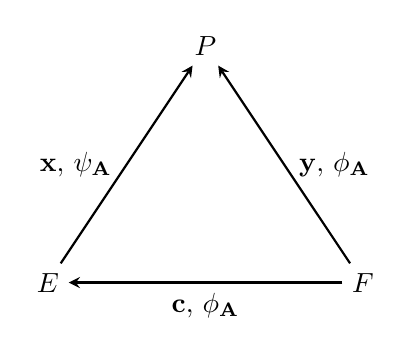
\begin{tikzpicture}[>=stealth, node distance=4cm]
    % Definizione dei nodi
    \node (E) at (0,0) {$E$};
    \node (F) at (4,0) {$F$};
    \node (P) at (2,3) {$P$};

    % Freccia da E a P con etichetta \mathbf{x},\psi_\mathbf{A}
    \draw[->, thick] (E) --  
        node[midway, left] {\(\mathbf{x},\,\psi_{\mathbf{A}}\,\)} (P);

    % Freccia da F a P con etichetta \mathbf{y},\phi_\mathbf{A}
    \draw[->, thick] (F) -- 
        node[midway, right] {\(\,\mathbf{y},\,\phi_{\mathbf{A}}\)} (P);

    % Freccia da F a E con etichetta \mathbf{c},\phi_\mathbf{A}
    \draw[->, thick] (F) -- 
        node[midway, below] {\(\mathbf{c},\,\phi_{\mathbf{A}}\)} (E);
\end{tikzpicture}
\end{center}

\vspace{10pt}

La \ref{dodicii} è la formula del \textbf{cambiamento di coordinate affini dal riferimento} $E \mathbf{e}_1, \dots, \mathbf{e}_n$ \textbf{al riferimento} $F \mathbf{f}_1, \dots, \mathbf{f}_n$.

La \ref{dodicii} dipende solo dalle basi $\psi$ ed $\phi$ e dai punti $E$ ed $F$, le origini nei due riferimenti affini assegnati.

Nel caso in cui lo spazio $\mathbf{A}$ è uno spazio affine reale, due riferimenti affini $E \mathbf{e}_1, \dots, \mathbf{e}_n$ e $F \mathbf{f}_1, \dots, \mathbf{f}_n$ si diranno \textbf{orientati concordemente} 
(\textbf{orientati discordemente}) se le basi $\phi$ ed $\psi$ sono orientate concordemente (orientate discordemente).

\vspace{10pt}

Consideriamo l'insieme $\mathcal{R}$ di tutti i riferimenti affini di $\mathbf{A}$, e in $\mathcal{R}$ diciamo equivalenti due riferimenti se sono orientati concordemente. 
Procedendo in modo simile al caso vettoriale, possiamo verificare che quella che abbiamo definito è effettivamente una relazione di equivalenza, 
e che le classi di equivalenza sono due. Esse si dicono le \textbf{orientazioni di $\mathbf{A}$}. 
L'orientazione cui un dato riferimento $E \mathbf{e}_1, \dots, \mathbf{e}_n \in \mathcal{R}$ appartiene è \textbf{l'orientazione di $\mathbf{A}$ definita da} $E \mathbf{e}_1, \dots, \mathbf{e}_n$.

\vspace{10pt}

Se $\psi_{\mathbf{A}}'=E\mathbf{e}_1, \dots, \mathbf{e}_n$ è un riferimento affine dello spazio affine $\mathbf{A}$ e se un secondo riferimento affine 
assegnato è $\psi_{\mathbf{A}}''=F\mathbf{e}_1, \dots, \mathbf{e}_n$, cioè è ottenuto solo cambiando la posizione dell'origine e lasciando invariata la base dei vettori, 
la formula \ref{dodicii} si riduce alla seguente:
\begin{equation}\label{dodiciquattro}
\mathbf{y} = \mathbf{x} + \mathbf{c}.    
\end{equation}

\vspace{10pt}

\begin{center}
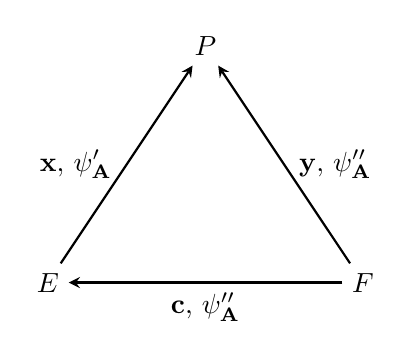
\begin{tikzpicture}[>=stealth, node distance=4cm]
    % Definizione dei nodi
    \node (E) at (0,0) {$E$};
    \node (F) at (4,0) {$F$};
    \node (P) at (2,3) {$P$};

    % Freccia da E a P con etichetta \mathbf{x},\psi_\mathbf{A}
    \draw[->, thick] (E) --  
        node[midway, left] {\(\mathbf{x},\,\psi_{\mathbf{A}}'\,\)} (P);

    % Freccia da F a P con etichetta \mathbf{y},\phi_\mathbf{A}
    \draw[->, thick] (F) -- 
        node[midway, right] {\(\,\mathbf{y},\,\psi_{\mathbf{A}}''\)} (P);

    % Freccia da F a E con etichetta \mathbf{c},\phi_\mathbf{A}
    \draw[->, thick] (F) -- 
        node[midway, below] {\(\mathbf{c},\,\psi_{\mathbf{A}}''\)} (E);
\end{tikzpicture}
\end{center}

\vspace{10pt}

Se invece il secondo riferimento è $E\mathbf{f}_1, \dots, \mathbf{f}_n$, cioè è ottenuto cambiando la base dei vettori, ma non l'origine, la formula \ref{dodicii} diventa
\begin{equation}\label{dodicicinque}
\mathbf{y} = A\mathbf{x}
\end{equation}

\vspace{10pt}

\begin{center}
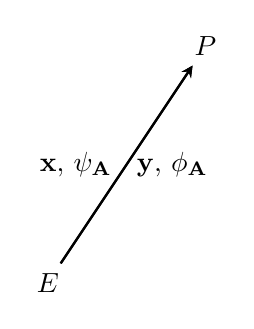
\begin{tikzpicture}[>=stealth, node distance=4cm]
    % Definizione dei nodi
    \node (E) at (0,0) {$E$};
    \node (P) at (2,3) {$P$};

    % Freccia da E a P con etichetta \mathbf{x},\psi_\mathbf{A}
    \draw[->, thick] (E) --  
        node[midway, left] {\(\mathbf{x},\,\psi_{\mathbf{A}}\,\)} (P);
    \draw[->, thick] (E) --  
        node[midway, right] {\(\mathbf{y},\,\phi_{\mathbf{A}}\,\)} (P);
\end{tikzpicture}
\end{center}

\vspace{10pt}

\begin{bxthm}
\begin{prop}
Ogni cambiamento di riferimento affine si può ottenere come la composizione di uno del tipo \ref{dodiciquattro} seguito da uno del tipo \ref{dodicicinque}, o viceversa.     
\end{prop}
\end{bxthm}
\begin{proof}
    Da fare.
\end{proof}

\vspace{10pt}

Siano 
\[ \psi_\mathbf{A}=E\mathbf{e}_1, \dots, \mathbf{e}_n,\quad \phi_\mathbf{A}=F\mathbf{f}_1, \dots, \mathbf{f}_n,\quad \varphi_\mathbf{A}=G\mathbf{g}_1, \dots, \mathbf{g}_n \]
tre riferimenti affini in $\mathbf{A}$, e siano 
\[ \mathbf{x} = (x_1, \dots, x_n),\quad \mathbf{y} = (y_1, \dots, y_n),\quad \mathbf{z} = (z_1, \dots, z_n) \]
i vettori delle coordinate di un punto $P \in \mathbf{A}$ rispetto ad ognuno dei riferimenti dati. 

\vspace{10pt}

\begin{center}
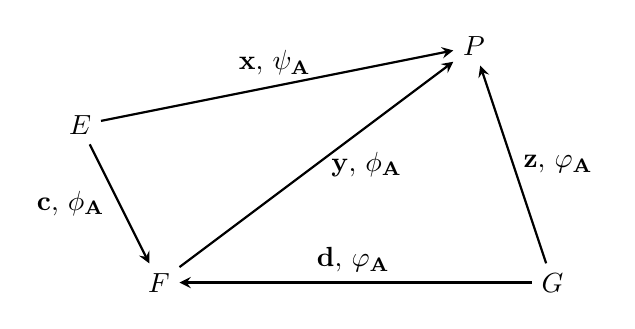
\begin{tikzpicture}[>=stealth, node distance=4cm]
    % Definizione dei nodi
    \node (E) at (1,3) {$E$};
    \node (F) at (2,1) {$F$};
    \node (G) at (7,1) {$G$};
    \node (P) at (6,4) {$P$};

    \draw[->, thick] (E) --  node[midway, above] {\(\mathbf{x},\,\psi_{\mathbf{A}}\,\)} (P);
    \draw[->, thick] (E) --  node[midway, left] {\(\mathbf{c},\,\phi_{\mathbf{A}}\,\)} (F);
    \draw[->, thick] (F) --  node[midway, right] {\(\,\mathbf{y},\,\phi_{\mathbf{A}}\,\)} (P);
    \draw[->, thick] (G) --  node[midway, above] {\(\mathbf{d},\,\varphi_{\mathbf{A}}\,\)} (F);
    \draw[->, thick] (G) --  node[midway, right] {\(\mathbf{z},\,\varphi_{\mathbf{A}}\,\)} (P);
    % Freccia da E a P con etichetta \mathbf{x},\psi_\mathbf{A}
    %\draw[->, thick] (E) --  
    %    node[midway, left] {\(\mathbf{x},\,\psi_{\mathbf{A}}\,\)} (P);

\end{tikzpicture}
\end{center}

\vspace{10pt}

Siano $A=M_{\phi,\psi}(\mathbf{1_V}), B=M_{\varphi,\phi}(\mathbf{1_V})$, e
\[\overrightarrow{EP}=\sum_{j=1}^{n}x_j\mathbf{e}_j,\quad\overrightarrow{FP}=\sum_{j=1}^{n}y_j\mathbf{f}_j,\quad\overrightarrow{GP}=\sum_{j=1}^{n}z_j\mathbf{g}_j\]
Supponiamo che il passaggio dalle coordinate $\mathbf{x}$ alle $\mathbf{y}$ sia dato da 
\[\mathbf{y}=A\mathbf{x}+\mathbf{c}\]
e che quello dalle $\mathbf{y}$ alle $\mathbf{z}$ sia dato da
\[\mathbf{z}=B\mathbf{y}+\mathbf{d}.\]
Allora la formula che esprime il passaggio dalla $\mathbf{x}$ alle $\mathbf{z}$ si ottiene al seguente modo mediante sostituzione:
\[\mathbf{z}=B\mathbf{y}+\mathbf{d} = \mathbf{z}=B(A\mathbf{x}+\mathbf{c})+\mathbf{d}= \mathbf{z}=BA\mathbf{x}+(B\mathbf{c}+\mathbf{d}).\]

\vspace{10pt}

Con le notazioni della \ref{dodicii} la formula che esprime il passaggio dalle coordinate $\mathbf{y}$ alle $\mathbf{x}$, cioè il passaggio inverso di quello dato dalla \ref{dodicii}, è
\begin{equation}\label{dodicisette}
\mathbf{x} = A^{-1} \mathbf{y} - A^{-1} \mathbf{c}.
\end{equation}
Infatti, sostituendo la \ref{dodicii} nel secondo membro della \ref{dodicisette} si ottiene l'identità $\mathbf{x} = \mathbf{x}$.

\vspace{10pt}

\paragraph{Cambiamento di coordinate affini}
Sia $\mathbf{A}$ un $\mathbb{R}$-spazio affine di dimensione $3$, e sia $\mathbf{V}$ lo spazio vettoriale associato. 
Siano 
\[\psi_\mathbf{A}=E\mathbf{e}_1\mathbf{e}_2\mathbf{e}_3,\quad\textup{e}\quad\phi_\mathbf{A}=F\mathbf{f}_1\mathbf{f}_2\mathbf{f}_3\]
due riferimenti affini in $\mathbf{A}$. 
Supponiamo che
\[
\mathbf{f}_1 = \mathbf{e}_1 + \mathbf{e}_2,\quad \mathbf{f}_2 = -\mathbf{e}_1 + \mathbf{e}_3,\quad \mathbf{f}_3 = \mathbf{e}_1 + \mathbf{e}_2 + \mathbf{e}_3,
\]
e che $F$ abbia coordinate $(5,\ -\frac{3}{2},\ \frac{1}{2})$ nel riferimento $\psi_\mathbf{A}$. 
Per conoscere la formula di cambiamento di coordinate dal riferimento $\psi_\mathbf{A}$ al riferimento 
$\phi_\mathbf{A}$ occorre conoscere la matrice $M_{\phi,\psi}(\mathbf{1_V})$, nonché le coordinate $c_1,\ c_2,\ c_3$ di $E$ 
rispetto a $\phi_\mathbf{A}$. Si ha
\[
M_{\psi,\phi}(\mathbf{1_V}) = 
\begin{pmatrix}
1 & -1 & 1 \\
1 & 0 & 1 \\
0 & 1 & 1
\end{pmatrix}
\]
e quindi
\[
M_{\phi,\psi}(\mathbf{1_V}) = M_{\psi,\phi}(\mathbf{1_V})^{-1} =
\begin{pmatrix}
-1 & 2 & -1 \\
-1 & 1 & 0 \\
1 & -1 & 1
\end{pmatrix}\;.
\]
Per determinare $(c_1,\ c_2,\ c_3)$ utilizziamo la matrice $M_{\phi,\psi}(\mathbf{1_V})$ che abbiamo appena calcolato. 
Si ha
\[
c_1\mathbf{f}_1 + c_2\mathbf{f}_2 + c_3\mathbf{f}_3 = \overrightarrow{FE} = -\overrightarrow{EF} = -\left(5\mathbf{e}_1 - \frac{3}{2}\mathbf{e}_2 + \frac{1}{2}\mathbf{e}_3\right).
\]
Pertanto
\[
\begin{pmatrix}
c_1 \\
c_2 \\
c_3
\end{pmatrix}
= M_{\phi,\psi}(\mathbf{1_V})
\begin{pmatrix}
-5 \\
\frac{3}{2} \\
-\frac{1}{2}
\end{pmatrix}
=
\begin{pmatrix}
-1 & 2 & -1 \\
-1 & 1 & 0 \\
1 & -1 & 1
\end{pmatrix}
\begin{pmatrix}
-5 \\
\frac{3}{2} \\
-\frac{1}{2}
\end{pmatrix}
=
\begin{pmatrix}
\frac{17}{2} \\
\frac{13}{2} \\
-7
\end{pmatrix}\;.
\]
In conclusione, la formula del cambiamento di coordinate dal riferimento
$\psi_\mathbf{A}$ al riferimento $\phi_\mathbf{A}$ è
\[
\begin{pmatrix}
y_1 \\
y_2 \\
y_3
\end{pmatrix}
=
\begin{pmatrix}
-1 & 2 & -1 \\
-1 & 1 & 0 \\
1 & -1 & 1
\end{pmatrix}
\begin{pmatrix}
x_1 \\
x_2 \\
x_3
\end{pmatrix}
+
\begin{pmatrix}
\frac{17}{2} \\
\frac{13}{2} \\
-7
\end{pmatrix}
\]
ovvero:
\[
y_1 = -x_1 + 2x_2 - x_3 + \frac{17}{2} \quad\quad
y_2 = -x_1 + x_2 + \frac{13}{2} \quad\quad
y_3 = x_1 - x_2 + x_3 - 7\;.
\]

\vspace{10pt}

\begin{bxthm}
\begin{prop}
Siano \( \psi = \{\mathbf{e}_1, \dots, \mathbf{e}_n\}, \quad \phi = \{\mathbf{f}_1, \dots, \mathbf{f}_n\} \) 
due basi del \( \mathbb{K} \)-spazio vettoriale \( \mathbf{V} \), e siano
\[
\eta = \{\eta_1, \dots, \eta_n\}, \quad \beta = \{\beta_1, \dots, \beta_n\}
\]
le basi di \( \mathbf{V^*} \) duali di \( \psi \) e di \( \phi \) rispettivamente. Allora
\[
M_{\beta, \eta}(\mathbf{1_{V^*}}) = \left[ M_{\psi, \phi}(\mathbf{1_V}) \right]^t.
\]
\end{prop}
\end{bxthm}
\begin{proof}
    Da fare.
\end{proof}

\vspace{50pt}
\subsection{Operatori Lineari}
\vspace{20pt}

\paragraph{Matrice di un endomorfismo rispetto a una base}
\begin{bxthm}
\begin{defn}
Siano \( \mathbf{V} \) un \( \mathbb{K} \)-spazio vettoriale di dimensione finita, e \( \psi = \{\mathbf{e}_1, \ldots, \mathbf{e}_n\} \) una base di \( \mathbf{V} \). 
Per ogni operatore \( F \in \mathrm{end}(\mathbf{V}) \), scriveremo \( M_\psi(F) \) invece di \( M_{\psi,\psi}(F) \), e chiameremo 
\( M_\psi(F) \) la \textbf{matrice di \( F \) rispetto alla base \( \psi \)}.    
\end{defn}
\end{bxthm}

\vspace{10pt}

Dal teorema \ref{dodicidue} segue che l'applicazione
\[M_\psi \colon \mathrm{end}(\mathbf{V}) \to M_n(\mathbb{K}),\quad F \mapsto M_\psi(F)\]
è un isomorfismo di \( \mathbb{K} \)-spazi vettoriali. Si ha $M_\psi(\mathbf{1_V}) = \mathbf{I}_n$ e 
\[ M_\psi(F) \in \mathrm{GL}_n(\mathbb{K})\iff F \in \mathrm{GL}(\mathbf{V}),\]
cioè un operatore \( F \) è un automorfismo se e solo se \( M_\psi(F) \) è invertibile. 
Quindi l'applicazione \( M_\psi \) induce una biezione che denotiamo con lo stesso simbolo:
\[
M_\psi \,:\; \mathrm{GL}(\mathbf{V}) \to \mathrm{GL}_n(\mathbb{K}).
\]
Sia \( \phi = \{\mathbf{f}_1, \ldots, \mathbf{f}_n\} \) un'altra base di \( \mathbf{V} \). 
Dalla proposizione \ref{dodicitre} deduciamo che
\[
M_\phi(F) = M_{\phi,\psi}(\mathbf{1_V}) M_\psi(F) M_{\psi,\phi}(\mathbf{1_V}).
\]
Poiché \( M_{\phi,\psi}(\mathbf{1_V}) = M_{\psi,\phi}(\mathbf{1_V})^{-1} \), otteniamo
\begin{equation}\label{trediciuno}
M_\phi(F) = M_{\psi,\phi}(\mathbf{1_V})^{-1} M_\psi(F) M_{\psi,\phi}(\mathbf{1_V})     
\end{equation}
da cui segue immediatamente che
\[
\det(M_\phi(F)) = \det(M_\psi(F)),
\]
cioè \( \det(M_\psi(F)) \) non dipende dalla base \( \psi \), ma solo da \( F \). 

\vspace{10pt}

\paragraph{Determinante dell'operatore}
\begin{bxthm}
\begin{defn}
Chiameremo pertanto \( \det(M_\psi(F)) \) il \textbf{determinante dell'operatore} \( F \) e lo denoteremo con 
\( \det(F) \), senza dover specificare la matrice \( M_\psi(F) \) attraverso la quale è stato calcolato.    
\end{defn}
\end{bxthm}

\vspace{10pt}

\paragraph{Similitudine tra matrici}
\begin{bxthm}
\begin{defn}
Due matrici \( A, B \in M_n(\mathbb{K}) \) si dicono \textbf{simili} se: 
\[\exists\,M \in \mathrm{GL}_n(\mathbb{K}) \,:\; B = M^{-1} A M.\]
\end{defn}
\end{bxthm}

\vspace{10pt}

\begin{bxthm}
\begin{prop}
La similitudine è una relazione di equivalenza in \( M_n(\mathbb{K}) \).    
\end{prop}
\end{bxthm}
\begin{proof}\hfill
\begin{enumerate}
    \item \textit{Riflessività}:
    \[\forall\,A\in M_n(\mathbb{K}),\quad A = \mathbf{I}_n^{-1} A \mathbf{I}_n;\]
    \item \textit{Simmetria}
    \[\forall\,A,B\in M_n(\mathbb{K}),\quad B = M^{-1} A M\implies A = (MM^{-1}) A (MM^{-1}) = M(M^{-1} A M)M^{-1} = M B M^{-1};\]
    \item \textit{Transitività}
    \[B = M^{-1} A M\; \land\; C = N^{-1} B N\implies C = N^{-1}(M^{-1} A M) N = (MN)^{-1} A (MN).\]
\end{enumerate}
\end{proof}

\vspace{10pt}

\begin{bxthm}
\begin{prop}
Siabo \( \mathbf{V} \) un \( \mathbb{K} \)-spazio vettoriale, \( \dim(\mathbf{V}) = n \), e \( A, B \in M_n(\mathbb{K}) \). 
\( A \) e \( B \) sono simili se e solo se esistono un operatore lineare \( F \in \mathrm{end}(\mathbf{V}) \) e basi \( \psi \) ed \( \phi \) di \( \mathbf{V} \) tali che \( M_\psi(F) = A \) ed \( M_\phi(F) = B \).    
\end{prop}
\end{bxthm}
\begin{proof}
Se \( F, \psi,\phi \) esistono, allora dalla \ref{trediciuno} segue che \( A \) e \( B \) sono simili. 
Supponiamo viceversa che
\begin{equation}\label{tredicidue}
B = M^{-1} A M.    
\end{equation}
Sia \( \psi \) una base arbitraria di \( \mathbf{V} \) e sia \( F = F_A \) l'operatore associato alla matrice \( A \) 
rispetto alla base \( \psi \). Per ogni \( j \in \{1, \ldots, n\} \) sia \( \mathbf{f}_j \) il vettore le cui coordinate rispetto a 
\( \psi \) sono gli elementi della \( j \)-esima colonna di \( M \), cioè 
\[\mathbf{f}_j = \sum_{i=1}^{n}m_{ij}\mathbf{e}_i.\]
Poiché \( M \) ha rango \( n \), i vettori \( \mathbf{f}_1, \ldots, \mathbf{f}_n \) sono linearmente indipendenti 
e quindi \( \{\mathbf{f}_1, \ldots, \mathbf{f}_n\} \) è una base di \( \mathbf{V} \). 
Si ha inoltre
\[
M = M_{\psi,\phi}(\mathbf{1_V}).
\]
Dalla \ref{tredicidue} discende che \( B = M_\phi(F) \).    
\end{proof}

\vspace{10pt}

\paragraph{Operatore diagonalizzabile e base diagonalizzante}
\begin{bxthm}
\begin{defn}
Sia \( \mathbf{V} \) un \( \mathbb{K} \)-spazio vettoriale, \( \dim(\mathbf{V}) = n \). 
Un operatore \( F \in \mathrm{end}(\mathbf{V}) \) si dice \textbf{diagonalizzabile} se esiste una base \( \psi \) 
di \( \mathbf{V} \) tale che \( M_\psi(F) \) sia una matrice diagonale, cioè della forma
\[
\begin{pmatrix}
\lambda_1 & 0 & \cdots & 0 \\
0 & \lambda_2 & \cdots & 0 \\
\vdots & \vdots & \ddots & \vdots \\
0 & 0 & \cdots & \lambda_n
\end{pmatrix}
\]
per opportuni \( \lambda_1, \lambda_2, \ldots, \lambda_n \in \mathbb{K} \). 
Se ciò avviene \( \psi \) è una \textbf{base diagonalizzante} per \( F \).    
\end{defn}
\end{bxthm}

\vspace{10pt}

\paragraph{Matrice diagonalizzabile}
\begin{bxthm}
\begin{defn}
Una matrice \( A \in M_n(\mathbb{K}) \) si dice \textbf{diagonalizzabile} se è simile a una matrice diagonale.
\end{defn}
\end{bxthm}

\vspace{10pt}

Ovviamente, se \( F \in \mathrm{end}(\mathbf{V}) \) e \( \psi \) è una base di \( \mathbf{V} \), 
\( F \) è diagonalizzabile se e solo se \( M_\psi(F) \) è una matrice diagonalizzabile. 
In particolare \( A \in M_n(\mathbb{K}) \) è diagonalizzabile se e solo se l'operatore 
\( F_A \in\mathrm{end}(\mathbb{K}^n) \) definito da \( A \) è diagonalizzabile.
Se \( F \in \mathrm{end}(\mathbf{V}) \) è diagonalizzabile e 
\( \psi \) è una base diagonalizzante per \( F \), si ha
\begin{equation}\label{tredicitre}
F(\mathbf{e}_i) = \lambda_i \mathbf{e}_i, \quad i \in \{1, \ldots, n\}.
\end{equation}
Viceversa, se una base \( \psi \) soddisfacente la \ref{tredicitre} esiste, allora la matrice \( M_\psi(F) \) è diagonale, 
e quindi \( F \) è diagonalizzabile e \( \psi \) è una base diagonalizzante. Si noti che, se \( \dim(\mathbf{V}) = 1 \), allora ogni \( F \in \mathrm{end}(\mathbf{V}) \) è diagonalizzabile e ogni 
base di \( \mathbf{V} \) è diagonalizzante per \( F \). Se \( \dim(\mathbf{V}) \geq 2 \) non tutti gli operatori \( F \in \mathrm{end}(\mathbf{V}) \) 
sono diagonalizzabili. Similmente non tutte le matrici \( A \in M_n(\mathbb{K}) \) sono diagonalizzabili se \( n \geq 2 \).

\vspace{10pt}

In relazione al problema di stabilire l'esistenza di basi diagonalizzanti si presentano in modo naturale le nozioni di \textbf{autovettore} e di \textbf{autovalore}.

\vspace{10pt}

\paragraph{Autovettore, autovalore, e spettro di un operatore}
\begin{bxthm}
\begin{defn}
Siano $\mathbf{V}$ un $\mathbb{K}$-spazio vettoriale, e $F \in \mathrm{end}(\mathbf{V})$. 
Un vettore $\mathbf{v} \in \mathbf{V}$ si dice \textbf{autovettore} di $F$ se 
\[\mathbf{v} \neq \mathbf{0}\;\land\;\exists\,\lambda \in \mathbb{K}\,:\;F(\mathbf{v}) = \lambda \mathbf{v}.\]
$\lambda$ è l'\textbf{autovalore} di $F$ relativo all'autovettore $\mathbf{v}$.
Il sottoinsieme di $\mathbb{K}$ costituito dagli autovalori di $F$ è lo \textbf{spettro} di $F$.
\end{defn}
\end{bxthm}

\vspace{10pt}

Se $A \in M_n(\mathbb{K})$, un autovettore di $A$ è un autovettore $\mathbf{x} \in \mathbb{K}^n$ dell'operatore $F_A \in\mathrm{end}(\mathbb{K}^n)$ definito da $A$, e un autovalore di $A$ è un autovalore di $F_A$.

\vspace{10pt}

\begin{exmp}
Se $F = \mathbf{1_V}$, ogni $\mathbf{v} \neq \mathbf{0}$ è un autovettore di $F$ con autovalore $\lambda = 1$.     
\end{exmp}

\vspace{10pt}

\begin{exmp}
Se $F$ è un operatore tale che $\ker(F) \neq \langle\mathbf{0}\rangle$, ogni $\mathbf{v} \in \ker(F) \setminus \langle\mathbf{0}\rangle$ è un autovettore di $F$ con autovalore $\lambda = 0$.    
\end{exmp}

\vspace{10pt}

Diamo qui di seguito alcune semplici proprietà degli autovettori e degli autovalori di un operatore $F \in \mathrm{end}(\mathbf{V})$. 
Supponiamo $\dim(\mathbf{V}) = n \geq 1$.

\vspace{10pt}

\begin{bxthm}
\begin{prop}
    L'autovalore relativo a un autovettore $\mathbf{v}$ è univocamente determinato.
\end{prop}
\end{bxthm}
\begin{proof}
    Se $\lambda \mathbf{v} = F(\mathbf{v}) = \mu \mathbf{v}$ per qualche $\lambda, \mu \in \mathbb{K}$, allora $(\lambda - \mu)\mathbf{v} = \mathbf{0}$, poiché $\mathbf{v} \neq \mathbf{0}$, dev'essere $\lambda - \mu = 0$, cioè $\lambda = \mu$.    
\end{proof}

\vspace{10pt}

\begin{bxthm}
\begin{prop}\label{trediciseii}
Se $\mathbf{v}_1, \mathbf{v}_2 \in \mathbf{V}$ sono autovettori relativi allo stesso autovalore $\lambda$, allora per ogni $c_1, c_2 \in \mathbb{K}$ il vettore 
$c_1 \mathbf{v}_1 + c_2 \mathbf{v}_2$, se non è il vettore nullo, è ancora un autovettore con autovalore $\lambda$.    
\end{prop}
\end{bxthm}
\begin{proof}
Si ha
\[
F(c_1 \mathbf{v}_1 + c_2 \mathbf{v}_2) = c_1 F(\mathbf{v}_1) + c_2 F(\mathbf{v}_2) = c_1 \lambda \mathbf{v}_1 + c_2 \lambda \mathbf{v}_2 = \lambda (c_1 \mathbf{v}_1 + c_2 \mathbf{v}_2).
\]    
\end{proof}

\vspace{10pt}

\paragraph{Autospazio relativo a un'autovalore}
\begin{bxthm}
\begin{defn}
Dalla \ref{trediciseii} segue che l'insieme
\[
\mathbf{V}_\lambda(F) = \{\mathbf{v} \in \mathbf{V} \,:\; \mathbf{v} \text{ è un autovettore di } F \text{ con autovalore } \lambda \} \cup \{\mathbf{0}\}
\]
è un sottospazio vettoriale di $\mathbf{V}$, detto \textbf{l'autospazio relativo all'autovalore} $\lambda$. 
Per una matrice $A \in M_n(\mathbb{K})$ si definisce \textbf{l'autospazio} $\mathbf{V}_\lambda(A)$ \textbf{relativo all'autovalore} $\lambda$ come il sottospazio di $\mathbb{K}^n$ 
\[\mathbf{V}_\lambda(A) = \mathbf{V}_\lambda(F_A).\]
\end{defn}
\end{bxthm}

\vspace{10pt}

\begin{bxthm}
\begin{prop}\label{quelloserio}
Se $\mathbf{v}_1, \dots, \mathbf{v}_k \in \mathbf{V}$ sono autovettori relativi agli autovalori $\lambda_1, \dots, \lambda_k$ e se questi $\lambda_i$ con $i\in\{1,\ldots,k\}$
sono a due a due distinti, allora $\mathbf{v}_1, \dots, \mathbf{v}_k$ sono linearmente indipendenti.
\end{prop}
\end{bxthm}
\begin{proof}
L'asserzione è banalmente vera se $k = 1$, perché $\mathbf{v}_1 \neq 0$. 
Procediamo per induzione su $k$, e supponiamo $k \geq 2$. Se
\begin{equation}\label{trediciquattro}
\sum_{i=1}^{k}c_i\mathbf{v}_i=0, 
\end{equation}
allora, applicando $F$ a entrambi i membri, si ha anche
\[
\sum_{i=1}^{k}c_iF(\mathbf{v}_i)=0,
\]
cioè
\begin{equation}\label{tredicicinque}
\sum_{i=1}^{k}c_i\lambda_i\mathbf{v}_i=0.
\end{equation}
D'altra parte, moltiplicando ambo i membri della \ref{trediciquattro} per $\lambda_1$, si ottiene
\begin{equation}\label{tredicisei}
    \lambda_1\left(\sum_{i=1}^{k}c_i\mathbf{v}_i\right)=\sum_{i=1}^{k}\lambda_1c_i\mathbf{v}_i=0
\end{equation}
e sottraendo la \ref{tredicisei} dalla \ref{tredicicinque}:
\begin{equation}\label{tredicisette}
    \sum_{i=1}^{k}c_i\lambda_i\mathbf{v}_i-\sum_{i=1}^{k}\lambda_1c_i\mathbf{v}_i=\sum_{i=1}^{k}\left(c_i\lambda_i\mathbf{v}_i-\lambda_1c_i\mathbf{v}_i\right)=\sum_{i=1}^{k}c_i\left(\lambda_i\mathbf{v}_i-\lambda_1\mathbf{v}_i\right)=\sum_{i=1}^{k}c_i\left(\lambda_i-\lambda_1\right)\mathbf{v}_i=0.
\end{equation}
Per l'ipotesi induttiva $\mathbf{v}_2, \ldots, \mathbf{v}_k$ sono linearmente indipendenti, e quindi i coefficienti del primo membro della 
\ref{tredicisette} sono tutti uguali a $0$. Poiché $\lambda_j - \lambda_1 \neq 0$ per ogni $j\in\{2,\ldots,k\}$, si deduce che 
$c_2 = \cdots = c_k = 0$. Quindi la \ref{trediciquattro} si riduce a $c_1 \mathbf{v}_1 = 0$, e quest'identità implica 
che anche $c_1 = 0$, perché $\mathbf{v}_1 \neq 0$.    
\end{proof}

\vspace{10pt}

\begin{bxthm}
\begin{prop}
Se ogni $\mathbf{v} \in \mathbf{V} \setminus \{\mathbf{0}\}$ è un autovettore di $F$, allora 
\[\exists\,\lambda \in \mathbb{K}\,:\;F = \lambda \, \mathbf{1_V}.\]
\end{prop}
\end{bxthm}
\begin{proof}
Se $\dim(\mathbf{V}) = 1$ l'asserzione è ovvia. Possiamo quindi supporre $\dim(\mathbf{V}) \geq 2$. 
Sia $\{\mathbf{e}_1, \ldots, \mathbf{e}_n\}$ una base di $\mathbf{V}$. Dall'ipotesi segue che esistono 
$\lambda_1, \lambda_2, \ldots, \lambda_n \in \mathbb{K}$ tali che $F(\mathbf{e}_i) = \lambda_i \mathbf{e}_i$, 
per $i \in \{1, \ldots, n\}$. Siano $1 \leq i,\, j \leq n$ due indici distinti, e sia $\mathbf{v}_{ij} = \mathbf{e}_i + \mathbf{e}_j$. 
Per l'ipotesi esiste $\lambda_{ij} \in \mathbb{K}$ tale che
\[
F(\mathbf{v}_{ij}) = \lambda_{ij} \mathbf{v}_{ij} = \lambda_{ij} \mathbf{e}_i + \lambda_{ij} \mathbf{e}_j.
\]
D'altra parte si ha
\[
F(\mathbf{v}_{ij}) = F(\mathbf{e}_i + \mathbf{e}_j) = F(\mathbf{e}_i) + F(\mathbf{e}_j) = \lambda_i \mathbf{e}_i + \lambda_j \mathbf{e}_j,
\]
e, per l'indipendenza lineare di $\mathbf{e}_i$ ed $\mathbf{e}_j$, deduciamo che $\lambda_i = \lambda_j = \lambda_{ij}$. 
In conclusione $\lambda_1 = \lambda_2 = \cdots = \lambda_n$, e l'asserto è provato.    
\end{proof}

\vspace{10pt}

In pratica nella ricerca degli autovalori di un operatore o di una matrice si utilizza il cosiddetto \textbf{polinomio caratteristico}. 
La sua definizione si avvale del seguente semplice risultato.

\vspace{10pt}

\begin{bxthm}
\begin{prop}\label{tredicinovee}
Sia $\mathbf{V}$ uno spazio vettoriale di dimensione finita e sia $F \in \mathrm{end}(\mathbf{V})$. 
Uno scalare $\lambda \in \mathbb{K}$ è un autovalore di $F$ se e solo se l'operatore
\[
F - \lambda\mathbf{1_V} : \mathbf{V} \to \mathbf{V},\quad\mathbf{v}\to F(\mathbf{v}) - \lambda \mathbf{v},
\]
non è un isomorfismo, o, equivalentemente, se e solo se 
\[\det(F - \lambda \, \mathbf{1_V}) = 0.\]
\end{prop}
\end{bxthm}
\begin{proof}
$F - \lambda \mathbf{1_V}$ non è un isomorfismo se e solo se $\mathrm{N}(F - \lambda\mathbf{1_V}) \neq \langle\mathbf{0}\rangle$, 
cioè se 
\[\exists\,\mathbf{v}\in\mathbf{V}\setminus\{\mathbf{0}\}\,:\;(F - \lambda \mathbf{1_V})(\mathbf{v}) = \mathbf{0},\]
ovvero tale che
\begin{equation}\label{trediciotto}
F(\mathbf{v}) = \lambda \mathbf{v}.
\end{equation}
La \ref{trediciotto} afferma che $F$ possiede l'autovettore $\mathbf{v}$ con autovalore $\lambda$.
Sia $\psi = \{\mathbf{e}_1, \dots, \mathbf{e}_n\}$ una base di $\mathbf{V}$. 
La matrice associata all'operatore $\lambda \mathbf{1_V}$ è
\[
\begin{pmatrix}
\lambda & 0 & \cdots & 0 \\
0 & \lambda & \cdots & 0 \\
\vdots & \vdots & \ddots & \vdots \\
0 & 0 & \cdots & \lambda \\
\end{pmatrix}
\]
e, se $A = (a_{ij}) = M_{\psi}(F)$, allora
\[
M_{\psi}(F - \lambda \mathbf{1_V}) = 
\begin{pmatrix}
a_{11} - \lambda & a_{12} & \cdots & a_{1n} \\
a_{21} & a_{22} - \lambda & \cdots & a_{2n} \\
\vdots & \vdots & \ddots & \vdots \\
a_{n1} & a_{n2} & \cdots & a_{nn} - \lambda \\
\end{pmatrix}
\]    
\end{proof}

\vspace{10pt}

\paragraph{Polinomio caratteristico}
\begin{bxthm}
\begin{defn}
Sia $A \in M_n(\mathbb{K})$ e sia $T$ un'indeterminata. Il determinante
\[
P_A(T) = \lvert A - T \mathbf{I}_n \rvert =
\begin{vmatrix}
\,a_{11} - T & a_{12} & \cdots & a_{1n} \\
a_{21} & a_{22} - T & \cdots & a_{2n} \\
\vdots & \vdots & \ddots & \vdots \\
a_{n1} & a_{n2} & \cdots & a_{nn} - T \,\\
\end{vmatrix}
\]
è un polinomio di grado $n$ in $T$, detto \textbf{polinomio caratteristico} di $A$.    
Se $F\in\mathrm{end}(\mathbf{V})$, $\psi=\{\mathbf{e}_1,\ldots,\mathbf{e}_n\}$ è una base di $\mathbf{V}$ 
e $A=M_\psi(F)$, allora $P_A(T)$ è il \textbf{polinomio caratteristico} di $F$, e si denota con $P_F(T)$
\end{defn}
\end{bxthm}

\vspace{10pt}

La definizione di $P_F(T)$ è indipendente dalla base $\psi$, come vediamo dalla seguente proposizione:

\vspace{10pt}

\begin{bxthm}
\begin{prop}
    Due matrici simili, come sono quelle che rappresentano $F$ in due basi diverse, hanno lo stesso polinomio caratteristico.
\end{prop}
\end{bxthm}
\begin{proof}
Siano $A$ e $B$ due matrici simili, cioè si abbia $B = M^{-1}AM$, per qualche $M \in \mathrm{GL}_n(\mathbb{K})$. 
Allora
\[B-T\mathbf{I}_n=M^{-1}AM-T(M^{-1}M)=M^{-1}(AM-TM)=M^{-1}(A-T\mathbf{I}_n)M.\]
Pertanto 
\[|B - T\mathbf{I}_n| = |M^{-1}| \cdot |A - T\mathbf{I}_n| \cdot |M| = |A - T\mathbf{I}_n|.\]
\end{proof}

\vspace{10pt}

\begin{note}
Il coefficiente di $T^n$ in $P_A(T)$ è $(-1)^n$, e quindi $(-1)^n P_A(T)$ è un polinomio monico.    
\end{note}

\vspace{10pt}

Dalla proposizione \ref{tredicinovee} deduciamo il seguente corollario.

\vspace{10pt}

\begin{bxthm}
\begin{cor}\label{trediciundici}
    Sia $\mathbf{V}$ uno spazio vettoriale di dimensione finita $n$, e sia $F \in \mathrm{end}(\mathbf{V})$. 
    Allora $\lambda \in \mathbb{K}$ è un autovalore di $F$ se e solo se $\lambda$ è radice di $P_F(T)$. 
    In particolare $F$ possiede al più $n$ autovalori distinti.    
\end{cor}    
\end{bxthm}
\begin{proof}
La prima asserzione è una riformulazione della proposizione \ref{tredicinovee}. 
Poiché $P_A(T)$ ha grado uguale a $\dim(\mathbf{V})$, l'ulteriore asserzione segue dal fatto che un polinomio di 
grado $n$ a coefficienti in $\mathbb{K}$ possiede al più $n$ radici in $\mathbb{K}$.    
\end{proof}

\vspace{10pt}

Il corollario \ref{trediciundici} fornisce un metodo pratico per calcolare gli autovalori e autovettori di un operatore. 

\vspace{10pt}

Il problema di stabilire se un operatore è diagonalizzabile è un problema di ricerca di autovalori e dei relativi autovettori. 

\vspace{10pt}

\begin{bxthm}
\begin{prop}\label{tredicidodici}
Sia $\mathbf{V}$ uno spazio vettoriale di dimensione finita. Un operatore $F \in \mathrm{end}(\mathbf{V})$ 
è diagonalizzabile se e solo se $\mathbf{V}$ possiede una base costituita da autovettori di $F$.
\end{prop}
\end{bxthm}
\begin{proof}
    Segue immediatamente dalla \ref{tredicitre}.
\end{proof}

\vspace{10pt}

Il risultato seguente dà una condizione necessaria e sufficiente affinché un operatore sia diagonalizzabile.

\vspace{10pt}

\begin{bxthm}
\begin{thm}\label{tredicitredici}
Sia $\mathbf{V}$ un $\mathbb{K}$-spazio vettoriale, $\dim(\mathbf{V}) = n$, e sia $F \in \mathrm{end}(\mathbf{V})$.
Se $\{\lambda_1, \ldots, \lambda_k\} \subset \mathbf{K}$ è lo spettro di $F$, allora si ha:
\begin{equation}\label{tredicinove}
    \sum_{i=1}^{k}\dim(\mathbf{V}_{\lambda_i}(F))\leq n
\end{equation}
e l'uguaglianza sussiste se e solo se $F$ è diagonalizzabile.    
\end{thm}
\end{bxthm}
\begin{proof}
Per ogni $i \in\{1,\ldots,k\}$ poniamo $d(i) = \dim(V_{\lambda_i}(F))$, e sia $\{e_{i1}, \ldots e_{id(i)}\}$ una base di $V_{\lambda_i}(F)$. 
In virtù della proposizione \ref{tredicidodici} sarà sufficiente dimostrare che i vettori
\[\mathbf{e}_{11}, \ldots, \mathbf{e}_{1d(1)},\; \mathbf{e}_{21}, \ldots, \mathbf{e}_{2d(2)},\; \ldots,\; \mathbf{e}_{k1}, \ldots, \mathbf{e}_{kd(k)}\]
sono linearmente indipendenti.
Supponiamo che si abbia
\[ \mathbf{0} = \sum_{j=1}^{d(1)}c_{1j}\mathbf{e}_{1j}+\sum_{j=1}^{d(2)}c_{2j}\mathbf{e}_{2j}+\ldots+\sum_{j=1}^{d(k)}c_{kj}\mathbf{e}_{kj} \]
cioè
\begin{equation}\label{tredicidieci}
    \mathbf{0} = \sum_{i=1}^{k}\sum_{j=1}^{d(i)}c_{ij}\mathbf{e}_{ij}
\end{equation}
per opportuni scalari $c_{ij}$.
Ponendo 
\[\mathbf{v}_i = \sum_{j=1}^{d(i)}c_{ij}\mathbf{e}_{ij},\]
si ha $\mathbf{v}_i \in V_{\lambda_i}(F)$ e la \ref{tredicidieci} può essere riscritta nella forma seguente:
\begin{equation}\label{trediciundiciio}
\mathbf{0} = \sum_{i=1}^{k}\mathbf{v}_i
\end{equation}
Poiché 
\[\mathbf{v}_i = \mathbf{0}\iff c_{i1} = c_{i2} = \ldots = c_{id(i)} = 0,\]
sarà sufficiente dimostrare che 
\[\mathbf{v}_1 = \mathbf{v}_2 = \ldots = \mathbf{v}_k = \mathbf{0}.\]
Se $\mathbf{v}_i \neq \mathbf{0}$, allora $\mathbf{v}_i$ è un autovettore relativo a $\lambda_i$ e dalla \ref{quelloserio} 
segue che $\{\mathbf{v}_1, \mathbf{v}_2, \ldots, \mathbf{v}_k\} \setminus \{\mathbf{0}\}$ è un insieme di vettori linearmente indipendenti. 
Quindi il secondo membro della \ref{trediciundiciio} può essere uguale a $\mathbf{0}$ se e solo se tutti gli addendi sono $\mathbf{0}$.    
\end{proof}

\vspace{10pt}

Un caso particolare importante del teorema \ref{tredicitredici} è il seguente immediato corollario.

\vspace{10pt}

\begin{bxthm}
\begin{cor}\label{trediciquattordici}
    Se $\dim(\mathbf{V}) = n$ ed $F \in \mathrm{end}(\mathbf{V})$ possiede $n$ autovalori distinti, allora $F$ è diagonalizzabile.
\end{cor}
\end{bxthm}

\vspace{10pt}

Si noti che la condizione sufficiente di diagonalizzabilità espressa dal corollario \ref{trediciquattordici} non è necessaria. 
Infatti l'operatore $\mathbf{1_V}$ è diagonalizzabile qualunque sia $n = \dim(\mathbf{V})$, ma possiede l'unico autovalore $\lambda = 1$.

\vspace{10pt}

Il corollario \ref{trediciundici} fornisce un metodo pratico per calcolare autovettori e autovalori di un operatore o di una matrice. 
Scegliendo una base di $\mathbf{V}$ ci si riduce a considerare il solo caso delle matrici. Sia dunque assegnata $A \in M_n(\mathbb{K})$. 
Si cominci con il calcolare gli eventuali autovalori, che si trovano calcolando il polinomio caratteristico $P_A(T)$ e le sue radici 
in $\mathbb{K}$. Per ogni autovalore $\lambda \in \mathbb{K}$, il sistema omogeneo di $n$ equazioni nelle 
$n$ incognite $\mathbf{X} = {}^t(X_1, \ldots, X_n)$:
\[(A - \lambda I_n) \mathbf{X} = \mathbf{0}\]
ha rango $r < n$ e possiede quindi soluzioni non banali. Lo spazio delle soluzioni è l'autospazio $V_\lambda(A)$. 
Se la somma delle dimensioni degli autospazi così trovati al variare di $\lambda$ è tra tutte le radici di $P_A(T)$ uguale a $n$, allora $A$ è diagonalizzabile, 
per il teorema \ref{tredicitredici}. Una base diagonalizzante si ottiene scegliendo una base di ciascun autospazio e prendendo l'unione.
Ciò fornisce in linea di principio un metodo di calcolo di tutti i vettori di una base diagonalizzante e della matrice del corrispondente cambiamento di base. 
Si osservi che un operatore può non avere autovalori, e quindi neanche autovettori, perché il polinomio caratteristico $P_A(T)$ può non avere radici 
in $\mathbb{K}$. Se però $\mathbb{K}=\mathbb{C}$, allora dal teorema fondamentale dell'algebra segue che $P_A(T)$ possiede radici in 
$\mathbb{C}$. Pertanto: \emph{ogni operatore di uno spazio vettoriale complesso di dimensione finita possiede necessariamente almeno un autovalore, e 
quindi possiede autovettori}. Ciò non significa necessariamente che l'operatore sia diagonalizzabile. 
Se $\mathbb{K} = \mathbb{R}$ può accadere che un operatore di uno spazio $\mathbf{V}$ non possieda autovalore, allora il polinomio caratteristico non ha 
grado dispari, e quindi possiede almeno una radice reale. In conclusione, \emph{ogni operatore di uno spazio vettoriale reale di dimensione dispari possiede almeno un autovalore 
e quindi possiede autovettori}.

\vspace{10pt}

Il polinomio caratteristico della matrice identità $\mathbf{I}_n$ è
\[P_{\,\mathbf{I}_n}(T) = (1 - T)^n.\]

\vspace{10pt}

Il polinomio caratteristico della matrice nulla $n \times n$ è
\[P_{\mathit{0}}(T) = (-1)^n T^n.\]

\vspace{10pt}

In entrambi i casi l'unico autospazio della matrice è $\mathbb{K}^n$.

\vspace{10pt}

Se $A = (a_{ij}) \in M_n(\mathbb{K})$ è una matrice triangolare (superiore o inferiore), si ha
\[P_A(T) = (a_{11} - T)(a_{22} - T) \cdots (a_{nn} - T).\]
Se $a_{11}, a_{22}, \ldots, a_{nn}$ sono distinti, allora, per il corollario \ref{trediciquattordici}, $A$ 
è diagonalizzabile perché possiede $n$ autovalori distinti altrimenti in generale non è vero.    

\vspace{10pt}

\begin{exmp}\label{ex:tre}
La matrice $n \times n$, $n \geq 2$,
\[
A = \begin{pmatrix}
0 & 1 & 0 & \cdots & 0 \\
0 & 0 & 1 & \cdots & 0 \\
\vdots & \vdots & \vdots & \ddots & \vdots \\
0 & 0 & 0 & \cdots & 1 \\
0 & 0 & 0 & \cdots & 0
\end{pmatrix} \in M_n(\mathbb{K})
\]
ha polinomio caratteristico
\[
P_A(T) = (-1)^n T^n
\]
e quindi possiede l'unico autovalore $\lambda = 0$. Da ciò segue che se $A$ fosse diagonalizzabile sarebbe simile alla matrice $\mathbf{0}$. Ma $\mathbf{0}$ è simile soltanto a sé stessa. Infatti per ogni $M \in GL_n(\mathbb{K})$ si ha
\[
M^{-1}\mathbf{0}M = \mathbf{0}.
\]
Quindi $A$ non è diagonalizzabile.    
\end{exmp}

\vspace{10pt}

\begin{exmp}
La matrice
\[
B = A + \mathbf{I}_n = \begin{pmatrix}
1 & 1 & 0 & \cdots & 0 & 0 \\
0 & 1 & 1 & \cdots & 0 & 0 \\
\vdots & \vdots & \vdots & \ddots & \vdots & \vdots \\
0 & 0 & 0 & \cdots & 1 & 1 \\
0 & 0 & 0 & \cdots & 0 & 1
\end{pmatrix} \in M_n(\mathbb{K})
\]
ha polinomio caratteristico $P_B(T) = (1 - T)^n$, uguale a quello della matrice $\mathbf{I}_n$. 
$B$ non è diagonalizzabile, perché se lo fosse sarebbe simile a $\mathbf{I}_n$, la quale invece è simile solo a sé 
stessa: infatti $M^{-1}\mathbf{I}_nM = \mathbf{I}_n$ per ogni $M \in \mathrm{GL}_n(\mathbb{K})$.    
\end{exmp}

\vspace{10pt}

\begin{exmp}
La matrice
\[
A = \begin{pmatrix}
0 & 1 \\
-1 & 0
\end{pmatrix} \in M_2(\mathbb{R})
\]
ha polinomio caratteristico $1 + T^2$. Poiché questo polinomio non ha radici reali, $A$ non possiede autovalori né autovettori in $\mathbb{R}^2$. Se però $A$ viene considerata come una matrice ad elementi complessi, allora essa possiede i due autovalori distinti $\lambda = \pm i$.    
Per il corollario \ref{trediciquattordici}, $A$ è diagonalizzabile in $M_2(\mathbb{C})$, ed è simile alla matrice diagonale
\[
B = \begin{pmatrix}
i & 0 \\
0 & -i
\end{pmatrix}.
\]

Per trovare la matrice $M$ tale che $B = M^{-1}AM$, dobbiamo trovare una base di $\mathbb{C}^2$ costituita da autovettori di $A$, il che equivale a trovare un autovettore per ciascuno dei due autovalori. Possiamo procedere nel seguente modo.

Per la proposizione \ref{tredicinovee} gli autovettori relativi a $\lambda = i$ sono gli elementi del nucleo 
di $A - i\mathbf{I}_2$, cioè sono le soluzioni del sistema omogeneo
\[
\begin{matrix}
-iX + Y = 0 \\
-X - iY = 0    
\end{matrix}\;,
\]
che ha rango $1$, ed è quindi equivalente alla prima equazione. 
Soluzioni sono i vettori della forma $(t, it)$, i quali, al variare di $t \in \mathbb{C}$, 
descrivono l'autospazio $\mathbb{C}^2_i(A)$. Prendendo ad esempio $t = 1$ si ottiene l'autovettore $(1, i)$ 
relativo a $\lambda = i$. Analogamente, considerando il sistema omogeneo corrispondente a $A + i\mathbf{I}_2$, 
otteniamo i vettori della forma $(t, -it)$, e quindi $(i,1)$ è un autovettore relativo a $\lambda = -i$. 
La base $\phi = \{(1, i), (i,1)\}$ è diagonalizzante. Detta $\psi$ la base canonica, si ha

\[
M = M_{\psi,\phi}(\mathbf{1}) = \begin{pmatrix}
1 & i \\
i & 1
\end{pmatrix}
\]

e

\[
M^{-1}AM = \begin{pmatrix}
\frac{1}{2} & -\frac{i}{2} \\
-\frac{i}{2} & \frac{1}{2}
\end{pmatrix}
\begin{pmatrix}
0 & 1 \\
-1 & 0
\end{pmatrix}
\begin{pmatrix}
1 & i \\
i & 1
\end{pmatrix}
=
\begin{pmatrix}
i & 0 \\
0 & -i
\end{pmatrix}.
\]
\end{exmp}

\vspace{10pt}

\paragraph{Molteplicità geometrica e algebrica}
\begin{bxthm}
\begin{defn}
Sia $\mathbf{V}$ un $\mathbb{K}$-spazio vettoriale di dimensione finita. Sia $F \in \mathrm{end}(\mathbf{V})$ e sia $\lambda \in \mathbb{K}$ un 
autovalore di $F$. La $\dim(\mathbf{V}_\lambda(F))$ si dice \textbf{molteplicità geometrica} di $\lambda$ per $F$. 
La \textbf{molteplicità algebrica} di $\lambda$ per $F$ è la molteplicità $h(\lambda)$ di $\lambda$ come 
radice del polinomio caratteristico di $F$.    
\end{defn}
\end{bxthm}

\vspace{10pt}

In generale la molteplicità geometrica e quella algebrica sono diverse. 
Ciò accade ad esempio per le matrici $A$ e $B$ dell'esempio \ref{ex:tre}. 
Per $A$ si ha infatti, evidentemente, $h(0) = n$, mentre per $B$ si ha $h(1) = n$. 
D'altra parte $A$ non è diagonalizzabile e quindi $\dim(V_0(A)) < n$. Similmente per $B$.

\vspace{10pt}

\begin{bxthm}
\begin{prop}
Per ogni $F \in \mathrm{end}(\mathbf{V})$ e $\lambda \in \mathbb{K}$ autovalore di $F$ sussiste la disuguaglianza
\begin{equation}\label{tredicidodicii}
\dim(\mathbf{V}_\lambda(F)) \leq h(\lambda),    
\end{equation}
cioè la molteplicità geometrica non supera la molteplicità algebrica.    
\end{prop}    
\end{bxthm}
\begin{proof}
Supponiamo che $d = \dim(\mathbf{V}_\lambda(F)) \geq 1$, e sia $\psi=\{\mathbf{e}_1, \dots, \mathbf{e}_n\}$ una 
base di $\mathbf{V}$ tale che $\{\mathbf{e}_1, \dots, \mathbf{e}_d\}$ sia una base di $\mathbf{V}_\lambda(F)$. 
Si ha
\[
A = M_\psi(F) = \begin{pmatrix}
\lambda \mathbf{I}_d & B \\
\mathbf{0} & C
\end{pmatrix}
\]
dove $B \in M_{d, n-d}(\mathbb{K})$, $\mathbf{0} \in M_{n-d,d}(\mathbb{K})$ è la matrice nulla, e 
$C \in M_{n-d, n-d}(\mathbf{K})$. Sviluppando $|A - T \mathbf{I}_n|$ con la regola di Laplace rispetto 
alle prime $d$ righe si trova
\[
P_F(T) = (\lambda - T)^d p(T),
\]
dove $p(T) = P_C(T)$ è un polinomio di grado $n - d$. Pertanto $h(\lambda) \geq d$.    
\end{proof}

\vspace{10pt}

Se il campo $\mathbb{K}$ è algebricamente chiuso e $\lambda_1, \dots, \lambda_k$ sono gli autovalori di $F$, si ha
\[
h(\lambda_1) + \dots + h(\lambda_k) = n.
\]

\vspace{10pt}

Pertanto, dalla \ref{tredicidodicii} e dal teorema \ref{tredicitredici} segue che:

\vspace{10pt}

\begin{bxthm}
\begin{cor}
Se il campo $\mathbb{K}$ è algebricamente chiuso l'operatore $F$ è diagonalizzabile se e solo se per ogni autovalore $\lambda$ di $F$ si ha
\[
\dim(\mathbf{V}_\lambda(F)) = h(\lambda),
\]
cioè se e solo se la molteplicità geometrica e la molteplicità algebrica di ogni autovalore $\lambda$ coincidono.    
\end{cor}    
\end{bxthm}

\vspace{10pt}

\begin{bxthm}
\begin{prop}
Se $A = (a_{ij}) \in M_2(\mathbb{K})$, allora si ha
\[
P_A(T) = T^2 - \mathrm{tr}(A)\, T + \det(A),
\]
dove $\mathrm{tr}(A) = a_{11} + a_{22}$ è la \textbf{traccia} di $A$.    
\end{prop}
\end{bxthm}
\begin{proof}
    Da fare.
\end{proof}

\vspace{10pt}

\begin{bxthm}
\begin{prop}
Sia
\[
P(T) = g_0 + g_1 T + \dots + g_{n-1} T^{n-1} + T^n
\]
un polinomio monico di grado $n$ a coefficienti in $\mathbb{K}$, e sia
\[
M_P =
\begin{pmatrix}
0 & 0 & \cdots & 0 & -g_0 \\
1 & 0 & \cdots & 0 & -g_1 \\
0 & 1 & \cdots & 0 & -g_2 \\
\vdots & \vdots & \ddots & \vdots & \vdots \\
0 & 0 & \cdots & 1 & -g_{n-1}
\end{pmatrix}
\]
Il polinomio caratteristico di $M_P$ è uguale a $(-1)^n P(T)$.     
\end{prop}
\end{bxthm}
\begin{proof}
Se $n = 1$, l'affermazione è evidente: $M_P - T = -g_0 - T$. 
Procediamo per induzione su $n$, e supponiamo $n \geq 2$. Si ha
\[
|M_P - T \mathbf{I}_n| =
\begin{vmatrix}
-T & 0 & \cdots & 0 & -g_0 \\
1 & -T & \cdots & 0 & -g_1 \\
0 & 1 & \cdots & 0 & -g_2 \\
\vdots & \vdots & \ddots & \vdots & \vdots \\
0 & 0 & \cdots & 1 & -g_{n-1} - T
\end{vmatrix}
=
\]

\[
= -T 
\begin{vmatrix}
- T & \cdots & 0 &  -g_1 \\
1 & \cdots & 0 &  -g_2 \\
\vdots & \vdots &   & \vdots \\
0 & 1 & \cdots &  -g_{n-1}-T
\end{vmatrix}
+ (-1)^n g_0 
\begin{vmatrix}
1 & -T &  \cdots & 0 \\
0 & 1 &  \cdots & 0 \\
\vdots & \vdots &  & \vdots \\
0 & 0 &  \cdots & 1
\end{vmatrix}
\]

\[
= -T(-1)^{n-1}(g_1 + g_2 T + \dots + g_{n-1} T^{n-2} + T^{n-1}) + (-1)^n g_0 = (-1)^n P(T),
\]
dove il valore del primo determinante è dedotto dall'ipotesi induttiva.    
\end{proof}

\vspace{10pt}

Questa proposizione dimostra che per ogni polinomio monico di grado $n \geq 1$ in $\mathbb{K}[T]$ esistono 
matrici quadrate di ordine $n$ di cui esso, o il suo opposto, a seconda che $n$ sia pari o dispari, è il 
polinomio caratteristico.

\vspace{50pt}
\part{Geometria Euclidea}
\vspace{50pt}

\section{Forme bilineari e quadratiche}
\vspace{20pt}

\paragraph{Forme bilineari}
\begin{bxthm}
\begin{defn}
Sia \( \mathbf{V} \) un \( \mathbb{K} \)-spazio vettoriale. Un'applicazione
\[
b \,:\; \mathbf{V}^2 \rightarrow \mathbb{K}
\]
si dice \textbf{forma bilineare su} \( \mathbf{V} \) se è lineare in ognuno dei due argomenti, cioè se soddisfa 
le seguenti condizioni:
\begin{itemize}
    \item[FB1] \( b(\mathbf{v} + \mathbf{v}', \mathbf{w}) = b(\mathbf{v}, \mathbf{w}) + b(\mathbf{v}', \mathbf{w}) \)
    \item[FB2] \( b(\mathbf{v}, \mathbf{w} + \mathbf{w}') = b(\mathbf{v}, \mathbf{w}) + b(\mathbf{v}, \mathbf{w}') \)
    \item[FB3] \( b(k\mathbf{v}, \mathbf{w}) = b(\mathbf{v}, k\mathbf{w}) = kb(\mathbf{v}, \mathbf{w}) \)
\end{itemize}
per ogni \( \mathbf{v}, \mathbf{v}', \mathbf{w}, \mathbf{w}' \in \mathbf{V},\, k \in \mathbb{K} \).
La forma bilineare \( b \) si dice \textbf{simmetrica} se
\[
\forall\,\mathbf{v}, \mathbf{w} \in \mathbf{V},\quad b(\mathbf{v}, \mathbf{w}) = b(\mathbf{w}, \mathbf{v}) ;
\]
\( b \) si dice \textbf{antisimmetrica}, o \textbf{alterna}, se
\[
\forall\,\mathbf{v}, \mathbf{w} \in \mathbf{V},\quad b(\mathbf{v}, \mathbf{w}) = -b(\mathbf{w}, \mathbf{v}) .
\]
\end{defn}
\end{bxthm}

\vspace{10pt}

\paragraph{Insieme delle forme bilineari}
\begin{bxthm}
\begin{defn}
    Sia $\mathbf{V}$ un $\mathbb{K}$-spazio vettoriale. Allora definiremo l'insieme delle forme bilineari al seguente modo:
    \[ \mathbf{V}^{\mathbb{K}}=\{b\in\hom(\mathbf{V}^2,\mathbb{K})\,:\;b \textup{ è una forma bilineare}\}.\]
    Siano definiti ulteriormente gli insiemi delle forme bilineari simmetriche e antisimmetriche:
    \[ \mathbf{V}_s^{\mathbb{K}}=\{b\in\mathbf{V}^{\mathbb{K}}\,:\;b \textup{ è simmetrica}\},\]
    \[ \mathbf{V}_a^{\mathbb{K}}=\{b\in\mathbf{V}^{\mathbb{K}}\,:\;b \textup{ è antisimmetrica}\}.\]
\end{defn}
\end{bxthm}

\vspace{10pt}

\begin{bxthm}
\begin{prop}\label{formbilnull}
    Sia $b\in\mathbf{V}^{\mathbb{K}}$. Allora
    \[b\textup{ è antisimmetrica }\iff \forall\,\mathbf{v}\in\mathbf{V},\;b(\mathbf{v},\mathbf{v})=0.\]
\end{prop}
\end{bxthm}
\begin{proof}
    Infatti dalle FB1 e FB2, segue
    \[\forall\,\mathbf{v},\mathbf{w}\in\mathbf{V},\quad0=b(\mathbf{v}+\mathbf{w},\mathbf{v}+\mathbf{w})=b(\mathbf{v},\mathbf{v})+b(\mathbf{v},\mathbf{w})+b(\mathbf{w},\mathbf{v})+b(\mathbf{w},\mathbf{w})=b(\mathbf{v},\mathbf{w})+b(\mathbf{w},\mathbf{v}).\]
\end{proof}

\vspace{10pt}

\paragraph{Forma bilineare nulla}
\begin{bxthm}
\begin{defn}
L'applicazione 
\[\mathit{0}\,:\;\mathbf{V}^2\to\mathbb{K},\quad (\mathbf{v},\mathbf{w})\mapsto0\]
si dice \textbf{forma bilineare nulla}.    
\end{defn}
\end{bxthm}

\vspace{10pt}

\begin{bxthm}
\begin{prop}
La forma bilineare nulla è sia simmetrica che antisimmetrica.    
\end{prop}
\end{bxthm}
\begin{proof}
    Simmetrica perchè $\forall\,\mathbf{v},\mathbf{w}\in\mathbf{V},\;b(\mathbf{v},\mathbf{w})=0=b(\mathbf{w},\mathbf{v})$, e antisimmetrica per la \ref{formbilnull}.
\end{proof}

\vspace{10pt}

Sia $A = (a_{ij}) \in M_n(\mathbb{K})$; considerando i vettori di $\mathbb{K}^n$ come degli $n$-vettori colonna, otteniamo una forma bilineare su $\mathbb{K}^n$ ponendo
\[b:(\mathbb{K}^n)^2\to\mathbb{K},\quad (\mathbf{x},\mathbf{y})\mapsto {}^t\mathbf{x}A\mathbf{y}=\sum_{i,j} a_{ij} \mathbf{x}_i \mathbf{y}_i.\]
Dalle proprietà del prodotto di matrici segue che in questo modo si è definita una forma bilineare. 
Se $\mathbf{E}_1, \ldots, \mathbf{E}_n$ è la base canonica di $\mathbb{K}^n$, si ha
\[
\forall\,1 \leq i, j \leq n,\quad b(\mathbf{E}_i, \mathbf{E}_j) = a_{ij}.
\]

\vspace{10pt}

\begin{exmp}
Prendiamo $n = 3$ e
\[
A = \begin{pmatrix}
1 & 0 & -2 \\
0 & 0 & \frac{1}{2} \\
-1 & \pi & 0
\end{pmatrix}
\]
allora la corrispondente forma bilineare su $\mathbb{K}^3$ è
\[
b(\mathbf{x},\mathbf{y}) = x_1 y_1 - 2 x_1 y_3 + \frac{x_2 y_3}{2} - x_3 y_1 + \pi x_2 y_3.
\]
Questa forma bilineare non è simmetrica perché
\[
b(\mathbf{E}_1, \mathbf{E}_3) = -2 \neq -1 = b(\mathbf{E}_3, \mathbf{E}_1).
\]    
\end{exmp}

\vspace{10pt}

\paragraph{Forma simmetrica standard}
\begin{bxthm}
\begin{defn}
Prendendo $A = \mathbf{I}_n$, otteniamo
\begin{equation}\label{quindiciuno}
    b(\mathbf{x},\mathbf{y}) = {}^t \mathbf{x y} = \sum_{i=1}^{n}x_i y_i.
\end{equation}
La $b$ definita dalla \ref{quindiciuno} è una forma bilineare simmetrica, chiamata \textbf{forma simmetrica standard} su $\mathbb{K}^n$.
\end{defn}
\end{bxthm}

\vspace{10pt}

\paragraph{Forma alterna standard}
\begin{bxthm}
\begin{defn}
Se $n = 2k$, cioè se $n$ è pari, e se si prende $A = \mathbf{J}_k$, dove
\[
\mathbf{J}_k = \begin{pmatrix}
\mathbf{0}_k & \mathbf{I}_k \\
- \mathbf{I}_k & \mathbf{0}_k
\end{pmatrix}
\]
si ottiene
\[
b(\mathbf{x},\mathbf{y}) = x_1 y_{k+1} + \ldots + x_k y_{2k} - \ldots - x_{2k} y_k
\]
che è una forma bilineare alterna, chiamata \textbf{forma alterna standard} su $\mathbb{K}^n$.    
\end{defn}
\end{bxthm}

\vspace{10pt}

Sia $b : \mathbf{V}^2 \to \mathbb{K}$ una forma bilineare. 
La bilinearità di $b$ permette di definire due applicazioni lineari in $\hom(\mathbf{V},\mathbf{V}^\smallsmile)$ 
nel modo seguente.  

\vspace{10pt}

\begin{bxthm}
\begin{prop}
Per ogni $\mathbf{v} \in \mathbf{V}$ l'applicazione 
\[b_\mathbf{v} : \mathbf{V} \to \mathbb{K},\quad \mathbf{w}\mapsto b(\mathbf{v},\mathbf{w})\]
è un funzionale lineare.     
\end{prop}
\end{bxthm}
\begin{proof}
Infatti dalla definizione segue che per ogni $\mathbf{w}_1, \mathbf{w}_2 \in \mathbf{V}$, $c_1, c_2 \in \mathbb{K}$,
\begin{align*}
b_\mathbf{v}(c_1 \mathbf{w}_1 + c_2 \mathbf{w}_2) &= b(\mathbf{v}, c_1 \mathbf{w}_1 + c_2 \mathbf{w}_2) = c_1 b(\mathbf{v}, \mathbf{w}_1) + c_2 b(\mathbf{v}, \mathbf{w}_2) \\
&= c_1 b_\mathbf{v}(\mathbf{w}_1) + c_2 b_\mathbf{v}(\mathbf{w}_2).
\end{align*}    
\end{proof}

\vspace{10pt}

Quindi, ponendo $\delta_b(\mathbf{v}) = b_\mathbf{v}$ per ogni $\mathbf{v} \in \mathbf{V}$, si ottiene un'applicazione
\[
\delta_b : \mathbf{V} \to \mathbf{V}^\smallsmile.
\]

\vspace{10pt}

\begin{bxthm}
\begin{prop}
La $\delta_b$ è lineare.     
\end{prop}
\end{bxthm}
\begin{proof}
Infatti per ogni $\mathbf{v}_1, \mathbf{v}_2 \in \mathbf{V}$, $c_1, c_2 \in \mathbb{K}$ si ha
\begin{align*}
[\delta_b(c_1 \mathbf{v}_1 + c_2 \mathbf{v}_2)](\mathbf{w}) &= b_{c_1 \mathbf{v}_1 + c_2 \mathbf{v}_2}(\mathbf{w}) = b(c_1 \mathbf{v}_1 + c_2 \mathbf{v}_2, \mathbf{w}) \\
&= c_1 b(\mathbf{v}_1, \mathbf{w}) + c_2 b(\mathbf{v}_2, \mathbf{w}) = c_1 b_{\mathbf{v}_1}(\mathbf{w}) + c_2 b_{\mathbf{v}_2}(\mathbf{w}) \\
&= [c_1 \delta_b(\mathbf{v}_1) + c_2 \delta_b(\mathbf{v}_2)](\mathbf{w})
\end{align*}
per ogni $\mathbf{w} \in \mathbf{V}$, cioè $\delta_b(c_1 \mathbf{v}_1 + c_2 \mathbf{v}_2) = c_1 \delta_b(\mathbf{v}_1) + c_2 \delta_b(\mathbf{v}_2)$.    
\end{proof}

\vspace{10pt}

In modo simile si verifica che ponendo $\delta'_b(\mathbf{w}) = b'_\mathbf{w}$, dove 
\[
b'_\mathbf{w} : \mathbf{V} \to \mathbb{K},\quad b'_\mathbf{w}(\mathbf{v}) = b(\mathbf{v}, \mathbf{w}),
\]
si definisce un'applicazione lineare
\[
\delta'_b : \mathbf{V} \to \mathbf{V}^\smallsmile.
\]

\vspace{10pt}

\begin{bxthm}
\begin{prop}
    $\delta_b = \delta'_b$ se e solo se $b$ è simmetrica.
\end{prop}
\end{bxthm}
\begin{proof}
    \[\delta_b(\mathbf{v})=b_{\mathbf{v}}(\mathbf{w})=b(\mathbf{v},\mathbf{w})=b(\mathbf{w},\mathbf{v})=b_{\mathbf{v}}'(\mathbf{w})=\delta_b'(\mathbf{v}).\]
\end{proof}

\vspace{10pt}

\paragraph{Matrice di una forma bilineare rispetto a una base}
\begin{bxthm}
\begin{defn}
Siano $\mathbf{V}$ un $\mathbb{K}$-spazio vettoriale di dimensione $n$, $\{\mathbf{e}_1, \ldots, \mathbf{e}_n\}$ una sua base, 
e $b\in\mathbf{V}^{\mathbb{K}}$. 
La \textbf{matrice di} $b$ (o \textbf{che rappresenta} $b$) \textbf{rispetto alla base} $\{\mathbf{e}_1, \ldots, \mathbf{e}_n\}$ 
è la matrice $A = (a_{ij}) \in M_n(\mathbb{K})$ così definita:
\[
a_{ij} = b(\mathbf{e}_i, \mathbf{e}_j), \quad 1 \leq i,j \leq n.
\]    
\end{defn}
\end{bxthm}

\vspace{10pt}

\begin{bxthm}
\begin{prop}
La matrice $A$ individua la forma bilineare $b$.    
\end{prop}
\end{bxthm}
\begin{proof}
Infatti per ogni $\mathbf{v} = \sum_{i=1}^{n}x_i \mathbf{e}_i,\; \mathbf{w} = \sum_{j=1}^{n}y_j \mathbf{e}_j\in\mathbf{V}$,
si ha
\begin{align*}
b(\mathbf{v}, \mathbf{w}) &= b\left(\sum_{i=1}^{n}x_i \mathbf{e}_i, \sum_{j=1}^{n}y_j \mathbf{e}_j\right)=\sum_{i=1}^{n}b\left(x_i\mathbf{e}_i,\sum_{j=1}^{n}y_j \mathbf{e}_j\right)=\sum_{i=1}^{n}x_ib\left(\mathbf{e}_i,\sum_{j=1}^{n}y_j \mathbf{e}_j\right)\\
&=\sum_{i=1}^{n}x_i\left(\sum_{j=1}^{n}b\left(\mathbf{e}_i,y_j \mathbf{e}_j\right)\right)=\sum_{i=1}^{n}x_i\left(\sum_{j=1}^{n}y_jb\left(\mathbf{e}_i, \mathbf{e}_j\right)\right)= \sum_{i,j} x_i y_j b(\mathbf{e}_i, \mathbf{e}_j) = \mathbf{x}^t A \mathbf{y}.
\end{align*}
dove abbiamo denotato con $\mathbf{x}$ e $\mathbf{y}$ i vettori colonna delle coordinate di $\mathbf{v}$ e $\mathbf{w}$ rispettivamente.    
\end{proof}

\vspace{10pt}

\begin{bxthm}
\begin{prop}
Viceversa, se $A = (a_{ij}) \in M_n(\mathbb{K})$ è una qualunque matrice quadrata di ordine $n$ ed $\{\mathbf{e}_1, \dots, \mathbf{e}_n\}$ è una 
base di $\mathbf{V}$, ponendo
\[
b(\mathbf{v}, \mathbf{w}) = \sum_{i,j} a_{ij} x_i y_j = {}^t\mathbf{x} A \mathbf{y}
\]
per ogni $\mathbf{v}(x_1, \dots, x_n),\ \mathbf{w}(y_1, \dots, y_n) \in \mathbf{V}$, si definisce una forma bilineare su $\mathbf{V}$.
\end{prop}
\end{bxthm}
\begin{proof}
Infatti, per ogni $\mathbf{v}, \mathbf{w}, \mathbf{v}'(x_1', \dots, x_n'),\ \mathbf{w}'(y_1', \dots, y_n') \in \mathbf{V}$, $k \in \mathbb{K}$ si ha
\begin{align*}
&b(\mathbf{v} + \mathbf{v}', \mathbf{w}) = {}^t(\mathbf{x} + \mathbf{x}') A \mathbf{y} = {}^t\mathbf{x} A \mathbf{y} + {}^t\mathbf{x}' A \mathbf{y} = b(\mathbf{v}, \mathbf{w}) + b(\mathbf{v}', \mathbf{w}), \\
&b(\mathbf{v}, \mathbf{w} + \mathbf{w}') = {}^t\mathbf{x} A (\mathbf{y} + \mathbf{y}') = {}^t\mathbf{x} A \mathbf{y} + {}^t\mathbf{x} A \mathbf{y}' = b(\mathbf{v}, \mathbf{w}) + b(\mathbf{v}, \mathbf{w}'), \\
&b(k\mathbf{v}, \mathbf{w}) = {}^t(k \mathbf{x}) A \mathbf{y} = k {}^t\mathbf{x} A \mathbf{y} = k b(\mathbf{v}, \mathbf{w}), \\
&b(\mathbf{v}, k\mathbf{w}) = {}^t\mathbf{x} A (k \mathbf{y}) = k {}^t\mathbf{x} A \mathbf{y} = k b(\mathbf{v}, \mathbf{w}).
\end{align*}    
È evidente che la forma bilineare $b$ così definita ha proprio $A$ come matrice rispetto alla base $\{\mathbf{e}_1, \dots, \mathbf{e}_n\}$.
\end{proof}

\vspace{10pt}

Si osservi inoltre che si ha
\[
b(\mathbf{w}, \mathbf{v}) = {}^t\mathbf{y} A \mathbf{x} = {}^t\mathbf{x} {}^tA \mathbf{y}
\]
e quindi
\[
b(\mathbf{w}, \mathbf{v}) = b(\mathbf{v}, \mathbf{w})
\]
per ogni $\mathbf{v}(x_1, \dots, x_n),\ \mathbf{w}(y_1, \dots, y_n) \in \mathbf{V}$ se e solo se $A = {}^tA$. 
In altre parole, la forma bilineare $b$ è simmetrica se e solo se la matrice $A$ è simmetrica. 
Analogamente, $b$ è antisimmetrica se e solo se $A = -{}^tA$, cioè se e solo se $A$ è antisimmetrica.

\vspace{10pt}

Riassumendo, possiamo enunciare la seguente proposizione.

\vspace{10pt}

\begin{bxthm}
\begin{prop}\label{quindiciquattroo}
Siano $\mathbf{V}$ un $\mathbb{K}$-spazio vettoriale di dimensione finita, e $\psi = \{\mathbf{e}_1, \ldots, \mathbf{e}_n\}$ 
una sua base. Associando ad ogni forma bilineare la sua matrice rispetto a $\psi$ si ottiene una corrispondenza 
biunivoca tra l'insieme $\mathbf{V}^{\mathbb{K}}$ ed $M_n(\mathbb{K})$. 
Tale corrispondenza induce un isomorfismo bilineare dell'insieme delle forme bilineari simmetriche (forme bilineari 
antisimmetriche) sull'insieme delle matrici simmetriche (matrici antisimmetriche).    
\end{prop}
\end{bxthm}

\vspace{10pt}

Ovviamente la corrispondenza biunivoca descritta dalla proposizione \ref{quindiciquattroo} dipende dalla base 
che si è scelta, cioè le matrici che rappresentano una data forma bilineare rispetto a due diverse basi sono 
in generale diverse.

\vspace{10pt}

Siano $b\in\mathbf{V}^{\mathbb{K}}$, e $\psi = \{\mathbf{e}_1, \ldots, \mathbf{e}_n\}$ e $\phi = \{\mathbf{f}_1, \ldots, \mathbf{f}_n\}$ due basi di $\mathbf{V}$. 
Siano
\[A = (a_{ij}) = (b(\mathbf{e}_i, \mathbf{e}_j)),\quad\quad B = (b_{ij}) = (b(\mathbf{f}_i, \mathbf{f}_j))\]
le matrici che rappresentano $b$ rispetto a $\psi$ e $\phi$ rispettivamente. Se $\mathbf{v}, \mathbf{w} \in \mathbf{V}$ sono 
due vettori qualunque, con coordinate rispetto alle due basi
\[\mathbf{v} = \sum_{i=1}^{n}x_i \mathbf{e}_i = \sum_{i=1}^{n}x_i' \mathbf{f}_i, \quad\quad \mathbf{w} = \sum_{j=1}^{n}y_j \mathbf{e}_j = \sum_{j=1}^{n}y_j' \mathbf{f}_j,\]
si ha
\begin{equation}\label{quindicidue}
b(\mathbf{v}, \mathbf{w}) = {}^t\mathbf{x} A \mathbf{y} = {}^t\mathbf{x}' B \mathbf{y}' 
\end{equation}
Posto $M = M_{\psi,\phi}(\mathbf{1_V})$, si ha $\mathbf{x} = M \mathbf{x}',\;\mathbf{y} = M \mathbf{y}'$ e, sostituendo nella \ref{quindicidue}, si ottiene
\begin{equation}\label{quindicitre}
{}^t\mathbf{x}' B \mathbf{y}' = {}^t(M\mathbf{x}') A (M\mathbf{y}') = {}^t\mathbf{x}' ({}^t M A M) \mathbf{y}'
\end{equation}
Poiché la \ref{quindicitre} è vera per ogni $\mathbf{x}'$, $\mathbf{y}' \in \mathbb{K}^n$, deduciamo che
\begin{equation}\label{quindiciquattro}
B = {}^t M A M
\end{equation}
La \ref{quindiciquattro} esprime la relazione esistente tra le matrici $A$ e $B$ che rappresentano la forma 
bilineare $b$ rispetto alle due basi $\psi$ e $\phi$ rispettivamente. Viceversa, se $A$ è la matrice che 
rappresenta la forma bilineare $b$ rispetto alla base $\psi$, e se $M \in \mathrm{GL}_n(\mathbb{K})$ è una qualunque 
matrice invertibile, e poniamo $\phi$ la base di $\mathbf{V}$ tale che $M = M_{\phi,\psi}(\mathbf{1_V})$. 
Pertanto $B = {}^t M A M$ è la matrice che rappresenta $b$ rispetto a $\phi$.

\vspace{10pt}

\paragraph{Matrici congruenti}
\begin{bxthm}
Diremo che due matrici $A, B \in M_n(\mathbb{K})$ sono \textbf{congruenti} se
\begin{equation}
\exists\,M \in \mathrm{GL}_n(\mathbb{K})\,:\;B = {}^t M A M.
\end{equation}
\end{bxthm}    

\vspace{10pt}

\begin{bxthm}
\begin{prop}
La congruenza di matrici è una relazione di equivalenza in $M_n(\mathbb{K})$.    
\end{prop}
\end{bxthm}

\vspace{10pt}

\begin{bxthm}
\begin{prop}\label{quindicicinque}
Sia $\mathbf{V}$ un $\mathbb{K}$-spazio vettoriale di dimensione $n$. Due matrici $A, B \in M_n(\mathbb{K})$ 
rappresentano la stessa forma bilineare $b$ su $\mathbf{V}$ rispetto a due diverse basi se e solo se sono congruenti.    
\end{prop}
\end{bxthm}

\vspace{10pt}

\paragraph{Rango di una forma bilineare}
Dalla proposizione 4.3(2) (?) segue che due matrici congruenti hanno lo stesso rango. Pertanto, per la proposizione 
\ref{quindicicinque}, il rango della matrice $A$ che rappresenta una data forma bilineare $b$ rispetto a una 
base qualsiasi non dipende dalla base, ma solo da $b$: chiameremo $r$ \textbf{rango della forma bilineare} $b$.

\vspace{10pt}

\paragraph{Forma bilineare non degenere e degenere}
\begin{bxthm}
\begin{defn}
Se $b$ ha rango $r=\dim(\mathbf{V})$ ($r<\dim(\mathbf{V})$) la forma bilineare si dice \textbf{non degenere} (\textbf{degenere}).     
\end{defn}
\end{bxthm}

\vspace{10pt}

La seguente proposizione dà diverse caratterizzazioni delle forme bilineari non degeneri.

\vspace{10pt}

\begin{bxthm}
\begin{prop}\label{quindicisei}
Siano $\mathbf{V}$ un $\mathbb{K}$-spazio vettoriale di dimensione finita e $b\in\mathbf{V}^\mathbb{K}$.
Sono equivalenti le seguenti condizioni:
\begin{enumerate}
\item $b$ è non degenere;
\item $\forall\,\mathbf{v}\in\mathbf{V}\setminus\{\mathbf{0}\},\;\exists\,\mathbf{w} \in \mathbf{V}\,:\;b(\mathbf{v}, \mathbf{w}) \neq 0$;
\item $\forall\,\mathbf{w}\in\mathbf{V}\setminus\{\mathbf{0}\},\;\exists\,\mathbf{v} \in \mathbf{V}\setminus\{\mathbf{0}\}\,:\;b(\mathbf{v}, \mathbf{w}) \neq 0$;
\item L'applicazione $\delta_b : \mathbf{V} \to \mathbf{V}^\smallsmile$ è un isomorfismo;
\item L'applicazione $\delta_b': \mathbf{V} \to \mathbf{V}^\smallsmile$ è un isomorfismo.
\end{enumerate}    
\end{prop}
\end{bxthm}
\begin{proof}
Scelta una base $\psi = \{\mathbf{e}_1, \ldots, \mathbf{e}_n\}$ di $\mathbf{V}$, sia $A \in M_n(\mathbb{K})$ 
la matrice di $b$ rispetto a $\psi$.
\begin{itemize}
    \item[$(1)\to(2)$] Se $A$ ha rango $n$ e $\mathbf{x}\neq\mathbf{0}$ è il vettore delle coordinate di $\mathbf{v}$, allora ${}^t\mathbf{x}A \neq (0, \ldots, 0)$, e quindi esiste $\mathbf{y} \in \mathbb{K}^n$ tale che ${}^t\mathbf{x} A \mathbf{y} \neq 0$; il vettore $\mathbf{w}$ di coordinate $\mathbf{y}$ è tale che $b(\mathbf{v}, \mathbf{w}) \neq 0$;
    \item[$(2)\to(1)$] Per ipotesi per ogni $\mathbf{x} \neq \mathbf{0}$ esiste $\mathbf{y}$ tale che ${}^t\mathbf{x} A \mathbf{y} \neq 0$; ciò implica ${}^t\mathbf{x} A \neq (0, \ldots, 0)$, e quindi ogni riga di $A$ ha rango $n$;
    \item[$(1)\leftrightarrow(3)$] Si dimostra in modo simile.
    \item[$(2)\to(4)$] Poiché $\dim(\mathbf{V}) = \dim(\mathbf{V}^\smallsmile)$, è sufficiente far vedere che $\mathrm{N}(\delta_b) = \{\mathbf{0}\}$. Sia dunque $\mathbf{v} \in \mathbf{V}$ tale che $b_\mathbf{v}$ sia il funzionale nullo. 
    Allora
    \[\mathbf{0} = b_\mathbf{v}(\mathbf{w}) = b(\mathbf{v}, \mathbf{w})\]
    per ogni $\mathbf{w} \in \mathbf{V}$. Ciò contraddice la (2) a meno che $\mathbf{v} = \mathbf{0}$;
    \item[$(4)\to(2)$]  Per ogni $\mathbf{v} \in \mathbf{V}\setminus\{\mathbf{0}\}$, si ha $\delta_b(\mathbf{v}) =b_\mathbf{v}\neq \mathit{0}$, 
    e quindi esiste $\mathbf{w} \in \mathbf{V}$ tale che $0 \neq b_\mathbf{v}(\mathbf{w}) = b(\mathbf{v}, \mathbf{w})$;
    \item[$(4)\to(5)$]  Si dimostra in modo simile.
\end{itemize}    
\end{proof}

\vspace{10pt}

D'ora in poi ci limiteremo a considerare le forme bilineari simmetriche, le quali hanno una particolare importanza per gli argomenti geometrici che svilupperemo.

\vspace{10pt}

\paragraph{Vettori ortogonali}
\begin{bxthm}
\begin{defn}
Siano $b\in\mathbf{V}^\mathbb{K}_s$, e $\mathbf{v} \in \mathbf{V}$. 
Un vettore $\mathbf{w} \in \mathbf{V}$ si dice \textbf{ortogonale} (o \textbf{perpendicolare}) a $\mathbf{v}$, 
se $b(\mathbf{v}, \mathbf{w}) = 0$. In tal caso i due vettori $\mathbf{v}$ e $\mathbf{w}$ si dicono \textbf{ortogonali} 
(o \textbf{perpendicolari}).    
\end{defn}
\end{bxthm}

\vspace{10pt}

Siano $b\in\mathbf{V}^\mathbb{K}_s$ e $\mathbf{S}$ un sottinsieme di $\mathbf{V}$. 
L'insieme dei vettori ortogonali a tutti gli elementi di $\mathbf{S}$ si denota con $\mathbf{S}^{\perp}$. In simboli:
\[\mathbf{S}^{\perp} = \{\mathbf{w} \in \mathbf{V} \,:\; \forall\, \mathbf{v} \in \mathbf{S},\; b(\mathbf{v}, \mathbf{w}) = 0 \}.\]

\vspace{10pt}

\begin{bxthm}
\begin{prop}
$\mathbf{S}^{\perp}$ è un sottospazio vettoriale di $\mathbf{V}$.    
\end{prop}
\end{bxthm}
\begin{proof}
Infatti, se $\mathbf{w}, \mathbf{w}' \in \mathbf{S}^{\perp}$, $k \in \mathbb{K}$, allora per ogni $\mathbf{v} \in \mathbf{S}$
\begin{align*}
b(\mathbf{v}, \mathbf{w} + \mathbf{w}') &= b(\mathbf{v}, \mathbf{w}) + b(\mathbf{v}, \mathbf{w}') = 0 + 0 = 0 \\
b(\mathbf{v}, k\mathbf{w}) &= kb(\mathbf{v}, \mathbf{w}) = k \cdot 0 = 0,
\end{align*}   
\end{proof}

\vspace{10pt}

\paragraph{Sottospazio ortogonale a un insieme di vettori}
\begin{bxthm}
\begin{defn}
Chiamiamo $\mathbf{S}^{\perp}$ \textbf{il sottospazio ortogonale} ad $\mathbf{S}$.     
\end{defn}
\end{bxthm}

\vspace{10pt}

Se $\mathbf{S} = \{\mathbf{v}\}$, scriveremo $\mathbf{v}^{\perp}$ anziché $\{\mathbf{v}\}^{\perp}$.

\vspace{10pt}

\paragraph{Sottospazi ortogonali, Radicale di uno spazio vettoriale} 
\begin{bxthm}
\begin{defn}
Due sottospazi $\mathbf{U}$ e $\mathbf{W}$ di $\mathbf{V}$ si dicono \textbf{ortogonali} se $\mathbf{U} \subset \mathbf{W}^{\perp}$; 
dalla simmetria di $b$ segue immediatamente che questa condizione è equivalente a $\mathbf{W} \subset \mathbf{U}^{\perp}$. 
Il sottospazio $\mathbf{V}^{\perp}$ è detto \textbf{radicale} di $\mathbf{V}$.     
\end{defn}
\end{bxthm}

\vspace{10pt}

Dalla proposizione \ref{quindicisei}, segue che $b$ è non degenere se e solo se $\mathbf{V}^{\perp} = \langle \mathbf{0} \rangle$.

\vspace{10pt}

\paragraph{Vettore isotropo rispetto a una forma bilineare}
\begin{bxthm}
\begin{defn}
Un vettore $\mathbf{v}\in\mathbf{V}$ è detto \textbf{isotropo} rispetto alla forma bilineare simmetrica $b$ se 
$\mathbf{v} \in \mathbf{v}^{\perp}$, cioè se $b(\mathbf{v}, \mathbf{v}) = 0$.     
\end{defn}
\end{bxthm}

\vspace{10pt}

Ovviamente $\mathbf{0}$ è isotropo. Se $\mathbf{v} \in\mathbf{V}$ è isotropo e $k\in\mathbb{K}$, allora si ha
\[b(k\mathbf{v}, k\mathbf{v}) = k^2 b(\mathbf{v}, \mathbf{v}) = k^2 \cdot 0 = 0,\]
e quindi il sottospazio $\langle \mathbf{v} \rangle$ consiste di vettori isotropi.

\vspace{10pt}

Se $\mathbf{v}$ non è un vettore isotropo posto, per ogni $\mathbf{w} \in \mathbf{V}$,
\begin{equation}\label{quindiciseiequaz}
a_{\mathbf{v}}(\mathbf{w}) = \dfrac{b(\mathbf{v}, \mathbf{w})}{b(\mathbf{v}, \mathbf{v})},
\end{equation}
si ha
\[b(\mathbf{v}, \mathbf{w} - a_{\mathbf{v}}(\mathbf{w})\mathbf{v}) = 0\]
cioè $\mathbf{w} - a_{\mathbf{v}}(\mathbf{w})\mathbf{v} \in \mathbf{v}^{\perp}$. Poiché
\[\mathbf{w} = a_{\mathbf{v}}(\mathbf{w})\mathbf{v} + (\mathbf{w} - a_{\mathbf{v}}(\mathbf{w})\mathbf{v})\]
deduciamo che 
\[\mathbf{V} = \langle \mathbf{v} \rangle + \mathbf{v}^{\perp}.\]
D'altra parte $\langle \mathbf{v} \rangle \cap \mathbf{v}^{\perp} = \langle \mathbf{0} \rangle$ perché 
$\mathbf{v}$ non è isotropo e pertanto $\langle \mathbf{v} \rangle \cap \mathbf{v}^{\perp}$ è un sottospazio 
proprio di $\langle \mathbf{v} \rangle$. Quindi per ogni vettore non isotropo $\mathbf{v} \in \mathbf{V}$ si ha
\begin{equation}\label{quindicisette}
\mathbf{V} = \langle \mathbf{v} \rangle \oplus \mathbf{v}^{\perp}.
\end{equation}

\vspace{10pt}

Lo scalare $a_{\mathbf{v}}(\mathbf{w})$ definito dalla \ref{quindiciseiequaz} è detto 
\textbf{coefficiente di Fourier} di $\mathbf{w}$ rispetto a $\mathbf{v}$. 

\vspace{10pt}

\begin{note}
$a_{\mathbf{v}}(\mathbf{w})$ è definito solo se $\mathbf{v}$ non è un vettore isotropo.    
\end{note}

\vspace{10pt}

\paragraph{Base ortogonale (diagonalizzante)}
\begin{bxthm}
\begin{defn}
Se $\mathbf{V}$ ha dimensione finita e $\psi = \{\mathbf{e}_1, \ldots, \mathbf{e}_n\}$ è una base di $\mathbf{V}$ 
tale che i vettori che ne fanno parte siano a due a due ortogonali, cioè soddisfino la condizione
\[
\forall\, i \neq j,\quad b(\mathbf{e}_i, \mathbf{e}_j) = 0
\]
allora $\psi$ è una \textbf{base ortogonale}, o \textbf{diagonalizzante}, per $b$.    
\end{defn}
\end{bxthm}

\vspace{10pt}

Se $\psi$ è una base ortogonale, allora la matrice $A = (a_{ij})$ che rappresenta $b$ rispetto a $\psi$ è una 
matrice diagonale, perché $a_{ij} = b(\mathbf{e}_i, \mathbf{e}_j) = 0$ per ogni $i \neq j$. 
In tale base la forma bilineare si esprime pertanto nel modo seguente:
\begin{equation}\label{quindiciottoo}
b(\mathbf{v}, \mathbf{w}) = \sum_{i=1}^{n}a_i x_i y_i.
\end{equation}

\vspace{10pt}

\begin{note}
Se una base ortogonale esiste, essa non è unica: ad esempio ogni base della forma 
\[\{\lambda_1 \mathbf{e}_1, \lambda_2 \mathbf{e}_2, \ldots, \lambda_n \mathbf{e}_n\},\quad\lambda_1, \ldots, \lambda_n \in \mathbb{K}^*,\]
è ancora ortogonale.
\end{note}

\vspace{10pt}

\paragraph{Forma quadratica determinata da una forma bilineare}
\begin{bxthm}
\begin{defn}
L'applicazione definita al seguente modo
\[
q: \mathbf{V} \to \mathbb{K}, \mathbf{v}\mapsto b(\mathbf{v}, \mathbf{v})
\]
è detta \textbf{forma quadratica determinata da} (o \textbf{associata a}) $b$.    
\end{defn}
\end{bxthm}

\vspace{10pt}

Se ad esempio $b$ è la forma bilineare (simmetrica) standard su $\mathbb{K}^n$, la forma quadratica ad essa associata è
\[
q(\mathbf{x}) = \sum_{i=1}^{n}x_i^2,
\]
chiamata \textbf{forma quadratica standard su} $\mathbb{K}^n$.

\vspace{10pt}

\begin{bxthm}
\begin{prop}\label{quindiciotto}
Sia $\mathbf{V}$ uno spazio vettoriale su cui sia assegnata una forma bilineare simmetrica $b: \mathbf{V}^2 \to \mathbb{K}$. 
La forma quadratica $q$ associata a $b$ soddisfa le seguenti condizioni per ogni $k \in \mathbb{K}$, $\mathbf{v}, \mathbf{w} \in \mathbf{V}$:
\begin{enumerate}
\item $q(k\mathbf{v}) = k^2 q(\mathbf{v})$;
\item $2b(\mathbf{v}, \mathbf{w}) = q(\mathbf{v} + \mathbf{w}) - q(\mathbf{v}) - q(\mathbf{w})$.
\end{enumerate}
\end{prop}
\end{bxthm}
\begin{proof}
La prima proprietà è immediata conseguenza della FB3. Si ha poi
\[q(\mathbf{v} + \mathbf{w}) - q(\mathbf{v}) - q(\mathbf{w}) = b(\mathbf{v} + \mathbf{w}, \mathbf{v} + \mathbf{w}) - b(\mathbf{v}, \mathbf{v}) - b(\mathbf{w}, \mathbf{w}) = b(\mathbf{v}, \mathbf{w}) + b(\mathbf{w}, \mathbf{v}) = 2b(\mathbf{v}, \mathbf{w}).\]    
\end{proof}

\vspace{10pt}

Dalla proposizione \ref{quindiciotto} discende in particolare che una forma quadratica $q$ 
individua univocamente la forma bilineare simmetrica $b$ cui è associata, perché $b$ si esprime 
per mezzo di $q$; segue da ciò che è equivalente assegnare su $\mathbf{V}$ una forma bilineare simmetrica 
oppure la forma quadratica ad essa associata. 

\vspace{10pt}

\paragraph{Forma bilineare polare}
\begin{bxthm}
\begin{defn}
La forma bilineare simmetrica $b$ si dice \textbf{forma bilineare polare} della forma quadratica $q$.    
\end{defn}
\end{bxthm}

\vspace{10pt}

Nel caso in cui $\mathbf{V}$ ha dimensione finita diremo che $q$ \textbf{ha rango} $r$ se è il rango di $b$.
Se $\psi=\{\mathbf{e}_1,\ldots,\mathbf{e}_n\}$ è una base dello spazio $\mathbf{V}$, e se $A = (a_{ij})$ è la matrice 
(simmetrica) che rappresenta la forma bilineare simmetrica $b$, si ha, per ogni 
$\mathbf{v}(x_1, \ldots, x_n) \in \mathbf{V}$:
\[q(\mathbf{v}) = {}^t\mathbf{x} A \mathbf{x} = \sum_{i,j} a_{ij} x_i x_j.\]
Quindi $q(\mathbf{v}) = Q(\mathbf{x})$, dove
\begin{equation}\label{quindicinove}
Q(\mathbf{X}) = {}^t\mathbf{X} A \mathbf{X} = \sum_{i,j} a_{ij} X_i X_j 
\end{equation}
è un polinomio omogeneo di grado $2$ nelle indeterminate $X_1, \ldots, X_n$ che sono 
state rappresentate simbolicamente come un vettore colonna $\mathbf{X} = {}^t(X_1, \ldots, X_n)$.
Diremo che $Q(\mathbf{X})$ \textbf{rappresenta la forma quadratica} $q$ \textbf{nella base} $\psi$.

\vspace{10pt}

Se ad esempio $\dim(\mathbf{V})=3$ e la matrice di $b$ rispetto alla base $\psi=\{\mathbf{e}_1, \mathbf{e}_2, \mathbf{e}_3\}$ è
\begin{equation}
\begin{pmatrix}
2 & -1 & 5 \\
-1 & 0 & \frac{1}{3} \\
5 & \frac{1}{3} & -3
\end{pmatrix},
\end{equation}
si ha
\begin{equation}
Q(\mathbf{X}) = 2X_1^2 - 2X_1 X_2 + 10X_1 X_3 + \frac{2}{3} X_2 X_3 - 3X_3^2.
\end{equation}
Si noti che ogni polinomio omogeneo di secondo grado in $n$ indeterminate
\[Q(\mathbf{X}) = \sum_{1 \leq i \leq j \leq n} q_{ij} X_i X_j\]
può rappresentarsi nella forma \ref{quindicinove} per un'opportuna matrice simmetrica $A$,
e quindi, in una data base $\psi$ di $\mathbf{V}$, $Q$ rappresenta una forma quadratica $q$ la cui 
forma bilineare polare è rappresentata dalla matrice $A$. La matrice $A = (a_{ij})$ è data 
dalla seguente formula:
\begin{align*}
a_{ii} &= q_{ii} && i \in \{1, \ldots, n\} \\
a_{ij} &= \frac{q_{ij}}{2}, && i \neq j.
\end{align*}
Un polinomio omogeneo di secondo grado $Q(\mathbf{X})$ può sempre essere considerato come un'applicazione $Q: \mathbb{K}^n \to \mathbb{K}$. 
Ovviamente $Q$ è una forma quadratica il cui polinomio associato rispetto alla base canonica è 
$Q(\mathbf{X})$ stesso. Pertanto spesso identificheremo il polinomio omogeneo di secondo grado con la forma quadratica. Un polinomio
siffatto viene anche chiamato \textbf{forma quadratica $n$-aria}.
Se $A$ è una matrice diagonale il polinomio \ref{quindicinove} è privo dei termini misti $q_{ij}X_iX_j$, $i \neq j$, 
e quindi è della forma
\begin{equation}\label{quindicidieci}
Q(\mathbf{X}) = \sum_{i=1}^{n}a_{ii}X_i^2. 
\end{equation}

\vspace{10pt}

Pertanto una base $\psi$ di $\mathbf{V}$ è diagonalizzante per la forma bilineare $b$ se e solo se il polinomio 
che rappresenta la forma quadratica $q$ è della forma \ref{quindicidieci}. Diremo in tal caso che $\psi$ è una \textbf{base diagonalizzante} per $q$.

\vspace{10pt}

\begin{bxthm}
\begin{prop}
Due polinomi omogenei di secondo grado $Q(\mathbf{X}) = {}^t\mathbf{X}A\mathbf{X}$ e $R(\mathbf{X}) = {}^t\mathbf{X}B\mathbf{X}$ nelle indeterminate $\mathbf{X} = {}^t(X_1, \ldots, X_n)$ rappresentano lo stesso forma 
quadratica su $\mathbf{V}$ in due basi diverse se e solo se le matrici simmetriche $A$ e $B$ sono congruenti.     
\end{prop}
\end{bxthm}
\begin{proof}
Infatti, per la proposizione \ref{quindicicinque}, l'essere congruenti è condizione necessaria e sufficiente 
affinché le matrici $A$ e $B$ rappresentino la stessa forma bilineare in due basi diverse.    
\end{proof}

\vspace{10pt}

Supponiamo che sul $\mathbb{K}$-spazio vettoriale $\mathbf{V}$ sia definita una forma bilineare simmetrica 
$b: \mathbf{V}^2 \to \mathbf{K}$, con forma quadratica associata, $q$, e sia $\mathbf{W}$ 
un sottospazio di $\mathbf{V}$. Allora $b$ induce un'applicazione
\begin{equation}
b': \mathbf{W}^2 \to \mathbb{K}
\end{equation}
la quale evidentemente soddisfa ancora le condizioni della definizione, ed è pertanto una forma bilineare 
su $\mathbf{W}$. Inoltre $b'$ è simmetrica perché $b$ lo è. Nello stesso modo vediamo che la forma quadratica 
$q': \mathbf{W} \to \mathbf{K}$ associata a $b'$ coincide con la restrizione di $q$ a $\mathbf{W}$, e pertanto la restrizione di $q$ 
a $\mathbf{W}$ è  ancora una forma quadratica.

\vspace{10pt}

\begin{bxthm}
\begin{prop}
Siano $\mathbf{U}$ e $\mathbf{W}$ sottospazi vettoriali di uno spazio $\mathbf{V}$ tali che 
$\mathbf{V} = \mathbf{U} \oplus \mathbf{W}$. Supponiamo assegnate forme bilineari 
$h: \mathbf{U}^2 \to \mathbf{K}$, $k: \mathbf{W}^2 \to \mathbf{K}$. 
Definiamo la seguente applicazione:
\[h \oplus k \,:\;\mathbf{V}^2\to\mathbb{K},\quad ((\mathbf{u}, \mathbf{w}),(\mathbf{u}', \mathbf{w}'))\mapsto h(\mathbf{u}, \mathbf{u}') + k(\mathbf{w}, \mathbf{w}').\]
L'applicazione $h \oplus k$ è una forma bilineare, detta \textbf{somma diretta} di $h$ e $k$. 
Se $h$ e $k$ sono entrambe simmetriche (entrambe alterne) $h \oplus k$ è simmetrica (alterna).     
\end{prop}
\end{bxthm}
\begin{proof}
    Mostriamo che \(h\oplus k\) soddisfa i tre assiomi di bilinearità e conserva simmetria/alternanza.

    \begin{itemize}
        \item[FB1]  Siano \((\mathbf{u}_1,\mathbf{w}_1),(\mathbf{u}_2,\mathbf{w}_2),(\mathbf{u}_3,\mathbf{w}_3)\in \mathbf{V}^2\). Allora
        \[
        \begin{aligned}
        (h\oplus k)\bigl((\mathbf{u}_1,\mathbf{w}_1)&+(\mathbf{u}_2,\mathbf{w}_2),(\mathbf{u}_3,\mathbf{w}_3)\bigr)\\
        &= (h\oplus k)\bigl((\mathbf{u}_1+\mathbf{u}_2,\;\mathbf{w}_1+\mathbf{w}_2),(\mathbf{u}_3,\mathbf{w}_3)\bigr)\\
        &= h(\mathbf{u}_1+\mathbf{u}_2,\mathbf{u}_3)\;+\;k(\mathbf{w}_1+\mathbf{w}_2,\mathbf{w}_3)\\
        &= \bigl[h(\mathbf{u}_1,\mathbf{u}_3)+h(\mathbf{u}_2,\mathbf{u}_3)\bigr]
           +\bigl[k(\mathbf{w}_1,\mathbf{w}_3)+k(\mathbf{w}_2,\mathbf{w}_3)\bigr]\\
        &= (h\oplus k)\bigl((\mathbf{u}_1,\mathbf{w}_1),(\mathbf{u}_3,\mathbf{w}_3)\bigr)
         + (h\oplus k)\bigl((\mathbf{u}_2,\mathbf{w}_2),(\mathbf{u}_3,\mathbf{w}_3)\bigr).
        \end{aligned}
        \]

        \item[FB2]  Con la stessa procedura, per ogni \((\mathbf{u}_1,\mathbf{w}_1)\) e \((\mathbf{u}_2,\mathbf{w}_2),(\mathbf{u}_3,\mathbf{w}_3)\) si ottiene
        \[
        \begin{aligned}
        (h\oplus k)\bigl((\mathbf{u}_1,\mathbf{w}_1),(\mathbf{u}_2,\mathbf{w}_2)&+(\mathbf{u}_3,\mathbf{w}_3)\bigr)
        = h(\mathbf{u}_1,\mathbf{u}_2+\mathbf{u}_3)+k(\mathbf{w}_1,\mathbf{w}_2+\mathbf{w}_3)\\
        &= h(\mathbf{u}_1,\mathbf{u}_2)+h(\mathbf{u}_1,\mathbf{u}_3)
         +k(\mathbf{w}_1,\mathbf{w}_2)+k(\mathbf{w}_1,\mathbf{w}_3)\\
        &= (h\oplus k)\bigl((\mathbf{u}_1,\mathbf{w}_1),(\mathbf{u}_2,\mathbf{w}_2)\bigr)
         +(h\oplus k)\bigl((\mathbf{u}_1,\mathbf{w}_1),(\mathbf{u}_3,\mathbf{w}_3)\bigr).
        \end{aligned}
        \]

        \item[FB3]  Per \(\lambda\in \mathbf{K}\) e \((\mathbf{u},\mathbf{w}),(\mathbf{u}',\mathbf{w}')\in \mathbf{V}^2\),
        \[
        \begin{aligned}
        (h\oplus k)\bigl(\lambda(\mathbf{u},\mathbf{w}),(\mathbf{u}',\mathbf{w}')\bigr)
        &= (h\oplus k)\bigl((\lambda\mathbf{u},\lambda\mathbf{w}),(\mathbf{u}',\mathbf{w}')\bigr)\\
        &= h(\lambda\mathbf{u},\mathbf{u}') + k(\lambda\mathbf{w},\mathbf{w}')\\
        &= \lambda\,h(\mathbf{u},\mathbf{u}') + \lambda\,k(\mathbf{w},\mathbf{w}')
        = \lambda\,(h\oplus k)\bigl((\mathbf{u},\mathbf{w}),(\mathbf{u}',\mathbf{w}')\bigr).
        \end{aligned}
        \]
        Analogamente si mostra l'omogeneità nel secondo argomento.

        \item[\textit{Simmetria}] Se \(h\) e \(k\) sono simmetriche, cioè
        \[
        h(\mathbf{u},\mathbf{u}') = h(\mathbf{u}',\mathbf{u}),\quad
        k(\mathbf{w},\mathbf{w}') = k(\mathbf{w}',\mathbf{w}),
        \]
        allora
        \[
        \begin{aligned}
        (h\oplus k)\bigl((\mathbf{u},\mathbf{w}),(\mathbf{u}',\mathbf{w}')\bigr)
        &= h(\mathbf{u},\mathbf{u}') + k(\mathbf{w},\mathbf{w}')\\
        &= h(\mathbf{u}',\mathbf{u}) + k(\mathbf{w}',\mathbf{w})
        = (h\oplus k)\bigl((\mathbf{u}',\mathbf{w}'),(\mathbf{u},\mathbf{w})\bigr).
        \end{aligned}
        \]

        \item[\textit{Alternanza}] Se \(h\) e \(k\) sono entrambe alterne, ovvero \(h(\mathbf{u},\mathbf{u})=0\) per ogni \(\mathbf{u}\in \mathbf{U}\) e analogamente per \(k\), allora
        \[
        (h\oplus k)\bigl((\mathbf{u},\mathbf{w}),(\mathbf{u},\mathbf{w})\bigr)
        = h(\mathbf{u},\mathbf{u}) + k(\mathbf{w},\mathbf{w}) = 0 + 0 = 0,
        \]
        quindi \(h\oplus k\) è alter­na.
    \end{itemize}
\end{proof}

\vspace{10pt}

\begin{bxthm}
\begin{prop}
Siano $b\in\mathrm{Bil}(\mathbf{V})$, $\psi = \{\mathbf{e}_1, \ldots, \mathbf{e}_n\}$ 
una base di $\mathbf{V}$ e $A = (a_{ij})$ la matrice di $b$ rispetto ad $\psi$. Se 
$\psi^\smallsmile = \{\eta_1, \ldots, \eta_n\}$ è la base di $\mathbf{V}^\smallsmile$ duale di $\psi$. 
Allora ${}^tA$ è la matrice che rappresenta l'applicazione lineare
\[\delta_b: \mathbf{V} \to \mathbf{V}^\smallsmile\]
rispetto alle basi $\psi$ ed $\psi^\smallsmile$.    
\end{prop}
\end{bxthm}
\begin{proof}
Per dimostrare l'affermazione precedente è necessario dimostrare che $\forall\,i \in \{1, \ldots, n\},$
\begin{equation}\label{quindiciundici}
    \delta_b(\mathbf{e}_i) = \sum_{t=1}^n a_{it}\eta_t.
\end{equation}
Ma 
\[\forall\,i \in \{1, \ldots, n\},\quad[\delta_b(\mathbf{e}_i)](\mathbf{e}_j) = b(\mathbf{e}_i, \mathbf{e}_j) = a_{ij},\]
mentre
\[\left[\,\sum_{t=1}^n a_{it}\eta_t\,\right](\mathbf{e}_j) = \sum_{t=1}^n a_{it}\delta_{tj} = a_{ij}.\]
Poiché assumono gli stessi valori sulla base $\psi$, il primo e il secondo membro di \ref{quindiciundici} sono uguali, e l'asserto è dimostrato.
\end{proof}

\vspace{10pt}

Si verifica in modo simile che $A$ è la matrice che rappresenta l'applicazione 
$\delta_b': \mathbf{V} \to \mathbf{V}^\smallsmile$ rispetto alle basi $\psi$ e $\psi^\smallsmile$.

\vspace{10pt}

\paragraph{Forme e piani iperbolici}
\begin{bxthm}
\begin{defn}
Sia $\mathbf{U}$ un $\mathbb{K}$-spazio vettoriale tale che $\dim(\mathbf{U}) = 2$. 
Supponiamo assegnata su $\mathbf{U}$ una forma bilineare simmetrica $h$ non degenere tale che esista 
un vettore isotropo rispetto ad $h$ e non nullo. Allora $h$ si dice \textbf{forma iperbolica} su 
$\mathbf{U}$ e la coppia $(\mathbf{U}, h)$ si dice \textbf{piano iperbolico}.    
\end{defn}
\end{bxthm}

\vspace{10pt}

\begin{bxthm}
\begin{prop}
Se $(\mathbf{U}, h)$ è un piano iperbolico, $\mathbf{U}$ possiede una base $\{\mathbf{u}_1, \mathbf{u}_2\}$ 
formata da due vettori isotropi tali che $h(\mathbf{u}_1, \mathbf{u}_2) = 1$.
\end{prop}
\end{bxthm}
\begin{proof}
Infatti, per definizione esiste $\mathbf{u}_1 \neq \mathbf{0}$ isotropo. Poiché $h$ è non degenere, 
\[\exists\,\mathbf{v} \in \mathbf{U}\,:\;h(\mathbf{u}_1, \mathbf{v}) =1\]
I vettori $\mathbf{u}_1$ e $\mathbf{v}$ non sono proporzionali, perché si ha 
\[\forall\,k\in\mathbb{K},\quad h(\mathbf{u}_1, k\mathbf{u}_1) = kh(\mathbf{u}_1, \mathbf{u}_1) = 0;\]
pertanto $\mathbf{u}_1$ e $\mathbf{v}$ sono linearmente indipendenti. 
Prendendo $\mathbf{u}_2 = \mathbf{v} - \frac{h(\mathbf{v}, \mathbf{v})\mathbf{u}_1}{2}$ si ottiene 
la base richiesta.
\end{proof}

\vspace{10pt}

\paragraph{Base iperbolica}
\begin{bxthm}
\begin{defn}
Una base $\{\mathbf{u}_1, \mathbf{u}_2\}$ con tali proprietà è detta \textbf{iperbolica}. 
La matrice che rappresenta $h$ rispetto a una base iperbolica è
\begin{equation}\label{quindicidodici}
\begin{pmatrix} 0 & 1 \\ 1 & 0 \end{pmatrix}.    
\end{equation}
\end{defn}
\end{bxthm}

\vspace{10pt}

\begin{note}
È evidente, viceversa, che se lo spazio vettoriale $\mathbf{U}$ ha una base 
$\{\mathbf{u}_1, \mathbf{u}_2\}$ tale che la matrice della forma bilineare sia la \ref{quindicidodici}, 
allora $(\mathbf{U}, h)$ è un piano iperbolico.    
\end{note}

\vspace{10pt}

\begin{exmp}
La forma bilineare
\[h(\mathbf{x}, \mathbf{y}) = x_1 y_2 + x_2 y_1\]
su $\mathbb{K}^2$ è iperbolica, e la base canonica è iperbolica.    
\end{exmp}

\vspace{10pt}

\begin{exmp}
La forma bilineare
\[k(\mathbf{x}, \mathbf{y}) = \dfrac{x_1 y_1}{2}  - \dfrac{x_2 y_2}{2} \]
è iperbolica, e una base iperbolica è $\left\{\begin{pmatrix}1\\1\end{pmatrix}, \begin{pmatrix}1\\-1\end{pmatrix}\right\}$. 
Per la forma $k$ la base canonica è diagonalizzante.    
\end{exmp}

\vspace{10pt}

\begin{bxthm}
\begin{prop}
Siano $\mathbf{V}$ un $\mathbb{K}$-spazio vettoriale e $b\in\mathrm{Bil}_s(\mathbf{V})$
non degenere tale che $\mathbf{V}$ contenga un vettore isotropo $\mathbf{u} \neq \mathbf{0}$. 
Allora esiste un sottospazio $\mathbf{U}$ di $\mathbf{V}$ contenente $\mathbf{u}$ e tale che la 
coppia $(\mathbf{U}, b_{\mathbf{U}})$ sia un piano iperbolico.    
\end{prop}
\end{bxthm}
\begin{proof}
Poiché $b$ è non degenere, 
\[\exists\,\mathbf{v} \in \mathbf{V}\,:\;b(\mathbf{u}, \mathbf{v}) = 1.\]
Il vettore
\[\mathbf{w} = \mathbf{v} - \frac{b(\mathbf{v}, \mathbf{v})}{2} \mathbf{u}\]
è isotropo e tale che $b(\mathbf{u}, \mathbf{w}) = 1$. Quindi il sottospazio 
$\mathbf{U} = \langle \mathbf{u}, \mathbf{w} \rangle$ ha le proprietà volute.    
\end{proof}

\vspace{10pt}

\paragraph{Scalare rappresentabile mediante forma quadratica}
\begin{bxthm}
\begin{defn}
Siano $\mathbf{V}$ uno spazio vettoriale e $q: \mathbf{V} \to \mathbb{K}$ una forma quadratica. 
Uno scalare $\alpha \in \mathbb{K}$ si dice \textbf{rappresentabile mediante} $q$ se 
\[\exists\,\mathbf{v} \in \mathbf{V}\setminus\{\mathbf{0}\}\,:\;q(\mathbf{v}) = \alpha.\]
\end{defn}
\end{bxthm}

\vspace{10pt}

\begin{bxthm}
\begin{prop}
Se $\mathbf{V}$ è uno spazio vettoriale complesso e $q$ è non degenere, allora ogni 
$\alpha \in \mathbb{C}$ è rappresentabile mediante $q$. 
\end{prop}
\end{bxthm}
\begin{proof}
Infatti, fissata una base $\psi=\{\mathbf{e}_1, \ldots, \mathbf{e}_n\}$ tale che 
$b(\mathbf{e}_i) \neq 0$, e detta $\beta \in \mathbb{C}$ una radice quadrata di $\alpha q(\mathbf{e}_1)^{-1}$, si ha
\[q(\beta \mathbf{e}_1) = \beta^2 q(\mathbf{e}_1) = \alpha.\]    
\end{proof}

\vspace{10pt}

\begin{bxthm}
\begin{prop}
Siano $\mathbb{K} = \mathbb{R}$, $\mathbf{V} = \mathbb{R}^n$, $n \geq 1$, e $q(\mathbf{x}) = \sum_{i=1}^{n}x_i^2$
la forma quadratica standard. Allora, nessun numero $\alpha \leq 0$ è rappresentabile 
mediante $q$. Invece ogni numero reale $\alpha > 0$ lo è.
\end{prop}
\end{bxthm}
\begin{proof}
    La dimostrazione è simile al caso complesso, tenendo presente che $\alpha$ possiede una radice quadrata reale.
\end{proof}

\vspace{10pt}

\begin{note}
La nozione di rappresentabilità di uno scalare mediante $q$ è importante se $\mathbb{K} = \mathbb{Q}$. 
L'insieme degli scalari rappresentabili mediante una data forma quadratica $q$ su uno $\mathbb{Q}$-spazio vettoriale 
ha una notevole importanza aritmetica.
\end{note}

\vspace{10pt}

\begin{bxthm}
\begin{prop}\label{quindicidiecicinque}
Se $(\mathbf{U}, h)$ è un piano iperbolico e $q: \mathbf{U} \to \mathbb{K}$ è la forma quadratica 
associata ad $h$, allora $q(\mathbf{U} \setminus \{\mathbf{0}\}) = \mathbb{K}$, e quindi ogni elemento 
di $\mathbb{K}$ è rappresentabile mediante $q$. 
\end{prop}
\end{bxthm}
\begin{proof}
Infatti, se $(\mathbf{u}_1, \mathbf{u}_2)$ è una base 
iperbolica di $\mathbf{U}$ e $\alpha \in \mathbb{K}$, si ha \[q\left(\mathbf{u}_1 + \frac{\alpha}{2} \mathbf{u}_2\right) = \alpha.\]
\end{proof}

\vspace{10pt}

Dall'osservazione precedente e dalla \ref{quindicidiecicinque} segue subito che se $q$ è una forma quadratica 
non degenere su uno spazio vettoriale $\mathbf{V}$, tale che esista in $\mathbf{V}$ un vettore isotropo non 
nullo, allora ogni $\alpha \in \mathbb{K}$ è rappresentabile mediante $q$. In altre parole, se $0$ è 
rappresentabile mediante $q$, lo è ogni $\alpha \in \mathbb{K}$.

\vspace{10pt}

\begin{exmp}
Prendendo $\mathbb{K} = \mathbb{Q}$ e $\mathbf{V} =\mathbb{Q}^2$, otteniamo che ogni numero razionale 
$\alpha$ può essere espresso nella forma
\[\alpha = \dfrac{x^2 - y^2}{2}, \quad  x, y \in \mathbb{Q}.\]    
\end{exmp}

\vspace{10pt}

Sia $b\in\mathrm{Bil}_s(\mathbf{V})$ non degenere, e sia $\mathbf{U}$ un sottospazio di $\mathbf{V}$. Il sottospazio ortogonale 
$\mathbf{U}^\perp$ coincide con l'ortogonale di $\delta_b(\mathbf{U})\subset\mathbf{V}^\smallsmile$, così com'è stato definito in \ref{undiciquattordici}. 
Supponiamo che $\mathbf{V}$ abbia dimensione finita. Poiché $b$ è non degenere, $\delta_b$ è un isomorfismo, 
e quindi $\dim(\mathbf{U})=\dim[\delta_b(\mathbf{U})]$. Dalla \ref{undicitredici} segue pertanto che
\begin{equation}\label{quindicitredici}
\dim(\mathbf{U}^\perp) = n - \dim(\mathbf{U}). 
\end{equation}
Se $\mathbf{U}$ non contiene vettori isotropi non nulli, si ha $\mathbf{U} \cap \mathbf{U}^\perp = \langle\mathbf{0}\rangle$, 
e dalla \ref{quindicitredici} segue allora che $\mathbf{V} = \mathbf{U}\oplus\mathbf{V}^\perp$. Prendendo in particolare 
$\mathbf{U} = \langle \mathbf{v} \rangle$, dove $\mathbf{v}$ è un vettore non isotropo, si ottiene l'identità 
dei vettori \ref{quindicitredici} dimostrata in precedenza.

\vspace{10pt}

\paragraph{Cono isotropo}
\begin{bxthm}
\begin{defn}
Sia $b: \mathbf{V}^2 \to \mathbb{K}$ una forma bilineare simmetrica sullo spazio $\mathbf{V}$, e denotiamo 
con $\mathbf{I}_b(\mathbf{V}) \subset \mathbf{V}$ l'insieme dei vettori isotropi rispetto a $b$. 
$\mathbf{I}_b(\mathbf{V})$ è detto \textbf{cono isotropo} di $\mathbf{V}$ (rispetto a $b$).     
\end{defn}
\end{bxthm}

\vspace{10pt}

\paragraph{Sottospazi isotropi}
\begin{bxthm}
\begin{defn}
Un sottospazio $\mathbf{U}$ di $\mathbf{V}$ si dice \textbf{isotropo} se 
$\mathbf{U} \subset \mathbf{I}_b(\mathbf{V})$.     
\end{defn}
\end{bxthm}

\vspace{10pt}

Ovviamente $\langle\mathbf{0}\rangle$ è un sottospazio isotropo di $\mathbf{V}$, che si dice \textbf{banale}. 

\vspace{10pt}

Se $b$ è degenere, allora il suo radicale $\mathbf{V}^\perp$ è un sottospazio isotropo non banale.

\vspace{10pt}

Se $\mathbf{U}$ è un sottospazio isotropo a $\mathbf{u}_1, \mathbf{u}_2 \in \mathbf{U}$, allora, poichè $\mathbf{u}_1 + \mathbf{u}_2 \in \mathbf{U}$, si ha
\begin{equation}
0 = b(\mathbf{u}_1 + \mathbf{u}_2, \mathbf{u}_1 + \mathbf{u}_2) = 2b(\mathbf{u}_1, \mathbf{u}_2),
\end{equation}
cioè $\mathbf{u}_1$ e $\mathbf{u}_2$ sono ortogonali. Da ciò discende che $\mathbf{U} \subset \mathbf{U}^\perp$. 
Viceversa, se $\mathbf{U} \subset \mathbf{U}^\perp$, allora è evidente che $\mathbf{U}$ è isotropo.

\vspace{10pt}

La forma $b$ si dice \textbf{anisotropa} se $\mathbf{V}$ non possiede vettori isotropi non nulli, cioè se 
$\mathbf{I}_b(\mathbf{V}) = \{\mathbf{0}\}$. Ad esempio la forma bilineare standard su $\mathbb{R}^n$ è 
anisotropa. Supponiamo $b$ non degenere, e sia $\mathbf{U}$ un sottospazio isotropo. Allora si ha
\begin{equation}\label{quindiciquattordici}
\dim(\mathbf{U}) \leq \dfrac{\dim(\mathbf{V})}{2}. 
\end{equation}
Infatti $\mathbf{U}$ isotropo significa che $\mathbf{U} \subset \mathbf{U}^\perp$, e quindi, per la \ref{quindicitredici}, 
abbiamo
\[\dim(\mathbf{U}) \leq \dim(\mathbf{U}^\perp) = \dim(\mathbf{V}) - \dim(\mathbf{U}),\]
cioè la \ref{quindiciquattordici}.

\vspace{50pt}
\section{Diagonalizzazione delle forme quadratiche}
\vspace{20pt}

\begin{bxthm}
\begin{thm}\label{sediciunoo}
Siano $\mathbf{V}$ un $\mathbb{K}$-spazio vettoriale con $\dim(\mathbf{V}) = n \geq 1$, e $b\in\mathrm{Bil}_s(\mathbf{V})$. 
In $\mathbf{V}$ esiste una base diagonalizzante per $b$. Equivalentemente, ogni matrice simmetrica 
$A \in M_n(\mathbb{K})$, $n \geq 1$, è congruente a una matrice diagonale.
\end{thm}
\end{bxthm}

\vspace{10pt}

Data l'importanza del teorema, ne diamo due dimostrazioni.

\vspace{10pt}
\paragraph{Prima dimostrazione}
\begin{proof}
Procediamo per induzione su $n = \dim(\mathbf{V})$. Se $n = 1$ non c'è niente da dimostrare. Supponiamo dunque 
$n \geq 2$, e che ogni forma bilineare simmetrica su uno spazio di dimensione minore di $n$ possieda una base 
diagonalizzante. Se $b$ è la forma bilineare nulla non c'è niente da dimostrare, perché in una qualsiasi base 
la matrice di $b$ è la matrice nulla, che è diagonale, e quindi ogni base di $\mathbf{V}$ è diagonalizzante. Possiamo 
dunque supporre che $b$ non sia la forma bilineare nulla, e che quindi 
\[\exists\,\mathbf{v}, \mathbf{w} \in \mathbf{V}\,:\;b(\mathbf{v}, \mathbf{w}) \neq 0.\]
Da ciò segue che almeno uno dei tre vettori $\mathbf{v},\mathbf{w},\mathbf{v} + \mathbf{w}$ 
non è isotropo.
Infatti se $\mathbf{v}$ e $\mathbf{w}$ sono entrambi isotropi, allora
\[b(\mathbf{v} + \mathbf{w}, \mathbf{v} + \mathbf{w}) = b(\mathbf{v}, \mathbf{v}) + b(\mathbf{w}, \mathbf{w}) + 2b(\mathbf{v},\mathbf{w}) = 2b(\mathbf{v},\mathbf{w}) \neq 0.\]
Pertanto 
\[\exists\,\mathbf{e}_1 \in \mathbf{V}\,:\;b(\mathbf{e}_1, \mathbf{e}_1) \neq 0. \]
Dalla \ref{quindicisette} segue che
\[\mathbf{V} = \langle \mathbf{e}_1 \rangle \oplus \mathbf{e}_1^\perp,\]
in particolare $\dim(\mathbf{e}_1^\perp) = n - 1$. Per l'ipotesi induttiva la forma bilineare $b'$ indotta da 
$b$ su $\mathbf{e}_1^\perp$ possiede una base diagonalizzante : sia essa $\{\mathbf{e}_2, \ldots, \mathbf{e}_n\}$. Allora 
$\psi = \{\mathbf{e}_1, \mathbf{e}_2, \ldots, \mathbf{e}_n\}$ è una base di $\mathbf{V}$: infatti $\mathbf{e}_2, \ldots, \mathbf{e}_n$ 
sono linearmente indipendenti e d'altra parte $\mathbf{e}_1\notin\langle\mathbf{e}_2, \ldots, \mathbf{e}_n\rangle=\mathbf{e}_1^\perp$,  
sicché $\mathbf{e}_1, \mathbf{e}_2, \ldots, \mathbf{e}_n$ sono linearmente indipendenti.
Inoltre $b(\mathbf{e}_1, \mathbf{e}_j) = 0$ per ogni $j \in \{2, \ldots, n\}$, perché $\mathbf{e}_j\notin\mathbf{e}_1^\perp$.
Infine  $b(\mathbf{e}_i, \mathbf{e}_j) = b'(\mathbf{e}_i, \mathbf{e}_j) = 0$ per ogni $i \neq j$, $2 \leq i, j \leq n$, perché $\{\mathbf{e}_2, \ldots, \mathbf{e}_n\}$ 
è una base di $\mathbf{e}_1^\perp$ diagonalizzante per $b'$. Quindi $\psi$ è una base diagonalizzante per $b$.    
\end{proof}

\vspace{10pt}
\paragraph{Seconda dimostrazione (Lagrange)}
\begin{proof}
Per induzione su $n = \dim(\mathbf{V})$. Se $n = 1$ non c'è niente da dimostrare. Supponiamo $n \geq 2$, e 
che ogni forma bilineare simmetrica su uno spazio di dimensione minore di $n$ possieda una base diagonalizzante. 
Scegliamo una base $\phi = [\mathbf{b}_1, \ldots, \mathbf{b}_n]$ di $\mathbf{V}$. Se $b$ è la forma bilineare 
nulla, allora $b$ è diagonalizzante, e non c'è niente da dimostrare. Se b non è la forma bilineare nulla, 
allora possiamo ottenere da $\phi$ una nuova base $\varphi = [\mathbf{c}_1, \ldots, \mathbf{c}_n]$ tale che 
$b(\mathbf{c}_1, \mathbf{c}_1) \neq 0$. Infatti se $b(\mathbf{b}_i, \mathbf{b}_i) \neq 0$ per qualche $i$, 
sarà sufficiente scambiare $\mathbf{b}_1$ con $\mathbf{b}_i$. Se viceversa $b(\mathbf{b}_i, \mathbf{b}_i) = 0$ 
per ogni $i$, allora dev'essere $b(\mathbf{b}_i, \mathbf{b}_j) \neq 0$ per qualche $i \neq j$, scambiando ancora 
possiamo supporre $b(\mathbf{b}_1, \mathbf{b}_2) \neq 0$, e la nuova base
\[\varphi = \{\mathbf{b}_1 + \mathbf{b}_2, \mathbf{b}_2, \ldots, \mathbf{b}_n\}\]
ha la proprietà voluta. Nella base $\varphi$ la forma quadratica $q$ associata a $b$ ha l'espressione
\begin{equation}\label{sediciuno}
q(\mathbf{v}(y_1, \ldots, y_n)) = h_{11}y_1^2 + 2\sum_{i=2}^n h_{1i}y_1y_i + \sum_{i,j=2}^n h_{ij}y_iy_j\;,
\end{equation}
dove $h_{ij} = b(\mathbf{c}_i, \mathbf{c}_j)$. Poiché $h_{11} = b(\mathbf{c}_1, \mathbf{c}_1) \neq 0$, possiamo 
riscrivere la \ref{sediciuno} nel modo seguente:
\[q(\mathbf{v}(y_1, \ldots, y_n)) = h_{11}\left(y_1 + \sum_{i=2}^n h_{11}^{-1}h_{1i}y_i\right)^2 + \,\text{(termini in cui non compare $y_1$)}.\]
Eseguiamo il cambiamento di coordinate
\[z_1 = y_1 + \sum_{i=2}^n h_{11}^{-1} h_{1i} y_i, \quad\quad z_2 = y_2,\quad\quad \ldots,\quad\quad z_n = y_n\]
che corrisponde al passaggio dalla base $\varphi$ alla nuova base
\[\gamma = \{\mathbf{d}_1, \ldots, \mathbf{d}_n\} = \{\mathbf{c}_1,\;  - h_{11}^{-1} h_{12} \mathbf{c}_1+\mathbf{c}_2,\; - h_{11}^{-1} h_{13} \mathbf{c}_1+\mathbf{c}_3,\; \ldots,\; - h_{11}^{-1} h_{1n}\mathbf{c}_1+\mathbf{c}_n\}.\]
In queste coordinate $q$ ha la forma
\[q(\mathbf{v}(z_1, \ldots, z_n)) = h_{11} z_1^2 + q'(z_2, \ldots, z_n),\]
dove $q'(z_2, \ldots, z_n)$ è un polinomio omogeneo di secondo grado in $z_2, \ldots, z_n$ e quindi è una forma quadratica sullo spazio 
$\langle \mathbf{d}_2, \ldots, \mathbf{d}_n \rangle$. Per l'ipotesi induttiva $\langle \mathbf{d}_2, \ldots, \mathbf{d}_n \rangle$ possiede 
una base $\{\mathbf{e}_2, \ldots, \mathbf{e}_n\}$ diagonalizzante per $q'$. Pertanto la base $\{\mathbf{d}_1, \mathbf{e}_2, \ldots, \mathbf{e}_n\}$ 
di $\mathbf{V}$ è una base diagonalizzante per $q$.    
\end{proof}

\vspace{10pt}

Il teorema precedente afferma l'esistenza di una base $\psi$ rispetto alla quale $b$ ha la forma \ref{quindiciottoo}, 
con $a_{11}, a_{22}, \ldots, a_{nn} \in \mathbb{K}$ non tutti nulli. Dimostreremo che nei casi $\mathbb{K}=\mathbb{R},\mathbb{C}$ si possono ottenere risultati più precisi. 
Iniziamo dal caso $\mathbb{K} = \mathbb{C}$ (considereremo più in generale il caso in cui $\mathbb{K}$ è algebricamente chiuso).

\vspace{10pt}

\begin{bxthm}
\begin{thm}\label{sedicidue}
Supponiamo che $\mathbb{K}$ sia algebricamente chiuso, e siano $\mathbf{V}$ un $\mathbb{K}$-spazio vettoriale con
$\dim(\mathbf{V}) = n \geq 1$ e $b\in\mathrm{Bil}_s(\mathbf{V})$. 
Esiste una base $\{\mathbf{e}_1, \ldots, \mathbf{e}_n\}$ diagonalizzante per $b$ tale che la matrice 
di $b$ sia della forma
\begin{equation}\label{sediciduee}
D = \begin{pmatrix}
\mathbf{I}_r & \mathbf{0}_1 \\
\mathbf{0}_2 & \mathbf{0}_3
\end{pmatrix}    
\end{equation}
dove $r$ è il rango di $b$ e $\mathbf{0}_1\in M_{r,n-r}(\mathbb{K})$, $\mathbf{0}_2 \in M_{n-r,r}(\mathbb{K})$, 
$\mathbf{0}_3 \in M_{n-r,n-r}(\mathbb{K})$ sono le matrici nulle.
Equivalentemente, ogni matrice simmetrica $A \in M_n(\mathbb{K})$ di rango $r$ è congruente alla matrice \ref{sediciduee}.
\end{thm}    
\end{bxthm}
\begin{proof}
L'equivalenza delle due affermazioni è evidente. Dimostreremo la prima. 
Per il teorema \ref{sediciunoo} esiste una base $\phi = \{\mathbf{f}_1, \ldots, \mathbf{f}_n\}$ 
tale che la matrice di $b$ rispetto a $\phi$ sia diagonale della forma
\[
\begin{pmatrix}
a_{11} & 0 & \cdots & 0 \\
0 & a_{22} & \cdots & 0 \\
\vdots & \vdots & & \vdots \\
0 & 0 & \cdots & a_{nn}
\end{pmatrix}.
\]    
Salvo scambiare tra loro $\mathbf{f}_1, \ldots, \mathbf{f}_n$, possiamo supporre $a_{11}, a_{22}, \ldots, a_{nn}$ 
diversi da $0$, e $a_{r+1,r+1} = \ldots = a_{nn} = 0$. Siano $\alpha_1, \alpha_2, \ldots, \alpha_r \in \mathbb{K}$ 
tali che $\alpha_i^2 = a_{ii}$, $i = 1, \ldots, r$ (gli $\alpha_i$ esistono perché $\mathbb{K}$ è algebricamente 
chiuso) e consideriamo i vettori
\[\mathbf{e}_1 = \alpha_1^{-1}\mathbf{f}_1,\;\ldots,\;\mathbf{e}_r=\alpha_r^{-1}\mathbf{f}_r,\;\mathbf{e}_{r+1}=\mathbf{f}_{r+1},\;\ldots,\;\mathbf{e}_n=\mathbf{f}_n.\]
Ovviamente $\mathbf{e} = \{\mathbf{e}_1, \ldots, \mathbf{e}_n\}$ è una base ortogonale. Inoltre
\begin{align*}
b(\mathbf{e}_i, \mathbf{e}_i) &= b(\alpha_i^{-1}\mathbf{f}_i, \alpha_i^{-1}\mathbf{f}_i) = \alpha_i^{-2}b(\mathbf{f}_i, \mathbf{f}_i) = \alpha_i^{-2}a_{ii} = 1, \quad i = 1, \ldots, r \\
b(\mathbf{e}_i, \mathbf{e}_i) &= b(\mathbf{f}_i, \mathbf{f}_i) = 0 \quad i = r+1, \ldots, n.
\end{align*}
Quindi $\mathbf{e}$ ha le proprietà volute.
\end{proof}

\vspace{10pt}

Nella dimostrazione del teorema precedente si è utilizzato il fatto che $\mathbb{K}$ è 
algebricamente chiuso per ottenere l'esistenza degli scalari $\alpha_i$. Nel caso 
$\mathbb{K} = \mathbb{R}$ si ottiene un risultato un po' più debole.

\vspace{10pt}

\paragraph{Teorema di Sylvester}
\begin{bxthm}
\begin{thm}\label{sedicitre}
Siano $\mathbf{V}$ un $\mathbb{R}$-spazio vettoriale, $\dim(\mathbf{V}) = n \geq 1$, e 
$b\in\mathrm{Bil}_s(\mathbf{V})$. Esistono un intero non negativo 
$p \leq r$, dove $r$ è il rango di $b$, dipendente solo da $b$, e una base 
$\psi = \{\mathbf{e}_1, \ldots, \mathbf{e}_n\}$ di $\mathbf{V}$ tali che rispetto a $\psi$ la forma $b$
abbia la seguente matrice:
\begin{equation}\label{sedicitree}
\begin{pmatrix}
\mathbf{I}_p & \mathbf{0} & \mathbf{0} \\
\mathbf{0} & -\mathbf{I}_{r-p} & \mathbf{0} \\
\mathbf{0} & \mathbf{0} & \mathbf{0}
\end{pmatrix},  
\end{equation}
dove il simbolo $\mathbf{0}$ denota matrici nulle di ordini opportuni. Equivalentemente, ogni 
matrice simmetrica $A \in M_n(\mathbb{R})$ è congruente a una matrice diagonale della forma 
\ref{sedicitree} in cui $r = r(A)$ e $p$ dipende solo da $A$.
\end{thm}
\end{bxthm}
\begin{proof}
L'equivalenza delle due affermazioni è evidente. Dimostriamo quindi la prima.
Per il teorema \ref{sediciunoo} esiste una base $\phi = [\mathbf{f}_1, \ldots, \mathbf{f}_n]$ di $\mathbf{V}$ tale che
\[\forall\,\mathbf{v} = \sum_{i=1}^{n}y_i\mathbf{f}_i \in \mathbf{V},\quad q(\mathbf{v}) = \sum_{i=1}^{n}a_{ii}y_i^2\]
Il numero di coefficienti $a_{ii}$ che sono diversi da $0$ è uguale al rango $r$ della forma $q$, e quindi dipende solo da $q$. 
Salvo cambiare la numerazione possiamo supporre che i primi $r$ coefficienti siano diversi da zero e che tra essi tutti quelli positivi figurino per primi. Si avrà dunque
\[a_{11} = \alpha_1^2, \ldots, a_{pp} = \alpha_p^2, a_{p+1\,p+1} = -\alpha_{p+1}^2, \ldots, a_{rr} = -\alpha_r^2\]
per un opportuno intero $p \leq r$ e opportuni numeri reali positivi $\alpha_1, \alpha_2, \ldots, \alpha_r$.
Esattamente come nella dimostrazione del teorema precedente si verifica che rispetto alla base
\[\mathbf{e}_1 = \dfrac{\mathbf{f}_1}{\alpha_1},\; \mathbf{e}_2 = \dfrac{\mathbf{f}_2}{\alpha_2},\; \ldots,\; \mathbf{e}_r = \dfrac{\mathbf{f}_r}{\alpha_r},\; \mathbf{e}_{r+1} = \mathbf{f}_{r+1},\; \ldots,\; \mathbf{e}_n = \mathbf{f}_n\]
la matrice di $b$ è la \ref{sedicitree}, e quindi la forma quadratica $q$ associata a $b$ è
\begin{equation}\label{sediciquattro}
\forall\,\mathbf{v} = \sum_{i=1}^{n}x_i\mathbf{e}_i \in \mathbf{V},\quad q(\mathbf{v}) = \sum_{i=1}^{p}x_i^2-\sum_{j=p+1}^{r}x_j^2.
\end{equation}
Resta da dimostrare che $p$ dipende solo da $b$, e non dalla base $\psi=\{\mathbf{e}_1, \ldots, \mathbf{e}_n\}$. Supponiamo 
dunque che in un'altra base $\varphi = \{\mathbf{b}_1, \ldots, \mathbf{b}_n\}$ la forma $b$ si esprima come
\begin{equation}\label{sedicicinque}
\forall\,\mathbf{v} = \sum_{i=1}^{n}z_i\mathbf{b}_i \in \mathbf{V},\quad q(\mathbf{v}) = \sum_{i=1}^{t}z_i^2 - \sum_{j=t+1}^{r}z_j^2
\end{equation}
per un opportuno intero $t \leq r$. Dobbiamo far vedere che $t = p$. Se $p \neq t$ possiamo supporre che sia $t < p$. Consideriamo i sottospazi
\[\mathbf{S} = \langle\mathbf{e}_1, \ldots, \mathbf{e}_p\rangle \quad \mathbf{T} = \langle\mathbf{b}_{t+1}, \ldots, \mathbf{b}_n\rangle.\]
Poiché
\[\dim(\mathbf{S}) + \dim(\mathbf{T}) = p + n - t > n,\]
dalla formula di Grassmann segue che $\mathbf{S} \cap \mathbf{T} \neq \langle\mathbf{0}\rangle$, e quindi esiste 
$\mathbf{v} \in \mathbf{S} \cap \mathbf{T}\setminus\{\mathbf{0}\}$. Si ha quindi
\begin{equation}
\mathbf{v} = \sum_{i=1}^{p}x_i\mathbf{e}_i = \sum_{j=t+1}^{n}z_j\mathbf{b}_j.
\end{equation}
Poiché $\mathbf{v} \neq \mathbf{0}$, dalla \ref{sediciquattro} segue che
\[q(\mathbf{v}) = \sum_{i=1}^{p}x_i^2> 0,\]
mentre dalla \ref{sedicicinque} si deduce che
\begin{equation}
q(\mathbf{v}) = -\sum_{j=t+1}^{r}z_j^2 < 0,
\end{equation}
e cioè una contraddizione. Quindi $p = t$.    
\end{proof}

\vspace{10pt}

\paragraph{Forma canonica, indici di positività e negatività, segnatura}
\begin{bxthm}
\begin{defn}
L'espressione \ref{sediciquattro} si dice \textbf{la forma canonica della forma quadratica} $q$. Gli interi $p$ ed $r - p$ 
si dicono rispettivamente \textbf{indice di positività} e \textbf{indice di negatività}, e la coppia $(p,r-p)$ è detta 
\textbf{segnatura}, di $b$ e di $q$.
\end{defn}
\end{bxthm}

\vspace{10pt}

\paragraph{Forme definite e semidefinite positive e negative}
\begin{bxthm}
\begin{defn}
Una forma quadratica $q$ sullo spazio vettoriale reale $\mathbf{V}$ si dice: 
\begin{itemize}
    \item \textbf{definita positiva} se $q(\mathbf{v}) \geq 0$ per ogni $\mathbf{v} \in \mathbf{V}$; 
    \item \textbf{definita negativa} se $q(\mathbf{v}) > 0$ per ogni $\mathbf{v}\neq\mathbf{0}$; 
    \item \textbf{semidefinita positiva} se $q(\mathbf{v}) < 0$ per ogni $\mathbf{v}\neq\mathbf{0}$; 
    \item \textbf{semidefinita negativa} se $q(\mathbf{v}) \leq 0$ per ogni $\mathbf{v} \in \mathbf{V}$.    
\end{itemize}
\end{defn}
\end{bxthm}

\vspace{10pt}

Evidentemente, se $q$ è definita positiva (negativa) allora è anche semidefinita positiva (negativa). 

\vspace{10pt}

\paragraph{Forme indefinite}
\begin{bxthm}
\begin{defn}
Se non è semidefinita positiva né semidefinita negativa, $q$ si dice \textbf{indefinita}.
\end{defn}
\end{bxthm}

\vspace{10pt}

Analogamente, la terminologia si usa per la forma bilineare polare di $q$.

\vspace{10pt}

Le forme canoniche corrispondenti ai diversi casi, e le relative segnature, sono le seguenti:

\vspace{10pt}

\begin{center}
\begin{tabular}{lcc}
& \textbf{Forma quadratica} & \textbf{Segnatura} \\\\

definita positiva & $\sum_{i=1}^{n}x_i^2$ & $(n, 0)$ \\\\

semidefinita positiva & $\sum_{i=1}^{r}x_i^2\quad r \leq n$ & $(r, 0)$ \\\\

definita negativa & $-\sum_{i=1}^{n}x_i^2$ & $(0, n)$ \\\\

semidefinita negativa & $-\sum_{i=1}^{r}x_i^2\quad r \leq n$ & $(0, r)$ \\\\

indefinita & $\sum_{i=1}^{p}x_i^2  - \sum_{i=p+1}^{r}x_i^2\quad 0 < p < r \leq n$ & $(p, r - p)$ \\
\end{tabular}
\end{center}

\vspace{10pt}

\begin{bxthm}
\begin{defn}
Una matrice simmetrica $A \in M_n(\mathbb{R})$ si dirà \textbf{definita positiva} o, rispettivamente \textbf{semidefinita positiva, definita negativa, semidefinita negativa, indefinita} se 
la corrispondente forma quadratica è definita positiva, semidefinita positiva, definita negativa, semidefinita negativa, indefinita.
\end{defn}
\end{bxthm}

\vspace{10pt}

Dal teorema di Sylvester discende anche che ogni classe di congruenza di matrici simmetriche reali di ordine $n$ contiene una 
matrice diagonale della forma \ref{sedicitree}. Si ha dunque una corrispondenza biunivoca tra tali classi di congruenza 
e le matrici \ref{sedicitree}, cioè le matrici \ref{sedicitree} costituiscono un insieme completo di rappresentanti delle 
classi di congruenza di matrici simmetriche reali di ordine $n$.

\vspace{10pt}

\begin{bxthm}
\begin{prop}
Una matrice simmetrica reale di ordine $n$ è definita positiva se e solo se è congruente alla matrice unità $\mathbf{I}_n$, 
cioè se e solo se 
\[\exists\,M \in \mathrm{GL}_n(\mathbb{R})\,:\;A = {}^tM \mathbf{I}_n M = {}^tMM.\]
\end{prop}
\end{bxthm}

\vspace{10pt}

\begin{bxthm}
\begin{cor}
    Una matrice simmetrica $A \in M_n(\mathbb{R})$ è definita positiva se e solo se 
    \[\exists\,M \in \mathrm{GL}_n(\mathbb{R})\,:\;A = {}^tMM.\]
\end{cor}
\end{bxthm}

\vspace{10pt}

Le forme bilineari simmetriche definite positive sugli spazi vettoriali reali sono molto importanti in geometria euclidea, perché permettono di introdurre tutte le nozioni di natura metrica. Anche altri tipi di forme bilineari su spazi vettoriali reali hanno notevole importanza in geometria e in fisica. Un esempio particolare è lo spazio vettoriale reale $\mathbb{R}^4$ dotato dalla forma quadratica
\[\lambda(x_1, x_2, x_3, x_4) = x_1^2 + x_2^2 + x_3^2 - x_4^2,\]
che si chiama \textbf{forma di Minkowski}. $\lambda$ è non degenere indefinita, di segnatura $(3, 1)$. 
La coppia $(\mathbb{R}^4, \lambda)$ è detta \textbf{spazio di Minkowski} e ha importanza fondamentale in relatività ristretta.

\vspace{50pt}
\section{Prodotti scalari}
\vspace{20pt}

\paragraph{Prodotto scalare}
\begin{bxthm}
\begin{defn}
Sia $\mathbf{V}$ un $\mathbb{R}$-spazio vettoriale. Una forma bilineare simmetrica definita positiva su 
$\mathbf{V}$ si dice \textbf{prodotto scalare}.     
\end{defn}
\end{bxthm}

\vspace{10pt}

\paragraph{Spazio vettoriale euclideo}
\begin{bxthm}
\begin{defn}
Se su $\mathbf{V}$ è assegnato un prodotto scalare, $\mathbf{V}$ si dice \textbf{spazio vettoriale euclideo}.    
\end{defn}
\end{bxthm}

\vspace{10pt}

Si noti che la definizione non richiede che $\mathbf{V}$ abbia dimensione finita, e infatti esistono esempi di spazi 
vettoriali euclidei che non hanno dimensione finita. La nostra trattazione sarà però finalizzata al caso finito dimensionale.

\vspace{10pt}

\paragraph{Prodotto scalare standard}
\begin{bxthm}
\begin{defn}
La forma bilineare standard \ref{quindiciuno} su $\mathbb{R}^n$, $n \geq 1$, è un prodotto scalare che chiameremo 
d'ora in poi \textbf{prodotto scalare standard} su $\mathbb{R}^n$; se $\mathbf{x}, \mathbf{y} \in \mathbb{R}^n$ denoteremo il loro prodotto scalare standard con il simbolo $\mathbf{x} \cdot \mathbf{y}$; si ha quindi
\[
\mathbf{x} \cdot \mathbf{y} = \sum_{i=1}^{n}x_i y_i = {}^t \mathbf{x} \mathbf{y}.
\]
\end{defn}
\end{bxthm}

\vspace{10pt}

\paragraph{$n$-spazio vettoriale euclideo}
\begin{bxthm}
\begin{defn}
Dotato del prodotto scalare standard, $\mathbb{R}^n$ è uno spazio vettoriale euclideo, denominato 
\textbf{$n$-spazio vettoriale euclideo}.
\end{defn}
\end{bxthm}

\vspace{10pt}

Sia $\mathbf{V}$ uno spazio vettoriale euclideo qualsiasi; denoteremo il prodotto scalare di due vettori $\mathbf{v}, \mathbf{w} \in \mathbf{V}$ con il simbolo 
\[\langle \mathbf{v}, \mathbf{w} \rangle, \]
che si legge $\mathbf{v}$ \textit{scalare} $\mathbf{w}$.

\vspace{10pt}

\begin{bxthm}
\begin{thm}
Se $\mathbf{v}, \mathbf{w} \in \mathbf{V}$, allora
\begin{equation}\label{diciassetteuno}
\langle \mathbf{v}, \mathbf{w} \rangle^2 \leq \langle \mathbf{v}, \mathbf{v} \rangle \, \langle \mathbf{w}, \mathbf{w} \rangle
\end{equation}
e l'uguaglianza vale se e solo se $\mathbf{v}$ e $\mathbf{w}$ sono paralleli.    
\end{thm}
\end{bxthm}
\begin{proof}
Se $\mathbf{w} = \mathbf{0}$ la \ref{diciassetteuno} è ovvia, essendo uguali a $0$ entrambi i membri. Possiamo 
dunque supporre $\mathbf{w} \neq \mathbf{0}$. Per ogni $a, b \in \mathbb{R}$ si ha
\[
0 \leq \langle a \mathbf{v} + b \mathbf{w}, a \mathbf{v} + b \mathbf{w} \rangle = a^2 \langle \mathbf{v}, \mathbf{v} \rangle + 2 a b \langle \mathbf{v}, \mathbf{w} \rangle + b^2 \langle \mathbf{w}, \mathbf{w} \rangle
\]
e l'uguaglianza vale se e solo se $a \mathbf{v} + b \mathbf{w} = \mathbf{0}$, cioè se e solo se $\mathbf{v}$ e $\mathbf{w}$ sono paralleli.
Prendendo in particolare
\[
a = \langle \mathbf{w}, \mathbf{w} \rangle, \quad b = -\langle \mathbf{v}, \mathbf{w} \rangle,
\]
si ottiene
\[
0 \leq \langle \mathbf{w}, \mathbf{w} \rangle^2 \langle \mathbf{v}, \mathbf{v} \rangle - 2 \langle \mathbf{w}, \mathbf{w} \rangle \langle \mathbf{v}, \mathbf{w} \rangle^2 + \langle \mathbf{v}, \mathbf{w} \rangle^2 \langle \mathbf{w}, \mathbf{w} \rangle.
\]
Poiché $\mathbf{w} \neq \mathbf{0}$, si ha $\langle \mathbf{w}, \mathbf{w} \rangle > 0$, e dividendo il secondo membro per $\langle \mathbf{w}, \mathbf{w} \rangle$ otteniamo
\[
0 \leq \langle \mathbf{w}, \mathbf{w} \rangle \langle \mathbf{v}, \mathbf{v} \rangle - \langle \mathbf{v}, \mathbf{w} \rangle^2,
\]
cioè la \ref{diciassetteuno}.
\end{proof}

\vspace{10pt}

\paragraph{Disuguaglianza di Schwartz}
\begin{bxthm}
\begin{defn}
La \ref{diciassetteuno} è chiamata \textbf{disuguaglianza di Schwarz}.    
\end{defn}
\end{bxthm}

\vspace{10pt}

\paragraph{Norma o lunghezza di un vettore}
\begin{bxthm}
\begin{defn}
Se $\mathbf{v} \in \mathbf{V}$, la \textbf{norma}, o \textbf{lunghezza}, di $\mathbf{v}$ si definisce come
\[
\| \mathbf{v} \| = \sqrt{\langle \mathbf{v}, \mathbf{v} \rangle}.
\]    
\end{defn}
\end{bxthm}

\vspace{10pt}

Utilizzando la norma, la disuguaglianza di Schwarz si può esprimere nella forma equivalente
\begin{equation}\label{diciassettedue}
    |\langle \mathbf{v}, \mathbf{w} \rangle| \leq \|\mathbf{v}\| \, \|\mathbf{w}\|,
\end{equation}
ottenuta estraendo la radice quadrata dai primo e secondo membro della \ref{diciassetteuno}.

\vspace{10pt}

\begin{bxthm}
\begin{prop}
La lunghezza di un vettore gode delle seguenti proprietà:
\begin{itemize}
    \item[N1] $\;\forall\,\mathbf{v} \in \mathbf{V},\quad \|\mathbf{v}\| \geq 0\quad\land\quad (\|\mathbf{v}\| = 0\iff \mathbf{v} = \mathbf{0})$;
    \item[N2] $\;\forall\,r \in \mathbb{R},\;\forall\,\mathbf{v} \in \mathbf{V},\quad\|r \mathbf{v}\| = |r| \, \|\mathbf{v}\|$;
    \item[N3] $\;\forall\,\mathbf{v}, \mathbf{w} \in \mathbf{V},\quad\|\mathbf{v} + \mathbf{w}\| \leq \|\mathbf{v}\| + \|\mathbf{w}\|\quad\land\quad (\|\mathbf{v} + \mathbf{w}\| = \|\mathbf{v}\| + \|\mathbf{w}\|\iff \mathbf{v},\mathbf{w}\textup{ paralleli})$.
\end{itemize}
\end{prop}
\end{bxthm}

\vspace{10pt}

La N1 è una formulazione della proprietà del prodotto scalare di essere definito positivo.

\vspace{10pt}

La N2 segue estraendo le radici quadrate dal primo e secondo membro dell'uguaglianza seguente:
\[\|r\mathbf{v}\|=\sqrt{\langle r \mathbf{v}, r \mathbf{v} \rangle}=\sqrt{r^2\langle \mathbf{v}, \mathbf{v} \rangle}=|r|\|\mathbf{v}\|.\]

\vspace{10pt}

La N3 è detta \textbf{disuguaglianza triangolare} e si dimostra nel modo seguente. 
\[\| \mathbf{v} + \mathbf{w} \|^2 = \langle \mathbf{v} + \mathbf{w}, \mathbf{v} + \mathbf{w} \rangle 
= \| \mathbf{v} \|^2 + 2 \langle \mathbf{v}, \mathbf{w} \rangle + \| \mathbf{w} \|^2 \]
Per la \ref{diciassettedue} si ha
\[2 \langle \mathbf{v}, \mathbf{w} \rangle\leq 2|\langle \mathbf{v}, \mathbf{w} \rangle|\leq2\|\mathbf{v}\| \, \|\mathbf{w}\|,\]
e dunque
\[\| \mathbf{v} \|^2 + 2 \langle \mathbf{v}, \mathbf{w} \rangle + \| \mathbf{w} \|^2\leq \| \mathbf{v} \|^2 + 2 \| \mathbf{v} \| \, \| \mathbf{w} \| + \| \mathbf{w} \|^2 = (\| \mathbf{v} \| + \| \mathbf{w} \|)^2\]
che è equivalente alla N3.

\vspace{10pt}

Per la N1 un vettore $\mathbf{v}$ ha lunghezza $0$ se e solo se $\mathbf{v} = \mathbf{0}$.

\vspace{10pt}

\paragraph{Versore e normalizzazione di un vettore}
\begin{bxthm}
\begin{defn}
Un vettore $\mathbf{v}$ di lunghezza $1$ si dice \textbf{versore}. Per la N2, se $\mathbf{v} \neq \mathbf{0}$, 
\[\dfrac{\mathbf{v}}{\| \mathbf{v} \|}\]
è un versore parallelo a $\mathbf{v}$, che si dice ottenuto \textbf{normalizzando} $\mathbf{v}$.    
\end{defn}
\end{bxthm}

\vspace{10pt}

Ricordiamo che due vettori $\mathbf{v}, \mathbf{w} \in \mathbf{V}$ sono detti ortogonali, o perpendicolari, se 
\[
\langle \mathbf{v}, \mathbf{w} \rangle = \mathbf{0}.
\]
Dalla definizione segue che il vettore $\mathbf{0}$ è perpendicolare ad ogni altro vettore di $\mathbf{V}$. 
Poiché il prodotto scalare è definito positivo, $\mathbf{0}$ è l'unico vettore perpendicolare a sé stesso.

\vspace{10pt}

\paragraph{Insieme ortogonale di vettori}
\begin{bxthm}
\begin{defn}
Un insieme finito $\{ \mathbf{v}_1, \mathbf{v}_2, \ldots, \mathbf{v}_t \}$ di vettori non nulli di $\mathbf{V}$ 
è un \textbf{insieme ortogonale di vettori} se i suoi elementi sono a due a due ortogonali, cioè se 
\[
\langle \mathbf{v}_i, \mathbf{v}_j \rangle = 0 \quad \forall\, i \neq j, \; 1 \leq i, j \leq t.
\]    
\end{defn}
\end{bxthm}

\vspace{10pt}

\paragraph{Insieme ortonormale di vettori}
\begin{bxthm}
\begin{defn}
$\{ \mathbf{v}_1, \mathbf{v}_2, \ldots, \mathbf{v}_t \}$ si dice \textbf{insieme ortonormale di vettori} se è un 
insieme ortogonale e se i suoi elementi sono versori. Se $\{ \mathbf{v}_1, \mathbf{v}_2, \ldots, \mathbf{v}_t \}$ 
è un insieme ortogonale, normalizzando i suoi elementi si ottiene un insieme ortonormale:
\[
\left\{ \frac{\mathbf{v}_1}{\| \mathbf{v}_1 \|}, \frac{\mathbf{v}_2}{\| \mathbf{v}_2 \|}, \ldots, \frac{\mathbf{v}_t}{\| \mathbf{v}_t \|} \right\}.
\]
\end{defn}
\end{bxthm}

\vspace{10pt}

\vspace{10pt}

\paragraph{Base ortogonale (ortonormale)}
\begin{bxthm}
\begin{defn}
Se $\mathbf{V}$ ha dimensione finita, una \textbf{base ortogonale} (una \textbf{base ortonormale}) di $\mathbf{V}$ 
è una base $\{ \mathbf{e}_1, \mathbf{e}_2, \ldots, \mathbf{e}_n \}$ che è un insieme ortogonale (un insieme ortonormale) di vettori.
\end{defn}
\end{bxthm}

\vspace{10pt}

\begin{bxthm}
\begin{prop}\label{diciassetteduee}
Se $\{ \mathbf{v}_1, \mathbf{v}_2, \ldots, \mathbf{v}_t \}$ è un insieme ortogonale di vettori, allora 
$\mathbf{v}_1, \mathbf{v}_2, \ldots, \mathbf{v}_t$ sono linearmente indipendenti. In particolare, se $\mathbf{V}$ 
ha dimensione finita, un insieme ortogonale di $n = \dim(\mathbf{V})$ vettori è una base ortogonale di $\mathbf{V}$.
\end{prop}
\end{bxthm}
\begin{proof}
Se $\sum_{i=1}^{t}a_i \mathbf{v}_i = 0$, allora, per ogni $i \in \{1, \ldots, t\}$,
\[
0 = \langle \mathbf{v}_i, \sum_{j=1}^{t}a_j \mathbf{v}_j \rangle = \sum_{j=1}^{t}a_j\langle \mathbf{v}_i,  \mathbf{v}_j \rangle 
= a_i \langle \mathbf{v}_i, \mathbf{v}_i \rangle.
\]
Poiché $\langle \mathbf{v}_i, \mathbf{v}_i \rangle > 0$, dev'essere $a_i = 0$. Quindi $\mathbf{v}_1, \mathbf{v}_2, \ldots, \mathbf{v}_t$ 
sono linearmente indipendenti.    
\end{proof}

\vspace{10pt}

Dal teorema \ref{sediciunoo} discende che $\mathbf{V}$ possiede basi ortogonali se ha dimensione finita positiva; normalizzando 
(gli elementi di) una base ortogonale si ottiene una base ortonormale, e quindi $\mathbf{V}$ possiede anche 
basi ortonormali. Questo fatto segue anche direttamente dal teorema di Sylvester, visto che il prodotto 
scalare ha segnatura $(n,0)$.

\vspace{10pt}

Se $\psi = \{\mathbf{e}_1, \mathbf{e}_2, \ldots, \mathbf{e}_n\}$ è una base ortonormale di $\mathbf{V}$, 
allora la matrice che rappresenta $\langle,\rangle$ rispetto alla base $\psi$ è $\mathbf{I}_n$. Pertanto 
\[
\forall\,\mathbf{v} = \sum_{i=1}^{n}x_i \mathbf{e}_i,\,\mathbf{w} = \sum_{i=1}^{n}y_i \mathbf{e}_i\in\mathbf{V},\quad \langle \mathbf{v}, \mathbf{w} \rangle = \sum_{i=1}^{n}x_i y_i = \mathbf{x} \cdot \mathbf{y}.
\]

\vspace{10pt}

In altre parole in una base ortonormale il prodotto scalare di due vettori si esprime come il prodotto scalare 
standard dei vettori colonna delle loro coordinate. Nella pratica è conveniente utilizzare basi ortonormali 
anziché basi qualunque perché i calcoli con le coordinate dei vettori sono notevolmente più semplici.

\vspace{10pt}

Il risultato seguente descrive la matrice di un cambiamento di base ortonormale.

\vspace{10pt}

\begin{bxthm}
\begin{prop}
Siano $\psi = \{\mathbf{e}_1, \ldots, \mathbf{e}_n\},\,\phi = \{\mathbf{f}_1, \ldots, \mathbf{f}_n\}$ due basi 
dello spazio vettoriale euclideo $\mathbf{V}$, e supponiamo che $\psi$ sia ortonormale. La base $\phi$ è 
ortonormale se e solo se la matrice $M_{\psi,\phi}(\mathbf{1_V})$ del cambiamento di coordinate da 
$\phi$ a $\psi$ è una matrice ortogonale.
\end{prop}    
\end{bxthm}
\begin{proof}
Le colonne della matrice $M = M_{\psi,\phi}(\mathbf{1_V})$ sono le coordinate dei vettori 
$\mathbf{f}_1, \ldots, \mathbf{f}_n$ rispetto ad $\psi$. Pertanto $\phi$ è ortonormale se e solo se
\begin{equation}\label{diciassettetre}
M_{(i)} \cdot M_{(j)} = \langle \mathbf{f}_i, \mathbf{f}_j \rangle = \delta_{ij}.    
\end{equation}
Le \ref{diciassettetre} esprimono precisamente la condizione ${}^tMM = \mathbf{I}_n$, cioè $M \in \mathrm{O}(n)$.
\end{proof}

\vspace{10pt}

Descriviamo ora un metodo molto semplice per costruire insiemi ortogonali e trovare esplicitamente 
basi ortogonali (e quindi basi ortonormali), il cosiddetto \textbf{procedimento di ortogonalizzazione di Gram-Schmidt}. 
Tale procedimento è basato sulla nozione di coefficienti di Fourier. Ricordiamo che, se $\mathbf{v}$ è un vettore 
non nullo di $\mathbf{V}$, per ogni $\mathbf{w} \in \mathbf{V}$ il coefficiente di Fourier di $\mathbf{w}$ rispetto a $\mathbf{v}$ è lo scalare
\[
a_\mathbf{v}(\mathbf{w}) = \dfrac{\langle \mathbf{v}, \mathbf{w} \rangle}{\langle \mathbf{v}, \mathbf{v} \rangle}.
\]

\vspace{10pt}

\paragraph{Proiezione ortogonale}
\begin{bxthm}
\begin{defn}
Definiamo la \textbf{proiezione ortogonale di $\mathbf{w}$ nella direzione di $\mathbf{v}$} come il vettore
\[
a_\mathbf{v}(\mathbf{w}) \, \mathbf{v}.
\]    
\end{defn}
\end{bxthm}

\vspace{10pt}

La terminologia è giustificata dal fatto che
\[
\langle \mathbf{w} - a_\mathbf{v}(\mathbf{w}) \, \mathbf{v}, \mathbf{v} \rangle 
= \langle \mathbf{w}, \mathbf{v} \rangle - a_\mathbf{v}(\mathbf{w}) \, \langle \mathbf{v}, \mathbf{v} \rangle 
= \langle \mathbf{w}, \mathbf{v} \rangle - \dfrac{\langle \mathbf{v}, \mathbf{w} \rangle}{\cancel{\langle \mathbf{v}, \mathbf{v} \rangle}} \, \cancel{\langle \mathbf{v}, \mathbf{v} \rangle}
= \langle \mathbf{w}, \mathbf{v} \rangle - \langle \mathbf{w}, \mathbf{v} \rangle = 0,
\]
cioè $\mathbf{w} - a_\mathbf{v}(\mathbf{w}) \, \mathbf{v}$ è perpendicolare a $\mathbf{v}$.

\vspace{10pt}

\begin{case}
Nel caso particolare in cui $\mathbf{v}$ è un versore, per ogni $\mathbf{w} \in \mathbf{V}$ il coefficiente di 
Fourier di $\mathbf{w}$ rispetto a $\mathbf{v}$ è:
\[
a_\mathbf{v}(\mathbf{w}) = \langle \mathbf{v}, \mathbf{w} \rangle;
\]
la proiezione ortogonale di $\mathbf{w}$ nella direzione di $\mathbf{v}$ è 
$\langle \mathbf{v}, \mathbf{w} \rangle \mathbf{v}$ e 
$\mathbf{w} - \langle \mathbf{v}, \mathbf{w} \rangle \mathbf{v}$ è ortogonale a $\mathbf{v}$.    
\end{case}

\vspace{10pt}

\paragraph{Teorema di ortogonalizzazione di Gram-Schmidt}
\begin{bxthm}\label{diciassettequattro}
\begin{thm}
Sia $\mathbf{v}_1, \mathbf{v}_2, \mathbf{v}_3, \ldots$ una successione (finita o infinita) di vettori dello spazio euclideo $\mathbf{V}$. 
Allora:
\begin{enumerate}
    \item Esiste una successione (corrispondentemente finita dello stesso numero di elementi o infinita) $\mathbf{w}_1, \mathbf{w}_2, \mathbf{w}_3, \ldots$ 
    di vettori di $\mathbf{V}$ tale che per ogni intero $k \geq 1$ si abbia:
    \begin{itemize}
        \item[(a)] $\langle \mathbf{v}_1, \mathbf{v}_2, \ldots, \mathbf{v}_k \rangle = \langle \mathbf{w}_1, \mathbf{w}_2, \ldots, \mathbf{w}_k \rangle$;
        \item[(b)] i vettori $\mathbf{w}_1, \mathbf{w}_2, \ldots, \mathbf{w}_k$ sono a due a due ortogonali.
    \end{itemize}
    \item Se $\mathbf{u}_1, \mathbf{u}_2, \mathbf{u}_3, \ldots$ è un'altra successione che soddisfa le condizioni 
    (a) e (b) per ogni $k \geq 1$, allora esistono scalari non nulli $c_1, c_2, \ldots$ tali che 
    $\mathbf{u}_k = c_k \mathbf{w}_k$, $k = 1, 2, \ldots$
\end{enumerate}
\end{thm}    
\end{bxthm}
\begin{proof}\hfill
\begin{enumerate}
    \item Costruiremo gli elementi $\mathbf{w}_1, \mathbf{w}_2, \ldots$ per induzione su $k$. Prendiamo $\mathbf{w}_1 = \mathbf{v}_1$, 
    che evidentemente soddisfa (a) e (b) per $k = 1$.
    Sia $t \geq 1$ e supponiamo di aver costruito $\mathbf{w}_1, \ldots, \mathbf{w}_t$ soddisfacenti alle condizioni (a) e (b) per $k = t$. 
    Definiamo 
    \[\mathbf{w}_{t+1} = \mathbf{v}_{t+1} - \sum^t_{i=1}{}' a_{\mathbf{w}_i}(\mathbf{v}_{t+1}) \mathbf{w}_i,\]
    dove $\sum'$ denota la somma estesa ai soli indici $i$ tali che $\mathbf{w}_i \neq 0$.
    Dalla definizione segue che $\mathbf{v}_{t+1}$ è combinazione lineare di $\mathbf{w}_1, \mathbf{w}_2, \ldots, \mathbf{w}_{t+1}$ e, per 
    l'ipotesi induttiva i vettori $\mathbf{v}_1, \ldots, \mathbf{v}_t$ sono combinazioni lineari di $\mathbf{w}_1, \ldots, \mathbf{w}_{t}$. 
    Quindi \[\langle \mathbf{v}_1, \mathbf{v}_2, \ldots, \mathbf{v}_{t+1} \rangle \subset \langle \mathbf{w}_1, \mathbf{w}_2, \ldots, \mathbf{w}_{t+1} \rangle.\]
    D'altra parte, sempre per la definizione di $\mathbf{w}_{t+1}$, abbiamo che $\mathbf{w}_{t+1}$ è combinazione lineare di 
    $\mathbf{w}_1, \mathbf{w}_2 \ldots, \mathbf{w}_t, \mathbf{v}_{t+1}$.
    Per l'ipotesi induttiva i vettori $\mathbf{w}_1, \mathbf{w}_2, \ldots, \mathbf{w}_t$ sono combinazioni lineari 
    di $\mathbf{v}_1, \mathbf{v}_2, \ldots, \mathbf{v}_t$ e quindi $\mathbf{w}_{t+1}$ è combinazione lineare di $\mathbf{v}_1, \mathbf{v}_2, \ldots, \mathbf{v}_{t+1}$; dunque si ha anche
    \[\langle \mathbf{w}_1, \mathbf{w}_2, \ldots, \mathbf{w}_{t+1} \rangle \subset \langle \mathbf{v}_1, \mathbf{v}_2, \ldots, \mathbf{v}_{t+1} \rangle.\]
    Pertanto la (a) è soddisfatta per $k = t+1$.
    Si ha poi, per ogni $i\in\{1, \ldots, t\}$ tale che $\mathbf{w}_i \neq \mathbf{0}$:
    \begin{align*}
        \langle \mathbf{w}_{t+1}, \mathbf{w}_i \rangle &= \langle \mathbf{v}_{t+1} - \sum_{j=1}^{t}{}' a_{\mathbf{w}_j}(\mathbf{v}_{t+1}) \mathbf{w}_j, \mathbf{w}_i \rangle = \langle \mathbf{v}_{t+1}, \mathbf{w}_i \rangle - a_{\mathbf{w}_i}(\mathbf{v}_{t+1}) \langle \mathbf{w}_i, \mathbf{w}_i \rangle\\
            &= \langle \mathbf{v}_{t+1}, \mathbf{w}_i \rangle - \langle \mathbf{v}_{t+1}, \mathbf{w}_i \rangle = 0.
    \end{align*}
    Essendo per l'ipotesi induttiva anche 
    \[
    \langle \mathbf{w}_j, \mathbf{w}_i \rangle = 0
    \]
    per ogni $i \neq j, \ 1 \leq i, j \leq t$, la (b) è soddisfatta per $k = t+1$. Ciò dimostra la parte (1) del teorema.

    \item Procediamo per induzione su $k$. Per $k=1$ la conclusione è ovvia. Supponiamo $t \geq 1$ e che esistano 
    $c_1, c_2, \ldots, c_t$ tali che $\mathbf{u}_k = c_k \mathbf{w}_k$ per ogni $k \leq t$. Per la (a) si ha
    \[
    \mathbf{u}_{t+1} = \mathbf{z} + c_{t+1} \mathbf{w}_{t+1},
    \]
    per qualche $\mathbf{z} \in \langle \mathbf{w}_1, \ldots, \mathbf{w}_t \rangle$, $c_{t+1} \in \mathbb{R}$. 
    Poiché, per la (b), sia $\mathbf{u}_{t+1}$ che $\mathbf{w}_{t+1}$ sono ortogonali a $\mathbf{z}$, anche 
    $\mathbf{u}_{t+1} - c_{t+1} \mathbf{w}_{t+1} = \mathbf{z}$ è ortogonale a $\mathbf{z}$, cioè $\mathbf{z}$ 
    è ortogonale a sé stesso; quindi $\mathbf{z}=\mathbf{0}$.
\end{enumerate}
\end{proof}

\vspace{10pt}

\begin{note}
Si noti che la (b) del teorema \ref{diciassettequattro} non afferma che $\{ \mathbf{w}_1, \mathbf{w}_2, \ldots, \mathbf{w}_k \}$ è un 
insieme ortogonale di vettori, perché può accadere che qualcuno dei vettori $\mathbf{w}_1, \mathbf{w}_2, \ldots, \mathbf{w}_k$ sia 
uguale a $\mathbf{0}$. Se $\mathbf{w}_1, \mathbf{w}_2, \ldots, \mathbf{w}_k$ sono tutti non nulli, allora $\{ \mathbf{w}_1, \mathbf{w}_2, \ldots, \mathbf{w}_k \}$ è un 
insieme ortogonale di vettori.    
\end{note}

\vspace{10pt}

Se $\mathbf{V}$ ha dimensione finita e $\{ \mathbf{v}_1, \ldots, \mathbf{v}_n \}$ è una base di $\mathbf{V}$, 
il procedimento di Gram-Schmidt applicato ai vettori $\mathbf{v}_1, \ldots, \mathbf{v}_n$ fornisce vettori 
$\mathbf{w}_1, \ldots, \mathbf{w}_n$ a due a due ortogonali, che generano $\mathbf{V}$, 
e quindi tutti diversi da $\mathbf{0}$. Dalla proposizione \ref{diciassetteduee} segue che 
$\{ \mathbf{w}_1, \ldots, \mathbf{w}_n \}$ è una base ortogonale di $\mathbf{V}$. Per ottenere una base ortonormale 
non resta che normalizzare $\{ \mathbf{w}_1, \ldots, \mathbf{w}_n \}$.

\vspace{10pt}

\begin{exmp}
Sia $\mathbf{V}$ uno spazio vettoriale euclideo, $\dim(\mathbf{V})=4$, e sia $\{ \mathbf{e}_1, \mathbf{e}_2, \mathbf{e}_3, \mathbf{e}_4 \}$ 
una base ortonormale di $\mathbf{V}$. Consideriamo i vettori
\[
\mathbf{v}_1 = \begin{pmatrix}0\\1\\0\\1\end{pmatrix}, \quad \mathbf{v}_2 = \begin{pmatrix}2\\1\\0\\1\end{pmatrix}, \quad \mathbf{v}_3 = \begin{pmatrix}-1\\0\\0\\1\end{pmatrix}, \quad \mathbf{v}_4 = \begin{pmatrix}0\\0\\1\\0\end{pmatrix}.
\]
Il procedimento di Gram-Schmidt applicato a $\mathbf{v}_1, \mathbf{v}_2, \mathbf{v}_3, \mathbf{v}_4$ dà
\begin{align*}
    \mathbf{w}_1&=\mathbf{v}_1\\\\
    \mathbf{w}_2&=\mathbf{v}_2-\dfrac{\langle\mathbf{w}_1,\mathbf{v}_2\rangle}{\langle\mathbf{w}_1,\mathbf{w}_1\rangle}\mathbf{w}_1=\mathbf{v}_2-\frac{2}{2}\mathbf{w}_1=2\mathbf{e}_1\\\\
    \mathbf{w}_3&=\mathbf{v}_3-\dfrac{\langle\mathbf{w}_1,\mathbf{v}_3\rangle}{\langle\mathbf{w}_1,\mathbf{w}_1\rangle}\mathbf{w}_1-\dfrac{\langle\mathbf{w}_2,\mathbf{v}_3\rangle}{\langle\mathbf{w}_2,\mathbf{w}_2\rangle}\mathbf{w}_2=-\frac{\mathbf{e}_2}{2}+\frac{\mathbf{e}_4}{2}\\\\
    \mathbf{w}_4&=\mathbf{v}_4-\dfrac{\langle\mathbf{w}_1,\mathbf{v}_4\rangle}{\langle\mathbf{w}_1,\mathbf{w}_1\rangle}\mathbf{w}_1-\dfrac{\langle\mathbf{w}_2,\mathbf{v}_4\rangle}{\langle\mathbf{w}_2,\mathbf{w}_2\rangle}\mathbf{w}_2-\dfrac{\langle\mathbf{w}_3,\mathbf{v}_4\rangle}{\langle\mathbf{w}_3,\mathbf{w}_3\rangle}\mathbf{w}_3=\mathbf{v}_4
\end{align*}
I vettori $\mathbf{w}_1, \mathbf{w}_2, \mathbf{w}_3, \mathbf{w}_4$ costituiscono una base ortogonale di $\mathbf{V}$. 
Normalizzando questi vettori si ottiene la base ortonormale
\[
\left\{ \dfrac{\mathbf{e}_1}{\sqrt{2}} + \dfrac{\mathbf{e}_2}{\sqrt{2}}, \mathbf{e}_1, -\dfrac{\mathbf{e}_1}{\sqrt{2}} + \dfrac{\mathbf{e}_2}{\sqrt{2}}, \mathbf{e}_3 \right\}.
\]
\end{exmp}

\vspace{10pt}

\begin{exmp}
Consideriamo $\mathbb{R}^4$ con il prodotto scalare:
\[
\langle \mathbf{x}, \mathbf{y} \rangle = \dfrac{x_1 y_1}{2}  + \dfrac{x_2 y_2}{2}  + x_3 y_3 + x_4 y_4.
\]
Applicando il procedimento di Gram-Schmidt ai vettori
\[
\mathbf{v}_1 = \begin{pmatrix}1\\1\\-1\\-1\end{pmatrix}, \quad \mathbf{v}_2 = \begin{pmatrix}1\\1\\1\\1\end{pmatrix}, \quad 
\mathbf{v}_3 = \begin{pmatrix}-1\\-1\\-1\\1\end{pmatrix}, \quad \mathbf{v}_4 = \begin{pmatrix}1\\0\\0\\1\end{pmatrix}.
\]
otteniamo
\begin{align*}
    \mathbf{w}_1&=\mathbf{v}_1\\\\
    \mathbf{w}_2&=\mathbf{v}_2-\dfrac{\langle\mathbf{w}_1,\mathbf{v}_2\rangle}{\langle\mathbf{w}_1,\mathbf{w}_1\rangle}\mathbf{w}_1=\cdots=\begin{pmatrix}4/3\\4/3\\2/3\\2/3\end{pmatrix}\\\\
    \mathbf{w}_3&=\mathbf{v}_3-\dfrac{\langle\mathbf{w}_1,\mathbf{v}_3\rangle}{\langle\mathbf{w}_1,\mathbf{w}_1\rangle}\mathbf{w}_1-\dfrac{\langle\mathbf{w}_2,\mathbf{v}_3\rangle}{\langle\mathbf{w}_2,\mathbf{w}_2\rangle}\mathbf{w}_2=\cdots=\begin{pmatrix}0\\0\\-1\\1\end{pmatrix}\\\\
    \mathbf{w}_4&=\mathbf{v}_4-\dfrac{\langle\mathbf{w}_1,\mathbf{v}_4\rangle}{\langle\mathbf{w}_1,\mathbf{w}_1\rangle}\mathbf{w}_1-\dfrac{\langle\mathbf{w}_2,\mathbf{v}_4\rangle}{\langle\mathbf{w}_2,\mathbf{w}_2\rangle}\mathbf{w}_2-\dfrac{\langle\mathbf{w}_3,\mathbf{v}_4\rangle}{\langle\mathbf{w}_3,\mathbf{w}_3\rangle}\mathbf{w}_3=\cdots=\begin{pmatrix}1/2\\-1/2\\0\\0\end{pmatrix}
\end{align*}
Quindi
\[\left\{\begin{pmatrix}1\\1\\-1\\-1\end{pmatrix},\begin{pmatrix}4/3\\4/3\\2/3\\2/3\end{pmatrix},\begin{pmatrix}0\\0\\-1\\1\end{pmatrix},\begin{pmatrix}1/2\\-1/2\\0\\0\end{pmatrix}\right\};\]
è una base di $\mathbb{R}^4$ ortogonale rispetto a $\langle,\rangle$.
\end{exmp}

\vspace{10pt}

\begin{bxthm}
\begin{prop}
Sia $\mathbf{V}$ uno spazio vettoriale euclideo e $\mathbf{W} \neq \langle\mathbf{0}\rangle$ un suo sottospazio 
vettoriale di dimensione finita. Allora ogni elemento $\mathbf{v} \in \mathbf{V}$ si può esprimere in modo unico come
\begin{equation}\label{diciassettequattro}
    \mathbf{v} = \mathbf{w} + \mathbf{w}',
\end{equation}
dove $\mathbf{w} \in \mathbf{W}$ e $\mathbf{w}' \in \mathbf{W}^\perp$. Quindi si ha
\[
\mathbf{V} = \mathbf{W} \oplus \mathbf{W}^\perp.
\]    
\end{prop}
\end{bxthm}
\begin{proof}
Sia $\{ \mathbf{e}_1, \ldots, \mathbf{e}_t \}$ una base ortonormale di $\mathbf{W}$. 
Se $\mathbf{v} \in \mathbf{V}$, poniamo
\[
\mathbf{w} = \sum_{i=1}^{t}\langle \mathbf{v}, \mathbf{e}_i \rangle \mathbf{e}_i,
\quad
\mathbf{w}' = \mathbf{v} - \mathbf{w}.
\]
Evidentemente $\mathbf{w} \in \mathbf{W}$. Inoltre:
\[
\forall\,i \in \{1, \ldots, t\},\quad
\langle \mathbf{w}', \mathbf{e}_i \rangle = \langle \mathbf{v}, \mathbf{e}_i \rangle - \langle \mathbf{w}, \mathbf{e}_i \rangle = \langle \mathbf{v}, \mathbf{e}_i \rangle - \langle \mathbf{v}, \mathbf{e}_i \rangle \langle\mathbf{e}_i,\mathbf{e}_i\rangle=0,
\]
e quindi $\mathbf{w}'$, essendo perpendicolare a $\mathbf{e}_1, \ldots, \mathbf{e}_t$, è perpendicolare ad 
ogni loro combinazione lineare, cioè $\mathbf{w}' \in \mathbf{W}^\perp$. Quindi $\mathbf{v} = \mathbf{w} + \mathbf{w}'$ si esprime nella forma voluta.
Se $\mathbf{v} = \mathbf{u} + \mathbf{u}'$ per qualche $\mathbf{u} \in \mathbf{W},\,\mathbf{u}' \in \mathbf{W}^\perp$, allora
\[
\mathbf{w} - \mathbf{u} = \mathbf{u}' - \mathbf{w}' \in \mathbf{W} \cap \mathbf{W}^\perp
\]
e quindi $\mathbf{w} - \mathbf{u}$, essendo perpendicolare ad ogni elemento di $\mathbf{W}$, è anche ortogonale 
a sé stesso. Ma allora 
\[
\mathbf{w} - \mathbf{u} = \mathbf{0} = \mathbf{u}' - \mathbf{w}',
\]
cioè $\mathbf{w} = \mathbf{u}$ e $\mathbf{w}' = \mathbf{u}'$.
\end{proof}

\vspace{10pt}

\paragraph{Proiezione ortogonale di un vettore su un sottospazio}
\begin{bxthm}
\begin{defn}
L'elemento $\mathbf{w}$ che compare al secondo membro della \ref{diciassettequattro} si dice \textbf{proiezione ortogonale di $\mathbf{v}$ sul sottospazio $\mathbf{W}$}.    
\end{defn}
\end{bxthm}

\vspace{10pt}

\paragraph{Identità Pitagorica}
\begin{bxthm}
\begin{defn}
Esplicitando l'identità $\|\mathbf{v}\|^2 = \langle \mathbf{w} + \mathbf{w}', \mathbf{w} + \mathbf{w}' \rangle$ 
si ottiene immediatamente la seguente:
\[
\|\mathbf{v}\|^2 = \|\mathbf{w}\|^2 + \|\mathbf{w}'\|^2,
\]
che è detta \textbf{identità pitagorica}.    
\end{defn}
\end{bxthm}

\vspace{10pt}

La disuguaglianza di Schwarz \ref{diciassetteuno} permette di introdurre in uno spazio vettoriale euclideo $\mathbf{V}$ la nozione 
di \textit{angolo convesso di due vettori non nulli} nel modo seguente.

\vspace{10pt}

Siano $\mathbf{v}, \mathbf{w} \in \mathbf{V}\setminus\{\mathbf{0}\}$. La \ref{diciassettedue} si può anche
scrivere nella forma equivalente:
\[
- \|\mathbf{v}\| \|\mathbf{w}\| \leq \langle \mathbf{v}, \mathbf{w} \rangle \leq \|\mathbf{v}\| \|\mathbf{w}\|
\]
dalla quale, dividendo per $\|\mathbf{v}\| \|\mathbf{w}\|$, si ottiene
\begin{equation}\label{diciassettecinque}
-1 \leq \dfrac{\langle \mathbf{v}, \mathbf{w} \rangle}{\|\mathbf{v}\| \|\mathbf{w}\|} \leq 1.    
\end{equation}
Dalla \ref{diciassettecinque} e dalle proprietà della funzione coseno discende che 
\[
\exists!\,\theta\in[0,\pi]\subseteq\mathbb{R}\,:\;\cos \theta = \dfrac{\langle \mathbf{v}, \mathbf{w} \rangle}{\|\mathbf{v}\| \|\mathbf{w}\|}.
\]
Potremo quindi scrivere
\begin{equation}\label{diciassettesei}
    \langle \mathbf{v}, \mathbf{w} \rangle = \|\mathbf{v}\| \|\mathbf{w}\| \cos \theta.
\end{equation}
Chiameremo
\begin{equation}\label{diciassettesette}
    \theta = \arccos \left( \dfrac{\langle \mathbf{v}, \mathbf{w} \rangle}{\|\mathbf{v}\| \|\mathbf{w}\|} \right)
\end{equation}
\textbf{l'angolo convesso tra i vettori $\mathbf{v}$ e $\mathbf{w}$} oppure \textbf{l'angolo non orientato formato dai vettori $\mathbf{v}$ e $\mathbf{w}$}.

\vspace{10pt}

\begin{note}
L'angolo convesso formato dai vettori $\mathbf{v}$ e $\mathbf{w}$ non 
dipende dall'ordine in cui essi sono presi. Segue inoltre dalla definizione che due vettori non nulli 
$\mathbf{v}, \mathbf{w}$ sono perpendicolari se e solo se il loro angolo convesso è $\frac{\pi}{2}$ 
e che avremo $\cos \theta = \langle \mathbf{v}, \mathbf{w} \rangle$ se $\mathbf{v}$ e $\mathbf{w}$ sono versori.    
\end{note}

\vspace{10pt}

Le funzioni trigonometriche e le loro inverse si possono definire in modo puramente analitico, cosicché la definizione 
di angolo convesso di due vettori di uno spazio vettoriale euclideo qualunque data dalla \ref{diciassettesette} 
è indipendente dalla geometria euclidea elementare. L'angolo convesso così definito è un numero reale compreso 
tra $0$ e $\pi$, e non ha il significato geometrico che tale nozione possiede nel piano euclideo ordinario. 
La relazione esistente tra questa definizione e il concetto di angolo che si dà nella geometria euclidea elementare 
è la seguente.

\vspace{10pt}

Sia $\mathbf{V}$ lo spazio dei vettori geometrici del piano ordinario, in cui supponiamo introdotta un'unità 
di misura per le lunghezze dei segmenti. 
Per ogni $\mathbf{v} \in \mathbf{V}$ la \textbf{lunghezza di $\mathbf{v}$}, denotata con $|\mathbf{v}|$, 
si definisce come la lunghezza di uno qualsiasi dei rappresentanti di $\mathbf{v}$. Se $\mathbf{v}, \mathbf{w} \in \mathbf{V}$ 
sono entrambi non nulli, \textbf{l'angolo convesso (o non orientato) tra $\mathbf{v}$ e $\mathbf{w}$} si definisce come l'angolo 
convesso $\theta$ ($0 \leq \theta \leq \pi$ se espresso in radianti) formato da rappresentanti di $\mathbf{v}$ e $\mathbf{w}$ 
applicati in uno stesso punto (qui stiamo utilizzando la definizione di angolo della geometria euclidea elementare). 
Queste definizioni sono state date senza utilizzare alcun prodotto scalare su $\mathbf{V}$. È possibile però 
introdurre in $\mathbf{V}$ un prodotto scalare in modo che le nozioni di lunghezza di un vettore e di angolo convesso 
tra due vettori non nulli, che si ottengono utilizzando il prodotto scalare, coincidano con quelle che 
abbiamo appena introdotto geometricamente.

\vspace{10pt}

\begin{bxthm}
\begin{prop}
Per ogni $\mathbf{v}, \mathbf{w} \in \mathbf{V}$ poniamo
\begin{equation}\label{diciassetteotto}
\mathbf{v} \times \mathbf{w} =
\begin{cases}
|\mathbf{v}| |\mathbf{w}| \cos \theta &  \mathbf{v} \neq \mathbf{0} \neq \mathbf{w},\\
0 & \text{altrimenti}.
\end{cases}    
\end{equation}
Allora $\times$ definito dalla \ref{diciassetteotto} è un prodotto scalare in $\mathbf{V}$.    
\end{prop}
\end{bxthm}
\begin{proof}
    
\end{proof}

\vspace{10pt}

Si osservi che se $\mathbf{v}$ e $\mathbf{w}$ sono versori allora il loro prodotto scalare coincide con il 
coseno dell'angolo da essi formato. Inoltre la norma $\|\mathbf{v}\|$ di un vettore $\mathbf{v}$ coincide 
con la sua lunghezza $|\mathbf{v}|$. Se due vettori $\mathbf{v}, \mathbf{w}$ soddisfano 
$\mathbf{v} \times \mathbf{w} = 0$ e nessuno dei due è $\mathbf{0}$, allora $\cos \theta = 0$, cioè il loro 
angolo è $\frac{\pi}{2}$; quindi il concetto di perpendicolarità di vettori così come viene definito dal 
prodotto scalare \ref{diciassetteotto} coincide con quello usuale.

\vspace{10pt}
 
Siano $\mathbf{v} = \overrightarrow{OA},\,\mathbf{w} = \overrightarrow{OB} \in \mathbf{V},\,\mathbf{v} \neq \mathbf{0}$. 
Sia $P$ il piede della perpendicolare condotta da $B$ sulla retta contenente i punti $O$ e $A$. È 
immediato verificare che il coefficiente di Fourier $a_{\mathbf{v}}(\mathbf{w})$ è il rapporto tra la lunghezza 
di $\overrightarrow{OP}$ e quella di $\overrightarrow{OA}$, preso con il segno $+$ o $-$ a seconda che $\overrightarrow{OP}$ e 
$\overrightarrow{OA}$ siano orientati concordemente o discordemente. La proiezione ortogonale di $\mathbf{w}$ 
nella direzione di $\mathbf{v}$ è il vettore 
$\overrightarrow{OP} = a_{\mathbf{v}}(\mathbf{w}) \, \mathbf{v}$, e $\mathbf{w} - a_{\mathbf{v}}(\mathbf{w}) \, \mathbf{v} = \overrightarrow{PB}$, 
che è perpendicolare a $\mathbf{v}$.
\begin{figure}[H]
    \centering
    \incfig[0.8\linewidth]{fourier}
\end{figure}

\vspace{10pt}

Consideriamo una base ortonormale $\{\mathbf{i}, \mathbf{j}\}$ di $\mathbf{V}$. 
Se $\mathbf{v} = x_{1} \mathbf{i} + x_{2} \mathbf{j}$, l'identità
\[
|\mathbf{v}|^{2} = x_{1}^{2} + x_{2}^{2}
\]
è nient'altro che il teorema di Pitagora.

\vspace{10pt}

Notiamo anche che la disuguaglianza di Schwarz
\[
|\mathbf{v} \times \mathbf{w}| \leq |\mathbf{v}| |\mathbf{w}|
\]
segue immediatamente dal fatto che $|\cos \theta| \leq 1$.

\vspace{10pt}

Se si considera lo spazio vettoriale $\mathbf{V}$ dei vettori geometrici dello spazio ordinario in cui sia 
stata introdotta un'unità di misura dei segmenti, la \ref{diciassetteotto} definisce anche in questo caso 
un prodotto scalare in $\mathbf{V}$, per il quale valgono considerazioni del tutto simili a quelle fatte 
nel caso precedente.
\textbf{Da fare con annesse visualizzazioni}

\vspace{10pt}

Per le esigenze dell'algebra lineare e della geometria euclidea non è sufficiente disporre del concetto di 
angolo non orientato di due vettori, dato dalla \ref{diciassettesette}, è spesso necessaria l'introduzione 
di una nozione di \textbf{angolo orientato}. La definizione di angolo orientato, come nel caso precedente, 
sarà data ricorrendo alle proprietà dei numeri reali nel modo seguente.

\vspace{10pt}

\paragraph{Congruenza modulo $2\pi$}
\begin{bxthm}
\begin{defn}
Definiamo in $\mathbb{R}$ la seguente relazione: diciamo che $\theta, \varphi \in \mathbb{R}$ 
\textbf{sono congrui modulo} $2\pi$, oppure che $\theta$ è congruo a $\varphi$ modulo $2\pi$, e 
scriveremo 
\[
\theta \equiv \varphi \pmod{2\pi}
\]
se e solo se esiste $k \in \mathbb{Z}$ tale che 
\[
\theta - \varphi = 2k\pi.
\]    
\end{defn}
\end{bxthm}

\vspace{10pt}

\begin{bxthm}
\begin{prop}
    La congruenza modulo $2\pi$ è una relazione di equivalenza su $\mathbb{R}$.
\end{prop}
\end{bxthm}
\begin{proof}\hfill
\begin{itemize}
    \item \textit{Riflessività:} per ogni $\theta \in \mathbb{R}$ si ha
    \[
    \theta - \theta = 0 = 2 \cdot 0 \cdot \pi,
    \]
    quindi $\theta \equiv \theta \pmod{2\pi}$.

    \item \textit{Simmetria:} se $\theta, \varphi \in \mathbb{R}$ e 
    \[
    \theta - \varphi = 2k\pi
    \]
    per qualche $k \in \mathbb{Z}$, allora
    \[
    \varphi - \theta = -2k\pi = 2(-k)\pi,
    \]
    e poiché $-k \in \mathbb{Z}$, segue che $\varphi \equiv \theta \pmod{2\pi}$.

    \item \textit{Transitività:} se $\theta, \varphi, \psi \in \mathbb{R}$ e
    \[
    \theta - \varphi = 2k_1\pi, \quad \varphi - \psi = 2k_2\pi
    \]
    con $k_1, k_2 \in \mathbb{Z}$, allora sommando membro a membro otteniamo
    \[
    (\theta - \varphi) + (\varphi - \psi) = \theta - \psi = 2k_1\pi + 2k_2\pi 
    = 2(k_1 + k_2)\pi,
    \]
    e quindi $\theta \equiv \psi \pmod{2\pi}$.
\end{itemize}
\end{proof}


\vspace{10pt}

\paragraph{Angoli orientati}
\begin{bxthm}
\begin{defn}
Le classi di congruenza modulo $2\pi$ di un angolo $\theta$ verranno chiamate \textbf{angoli orientati}, o semplicemente \textbf{angoli}, 
e si indicano con
\begin{equation}\label{diciassettenove}
    [\theta]_{2\pi} = \{\theta + 2k\pi \;:\; k \in \mathbb{Z}\}.
\end{equation}
\end{defn}
\end{bxthm}

\vspace{10pt}

Poiché le classi di congruenza costituiscono una partizione di $\mathbb{R}$, ogni numero reale $\theta$ 
individua un angolo \ref{diciassettenove} cui appartiene e uno solo. Gli elementi di un angolo sono le sue 
\textbf{determinazioni}; per definizione, due determinazioni di uno stesso angolo differiscono per un multiplo 
intero di $2\pi$. Ogni angolo possiede un'unica determinazione $\theta_0$, tale che 
$0 \leq \theta_0 < 2\pi$, la cosiddetta \textbf{determinazione principale}. Con abuso di linguaggio 
identificheremo spesso un angolo con una sua determinazione, così che un numero reale, sottintendendo 
che due numeri reali rappresentano lo stesso angolo se e solo se la loro differenza è un multiplo intero di $2\pi$.

\vspace{10pt}

Poiché ogni angolo possiede un'unica determinazione principale, si ha una corrispondenza biunivoca 
tra l'insieme $\mathcal{D}$ di tutti gli angoli e l'intervallo chiuso a sinistra $[0, 2\pi)$.

\vspace{10pt}

In precedenza abbiamo definito un angolo convesso come un numero reale nell'intervallo $[0, \pi]$. 
Ad ogni angolo $\{\theta + 2k\pi \,:\; k \in \mathbb{Z}\}$ si può associare il numero reale
\(\min\{|\theta + 2k\pi| : k \in \mathbb{Z}\},\)
che, è immediato verificarlo, appartiene a $[0, \pi]$, e si dice \textbf{l'angolo convesso associato}.

\vspace{10pt}

Gli angoli si possono sommare tra loro sommandone le determinazioni: se 
$[\theta]_{2\pi},[\eta]_{2\pi}$
sono due angoli, la loro somma è l'angolo
\[[\theta+\eta]_{2\pi}=\{\theta + \eta + 2k\pi : k \in \mathbb{Z}\}\]

\vspace{10pt}

Rispetto all'operazione di somma gli angoli costituiscono un gruppo $\mathcal{D}$, il cui elemento neutro 
è l'angolo $[0]_{2\pi}$, e in cui l'opposto dell'angolo $[\theta]_{2\pi}$ è $[-\theta]_{2\pi}$.

\vspace{10pt}

Per ogni $\theta \in \mathbb{R}$ consideriamo la matrice
\[R_\theta = \begin{pmatrix}
\cos\theta & -\sin\theta \\
\sin\theta & \cos\theta
\end{pmatrix}.\]
Dall'identità $(\cos\theta)^2 + (\sin\theta)^2 = 1$ segue che $R_\theta \in \text{SO}(2)$. 
Dalle proprietà elementari delle funzioni trigonometriche si deduce che 
\[\forall\,(a, b) \in \mathbb{R}^2\,:\;a^2 + b^2 = 1,\;\exists!\,\theta \in \mathbb{R}\,:\;\begin{cases}a = \cos\theta\\b = \sin\theta\end{cases},\]
e quindi, poichè ogni matrice in $\mathrm{SO}(2)$ è della forma \ref{duesei}, al variare di 
$\theta \in \mathbb{R}$ la matrice $R_\theta$ descrive tutto $\mathrm{SO}(2)$.
Infine, essendo le funzioni coseno e seno periodiche di periodo $2\pi$, si ha 
$R_\theta = R_\varphi\iff\theta,\varphi$ sono due determinazioni dello stesso angolo. 
Da ciò segue che associando ad ogni angolo la matrice $R_\theta$ dove $\theta$ è una qualunque 
determinazione dell'angolo, si ottiene una corrispondenza biunivoca di $\mathcal{D}$ su $\mathrm{SO}(2)$. 
È facile verificare che questa corrispondenza è un'isomorfismo di gruppi. Allo scopo è sufficiente osservare che, se $\varphi, \theta \in \mathbb{R}$, allora
\[R_\varphi R_\theta = R_{\varphi + \theta},\]
cioè:
\begin{equation}\label{diciassetteundici}
\begin{pmatrix}
\cos\varphi & -\sin\varphi \\
\sin\varphi & \cos\varphi
\end{pmatrix}
\begin{pmatrix}
\cos\theta & -\sin\theta \\
\sin\theta & \cos\theta
\end{pmatrix}
=
\begin{pmatrix}
\cos(\varphi + \theta) & -\sin(\varphi + \theta) \\
\sin(\varphi + \theta) & \cos(\varphi + \theta)
\end{pmatrix}. 
\end{equation}

\vspace{10pt}

Consideriamo ora uno spazio vettoriale euclideo $\mathbf{V}$ di dimensione $2$, in cui sia fissata una base 
ortonormale $\{\mathbf{i}, \mathbf{j}\}$. Siano $\mathbf{u}(u_1, u_2)$, $\mathbf{v}(v_1, v_2)$ due vettori, 
e siano $\varphi, \psi \in \mathbb{R}$ tali che
\[\begin{pmatrix}u_1\\u_2\end{pmatrix} = \begin{pmatrix}\cos\varphi\\\sin\varphi\end{pmatrix} \quad\quad\begin{pmatrix}v_1\\v_2\end{pmatrix} = \begin{pmatrix}\cos\psi\\\sin\psi\end{pmatrix}.\]

\vspace{10pt}

Definiamo l'\textbf{angolo orientato} formato dai vettori $\mathbf{u}$ e $\mathbf{v}$ come l'angolo 
$\widehat{\mathbf{uv}}=[\psi - \varphi]_{2\pi}$.

\vspace{10pt}

Siano $\mathbf{a}, \mathbf{b} \in \mathbf{V}\setminus\{\mathbf{0}\}$, il loro angolo orientato è definito come
\[\widehat{\mathbf{ab}} = \widehat{\dfrac{\mathbf{a}}{\|\mathbf{a}\|} \dfrac{\mathbf{b}}{\|\mathbf{b}\|}}.\]

\vspace{10pt}

\begin{bxthm}
\begin{prop}
L'angolo orientato gode delle seguenti proprietà:
$\forall\,\mathbf{a},\mathbf{b},\mathbf{c}\in\mathbf{V}\setminus\{\mathbf{0}\},\;\forall\,\lambda,\mu > 0$. 
\begin{enumerate}
\item[a)] $\widehat{\mathbf{aa}} = 0$,
\item[b)] $\widehat{\mathbf{ab}} = -\widehat{\mathbf{ba}}$,
\item[c)] $\widehat{\mathbf{ab}} + \widehat{\mathbf{bc}} = \widehat{\mathbf{ac}}$,
\item[d)] $\widehat{(\lambda\mathbf{a})(\mu\mathbf{b})} = \widehat{\mathbf{ab}}$
\end{enumerate}    
\end{prop}
\end{bxthm}
\begin{proof}
    Da fare.
\end{proof}

\vspace{10pt}

Si osservi che per la definizione di angolo orientato è stata fissata una base ortonormale di $\mathbf{V}$. 
In realtà la definizione dipende dall'orientazione di $\mathbf{V}$ definita dalla base fissata.

\vspace{10pt}

Infatti, sia $\{\mathbf{i}', \mathbf{j}'\}$ un'altra base ortonormale, concordemente orientata con 
$\{\mathbf{i}, \mathbf{j}\}$, e sia
\[A = \begin{pmatrix}
\cos\alpha & -\sin\alpha \\
\sin\alpha & \cos\alpha
\end{pmatrix}\]
la matrice del cambiamento di coordinate da $\{\mathbf{i}, \mathbf{j}\}$ a $\{\mathbf{i}', \mathbf{j}'\}$. 
Se
\[\mathbf{u} = \cos\varphi \mathbf{i} + \sin\varphi \mathbf{j} = \cos\varphi' \mathbf{i'} + \sin\varphi' \mathbf{j'} \quad\quad\mathbf{v} = \cos\psi \mathbf{i} + \sin\psi \mathbf{j} = \cos\psi' \mathbf{i'} + \sin\psi' \mathbf{j'}\]
allora si ha
\[\begin{pmatrix}
\cos\varphi' \\
\sin\varphi'
\end{pmatrix} = \begin{pmatrix}
\cos\alpha & -\sin\alpha \\
\sin\alpha & \cos\alpha
\end{pmatrix} \begin{pmatrix}
\cos\varphi \\
\sin\varphi
\end{pmatrix} = \begin{pmatrix}
\cos(\varphi + \alpha) \\
\sin(\varphi + \alpha)
\end{pmatrix}\]
e similmente
\[\begin{pmatrix}
\cos\psi' \\
\sin\psi'
\end{pmatrix} = \begin{pmatrix}
\cos\alpha & -\sin\alpha \\
\sin\alpha & \cos\alpha
\end{pmatrix} \begin{pmatrix}
\cos\psi \\
\sin\psi
\end{pmatrix} = \begin{pmatrix}
\cos(\psi + \alpha) \\
\sin(\psi + \alpha)
\end{pmatrix}\]
Quindi si ha 
\[\psi' - \varphi' \equiv (\psi + \alpha) - (\varphi + \alpha) \equiv \psi - \varphi \pmod{2\pi},\]
e pertanto le due basi definiscono lo stesso angolo orientato tra $\mathbf{u}$ e $\mathbf{v}$.

\vspace{10pt}

L'insieme $\mathbb{C}$ dei numeri complessi è uno spazio vettoriale reale di dimensione $2$. La base $\{1, i\}$ 
identifica $\mathbb{C}$ con $\mathbb{R}^2$ associando ad un numero complesso $a + ib$ la coppia $(a, b)$. 
Se $z = a + ib \in \mathbb{C}$, il \textbf{modulo} di $z$, che è definito come
\[|z| = \sqrt{z\bar{z}} = \sqrt{a^2 + b^2}\]
è uguale a $\|(a, b)\|$. Ad ogni $z \in \mathbb{C}^*$ possiamo associare il numero complesso
\[\frac{z}{|z|} = \frac{a}{|z|} + i\frac{b}{|z|}\]
che ha modulo 1, e quindi è della forma
\[\frac{z}{|z|} = \cos\theta + i\sin\theta\]
L'angolo individuato da $\theta$ si dice l'\textbf{argomento} di $z$ e si denota con $\arg(z)$; 
la determinazione principale di $\arg(z)$ è talvolta chiamata \textbf{argomento principale} di $z$.
Poiché 
\[z = |z| \frac{z}{|z|}\]
deduciamo da quanto detto che ogni numero complesso $z \neq 0$ si scrive nella forma seguente:
\begin{equation}\label{diciassettedodici}
z = |z|(\cos\theta + i\sin\theta)
\end{equation}
dove $\theta$ è una determinazione di $\arg(z)$. La \ref{diciassettedodici} è una 
\textbf{rappresentazione trigonometrica} di $z$.
Se $z, w \in \mathbb{C}^*$ allora si ha 
\[|zw| = |z||w|\quad\textup{e}\quad\arg(zw) = \arg(z) + \arg(w).\]
Ciò può essere verificato per mezzo delle rappresentazioni trigonometriche nel modo seguente. 
Siano $\theta \in \arg(z)$, $\varphi \in \arg(w)$. Allora
\begin{align*}
zw &= |z|(\cos\theta + i\sin\theta)|w|(\cos\varphi + i\sin\varphi) = \\
&= |z||w|(\cos\theta\cos\varphi - \sin\theta\sin\varphi + i(\cos\theta\sin\varphi + \sin\theta\cos\varphi)) = \\
&= |z||w|[\cos(\theta + \varphi) + i\sin(\theta + \varphi)]
\end{align*}

\vspace{10pt}

Consideriamo lo spazio vettoriale $\mathbb{R}[X]$ dei polinomi a coefficienti reali in una indeterminata $X$. 
Per ogni $f(X), g(X) \in \mathbb{R}[X]$ poniamo
\[\langle f, g \rangle = \int_{-1}^{1} f(x)g(x) \,dx.\]
Dalle proprietà dell'integrale definito segue subito che $\langle , \rangle$ è un prodotto scalare. 
Dotato di questo prodotto scalare, $\mathbb{R}[X]$ è uno spazio vettoriale euclideo che non ha dimensione finita.

\vspace{50pt}
\section{Prodotto vettoriale}
\vspace{20pt}

Denotiamo con $\mathbf{V}$ uno spazio vettoriale euclideo di dimensione $3$, 
con prodotto scalare $\langle,\rangle$. Fissiamo una base ortonormale $\{\mathbf{i},\mathbf{j},\mathbf{k}\}$
di $\mathbf{V}$.

\vspace{10pt}

\paragraph{Prodotto vettoriale}
\begin{bxthm}
\begin{defn}
Siano $\mathbf{v}_1(x_1, y_1, z_1)$ e $\mathbf{v}_2(x_2, y_2, z_2)$ due vettori di $\mathbf{V}$.
Il \textbf{prodotto vettoriale} di $\mathbf{v}_1$ per $\mathbf{v}_2$ è il vettore
$\mathbf{v}_1 \wedge \mathbf{v}_2$ ($\mathbf{v}_1$ vettore $\mathbf{v}_2$) le cui coordinate sono
\[
\begin{pmatrix}
y_1 z_2 - z_1 y_2\\
z_1 x_2 - x_1 z_2\\
x_1 y_2 - y_1 x_2    
\end{pmatrix},
\]
cioè i minori di ordine $2$, presi a segni alterni $+,-,+$, della matrice
\[
\begin{pmatrix}
x_1 & y_1 & z_1\\
x_2 & y_2 & z_2
\end{pmatrix}
\]    
\end{defn}
\end{bxthm}

\vspace{10pt}

L'operazione di prodotto vettoriale che abbiamo introdotto associa a una coppia ordinata di vettori 
un terzo vettore, cioè è un'applicazione
\[
\wedge:\mathbf{V}^2 \to \mathbf{V}.
\]
Poiché è stata definita utilizzando le coordinate dei vettori, dobbiamo aspettarci che quest'operazione 
dipenda dalla scelta della base ortonormale $\{ \mathbf{i}, \mathbf{j}, \mathbf{k} \}$. 
Studiandone le proprietà vedremo che in effetti il prodotto vettoriale dipende solo dall'orientazione di 
$\mathbf{V}$ definita dalla base.

\vspace{10pt}

Il teorema seguente descrive le principali proprietà del prodotto vettoriale.

\vspace{10pt}

\begin{bxthm}
\begin{thm}\label{diciottodue}
$\forall\,\mathbf{v}_1, \mathbf{v}_2, \mathbf{v}_3 \in \mathbf{V},\;\forall\,c \in \mathbb{R},$
\begin{enumerate}
    \item $\mathbf{v}_1 \wedge \mathbf{v}_2 = -\mathbf{v}_2 \wedge \mathbf{v}_1$
    \item $\mathbf{v}_1 \wedge (\mathbf{v}_2 + \mathbf{v}_3) = \mathbf{v}_1 \wedge \mathbf{v}_2 + \mathbf{v}_1 \wedge \mathbf{v}_3$
    \item $c (\mathbf{v}_1 \wedge \mathbf{v}_2) = (c \mathbf{v}_1) \wedge \mathbf{v}_2 = \mathbf{v}_1 \wedge (c \mathbf{v}_2)$
    \item $\langle \mathbf{v}_1, \mathbf{v}_1 \wedge \mathbf{v}_2 \rangle = 0$
    \item $\langle \mathbf{v}_2, \mathbf{v}_1 \wedge \mathbf{v}_2 \rangle = 0$
    \item $\|\mathbf{v}_1 \wedge \mathbf{v}_2\|^2 = \|\mathbf{v}_1\|^2 \|\mathbf{v}_2\|^2 - \langle \mathbf{v}_1, \mathbf{v}_2 \rangle^2$
    \item $\mathbf{v}_1 \wedge \mathbf{v}_2 = \mathbf{0}$ se e solo se $\mathbf{v}_1$ e $\mathbf{v}_2$ sono paralleli.
\end{enumerate}    
\end{thm}
\end{bxthm}
\begin{proof}\hfill
\begin{enumerate}
    \item 
    \[ \mathbf{v}_1 \wedge \mathbf{v}_2 =
    \begin{pmatrix}
    y_1 z_2 - z_1 y_2\\
    z_1 x_2 - x_1 z_2\\
    x_1 y_2 - y_1 x_2    
    \end{pmatrix}=
    \begin{pmatrix}
    -y_2z_1 + z_2y_1 \\
    -z_2x_1 + x_2z_1 \\
    -x_2y_1 + y_2x_1     
    \end{pmatrix}=-
    \begin{pmatrix}
    y_2z_1 - z_2y_1 \\
    z_2x_1 - x_2z_1 \\
    x_2y_1 - y_2x_1     
    \end{pmatrix}=-\mathbf{v}_2 \wedge \mathbf{v}_1
    \]
    \item 
    \begin{align*}
        \mathbf{v}_1 \wedge (\mathbf{v}_2 + \mathbf{v}_3)=&
    \begin{pmatrix}
    y_1 (z_2+z_3) - z_1 (y_2+y_3)\\
    z_1 (x_2+x_3) - x_1 (z_2+z_3)\\
    x_1 (y_2+y_3) - y_1 (x_2+x_3)
    \end{pmatrix}=
    \begin{pmatrix}
     y_1z_2+y_1z_3 - z_1y_2-z_1y_3\\
     z_1x_2+z_1x_3 - x_1z_2-x_1z_3\\
     x_1y_2+x_1y_3 - y_1x_2-y_1x_3
    \end{pmatrix}\\
    =&\begin{pmatrix}
     y_1z_2- z_1y_2 + y_1z_3 -z_1y_3\\
     z_1x_2- x_1z_2 + z_1x_3 -x_1z_3\\
     x_1y_2- y_1x_2 + x_1y_3 -y_1x_3
    \end{pmatrix}=
    \begin{pmatrix}
     y_1z_2- z_1y_2 \\
     z_1x_2- x_1z_2 \\
     x_1y_2- y_1x_2 
    \end{pmatrix}+
    \begin{pmatrix}
    y_1z_3 -z_1y_3\\
    z_1x_3 -x_1z_3\\
    x_1y_3 -y_1x_3
    \end{pmatrix}\\
    =&\mathbf{v}_1 \wedge \mathbf{v}_2 + \mathbf{v}_1 \wedge \mathbf{v}_3
    \end{align*}
    \item \[c(\mathbf{v}_1 \wedge \mathbf{v}_2) =
        c\begin{pmatrix}
        y_1 z_2 - z_1 y_2\\
        z_1 x_2 - x_1 z_2\\
        x_1 y_2 - y_1 x_2    
        \end{pmatrix}=
        \begin{pmatrix}
        c (y_1 z_2) - c (z_1 y_2)\\
        c (z_1 x_2) - c (x_1 z_2)\\
        c (x_1 y_2) - c (y_1 x_2)    
        \end{pmatrix}\]
        Da quì possiamo avere 
        \begin{enumerate}
            \item 
            \[\begin{pmatrix}
             (cy_1) z_2 - (cz_1) y_2\\
             (cz_1) x_2 - (cx_1) z_2\\
             (cx_1) y_2 - (cy_1) x_2    
            \end{pmatrix}\] che corrisponde ai minori della seguente matrice
            \[
            \begin{pmatrix}
            cx_1 & cy_1 & cz_1\\
            x_2 & y_2 & z_2
            \end{pmatrix}
            \]
            e dunque al prodotto vettoriale $(c\mathbf{v}_1) \wedge \mathbf{v}_2$
            \item 
            \[\begin{pmatrix}
             y_1 (cz_2) -  z_1 (cy_2)\\
             z_1 (cx_2) -  x_1 (cz_2)\\
             x_1 (cy_2) -  y_1 (cx_2)    
            \end{pmatrix}\]che corrisponde ai minori della seguente matrice
            \[
            \begin{pmatrix}
            x_1 & y_1 & z_1\\
            cx_2 & cy_2 & cz_2
            \end{pmatrix}
            \]
            e dunque al prodotto vettoriale $\mathbf{v}_1 \wedge (c\mathbf{v}_2)$
        \end{enumerate}
    \item $\langle \mathbf{v}_1, \mathbf{v}_1 \wedge \mathbf{v}_2 \rangle$ uguaglia il determinante della matrice
    \[
    \begin{pmatrix}
    x_1 & y_1 & z_1\\
    x_1 & y_1 & z_1\\
    x_2 & y_2 & z_2
    \end{pmatrix}
    \]
    che ha due righe uguali e quindi ha determinante nullo.
    \item Nello stesso modo della (4) si dimostra la (5).
    \item Per dimostrare la (6) scriviamo esplicitamente
    \[
    \|\mathbf{v}_1 \wedge \mathbf{v}_2\|^2 = (y_1 z_2 - z_1 y_2)^2 + (z_1 x_2 - x_1 z_2)^2 + (x_1 y_2 - y_1 x_2)^2
    \]
    e
    \[
    \|\mathbf{v}_1\|^2 \|\mathbf{v}_2\|^2 - \langle \mathbf{v}_1, \mathbf{v}_2 \rangle^2 
    = (x_1^2 + y_1^2 + z_1^2)(x_2^2 + y_2^2 + z_2^2) - (x_1 x_2 + y_1 y_2 + z_1 z_2)^2.
    \]
    Svolgendo i calcoli si verifica che i secondi membri sono uguali.
    \item È ovvia, perchè il prodotto vettoriale uguale a $0$ indica che i due vettori sono linearmente dipendenti e dunque paralleli.
\end{enumerate}
\end{proof}

\vspace{10pt}

Si osservi che la (6) può anche esprimersi nella forma seguente:
\[
\|\mathbf{v}_1 \wedge \mathbf{v}_2\|^2 = 
\begin{vmatrix}
\langle \mathbf{v}_1, \mathbf{v}_1 \rangle & \langle \mathbf{v}_1, \mathbf{v}_2 \rangle \\
\langle \mathbf{v}_2, \mathbf{v}_1 \rangle & \langle \mathbf{v}_2, \mathbf{v}_2 \rangle
\end{vmatrix}
\]

\vspace{10pt}

\begin{bxthm}
\begin{cor}
\begin{enumerate}\hfill
\setcounter{enumi}{7}
\item Se $\mathbf{v}_1$ e $\mathbf{v}_2$ sono linearmente indipendenti, ogni vettore ortogonale sia a $\mathbf{v}_1$ che a $\mathbf{v}_2$ è un multiplo scalare di $\mathbf{v}_1 \wedge \mathbf{v}_2$.
\item Se $\mathbf{v}_1$ e $\mathbf{v}_2$ sono linearmente indipendenti, $\{\mathbf{v}_1, \mathbf{v}_2, \mathbf{v}_1 \wedge \mathbf{v}_2\}$ è una base di $\mathbf{V}$ concordemente orientata con $\{\mathbf{i}, \mathbf{j}, \mathbf{k}\}$.
\end{enumerate}    
\end{cor}
\end{bxthm}
\begin{proof}
\begin{enumerate}\hfill
\setcounter{enumi}{7}
\item Poiché $\mathbf{v}_1$ e $\mathbf{v}_2$ sono linearmente indipendenti e $\dim(\mathbf{V})=3$, si ha
\[
\dim\left( \{\mathbf{v}_1, \mathbf{v}_2\}^\perp \right) = \dim\left( \langle \mathbf{v}_1, \mathbf{v}_2 \rangle^\perp \right) = 1.
\]
Per la (4) e la (5), $\mathbf{v}_1 \wedge \mathbf{v}_2 \in \{ \mathbf{v}_1, \mathbf{v}_2 \}^\perp$, e per la (7), $\mathbf{v}_1 \wedge \mathbf{v}_2 \neq 0$. Quindi $\mathbf{v}_1 \wedge \mathbf{v}_2$ genera $\{ \mathbf{v}_1, \mathbf{v}_2 \}^\perp$.
\item L'indipendenza lineare di $\mathbf{v}_1, \mathbf{v}_2, \mathbf{v}_1 \wedge \mathbf{v}_2$ segue dal fatto che $\mathbf{v}_1, \mathbf{v}_2$ lo sono e che $\mathbf{v}_1 \wedge \mathbf{v}_2 \in \{ \mathbf{v}_1, \mathbf{v}_2 \}^\perp$. Poiché 
$\dim(\mathbf{V})=3$ si conclude che $\{\mathbf{v}_1, \mathbf{v}_2, \mathbf{v}_1 \wedge \mathbf{v}_2\}$ è una base.
Per dimostrare che $\{\mathbf{v}_1, \mathbf{v}_2, \mathbf{v}_1 \wedge \mathbf{v}_2\}$ è concordemente orientata con $\{\mathbf{i}, \mathbf{j}, \mathbf{k}\}$ basta osservare che la matrice del cambiamento di coordinate da $\{\mathbf{v}_1, \mathbf{v}_2, \mathbf{v}_1 \wedge \mathbf{v}_2\}$ a $\{\mathbf{i}, \mathbf{j}, \mathbf{k}\}$ ha determinante uguale a $\|\mathbf{v}_1 \wedge \mathbf{v}_2\|^2$.
\end{enumerate}    
\end{proof}

\vspace{10pt}

Ora non è difficile accertare in che modo $\mathbf{v}_1 \wedge \mathbf{v}_2$ dipenda dalla scelta della base 
$\{\mathbf{i}, \mathbf{j}, \mathbf{k}\}$. Se $\mathbf{v}_1$ e $\mathbf{v}_2$ sono linearmente dipendenti, il 
loro prodotto vettoriale è $\mathbf{v}_1 \wedge \mathbf{v}_2 = 0$ e quindi è univocamente determinato da 
$\mathbf{v}_1$ e da $\mathbf{v}_2$. Se viceversa $\mathbf{v}_1$ e $\mathbf{v}_2$ sono linearmente indipendenti, 
$\|\mathbf{v}_1 \wedge \mathbf{v}_2\|$ è univocamente individuato dalla proprietà (6), e 
$\mathbf{v}_1 \wedge \mathbf{v}_2$ appartiene a $\{ \mathbf{v}_1, \mathbf{v}_2 \}^\perp$, che ha dimensione $1$. 
Vediamo dunque che una diversa scelta della base può cambiare $\mathbf{v}_1 \wedge \mathbf{v}_2$ nel suo opposto, 
e per la proprietà (9), questo avviene se e solo se le due basi non sono concordemente orientate. In conclusione 
$\mathbf{v}_1 \wedge \mathbf{v}_2$ dipende solo dall'orientazione dello spazio $\mathbf{V}$ definita dalla base $\{\mathbf{i}, \mathbf{j}, \mathbf{k}\}$.

\vspace{10pt}

La proprietà (6) ha una interessante interpretazione, data dalla seguente proposizione.

\vspace{10pt}

\begin{bxthm}
\begin{prop}\label{diciottoquattro}
Supponiamo che $\mathbf{v}$ e $\mathbf{w}$ siano linearmente indipendenti, e scriviamo $\mathbf{v} = \mathbf{a} + \mathbf{b}$, 
dove $\mathbf{a}$ è parallelo a $\mathbf{w}$ e $\mathbf{b}$ è ortogonale a $\mathbf{w}$. Allora
\[
\|\mathbf{v} \wedge \mathbf{w}\| = \|\mathbf{b}\| \, \|\mathbf{w}\|.
\]    
\end{prop}
\end{bxthm}
\begin{proof}
Si ha, utilizzando le proprietà (2), (7) e (6):
\[
\|\mathbf{v} \wedge \mathbf{w}\| = \|(\mathbf{a}+\mathbf{b}) \wedge \mathbf{w}\| = \| (\mathbf{a} \wedge \mathbf{w}) + (\mathbf{b} \wedge \mathbf{w}) \| = \| \mathbf{b} \wedge \mathbf{w}\| = \|\mathbf{b}\| \, \|\mathbf{w}\|.
\]    
\end{proof}

\vspace{10pt}

Si noti che nel caso in cui $\mathbf{V}$ è lo spazio dei vettori dello spazio ordinario, la proposizione \ref{diciottoquattro} 
afferma che $\|\mathbf{v} \wedge \mathbf{w}\|$ è uguale all'area del parallelogramma costruito sui vettori $\mathbf{v}$ e 
$\mathbf{w}$.

\vspace{10pt}

\paragraph{Prodotto misto}
\begin{bxthm}
\begin{defn}
Dati $\mathbf{v}_1, \mathbf{v}_2, \mathbf{v}_3 \in \mathbf{V}$, il prodotto scalare 
$\langle \mathbf{v}_1, \mathbf{v}_2 \wedge \mathbf{v}_3 \rangle$ è detto \textbf{prodotto misto} 
di $\mathbf{v}_1, \mathbf{v}_2, \mathbf{v}_3$.
\end{defn}
\end{bxthm}

\vspace{10pt}

Se le coordinate dei vettori dati sono rispettivamente $(x_1, y_1, z_1)$, $(x_2, y_2, z_2)$, $(x_3, y_3, z_3)$, si ha
\[
\langle \mathbf{v}_1, \mathbf{v}_2 \wedge \mathbf{v}_3 \rangle = 
\begin{vmatrix}
x_1 & y_1 & z_1 \\
x_2 & y_2 & z_2 \\
x_3 & y_3 & z_3
\end{vmatrix}.
\]
Da quest'espressione di $\langle \mathbf{v}_1, \mathbf{v}_2 \wedge \mathbf{v}_3 \rangle$ segue immediatamente 
che scambiando fra loro due dei fattori il prodotto misto cambia di segno e che 
$\langle \mathbf{v}_1, \mathbf{v}_2 \wedge \mathbf{v}_3 \rangle = 0$ se e solo se 
$\mathbf{v}_1, \mathbf{v}_2, \mathbf{v}_3$ sono linearmente dipendenti.

\vspace{10pt}

\paragraph{Identità di Lagrange}
\begin{bxthm}
\begin{prop}
Per ogni $\mathbf{v}, \mathbf{w}, \mathbf{a}, \mathbf{b} \in \mathbf{V}$ si ha
\begin{equation}\label{diciottouno}
\langle \mathbf{v} \wedge \mathbf{w}, \mathbf{a} \wedge \mathbf{b} \rangle 
= 
\begin{vmatrix}
\langle \mathbf{v}, \mathbf{a} \rangle & \langle \mathbf{v}, \mathbf{b} \rangle \\
\langle \mathbf{w}, \mathbf{a} \rangle & \langle \mathbf{w}, \mathbf{b} \rangle
\end{vmatrix}.    
\end{equation}
\end{prop}
\end{bxthm}
\begin{proof}
Se le coordinate dei vettori dati sono $(v_1, v_2, v_3)$, $(w_1, w_2, w_3)$, $(a_1, a_2, a_3)$, 
$(b_1, b_2, b_3)$, il primo membro della \ref{diciottouno} è
\[\begin{vmatrix}
v_2 & v_3  \\
w_2 & w_3 
\end{vmatrix}
\begin{vmatrix}
a_2 & a_3 \\
b_2 & b_3
\end{vmatrix}
 + \begin{vmatrix}
v_1 & v_3  \\
w_1 & w_3 
\end{vmatrix}
\begin{vmatrix}
 a_1 & a_3 \\
 b_1 & b_3
\end{vmatrix}
 + \begin{vmatrix}
v_1 & v_2  \\
w_1 & w_2 
\end{vmatrix}
\begin{vmatrix}
a_1 & a_2 \\
b_1 & b_2
\end{vmatrix}\]
il secondo membro è
\[
(v_1 a_1 + v_2 a_2 + v_3 a_3)(w_1 b_1 + w_2 b_2 + w_3 b_3) - (v_1 b_1 + v_2 b_2 + v_3 b_3)(w_1 a_1 + w_2 a_2 + w_3 a_3)
\]
L'identità \ref{diciottouno} si verifica svolgendo i calcoli e confrontando le due espressioni.    
\end{proof}

\vspace{50pt}
\section{Spazi euclidei}
\vspace{20pt}

\paragraph{Spazio euclideo}
\begin{bxthm}
\begin{defn}
Sia $\mathbf{E}$ uno spazio affine reale con associato spazio vettoriale $\mathbf{V}$. 
Diremo che $\mathbf{E}$ è uno \textbf{spazio euclideo} se in $\mathbf{V}$ è assegnato un prodotto scalare 
definito positivo, cioè se $\mathbf{V}$ è uno spazio vettoriale euclideo. Useremo la notazione 
$\langle \mathbf{v}, \mathbf{w} \rangle$ per il prodotto scalare di due vettori $\mathbf{v}$ e $\mathbf{w}$ 
in $\mathbf{V}$.    
\end{defn}
\end{bxthm}

\vspace{10pt}

\paragraph{$n$-spazio euclideo numerico}
\begin{bxthm}
\begin{defn}
Lo spazio affine numerico $\mathbf{A}^n(\mathbb{R})$ diventa uno spazio euclideo se in $\mathbb{R}^n$ si 
assegna il prodotto scalare standard. Questo spazio euclideo, denotato con $\mathbf{E}^n$, viene chiamato 
l'\textbf{$n$-spazio euclideo numerico}. Il suo spazio vettoriale associato è l'$n$-spazio vettoriale euclideo.
\end{defn}
\end{bxthm}

\vspace{10pt}

\paragraph{Sistema di coordinate cartesiane}
\begin{bxthm}
\begin{defn}
Un sistema di coordinate $O\mathbf{e}_1 \ldots \mathbf{e}_n$ nello spazio euclideo $\mathbf{E}$ è tale che 
$\{\mathbf{e}_1, \ldots, \mathbf{e}_n\}$ sia una base ortonormale di $\mathbf{V}$ si chiama 
\textbf{sistema di coordinate cartesiane} oppure \textbf{riferimento cartesiano}.     
\end{defn}
\end{bxthm}

\vspace{10pt}

\begin{note}
Nello studio degli spazi euclidei si utilizzano sistemi di coordinate cartesiane: ciò facilita notevolmente i calcoli.    
\end{note}

\vspace{10pt}

La formula del cambiamento di coordinate da un riferimento cartesiano a un altro ha forma particolare, 
dovuta al fatto che le corrispondenti basi dei vettori sono ortonormali. Siano infatti $O\mathbf{e}_1 \ldots \mathbf{e}_n$ 
e $O'\mathbf{e}'_1 \ldots \mathbf{e}'_n$ due riferimenti cartesiani in $\mathbf{E}$, e sia $P \in \mathbf{E}$ un punto di coordinate 
$\mathbf{x} = {}^t(x_1\, \ldots\, x_n)$ rispetto al primo riferimento e $\mathbf{x}' = {}^t(x'_1\, \ldots\, x'_n)$ rispetto al secondo.
Allora si ha
\begin{align}
\mathbf{x}' = A\mathbf{x} + \mathbf{c},
\end{align}
dove $A = M_{\mathbf{e}',\mathbf{e}}(\mathbf{1_V})$ è una matrice ortogonale e $\mathbf{c} = {}^t(c_1, \ldots, c_n)$ è 
individuato dall'identità
\begin{align}
\overrightarrow{O'O} = c_1\mathbf{e}'_1 + \ldots + c_n\mathbf{e}'_n.
\end{align}

\vspace{10pt}

Nel caso $n = 2$, cioè in cui $\mathbf{E}$ è un piano euclideo, la matrice $A$ è di una delle
due forme \ref{duesei} o \ref{duesette} a seconda che i due riferimenti siano concordemente o discordemente orientati.

\vspace{10pt}

Utilizzando il prodotto scalare definito nello spazio vettoriale associato $\mathbf{V}$, è possibile introdurre nello spazio 
euclideo $\mathbf{E}$ nozioni di natura metrica come distanze, angoli, aree.

\vspace{10pt}

\paragraph{Distanza euclidea}
\begin{bxthm}
\begin{defn}\label{diciannoveuno}
Siano $P$ e $Q$ punti dello spazio euclideo $\mathbf{E}$. La distanza tra $P$ e $Q$, indicata con $d(P, Q)$, è definita da
\[
d(P, Q) = \|\overrightarrow{PQ}\|.
\]    
\end{defn}
\end{bxthm}

\vspace{10pt}

Se in $\mathbf{E}$ è fissato un sistema di coordinate cartesiane $O\mathbf{e}_1 \ldots \mathbf{e}_n$, e se i punti dati sono 
$P(x_1, \ldots, x_n)$ e $Q(y_1, \ldots, y_n)$ rispettivamente, allora si ha
\[
d(P, Q) = \sqrt{\sum_{i=1}^{n}(y_i - x_i)^2}.
\]

\vspace{10pt}

Nel caso in cui $\mathbf{E} = \mathbf{V}_a$, dove $\mathbf{V}$ è uno spazio vettoriale euclideo, si ha
\[
d(\mathbf{v}, \mathbf{w}) = \|\mathbf{w} - \mathbf{v}\|.
\]

\vspace{10pt}

\begin{bxthm}
\begin{prop}\label{diciannovedue}
La distanza gode delle seguenti proprietà:
\begin{enumerate}
    \item[SM1] $\forall\,P, Q \in \mathbf{E},\; d(P, Q) \geq 0$ e $d(P, Q) = 0\iff P = Q$.
    \item[SM2] $\forall\,P, Q \in \mathbf{E},\;d(P, Q) = d(Q, P)$. 
    \item[SM3] $\forall\,P, Q, R \in \mathbf{E},\;d(P, Q) + d(Q, R) \geq d(P, R)$.
\end{enumerate}    
\end{prop}
\end{bxthm}

\vspace{10pt}

La \ref{diciannovedue} può essere presa come sistema assiomatico per definire una classe più generale di spazi.

\vspace{10pt}

\paragraph{Spazio metrico}
\begin{bxthm}
\begin{defn}
Uno \textbf{spazio metrico} è un insieme $\mathbf{X}$ su cui sia definita una \textbf{distanza}, cioè un'applicazione 
$d: \mathbf{X}^2 \to \mathbb{R}$ che soddisfi alle tre condizioni SM1, SM2, SM3.    
\end{defn}
\end{bxthm}

\vspace{10pt}

La \ref{diciannovedue} garantisce che, con la distanza definita dalla \ref{diciannoveuno}, ogni spazio euclideo è uno spazio 
metrico. Non è vero il viceversa: in generale uno spazio metrico non è uno spazio euclideo, e infatti gli spazi metrici sono 
oggetti molto più generali. Per rendersi conto della loro maggiore generalità si pensi che ogni sottoinsieme di uno spazio 
metrico è ancora uno spazio metrico; in particolare tutti i sottoinsiemi di uno spazio euclideo $E$ sono spazi metrici.

\vspace{10pt}

È anche possibile definire la nozione di angolo convesso di due rette utilizzando quella di angolo convesso di due vettori, 
definito in $\mathbf{V}$ grazie al prodotto scalare. 

\vspace{10pt}

\paragraph{Versore di una retta}
\begin{bxthm}
\begin{defn}
Data una retta $\mathfrak{r}$ in $\mathbf{E}$, un vettore di direzione di 
$\mathfrak{r}$ di lunghezza $1$ si dirà \textbf{versore} di $\mathfrak{r}$. 
\end{defn}
\end{bxthm}

\vspace{10pt}

\begin{note}
    Ci sono esattamente due versori di $\mathfrak{r}$, l'uno opposto dell'altro.    
\end{note}

\vspace{10pt}

\paragraph{Angolo convesso tra due rette}
\begin{bxthm}
\begin{defn}
Date $\mathfrak{r}$ ed $\mathfrak{r}'$, fissiamo rispettivamente due vettori di direzione 
$\mathbf{a}$ e $\mathbf{a}'$. Definiamo quindi l'\textbf{angolo convesso} 
$\varphi$ tra $\mathfrak{r}$ ed $\mathfrak{r}'$ come l'angolo convesso tra $\mathbf{a}$ e $\mathbf{a}'$, cioè mediante le condizioni 
seguenti:
\[0 \leq \varphi \leq \pi, \quad \cos \varphi = \frac{\langle \mathbf{a}, \mathbf{a}' \rangle}{\|\mathbf{a}\| \|\mathbf{a}'\|}\]
\end{defn}
\end{bxthm}

\vspace{10pt}

Questa definizione dipende dalla scelta di $\mathbf{a}$ e di $\mathbf{a}'$: l'angolo $\varphi$ così definito viene sostituito da 
$\pi - \varphi$ se uno dei due vettori viene moltiplicato per uno scalare negativo. Si noti che anche per definire l'angolo 
convesso di due rette nello spazio è necessario scegliere un verso di percorrenza su ognuna di esse, che è quanto fissare vettori 
di direzione.

\vspace{10pt}

\paragraph{Rette ortogonali}
\begin{bxthm}
\begin{defn}
Due rette in $\mathbf{E}$ si dicono \textbf{ortogonali} (o \textbf{perpendicolari}) se il loro angolo convesso è $\frac{\pi}{2}$, cioè se un 
(e quindi ad ogni) vettore di direzione di una delle rette è ortogonale a un (e quindi ad ogni) vettore di direzione dell'altra.    
\end{defn}
\end{bxthm}

\vspace{10pt}

Sia $\mathbf{E}$ un piano euclideo in cui sia fissato un riferimento cartesiano $O\mathbf{i}\mathbf{j}$. 
Consideriamo una retta $\mathfrak{r}$, avente equazione cartesiana
\begin{equation}\label{diciannoveeuno}
AX + BY + C = 0.
\end{equation}
Ricordando che $\mathbf{a}(-B, A)$ è un vettore di direzione di $\mathfrak{r}$, si deduce che i vettori
\[\pm \mathbf{u} = \pm \frac{\mathbf{a}}{\|\mathbf{a}\|}\]
di coordinate
\[\pm \left( \frac{-B}{\sqrt{A^2 + B^2}}, \frac{A}{\sqrt{A^2 + B^2}} \right)\]
sono i versori di $\mathfrak{r}$.

\vspace{10pt}

\paragraph{Vettore normale a una retta}
\begin{bxthm}
\begin{defn}
    Un vettore non nullo $\mathbf{m}$ si dice \textbf{normale} (o \textbf{perpendicolare}, o \textbf{ortogonale}) a 
    una retta $\mathfrak{r}$ se $\mathbf{m}$ è ortogonale a un (e quindi ad ogni) vettore di direzione di $\mathfrak{r}$.
\end{defn}
\end{bxthm}

\vspace{10pt}

È evidente che, essendo $\dim(\mathbf{V}) = 2$, due vettori qualunque normali a $\mathfrak{r}$ sono tra loro 
paralleli. Inoltre esistono esattamente due versori, l'uno opposto all'altro, normali a $\mathfrak{r}$ 
e si dicono \textbf{versori normali} a $\mathfrak{r}$.

\vspace{10pt}

Poiché $\mathbf{a}(-B, A)$ è un vettore di direzione di $\mathfrak{r}$, il vettore $\mathbf{n}(A, B)$ è ortogonale 
a $\mathfrak{r}$, e quindi i versori normali a $\mathfrak{r}$ sono
\[\pm \mathbf{v} = \pm \frac{\mathbf{n}}{\|\mathbf{n}\|}\]

\vspace{10pt}

Dato un punto $Q(a,b)\in\mathfrak{r}$, un'equazione cartesiana di $\mathfrak{r}$ si scrive nella forma
\begin{equation}\label{diciannovedue}
A(X - a) + B(Y - b) = 0.    
\end{equation}
Poiché la \ref{diciannovedue} è individuata da $a, b, A, B$, vediamo che $\mathfrak{r}$ è individuata da 
un suo punto $Q(a,b)$ e da un vettore normale $\mathbf{n}(A,B)$: una retta in $\mathbf{E}$ può quindi 
essere individuata assegnando un suo punto e un vettore ad essa perpendicolare.

\vspace{10pt}

Siano $\mathfrak{r}$ ed $\mathfrak{r}'$ due rette di equazioni cartesiane
\[
A X + B Y + C = 0 \quad \textup{e}\quad A_1 X + B_1 Y + C_1 = 0 
\]
rispettivamente, il loro \textbf{angolo convesso} $\varphi$, riferito ai vettori di direzione 
$\mathbf{a}(-B, A)$ e $\mathbf{a}_1(-B', A')$, è definito dalle condizioni $0 \leq \varphi \leq \pi$ e
\[
\cos \varphi = \frac{\langle \mathbf{a}, \mathbf{a}_1 \rangle}{\|\mathbf{a}\|\, \|\mathbf{a}_1\|} 
= \frac{AA' + BB'}{\sqrt{A^2 + B^2} \sqrt{(A')^2 + (B')^2}}.
\]
In particolare $\mathfrak{r}$ ed $\mathfrak{r}'$ sono \textbf{perpendicolari} se e solo se
\[
AA' + BB' = 0.
\]

\vspace{10pt}

Supponiamo data una retta $\mathfrak{r}$ di equazione cartesiana \ref{diciannoveeuno}, e un punto 
$P_0(x_0, y_0) \in \mathbf{E}$. Consideriamo la retta $\mathfrak{r}'$ che passa per $P_0$ ed è ortogonale a $\mathfrak{r}$;
evidentemente questa retta esiste ed è unica. Poiché $\mathfrak{r}'$ non è parallela a $\mathfrak{r}$, essa ha
uno e un solo punto $N$ in comune con $\mathfrak{r}$: $N$ è il \textbf{piede della perpendicolare condotta da $P_0$ a $\mathfrak{r}$}.

\vspace{10pt}

La distanza $d(P_0, N)$ si chiama \textbf{distanza} di $P_0$ da $\mathfrak{r}$, e si denota con $d(P_0, \mathfrak{r})$.

\vspace{10pt}

È possibile calcolare $d(P_0, \mathfrak{r})$ trovando un'equazione di $\mathfrak{r}'$, e poi le coordinate di $N$, 
e infine calcolando $d(P_0, N)$. Un metodo più efficiente è il seguente.

\vspace{10pt}

\begin{bxthm}
\begin{prop}\label{diciannovetre}
La distanza $d(P_0, \mathfrak{r})$ di un punto $P_0(x_0, y_0)\in\mathbf{E}$ dalla retta $\mathfrak{r}$ 
di equazione \ref{diciannoveeuno} è data dalla seguente formula:
\[
d(P_0, \mathfrak{r}) = \dfrac{|A x_0 + B y_0 + C|}{\sqrt{A^2 + B^2}}.
\]    
\end{prop}
\end{bxthm}
\begin{proof}
Si osservi che se $\mathbf{v}$ è un versore normale a $\mathfrak{r}$ e se $Q(a,b)$ è un punto 
qualsiasi di $\mathfrak{r}$, allora
\[
d(P_0, \mathfrak{r}) = | \langle \mathbf{v}, \overrightarrow{QP_0} \rangle |,
\]
\begin{center}
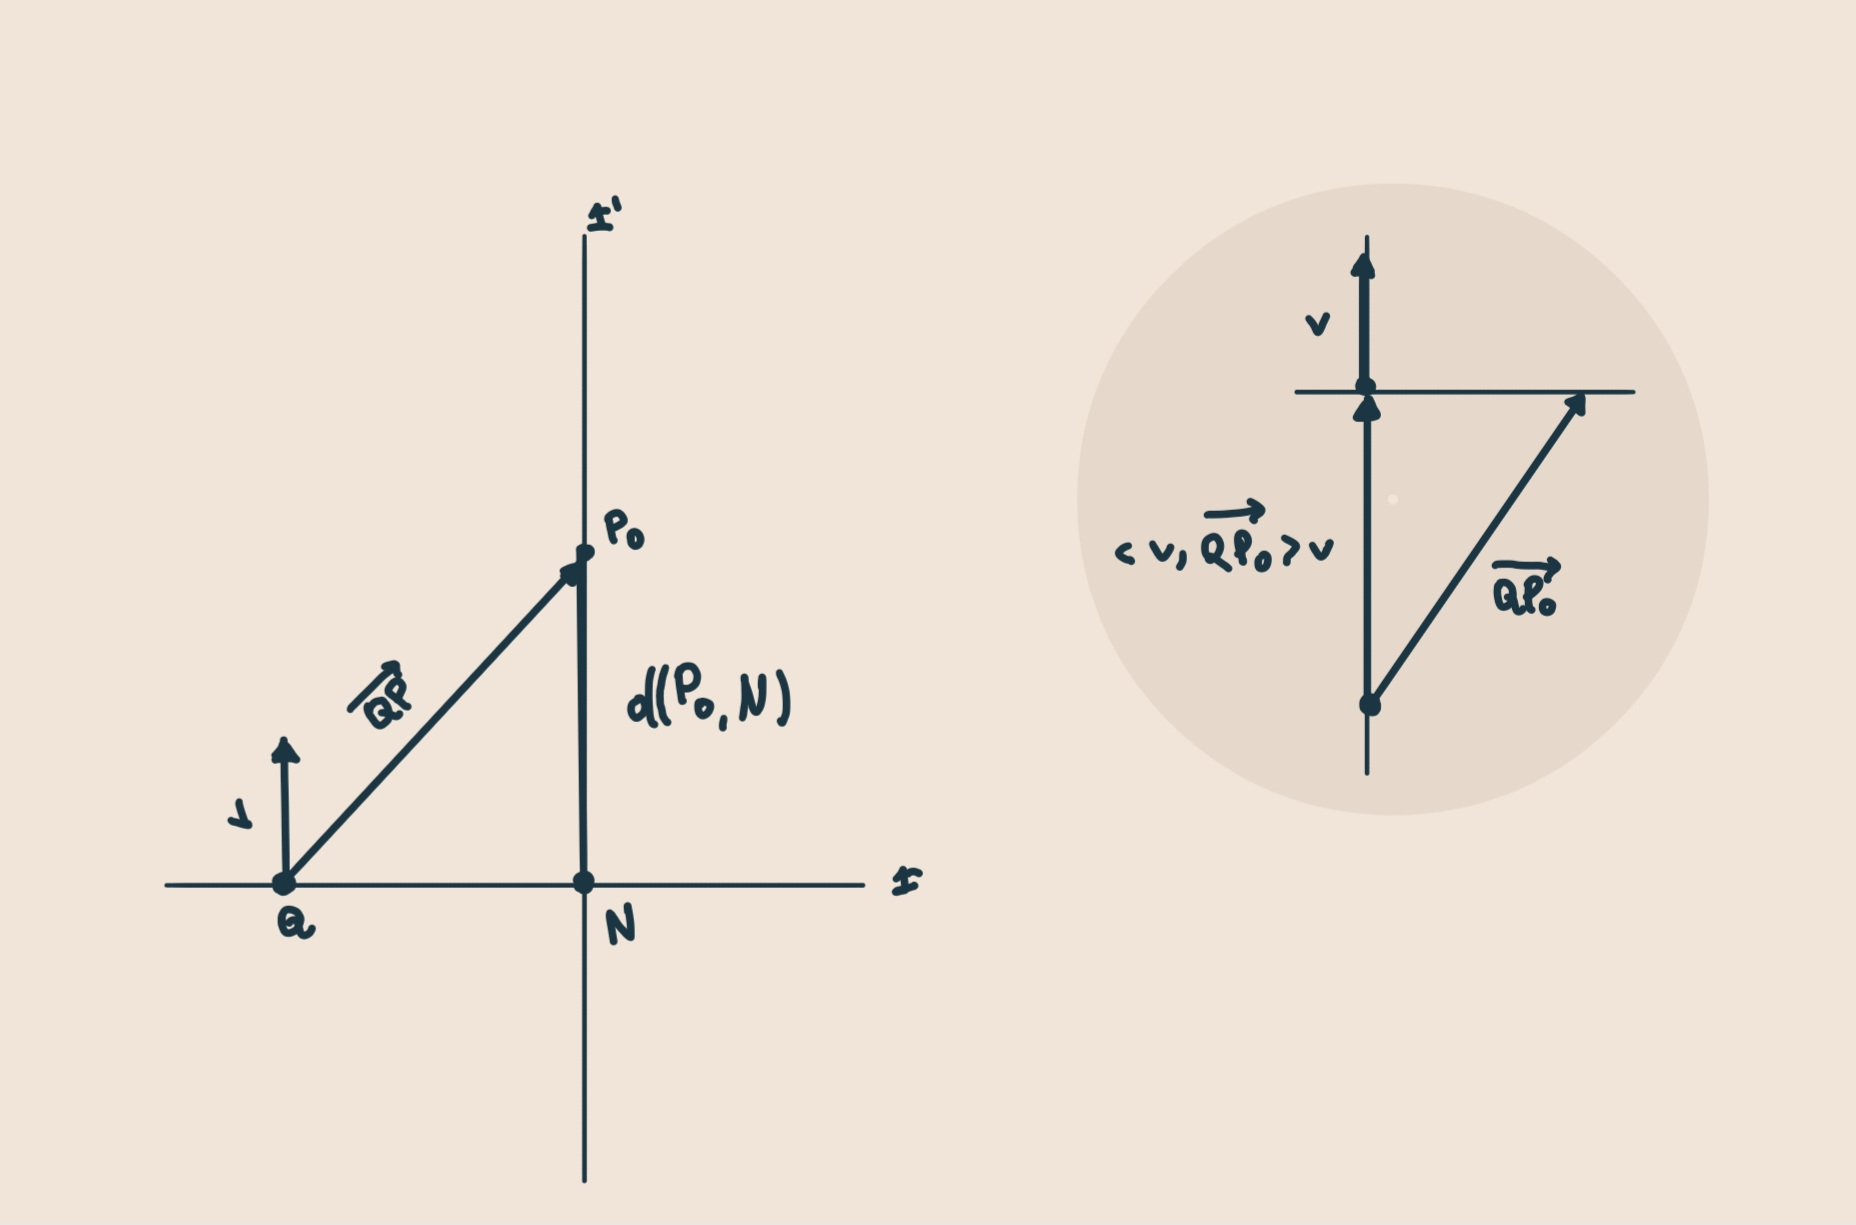
\includegraphics[scale=0.2]{proiez}    
\end{center}
Scegliamo 
\[\mathbf{v} \left( \dfrac{A}{\sqrt{A^2 + B^2}}, \dfrac{B}{\sqrt{A^2 + B^2}} \right)\]
come versore normale; 
poiché $\overrightarrow{QP_0}$ ha coordinate $(x_0 - a,\,y_0 - b)$, tenendo presente che $C = -(Aa + Bb)$, 
otteniamo
\[
d(P_0, \mathfrak{r}) = \dfrac{|A(x_0 - a) + B(y_0 - b)|}{\sqrt{A^2 + B^2}} = 
\dfrac{|Ax_0 + By_0 + C|}{\sqrt{A^2 + B^2}}.
\]
\end{proof}

\vspace{10pt}

Se $\mathfrak{r}$ ed $\mathfrak{r}'$ sono due rette parallele di $\mathbf{E}$, la loro distanza 
$d(\mathfrak{r}, \mathfrak{r}')$ è per definizione uguale a $d(P, \mathfrak{r}')$, dove $P$ è un punto 
qualunque di $\mathfrak{r}$. 
Per calcolare $d(\mathfrak{r}, \mathfrak{r}')$ è sufficiente trovare un punto $P \in \mathfrak{r}$ e 
applicare la formula della proposizione \ref{diciannovetre}.

\vspace{10pt}

Sia $\mathbf{E}$ uno spazio euclideo di dimensione $3$ con spazio vettoriale associato $\mathbf{V}$. 
Supponiamo fissato in $\mathbf{E}$ un sistema di coordinate cartesiane $O\mathbf{ijk}$.
Consideriamo un piano $\mathscr{P}$ in $\mathbf{E}$, di equazione cartesiana
\begin{equation}\label{diciannovequattro}
AX + BY + CZ + D = 0.    
\end{equation}
Un vettore $\mathbf{m}$ si dice \textbf{normale} (o \textbf{perpendicolare}, o \textbf{ortogonale}) a 
$\mathscr{P}$ se è ortogonale ad ogni vettore della giacitura di $\mathscr{P}$. 
Se inoltre $\mathbf{m}$ è un versore, esso viene detto \textbf{versore normale} a $\mathscr{P}$.

\vspace{10pt}

Poiché $\dim(\mathbf{E}) = 3$, due qualsiasi vettori normali a $\mathscr{P}$ sono tra loro paralleli; 
quindi $\mathscr{P}$ possiede esattamente due versori normali.

\vspace{10pt}

Fissiamo un punto $P_0(x_0, y_0, z_0) \in \mathscr{P}$ e consideriamo l'equazione cartesiana di $\mathscr{P}$
\begin{equation}\label{diciannovecinque}
A(X - x_0) + B(Y - y_0) + C(Z - z_0) = 0.    
\end{equation}
Ogni vettore appartenente alla giacitura di $\mathscr{P}$ è della forma 
$\overrightarrow{P_0P},\; P \in \mathscr{P}$; quindi dalla \ref{diciannovecinque} vediamo che il vettore 
$\mathbf{n}(A, B, C)$ è normale a $\mathscr{P}$. Ne deduciamo che i due vettori 
$\pm \mathbf{v} = \pm \frac{\mathbf{n}}{\|\mathbf{n}\|}$ di coordinate
\[
\pm \left( \frac{A}{\sqrt{A^2 + B^2 + C^2}}, 
\frac{B}{\sqrt{A^2 + B^2 + C^2}}, 
\frac{C}{\sqrt{A^2 + B^2 + C^2}} \right)
\]
sono i versori normali a $\mathscr{P}$.

\vspace{10pt}

La \ref{diciannovecinque} mostra inoltre che un qualsiasi piano è individuato da un suo punto 
e da un vettore ad esso perpendicolare.

\vspace{10pt}

L'angolo convesso fra due piani di $\mathbf{E}$ può essere definito utilizzando i loro vettori normali. 

\vspace{10pt}

\paragraph{Angolo convesso tra due piani}
\begin{bxthm}
\begin{defn}
Siano $\mathscr{P}$ e $\mathscr{P}'$ due piani, di equazioni cartesiane
\[AX + BY + CZ + D = 0\quad\quad A'X + B'Y + C'Z + D' = 0.\]
L'angolo convesso di $\mathscr{P}$ e $\mathscr{P}'$ è l'angolo convesso tra i vettori 
$\mathbf{n}(A,B,C)$ ed $\mathbf{n}'(A',B',C')$, cioè è l'angolo $\varphi$ definito da 
$0 \le \varphi \le \pi$ e da
\begin{equation}\label{diciannovesette}
\cos \varphi = \dfrac{\langle \mathbf{n}, \mathbf{n}' \rangle}
{\|\mathbf{n}\| \, \|\mathbf{n}'\|} = 
\dfrac{AA' + BB' + CC'}{\sqrt{A^2 + B^2 + C^2}\sqrt{A'^2 + B'^2 + C'^2}}.     
\end{equation}    
\end{defn}
\end{bxthm}

\vspace{10pt}

Si osservi che la definizione di $\varphi$ dipende dai vettori $\mathbf{n}$ ed $\mathbf{n}'$, 
e quindi dalla scelta delle equazioni dei piani. 
Moltiplicando una o l'altra per un fattore di proporzionalità negativo, 
$\varphi$ si cambia in $\pi - \varphi$.

\vspace{10pt}

Se $\varphi = \frac{\pi}{2}$ i due piani si dicono \textbf{perpendicolari} od \textbf{ortogonali}. 
Ciò avviene se e solo se
\[
AA' + BB' + CC' = 0.
\]

\vspace{10pt}

\paragraph{Angolo tra una retta e un piano}
\begin{bxthm}
\begin{defn}
Sia $\mathscr{P}$ un piano di equazione 
\[AX + BY + CZ + D = 0,\]
e sia $\mathfrak{r}$ una retta 
con vettore di direzione $\mathbf{a}(l,m,n)$. 
\textbf{L'angolo tra $\mathscr{P}$ ed $\mathfrak{r}$} è l'angolo 
la cui determinazione è
\[
\varphi = \psi - \dfrac{\pi}{2},
\]
dove $\psi$ è l'angolo convesso tra i vettori $\mathbf{n}(A,B,C)$ e $\mathbf{a}$. 
Quindi $\varphi$ è definito dalle condizioni
\[
-\dfrac{\pi}{2} \le \varphi \le \dfrac{\pi}{2}
\]
e
\[
\sin \varphi = \frac{Al + Bm + Cn}{\sqrt{A^2 + B^2 + C^2} \sqrt{l^2 + m^2 + n^2}}.
\]    
\end{defn}
\end{bxthm}

\vspace{10pt}

Se $\varphi = \pm \dfrac{\pi}{2}$, allora $\mathscr{P}$ ed $\mathfrak{r}$ si dicono 
\textbf{perpendicolari} (od \textbf{ortogonali}).

\vspace{10pt}

Si noti che ponendo $\sin \varphi = 0$ si ritrova la condizione di parallelismo 
tra $\mathscr{P}$ ed $\mathfrak{r}$
\[
Al + Bm + Cn = 0
\]
già data nella proposizione \ref{riecrui}.

\vspace{10pt}

La distanza di un punto da un piano si definisce in modo simile al caso della distanza punto-retta in un piano 
euclideo.

\vspace{10pt}

\paragraph{Distanza di un punto da un piano}
\begin{bxthm}
\begin{defn}
Siano $\mathscr{P}$ un piano di equazione 
\[AX + BY + CZ + D = 0,\]
e $P_0(x_0, y_0, z_0) \in \mathbf{E}$ un punto. 
Consideriamo la retta $\mathfrak{r}$ passante per $P_0$ e perpendicolare a $\mathscr{P}$ e denotiamo con 
$N = \mathscr{P} \cap \mathfrak{r}$ il piede della perpendicolare condotta da $P_0$ a $\mathscr{P}$. Definiamo la 
distanza di $P_0$ da $\mathscr{P}$ come
\[
d(P_0, \mathscr{P}) = d(P_0, N).
\]    
\end{defn}
\end{bxthm}

\vspace{10pt}

Si dimostra che
\[
d(P_0, \mathscr{P}) = \frac{\left| A x_0 + B y_0 + C z_0 + D \right|}{\sqrt{A^2 + B^2 + C^2}}.
\]
La dimostrazione è simile a quella della proposizione 19.3 ed è lasciata al lettore.

\vspace{10pt}

\paragraph{Distanza tra una retta e un piano paralleli}
Se $\mathfrak{r}$ e $\mathscr{P}$ sono rispettivamente una retta e un piano paralleli, la loro distanza 
$d(\mathfrak{r},\mathscr{P})$ è per definizione $d(P, \mathscr{P})$, dove $P$ è un qualsiasi punto di 
$\mathfrak{r}$. Per calcolare $d(\mathfrak{r},\mathscr{P})$ è sufficiente trovare le coordinate di un punto
$P \in \mathfrak{r}$ e applicare la formula che dà $d(P, \mathscr{P})$.

\vspace{10pt}

\paragraph{Distanza di un punto da una retta}
\begin{bxthm}
\begin{defn}
Sia $\mathfrak{r}$ una retta e sia $P_0 \in \mathbf{E}$. Consideriamo il piano $\mathscr{P}$ passante per $P_0$ e 
perpendicolare a $\mathfrak{r}$ e sia $N = \mathfrak{r} \cap \mathscr{P}$. La distanza di $P_0$ da $\mathfrak{r}$ è definita come
\[
d(P_0, \mathfrak{r}) = d(P_0, N).
\]    
\end{defn}
\end{bxthm}

\vspace{10pt}

Se $\mathfrak{r}$ passa per il punto $Q(a, b, c)$ e ha vettore di direzione $\mathbf{a}(l, m, n)$, e 
$P_0(x_0, y_0, z_0) \in \mathbf{E}$, allora si ha la seguente formula:
\[
d(P_0, \mathfrak{r}) =
\dfrac{\sqrt{\begin{vmatrix}y_0-b&z_0-c\\m&n\end{vmatrix}^2+\begin{vmatrix}x_0-a&z_0-c\\l&n\end{vmatrix}^2+\begin{vmatrix}x_0-a&y_0-b\\l&m\end{vmatrix}^2}}{\sqrt{l^2 + m^2 + n^2}}
\]
Infatti
\[
\overrightarrow{QP_0} = \overrightarrow{QN} + \overrightarrow{NP_0},
\]
e $\overrightarrow{QN}$ è parallelo ad $\mathbf{a}$, mentre $\overrightarrow{NP_0}$ è perpendicolare ad $\mathbf{a}$.

Dalla proposizione \ref{diciottoquattro} si deduce che
\[
d(P_0, \mathfrak{r}) = \|\overrightarrow{NP_0}\| = \dfrac{\|\mathbf{a} \wedge \overrightarrow{QP_0}\|}{\|\mathbf{a}\|}.
\]

Esplicitando l'uguaglianza si ottiene l'asserto.

\vspace{10pt}

\paragraph{Distanza tra due rette}
Date due rette \(\mathfrak{r}\) ed \(\mathfrak{r}'\) non parallele in \(\mathbf{E}\), definiamo la loro distanza, 
che denoteremo con \(d(\mathfrak{r}, \mathfrak{r}')\), nel modo seguente.
Supponiamo che \(\mathfrak{r}\) passi per il punto \(Q(a, b, c)\) e abbia \(\mathbf{a}(l, m, n)\) come vettore 
di direzione, e che \(\mathfrak{r}'\) passi per \(Q'(a', b', c')\) e abbia vettore di direzione 
\(\mathbf{a}'(l', m', n')\).

Osserviamo che esiste una e una sola coppia di punti, \(N \in \mathfrak{r}\) ed \(N' \in \mathfrak{r}'\), 
tali che la retta che li contiene sia perpendicolare sia a \(\mathfrak{r}\) che a \(\mathfrak{r}'\). 
Infatti le due condizioni di perpendicolarità sono
\begin{equation}\label{diciannoveotto}
\langle \overrightarrow{N N'}, \mathbf{a} \rangle = 0
\quad\quad
\langle \overrightarrow{N N'}, \mathbf{a}' \rangle = 0    
\end{equation}
Scrivendo
\[
\overrightarrow{O N} = \overrightarrow{O Q} + t \mathbf{a}
\quad
\overrightarrow{O N'} = \overrightarrow{O Q'} + t' \mathbf{a}',
\]
si ottiene
\[
\overrightarrow{N N'} = \overrightarrow{Q Q'} + t' \mathbf{a}' - t \mathbf{a},
\]
e quindi le \ref{diciannoveotto} diventano
\[
\langle \overrightarrow{Q Q'} + t' \mathbf{a}' - t \mathbf{a}, \mathbf{a} \rangle = 0
\quad
\langle \overrightarrow{Q Q'} + t' \mathbf{a}' - t \mathbf{a}, \mathbf{a}' \rangle = 0,
\]
cioè
\begin{equation}\label{diciannovenove}
\langle \overrightarrow{Q Q'}, \mathbf{a} \rangle
+ t' \langle \mathbf{a}', \mathbf{a} \rangle
- t \langle \mathbf{a}, \mathbf{a} \rangle = 0\quad\quad
\langle \overrightarrow{Q Q'}, \mathbf{a}' \rangle
+ t' \langle \mathbf{a}', \mathbf{a}' \rangle
- t \langle \mathbf{a}, \mathbf{a}' \rangle = 0.
\end{equation}
Poiché \(\mathbf{a}\) ed \(\mathbf{a}'\) sono linearmente indipendenti, per il teorema \ref{diciottodue}(6) si ha
\[
\begin{vmatrix}
\langle \mathbf{a}', \mathbf{a} \rangle & \langle \mathbf{a}, \mathbf{a} \rangle\\
\langle \mathbf{a}', \mathbf{a}' \rangle & \langle \mathbf{a}, \mathbf{a}' \rangle
\end{vmatrix}
= \|\mathbf{a} \wedge \mathbf{a}'\|^2 \neq 0.
\]
Quindi il sistema \eqref{diciannovenove} ammette una e una sola soluzione \((t, t')\), e ciò significa appunto che 
esiste un'unica coppia \((N, N')\) che soddisfa alla condizione voluta.

\vspace{10pt}

La retta \(\mathfrak{s}\) passante per \(N\) e per \(N'\) si chiama \textbf{perpendicolare comune} a 
\(\mathfrak{r}\) e a \(\mathfrak{r}'\).

\vspace{10pt}

Ciò posto, definiamo la \textbf{distanza di \(\mathfrak{r}\) da \(\mathfrak{r}'\)} come
\[
d(\mathfrak{r}, \mathfrak{r}') = d(N, N').
\]
Si ha la seguente formula che permette di calcolare agevolmente la distanza di due rette assegnate:
\begin{equation}\label{diciannovedieci}
d(\mathfrak{r}, \mathfrak{r}') = 
\dfrac{
\begin{vmatrix}
a - a' & b - b' & c - c'\\
l & m & n\\
l' & m' & n'
\end{vmatrix}
}
{
\sqrt{
\begin{vmatrix}
m & n\\
m' & n'
\end{vmatrix}^2
+
\begin{vmatrix}
l & n\\
l' & n'
\end{vmatrix}^2
+
\begin{vmatrix}
l & m\\
l' & m'
\end{vmatrix}^2
}
}
\end{equation}
La \eqref{diciannovedieci} si dimostra nel modo seguente.
Sia \(\mathbf{b}\) un versore della perpendicolare comune a \(\mathfrak{r}\) e a \(\mathfrak{r}'\). Si ha
\[
\langle \mathbf{b}, \overrightarrow{Q Q'} \rangle
= \langle \mathbf{b}, \overrightarrow{Q N} \rangle 
+ \langle \mathbf{b}, \overrightarrow{N Q'} \rangle 
= \langle \mathbf{b}, \overrightarrow{N Q'} \rangle
\]
e quindi
\[
d(\mathfrak{r}, \mathfrak{r}')
= | \langle \mathbf{b}, \overrightarrow{N Q'} \rangle |
= | \langle \mathbf{b}, \overrightarrow{Q Q'} \rangle |.
\]
D'altra parte, poiché \(\mathbf{b}\) è ortogonale sia ad \(\mathbf{a}\) che ad \(\mathbf{a}'\), si ha
\[
\mathbf{b} = \pm \frac{\mathbf{a} \wedge \mathbf{a}'}{\|\mathbf{a} \wedge \mathbf{a}'\|}.
\]
Quindi
\[
d(\mathfrak{r}, \mathfrak{r}')
= \frac{|\langle \mathbf{a} \wedge \mathbf{a}', \overrightarrow{Q Q'} \rangle|}{\|\mathbf{a} \wedge \mathbf{a}'\|}.
\]
Esplicitando quest'uguaglianza si ottiene la formula cercata.

\vspace{10pt}

Per trovare equazioni cartesiane della retta $\mathcal{s}$ perpendicolare comune a $\mathfrak{r}$ e a 
$\mathfrak{r}'$ si procede nel modo seguente.
Conosciamo $\mathbf{a}\wedge\mathbf{a}'$, vettore di direzione $\mathfrak{s}$, le cui coordinate 
denotiamo con $(\beta_1, \beta_2, \beta_3)$. Denotando con $P(X, Y, Z)$ un punto di coordinate indeterminate, 
e imponendo le condizioni di complanarità di $\mathfrak{r}$ e di $\mathfrak{r}'$ con la retta passante per 
$P$ e avente vettore di direzione $\mathbf{a}\wedge\mathbf{a}'$, otteniamo le due seguenti equazioni:
\[
    \begin{vmatrix}
    X - a & Y - b & Z - c \\\\
    \beta_1 & \beta_2 & \beta_3 \\\\
    l & m & n
    \end{vmatrix} = 0\quad\quad
    \begin{vmatrix}
    X - a' & Y - b' & Z - c' \\\\
    \beta_1 & \beta_2 & \beta_3 \\\\
    l' & m' & n'
    \end{vmatrix} = 0.
\]
Poiché queste equazioni rappresentano due piani distinti e sono soddisfatte dai punti di $\mathfrak{s}$, 
esse sono equazioni cartesiane di $\mathfrak{s}$.

\vspace{20pt}

Supponiamo fissato in uno spazio euclideo $\mathbf{E}$ un riferimento cartesiano 
$O\mathbf{e}_1 \ldots \mathbf{e}_n$ ed un punto $C(c_1, \ldots, c_n)$. Sia $r > 0$.
\begin{itemize}
    \item La \textbf{sfera di centro $C$ e raggio $r$} è l'insieme
        \[\mathbf{S}(C, r)=\{P(x_1, \ldots, x_n)\in\mathbf{E}\,:\;d(C, P) = r\},\]
        cioè tali che
        \begin{equation}\label{diciannoveundici}
        \sum_{i=1}^{n}(x_i - c_i)^2 = r^2.
        \end{equation}
    \item Il \textbf{disco di centro $C$ e raggio $r$} è l'insieme
        \[\mathbf{D}(C, r)=\{P(x_1, \ldots, x_n)\in\mathbf{E}\,:\;d(C, P) \leq r\},\]
        cioè tali che
        \begin{equation}
        \sum_{i=1}^{n}(x_i - c_i)^2 \leq r^2.
        \end{equation}
\end{itemize}

\vspace{10pt}

Nel caso in cui $\mathbf{E}$ sia un piano, $\mathbf{S}(C, r)$ e $\mathbf{D}(C, r)$ sono la 
\textbf{circonferenza} e il \textbf{cerchio} rispettivamente, di centro $C$ e raggio $r$.
Se $\dim(\mathbf{E}) = 1$, $\mathbf{D}(C, r)$ è il segmento di lunghezza $2r$ e di centro $C$, ed 
$\mathbf{S}(C, r)$ è l'insieme costituito dai suoi estremi.

\vspace{10pt}

Quando $\mathbf{E} = \mathbf{E}^n$, si usano i simboli $\mathbf{S}^{n-1}$ e $\mathbf{D}^n$ per denotare 
$\mathbf{S}(\mathbf{0}, 1)$ e $\mathbf{D}(\mathbf{0}, 1)$ rispettivamente.

\vspace{10pt}

Dalla \ref{diciannoveundici} deduciamo che $\mathbf{S}(C, r)$ è l'insieme dei punti di $\mathbf{E}$ le cui 
coordinate sono soluzioni dell'equazione
\begin{equation}\label{diciannovedodici}
\sum_{i=1}^{n}(X_i - c_i)^2 = r^2 
\end{equation}
nelle indeterminate $X_1, X_2, \ldots, X_n$. La \ref{diciannovedodici} è detta \textbf{equazione cartesiana della sfera $\mathbf{S}(C, r)$}. 
Portando $r^2$ a primo membro e svolgendo i calcoli troviamo che la \ref{diciannovedodici} è equivalente 
all'equazione
\begin{equation}\label{diciannovetredici}
\sum_{i=1}^{n}X_i(X_i+d_i) + d = 0\quad\quad\quad d_i = -2c_i,\quad d = \sum_{i=1}^{n}c_i^2 - r^2.
\end{equation}
A causa della loro definizione 
e del fatto che $r^2 > 0$, i coefficienti $d_1, \ldots, d_n, d$ della \ref{diciannovetredici} soddisfano la condizione
\begin{equation}\label{diciannovequattordici}
\sum_{i=1}^{n}\dfrac{d_i^2}{4} - d > 0.
\end{equation}
Viceversa, un'equazione della forma \ref{diciannovetredici} i cui coefficienti soddisfano la condizione 
\ref{diciannovequattordici} è equazione cartesiana di una sfera $\mathbf{S}$, il cui centro 
$C(c_1, \ldots, c_n)$ e raggio $\rho$ sono
\[c_i = -\frac{d_i}{2}, \quad r = \sqrt{\sum_{i=1}^{n}\dfrac{d_i^2}{4} - d}.\]
Nel caso particolare $n = 2$, la \ref{diciannovetredici} è l'equazione di una circonferenza e ha la forma, 
nelle indeterminate $X$, $Y$,
\begin{equation}\label{diciannovequindici}
X^2 + Y^2 + d_1 X + d_2 Y + d = 0 \quad\quad\quad\dfrac{d_1^2}{4} + \dfrac{d_2^2}{4} - d > 0.
\end{equation}
Il centro della circonferenza è 
\[C\left(-\frac{d'}{2}, -\frac{d_2}{2}\right),\]
mentre il raggio è
\[r = \sqrt{\dfrac{d_1^2}{4} + \frac{d_2^2}{4} - d}.\]

\vspace{10pt}

Sia $\mathbf{E}$ un piano euclideo in cui sia assegnata un'orientazione (un piano euclideo orientato) e siano 
$\mathfrak{s}$ ed $\mathfrak{s}'$ due semirette aventi origine nello stesso punto $O$. Detti 
$\mathbf{a}$ e $\mathbf{a}'$ vettori di direzione di $\mathfrak{s}$ ed $\mathfrak{s}'$ rispettivamente, 
l'angolo $\widehat{\mathbf{a}\mathbf{a}'}$ si dice \textbf{angolo orientato tra $\mathfrak{s}$ ed $\mathfrak{s}'$} e si denota 
con $\widehat{\mathfrak{s}\mathfrak{s}'}$.

\vspace{10pt}

In un piano euclideo orientato $\mathbf{E}$ fissiamo una semiretta $\mathfrak{s}$ di origine $O$. 
Per ogni punto $P \neq O$ lo associamo al piano $E$ consideriamo la semiretta $\mathfrak{s}_P$ di origine 
$O$ e vettore di direzione $\overrightarrow{OP}$. Lo scalare positivo $\rho = \|\overrightarrow{OP}\|$, 
e l'angolo $\theta = \widehat{\mathfrak{s}\mathfrak{s}_P}$ si dicono \textbf{coordinate polari} di $P$, e 
rispettivamente il \textbf{modulo} e l'\textbf{anomalia} di $P$ rispetto alla semiretta $\mathfrak{s}$. 
Diremo che $\mathfrak{s}$ definisce in $\mathbf{text}E$ un \textbf{sistema di coordinate polari}.
Le coordinate polari $(\rho, \theta)$ di un punto $P \neq O$ lo individuano univocamente. Infatti $\theta$ 
individua una semiretta $\mathfrak{s}_\theta$ di origine $O$, e $P$ è il punto di intersezione di 
$\mathfrak{s}_\theta$ con la circonferenza di centro $O$ e raggio $\rho$.
Quindi per ogni coppia di numeri reali $(\rho, \theta)$, con $\rho > 0$, esiste un unico punto $P$ le cui 
coordinate polari sono $\rho$ e l'angolo definito da $\theta$. Si conviene di estendere le coordinate polari 
anche al punto $O$ assegnandogli modulo $\rho = 0$ ed anomalia indeterminata.
Consideriamo il riferimento cartesiano $O\mathbf{ij}$ appartenente all'orientazione assegnata in 
$\mathbf{E}$, avente origine in $O$ e tale che $\mathbf{i}$ sia il versore di direzione di $\mathfrak{s}$. 
($O\mathbf{ij}$ è univocamente individuato da queste condizioni). Sia $P \neq O$ un punto avente coordinate 
polari $(\rho, \theta)$ e coordinate cartesiane $(x, y)$. Allora si ha
\begin{equation}\label{diciannovesedici}
x = \rho \cos \theta \quad\quad y = \rho \sin \theta.    
\end{equation}
Viceversa:
\begin{equation}\label{diciannovediciassette}
\rho = \sqrt{x^2 + y^2}\quad\quad\theta = \varepsilon(y) \arccos \left( \frac{x}{\sqrt{x^2 + y^2}} \right),     
\end{equation}
in cui si è denotato con $\varepsilon(y) = \pm 1$ a seconda che $y \geq 0$ oppure $y < 0$ (con questa formula si 
individua una determinazione dell'angolo $\theta$ compresa tra $-\pi$ e $\pi$).
Le \ref{diciannovesedici} e \ref{diciannovediciassette} sono le 
\textbf{formule di passaggio da coordinate polari a coordinate cartesiane e viceversa}. La validità delle 
suddette formule è lasciata al lettore.

\vspace{10pt}

Sia $\mathbf{E}$ uno spazio euclideo di dimensione $n$, $O \mathbf{e}_1 \ldots \mathbf{e}_n$ un riferimento cartesiano, e 
siano 
\[A_i(a_1^i, \ldots, a_n^i)\in\mathbf{E},\quad\quad i\in\{0,1,\ldots,n\}, \]
punti indipendenti. Il \textbf{volume dell'$n$-parallelepipedo} rispettivamente determinato da 
$A_0, A_1, \ldots, A_n$ è definito come $|\det(M)|$, dove
\[M = \begin{pmatrix}
a_1^1 - a_1^0 & a_2^1 - a_2^0 & \cdots & a_1^n - a_n^0 \\\\
a_1^2 - a_1^0 & a_2^2 - a_2^0 & \cdots & a_2^n - a_n^0 \\\\
\vdots & \vdots & \ddots & \vdots \\\\
a_1^n - a_1^0 & a_2^n - a_2^0 & \cdots & a_n^n - a_n^0
\end{pmatrix}.\]
In particolare, per $n = 1, 2, 3$ parleremo di \textbf{lunghezza}, \textbf{area}, \textbf{volume} di un segmento, 
di un parallelogramma, di un parallelepipedo rispettivamente. La lunghezza di un segmento $A(a)B(b)$ di una 
retta euclidea è $|b - a|$, quindi coincide con $d(A, B)$.
L'area del parallelogramma individuato da $A(a_1, a_2)$, $B(b_1, b_2)$, $C(c_1, c_2)$ in un piano euclideo è
\[\begin{vmatrix}
b_1 - a_1 & b_2 - a_2 \\
c_1 - a_1 & c_2 - a_2
\end{vmatrix}.\]
Il volume del parallelepipedo individuato da 
$A(a_1, a_2, a_3)$, $B(b_1, b_2, b_3)$, $C(c_1, c_2, c_3)$, $D(d_1, d_2, d_3)$ in uno spazio euclideo di 
dimensione $3$ è
\[\begin{vmatrix}
b_1 - a_1 & b_2 - a_2 & b_3 - a_3 \\
c_1 - a_1 & c_2 - a_2 & c_3 - a_3 \\
d_1 - a_1 & d_2 - a_2 & d_3 - a_3
\end{vmatrix}.\]
Osserviamo che la definizione di volume di un $n$-parallelepipedo non dipende dalla scelta del riferimento 
cartesiano $O\mathbf{e}_1 \ldots \mathbf{e}_n$. Infatti le righe della matrice $M$ sono le coordinate dei 
vettori $\overrightarrow{A_0A_1},\overrightarrow{A_0A_2},\ldots,\overrightarrow{A_0A_n}$ rispetto 
alla base $\{\mathbf{e}_1, \ldots, \mathbf{e}_n\}$; se $O\mathbf{f}_1 \ldots \mathbf{f}_n$ è un altro 
riferimento cartesiano, le coordinate di 
$\overrightarrow{A_0A_1},\overrightarrow{A_0A_2},\ldots,\overrightarrow{A_0A_n}$ 
rispetto alla base $\{\mathbf{f}_1, \ldots, \mathbf{f}_n\}$ si ottengono dalle 
precedenti moltiplicando per una matrice ortogonale. Quindi la matrice $N$ analoga di $M$ nel riferimento 
$O\mathbf{f}_1 \ldots \mathbf{f}_n$ si ottiene da $M$ moltiplicandola a destra per una matrice ortogonale, 
che ha determinante uguale a $\pm 1$; dunque
\[|\det(M)| = |\det(N)|.\]

\vspace{10pt}

\paragraph{Sottoinsieme limitato}
\begin{bxthm}
\begin{defn}
Sia $\mathbf{E}$ uno spazio euclideo. Un sottoinsieme $\mathbf{S} \subset \mathbf{E}$ si dice \textbf{limitato} se è 
contenuto in un disco, cioè
\[\exists\,C \in \mathbf{E}\,\land\,r>0\,:\;\mathbf{S} \subset D(C, r).\]
\end{defn}
\end{bxthm}

\vspace{10pt}

Un \textbf{poliedro convesso} è un sottoinsieme limitato di $\mathbf{E}$ che non è contenuto in un sottospazio 
affine proprio di $\mathbf{E}$ e che è l'intersezione di un numero finito di semispazi. Un poliedro convesso 
è un insieme convesso perché lo è ogni semispazio. La dimensione di $\mathbf{E}$ è detta 
\textbf{dimensione del poliedro}. Se $\dim(\mathbf{E}) = 1$ si ottiene un segmento. Se $\dim(\mathbf{E}) = 2$, 3 
un poliedro convesso si dice \textbf{poligono convesso} e \textbf{solido convesso} rispettivamente.

\vspace{10pt}

Lasciamo al lettore di introdurre in modo appropriato tutte le nozioni elementari relative ai poligoni convessi, 
come quelle di \emph{vertice}, \emph{lato} ed \emph{angolo}, di $n$-\emph{agono regolare}, di \emph{lati adiacenti} 
o \emph{consecutivi} ecc. in analogia con quanto viene fatto in geometria euclidea elementare.

\vspace{10pt}

Supponiamo $\dim(\mathbf{E}) = 3$ e sia $\Pi \subset \mathbf{E}$ un solido convesso. Se $\mathscr{I}$ è un 
piano di $\mathbf{E}$ tale che $\Pi$ sia contenuto in uno dei due semispazi definiti da $\mathscr{I}$, allora 
abbiamo le seguenti possibilità:
\begin{itemize}
\item $\mathscr{I}\cap\Pi = \emptyset$;
\item $\mathscr{I}\cap\Pi$ è un punto, che si dice \textbf{vertice} di $\Pi$;
\item $\mathscr{I}\cap\Pi$ è un segmento, che si dice \textbf{spigolo} (o \textbf{lato}) di $\Pi$;
\item $\mathscr{I}\cap\Pi$ è un poligono, che si dice \textbf{faccia} di $\Pi$.
\end{itemize}

\vspace{10pt}

Dal fatto che $\Pi$ è intersezione di un numero finito di semispazi segue che esso possiede un numero 
finito $v$ di vertici, $s$ di spigoli, ed $f$ di facce. 
È facile vedere che ogni spigolo è lato di due facce e ogni vertice è vertice di almeno tre facce e di altrettanti spigoli.

\vspace{10pt}

Per ogni solido convesso $\Pi$ sussiste la seguente relazione tra $v$, $s$ ed $f$:
\begin{equation}\label{diciannovediciotto}
v - s + f = 2. 
\end{equation}

\vspace{10pt}

Daremo una dimostrazione della \ref{diciannovediciotto} che è simile a quella originale di Eulero. Per semplificare l'argomentazione supporremo 
che sia possibile costruire il solido $\Pi$ partendo da una faccia e aggiungendone poi via via altre, in 
modo che ad ogni nuova faccia che si aggiunge abbia solo lati \textbf{adiacenti} in comune con quelle precedentemente 
iscritte.

\vspace{10pt}

Si osservi che necessariamente $f \geq 3$. Ad ogni stadio del procedimento denotiamo con $\Phi$ il numero 
$v - s + f - 1$. Per una sola faccia si ha $v = 0$. Procediamo per induzione sul numero di facce iscritte, 
dimostrando che finché il poliedro non è stato completato, si ha $\Phi = 0$. Supponiamo che ciò sia vero un 
dato stadio della costruzione in cui restano da iscrivere almeno due facce ancora. Aggiungendo una nuova faccia 
$F$ avente $p$ lati, di cui $q$ consecutivi siano in comune con le precedenti; pertanto $q + 1$ vertici di 
$F$ appartengono alle precedenti facce. Abbiamo quindi aggiunto 1 nuova faccia, $p - q$ nuovi vertici, 
$p - q$ nuovi spigoli. Denotando con $\Phi'$ la quantità corrispondente di $\Phi$ relativa alla nuova configurazione, 
si ha
\begin{align}
\Phi' &= \Phi + (p - q) - (p - q) + 1 = \Phi + 1 = 0 + 1 = 1 = \Phi,
\end{align}
come asserito. Osserviamo che quando si aggiunge l'ultima faccia non si modifica né il numero dei vertici 
né quello degli spigoli, mentre il numero delle facce aumenta di 1. Quindi per $\Pi$ si ha $\Phi = 1$, 
cioè la (19.18).

Gli studi sulla estensione 3-dimensionale dei poligoni regolari detti ``solidi regolari''. Un 
\textit{solido regolare} è un solido convesso avente facce poligonali tutti uguali tra loro. È un fatto 
notevole che, diversamente da quello che avviene per i poligoni regolari, esistono solo un numero finito, 
precisamente 5, di classi di similitudine di solidi regolari (per la definizione di similitudine cfr. 
20.10(2)): il \textit{tetraedro}, l'\textit{ottaedro}, il \textit{cubo}, il \textit{dodecaedro}, 
l'\textit{icosaedro} (fig. 19.4).

Questi solidi erano noti fin dall'antichità. Poiché la scuola platonica se ne interessò, in particolare 
Platone ne parla nel \textit{Timeo}, essi vengono anche chiamati \textit{solidi platonici}. Teeteto li 
studiò sistematicamente attorno al 380 a.C. e di essi tratta il XIII libro degli \textit{Elementi} di 
Euclide. (Per maggiori dettagli rimandiamo il lettore a [7]).

\vspace{50pt}
\section{Diagonalizzazione di operatori simmetrici}
\vspace{20pt}

Nelle pagine precedenti abbiamo introdotto due diverse relazioni di equivalenza tra matrici quadrate: 
la similitudine e la congruenza. Due matrici $A,B \in M_n(\mathbb{K})$, $n \geq 1$, sono dette simili
(rispettivamente congruenti) se 
\[\exists\,M \in \mathrm{GL}_n(\mathbb{K})\,:\;B = M^{-1}AM \;(B = {}^tMAM).\]

\vspace{10pt}

La similitudine è stata introdotta allo scopo di studiare le matrici che rappresentano un operatore su di 
uno spazio vettoriale rispetto a due diverse basi; la congruenza è stata invece definita per descrivere le 
matrici di una forma bilineare rispetto a basi diverse.

\vspace{10pt}

In corrispondenza alle due nozioni si hanno due diversi problemi di diagonalizzazione, che possono così 
enunciarsi: data $A \in M_n(\mathbb{K})$, trovare una matrice diagonale $B \in M_n(\mathbb{K})$ simile 
(oppure congruente) ad $A$.

\vspace{10pt}

Il secondo problema, quello dell'esistenza di matrici diagonali in una data classe di congruenza, 
equivalente al problema della diagonalizzazione delle forme bilineari, è risolubile se ci si limita a 
considerare forme bilineari simmetriche, e cioè matrici $A$ simmetriche, per le quali si afferma il 
teorema \ref{sediciunoo}.

\vspace{10pt}

Come sappiamo, facili esempi mostrano che il primo dei due problemi non ammette soluzione in generale, 
cioè non tutte le classi di similitudine contengono una matrice diagonale.

\vspace{10pt}

In questo paragrafo considereremo un'altra questione, più particolare ma molto importante in geometria 
euclidea, vale a dire il problema di diagonalizzare matrici simmetriche reali per mezzo di matrici ortogonali.

\vspace{10pt}

Se $A \in M_n(\mathbb{R})$ e $M \in \mathrm{O}$, si ha
\begin{equation}\label{ventidueuno}
M^{-1}AM = {}^tMAM 
\end{equation}
e quindi la matrice \ref{ventidueuno} è simultaneamente simile e congruente ad $A$. Parlando di diagonalizzazione 
di una matrice per mezzo di matrici ortogonali, non è dunque necessario specificare se ci si riferisce 
alla similitudine o alla congruenza perché le due nozioni sono equivalenti. Il limitarsi a considerare le 
matrici $M \in \mathrm{O}(n)$ è equivalente a considerare, in uno spazio vettoriale euclideo di dimensione finita 
$\mathbf{V}$, solo basi ortonormali; quindi la diagonalizzabilità di una matrice simmetrica $A$ per mezzo di matrici 
ortogonali significa che sia la forma quadratica definita da $A$ che l'operatore di matrice $A$ rispetto a 
una base ortonormale di $\mathbf{V}$ sono diagonalizzabili in una base ortonormale.

\vspace{10pt}

Una semplice, ma fondamentale, proprietà delle matrici simmetriche reali è descritta dal seguente lemma.

\vspace{10pt}

\begin{bxthm}
\begin{lem}
Il polinomio caratteristico di una matrice simmetrica $A \in M_n(\mathbb{R})$ possiede solo radici reali.
\end{lem}    
\end{bxthm}
\begin{proof}
Possiamo considerare $A$ come una matrice di numeri complessi e quindi come un operatore 
\[T_A : \mathbb{C}^n \to \mathbb{C}^n. \]
Sia $\lambda \in \mathbb{C}$ una radice del polinomio caratteristico 
di $A$, e sia $\mathbf{x} \in \mathbb{C}^n$ un corrispondente autovettore. Si ha
\begin{equation}\label{ventiduedue}
A\mathbf{x} = \lambda \mathbf{x}.
\end{equation}
Prendendo i complessi coniugati di primo e secondo membro, si ha anche
\begin{equation}\label{ventiduetre}
A\overline{\mathbf{x}} = \overline{\lambda}\overline{\mathbf{x}}.
\end{equation}
Consideriamo lo scalare ${}^t\overline{\mathbf{x}}A\mathbf{x}$, e scriviamolo in due modi diversi 
utilizzando la \ref{ventiduedue} e la \ref{ventiduetre}:
\begin{equation}\label{ventiduequattro}
{}^t\overline{\mathbf{x}}A\mathbf{x} = {}^t\overline{\mathbf{x}}(A\mathbf{x}) = {}^t\overline{\mathbf{x}}\lambda\mathbf{x} = \lambda{}^t\overline{\mathbf{x}}\mathbf{x}    
\end{equation}
\begin{equation}\label{ventiduecinque}
{}^t\overline{\mathbf{x}}A\mathbf{x} = ({}^t\overline{\mathbf{x}}A)\mathbf{x} = {}^t(A\overline{\mathbf{x}})\mathbf{x} = {}^t(\overline{\lambda}\overline{\mathbf{x}})\mathbf{x}=\overline{\lambda}{}^t\overline{\mathbf{x}}\mathbf{x}.
\end{equation}
Osservando che
\[{}^t\overline{\mathbf{x}}\mathbf{x} = \sum_{i=1}^{n}\overline{x_i}x_i\]
è un numero reale positivo, perché $\mathbf{x} \neq \mathbf{0}$, dalle \ref{ventiduequattro} e \ref{ventiduecinque} deduciamo che 
$\lambda = \overline{\lambda}$, cioè che $\lambda$ è reale.
\end{proof}

\vspace{10pt}

\paragraph{Teorema Spettrale}
\begin{bxthm}
\begin{thm}
Siano $\mathbf{V}$ uno spazio vettoriale euclideo di dimensione finita e $T: \mathbf{V} \to \mathbf{V}$ un 
operatore simmetrico. Esiste una base ortonormale di $\mathbf{V}$ rispetto alla quale la matrice che rappresenta $T$ è diagonale.
\end{thm}    
\end{bxthm}
\begin{proof}
Procediamo per induzione su $n = \dim(\mathbf{V})$. Se $n = 1$ non c'è niente da dimostrare; supponiamo quindi 
$n \geq 2$ e che il teorema sia vero per spazi di dimensione $n-1$. Poiché l'operatore $T$ è simmetrico, il polinomio caratteristico di $T$
possiede radici reali, per il lemma \ref{ventidueuno}. Quindi $T$ possiede un autovalore $\lambda$; sia 
$\mathbf{e}_1$ un corrispondente autovettore, che possiamo supporre di norma 1, e sia 
$\mathbf{U} = \{\mathbf{e}_1\}^{\perp}$ il complemento ortogonale di $\mathbf{e}_1$. Per ogni 
$\mathbf{u} \in \mathbf{U}$ si ha
\[\langle T(\mathbf{u}), \mathbf{e}_1 \rangle = \langle \mathbf{u}, T(\mathbf{e}_1) \rangle = \langle \mathbf{u}, \lambda \mathbf{e}_1 \rangle = \lambda \langle \mathbf{u}, \mathbf{e}_1 \rangle = \lambda \cdot 0 = 0,\]
e quindi $T(\mathbf{u}) \in \mathbf{U}$, cioè $T$ induce un operatore $T_\mathbf{U} : \mathbf{U} \to \mathbf{U}$. Poiché $T_\mathbf{U}(\mathbf{u}) = T(\mathbf{u})$ per ogni 
$\mathbf{u} \in \mathbf{U}$, l'operatore $T_\mathbf{U}$ è simmetrico. Per l'ipotesi induttiva, $\mathbf{U}$ 
possiede una base ortonormale $\{\mathbf{e}_2, \ldots, \mathbf{e}_n\}$ che diagonalizza $T_\mathbf{U}$. 
Allora $\{\mathbf{e}_1, \mathbf{e}_2, \ldots, \mathbf{e}_n\}$ è una base ortonormale di $\mathbf{V}$ che diagonalizza $T$.
\end{proof}

\end{document}
